%!TEX TS-program = xelatex
%!TEX encoding = UTF-8 Unicode

% nobib: Don't load natbib with the tufte-book class, since we use biblatex instead.
\documentclass[justified,nobib]{tufte-book}
\morefloats
\usepackage{lgrind}    % syntax highlighting for source code (unused?)
\usepackage{graphicx}  % adds options to \includegraphics
\usepackage{booktabs}  % prettier tables
\usepackage{multirow}  % allow cells to span rows
\usepackage{moreverb}  % better verbatim environment (unused?)
\usepackage{alltt}     % alternative verbatim environment (unused?)
\usepackage{url}       % linking by \url
\usepackage{array}     % better tabular environment
\usepackage{pdfpages}  % allows insertion of external PDF files (unused?)
\usepackage{wrapfig}   % allow text to wrap around figures (unused?)
\usepackage{geometry}  % change margins, gutter, etc.
\usepackage{enumitem}  % better list styling, including inline lists
\setkeys{Gin}{width=\linewidth,totalheight=\textheight,keepaspectratio}
\usepackage{fancyvrb}  % can use verbatim material in footnotes
\usepackage{longtable} % environment for splitting tables over many pages (see Appendix A)
\usepackage{seqsplit}  % split NT sequence data (i.e. primers) over multiple lines
\usepackage{rotating}  % rotate pages and figures into "landscape" mode
\usepackage{afterpage} % adds a macro that can execute other macros after the current page

%%
% If you want to only compile a specific chapter, i.e. to speed up compilation while writing, 
% uncomment and use the following command
% 
%\includeonly{chap/chap4}%,appendix/appa,appendix/appb}

% Filter out all marginpar warnings, since tufte-book produces a ton of them
\usepackage{silence}
\WarningFilter*{latex}{Marginpar on page \thepage\space moved}

% Use biblatex to allow for customization of citation vs. bibliography styles
% and use of \autocite puts the citation in the margin for Tufte classes.
% See also:
% - http://tex.stackexchange.com/questions/45934/can-i-use-biblatex-with-tufte-classes
% - http://tex.stackexchange.com/questions/12806/guidelines-for-customizing-biblatex-styles
\usepackage[
  firstinits=true,
  citestyle=authortitle-ibid,
  bibstyle=authoryear,
  autocite=footnote,
  citetracker=true,
  citereset=chapter,
  backend=bibtex,
  isbn=false,
  url=false
]{biblatex}
\addbibresource{/Users/powerpak/share/library.bib}
% Add a command to do a sidenote citation but with an adjustable Y offset.
\newcommand{\sidecite}[2][]{\ifthenelse{\equal{#1}{}}{\autocite{#2}}{\sidenote[][#1]{\cite{#2}}}}

% Further hacks to the biblatex style. (1) get rid of "In:" in the bibliography
\renewbibmacro{in:}{}
% Display all names (not just the first) in last-first order
\DeclareNameAlias{sortname}{last-first}

\usepackage{xpatch}
% Patch the citation formatting macros for authortitle-ibid to include a year.
% Also, if the citation was already seen in the same chapter, no need to repeat the title.
\xpatchbibmacro{cite}{\usebibmacro{cite:title}}{
  \addspace%
  \ifciteseen{\mkbibparens{\printtext[bibhyperref]{\printdate}}}{%
    \mkbibparens{\printdate}%
    \addcomma\addspace%
    \usebibmacro{cite:title}}}{}{}
\xpatchbibmacro{cite}{\setunit{\nametitledelim}}{}{}{}

% When citing something in-text (usually in a caption) just use author-year.
\xpatchbibmacro{textcite}
  {\usebibmacro{cite:title}}
  {\addspace\printtext[bibhyperref]{\printdate}}
  {}
  {}

% Customize link colors. These are standard dvips or svgnames color names.
% More colors at https://en.wikibooks.org/wiki/LaTeX/Colors#The_68_standard_colors_known_to_dvips
%   and http://www.latextemplates.com/svgnames-colors
\definecolor{AccentColor}{RGB}{0,77,128} % used for the title page
\hypersetup{%
  colorlinks = true,
  citecolor = Maroon,
  linkcolor = Maroon,
  urlcolor = Maroon
}

% XeTeX action to use Minion Pro as the main font
\usepackage[protrusion=true,final]{microtype}
\ifxetex
  \usepackage{fontspec}
  % The following line converts LaTeX specials (``quotes'' --- dashes etc.) to unicode
  \defaultfontfeatures{Mapping=tex-text}
  \setromanfont[Ligatures={Common}]{Minion Pro}
  \setmonofont[Scale=0.8]{Bitstream Vera Sans Mono} 
  \setsansfont[Scale=0.9]{Optima Regular}
  \setmainfont{Minion Pro}
  \newcommand{\textlsp}[2][5]{%
    \begingroup\addfontfeatures{LetterSpace=#1}#2\endgroup
  }
  \newcommand{\oldstylenumbers}[1]{
    \begingroup\addfontfeatures{Numbers={Proportional,OldStyle}}#1\endgroup
  }
  \renewcommand{\allcapsspacing}[1]{\textlsp[15]{#1}}
  \renewcommand{\smallcapsspacing}[1]{\textlsp[8]{#1}}
  \renewcommand{\allcaps}[1]{\textls[15]{\MakeTextUppercase{#1}}}
  \renewcommand{\smallcaps}[1]{\smallcapsspacing{\scshape\MakeTextLowercase{#1}}}
  \renewcommand{\textsc}[1]{\smallcapsspacing{\textsmallcaps{#1}}}
\fi

% Prints argument within hanging parentheses (i.e., parentheses that take
% up no horizontal space).  Useful in tabular environments.
\newcommand{\hangp}[1]{\makebox[0pt][r]{(}#1\makebox[0pt][l]{)}}

% Prints an asterisk that takes up no horizontal space.
% Useful in tabular environments.
\newcommand{\hangstar}{\makebox[0pt][l]{*}}

% Prints a trailing space in a smart way.
\usepackage{xspace}

% Helps keep text ragged right in tables with cells that wrap text.
% To use this, use P in a tabular specification: \begin{tabular}{P{2cm} ... }
\newcommand{\PreserveBackslash}[1]{\let\temp=\\#1\let\\=\temp}
\newcolumntype{P}[1]{>{\PreserveBackslash\raggedright}p{#1}}
% helps indent things in tables
\newcommand*{\tabindent}{\hspace*{1em}}

% alias for superscript and subscript macros, since we will use them a lot outside math mode
\let\sups\textsuperscript
\let\subs\textsubscript

% For all of those sidequotes, which are usually used as epigraphs for the chapters
\newcommand{\sidequote}[2]{
  \marginnote{
    \parindent=0pt\noindent\parskip=0.5em\singlespacing{\em #2}
    \begin{flushright}\vspace{-1em}—#1\end{flushright}
  }
}
\newcommand{\speaker}[1]{\smallcaps{\upshape #1}}

% For rectifying the tricky tufte-book recto/verso margins with sidewaysfigures, which can't cope
% Put \sidewaysvspace at the top of sidewaysfigure environments
\newcommand{\sidewaysvspace}{\checkoddpage\ifoddpage\vspace{2.2in}\else\vspace{-2.2in}\fi}

% Look for all graphics in this directory.
\graphicspath {{figs/}}

%%%%%%%%%%%%%%%%%%%%%%%%%%%%%%%%%%%%%%%%%%%%%%%%%%%%%%%%%%%%%%%%%%%%%%%%%%%%%%%%%%%%%%%
%%
%% Finally, begin the document proper and include all the other parts.
%%
%%%%%%%%%%%%%%%%%%%%%%%%%%%%%%%%%%%%%%%%%%%%%%%%%%%%%%%%%%%%%%%%%%%%%%%%%%%%%%%%%%%%%%%

\begin{document}

\frontmatter
% -*-latex-*-

%% Defines the cover material, including the title page, copyright page,
%% signature page, abstract, and acknowledgements.

% All of these pages have special geometry; undo tufte-latex's big margin
\newgeometry{left=3.5cm,bottom=0.1cm}

\title{Multiscale analysis of infectious diseases:\\
       Integrating omics and clinical informatics data into patient care}
\fancytitle{
  \def\baselinestretch{1.1}\Huge
  \textcolor{AccentColor}{\smallcapsspacing{\MakeUppercase{Multiscale analysis}}}\\
  \textit{of}\\
  \textcolor{AccentColor}{\smallcapsspacing{\MakeUppercase{infectious diseases}}}\\
  \vspace{1cm}
  \LARGE
  \smallcapsspacing{\MakeLowercase{\scshape Integrating omics and clinical informatics data}}\\
  \def\baselinestretch{0.5}
  \smallcapsspacing{\MakeLowercase{\scshape into patient care}}
}
\author{Theodore Robertson Pak}

\degree{Doctor of Philosophy}
\program{Biomedical Sciences Doctoral Program}
\department{Graduate School of Biomedical Sciences}
\school{Icahn School of Medicine at Mount Sinai}

\degreemonth{April}
\degreeyear{2017}
\thesisdate{April 27, 2017}

\supervisor{Andrew Kasarskis, PhD}
\dean{Marta Filizola, PhD}{Dean of the Graduate School of Biomedical Sciences}

\committeemembers{
  James Iatridis, PhD (chair)\\
  Adolfo García-Sastre, PhD\\
  Joel Dudley, PhD\\
  Jonathan Karr, PhD\\
  Jun Zhu, PhD\\
  Bo Shopsin, MD, PhD (outside reviewer)
}

% Make the titlepage based on the above information.  If you need
% something special and can't use the standard form, you can specify
% the exact text of the titlepage yourself.  Put it in a titlepage
% environment and leave blank lines where you want vertical space.
% The spaces will be adjusted to fill the entire page.  The dotted
% lines for the signatures are made with the \signature command.
\maketitle

% standard copyright page required by ISMMS formatting
\copyrightpage

% standard signature page required by ISMMS formatting
\signaturepage

% Restore the geometry of tufte-latex's big right margin
\restoregeometry

% For the abstract, center the text on the page
\newgeometry{left=2in,right=2in,bottom=1.5in,textwidth=4.5in,marginparsep=0pc,marginparwidth=0pc}
% Recalculate fancy header/footer after geometry change to correct page number placement
\fancyhfoffset[E,O]{0pt}

%% Either \input (*not* \include) your abstract file, or you can put
%% the text of the abstract directly between the \begin{abstractpage} and
%% \end{abstractpage} commands.

\begin{abstractpage}
%% The text of your abstract and nothing else (other than comments) goes here.
%% The rest of the text that is supposed to go on the abstract page will be 
%% generated by the abstractpage environment.
%% This file should be \input (not \include 'd) from cover.tex.

\noindent{}Lorem ipsum dolor sit amet, consectetur adipiscing elit. Donec lacus neque, venenatis sed quam ac, eleifend rhoncus nulla. Nulla metus orci, condimentum non lectus sed, ultricies viverra lacus. Aliquam nec dui quis nisi viverra bibendum. Suspendisse ut ante lacus. Vivamus ac mollis arcu. Integer sagittis vitae nisl auctor tincidunt. Vestibulum ante ipsum primis in faucibus orci luctus et ultrices posuere cubilia Curae; Ut dapibus mauris a leo euismod cursus. Donec diam nibh, tempor in lacus ac, euismod interdum dolor.

Class aptent taciti sociosqu ad litora torquent per conubia nostra, per inceptos himenaeos. Etiam quis arcu libero. Maecenas suscipit tincidunt elit ac facilisis. Sed lobortis mattis nisi non consequat. Vestibulum non odio dictum augue vestibulum sagittis vitae quis quam. Fusce dignissim sodales metus eget dapibus. Vestibulum pharetra semper felis, ut laoreet est vulputate malesuada. Nulla pulvinar lacus quis venenatis aliquam. Integer in interdum libero. Sed elit eros, aliquam et dignissim eu, congue tincidunt orci. Vestibulum luctus tristique nibh, quis tristique sapien pellentesque id. Ut mattis volutpat eros sed vulputate.

Sed in lacus a magna semper elementum. Praesent non dapibus lorem. Mauris ultrices sollicitudin tempus. Sed iaculis hendrerit ornare. Maecenas ac arcu eu libero imperdiet iaculis. In et turpis commodo, viverra risus ac, tincidunt augue. In et viverra lacus.

Suspendisse consequat, nisl sed feugiat dignissim, enim mi posuere lacus, ut dictum dolor dolor quis augue. Curabitur porta urna nec felis accumsan, sed commodo massa auctor. Vivamus interdum est ac efficitur malesuada. Quisque odio ligula, finibus at pharetra et, dictum at eros. Aenean a lorem in urna volutpat maximus vestibulum eget augue. Nullam elementum ipsum quis mauris luctus, ac cursus metus aliquam. Curabitur sed odio imperdiet nunc pulvinar venenatis nec vehicula neque. In ac sollicitudin lorem. Vestibulum tempus ante nisi, laoreet accumsan felis dictum vitae.

Pellentesque et blandit nisi. Sed at massa felis. Aliquam ac mi consectetur, mattis leo ut, egestas purus. Pellentesque non mi quis eros aliquam mollis. Proin lacinia neque eu orci tristique, et maximus augue volutpat. In laoreet accumsan mi, eu facilisis orci commodo id. Suspendisse pulvinar risus in massa dictum, a mollis velit condimentum. Cras tincidunt erat vel quam.
\end{abstractpage}

\cleardoublepage

% Restore the geometry of tufte-latex's big right margin
\restoregeometry
% Restore tufte-latex's fancy header/footer offsets
\tuftefancyhfoffset


\chapter*{Acknowledgments}
%% The text of your acknowledgements chapter and nothing else (other than comments) goes here.
%% This file should be \input (not \include 'd) from cover.tex.

\hyphenation{Me-di-cine}

\newthought{The list of people} whom I must thank for helping me attain this doctorate degree is quite long, and there is no simple way for me to adequately express my gratitude to each and every one of them. A significant part of this PhD has been realizing how greatly my education and research have depended on the time, sweat, trust, and patience of so many others, who by God's grace decided to invest in my future. What follows is my best attempt at acknowledging those that gave me so much.

\begin{marginfigure}
  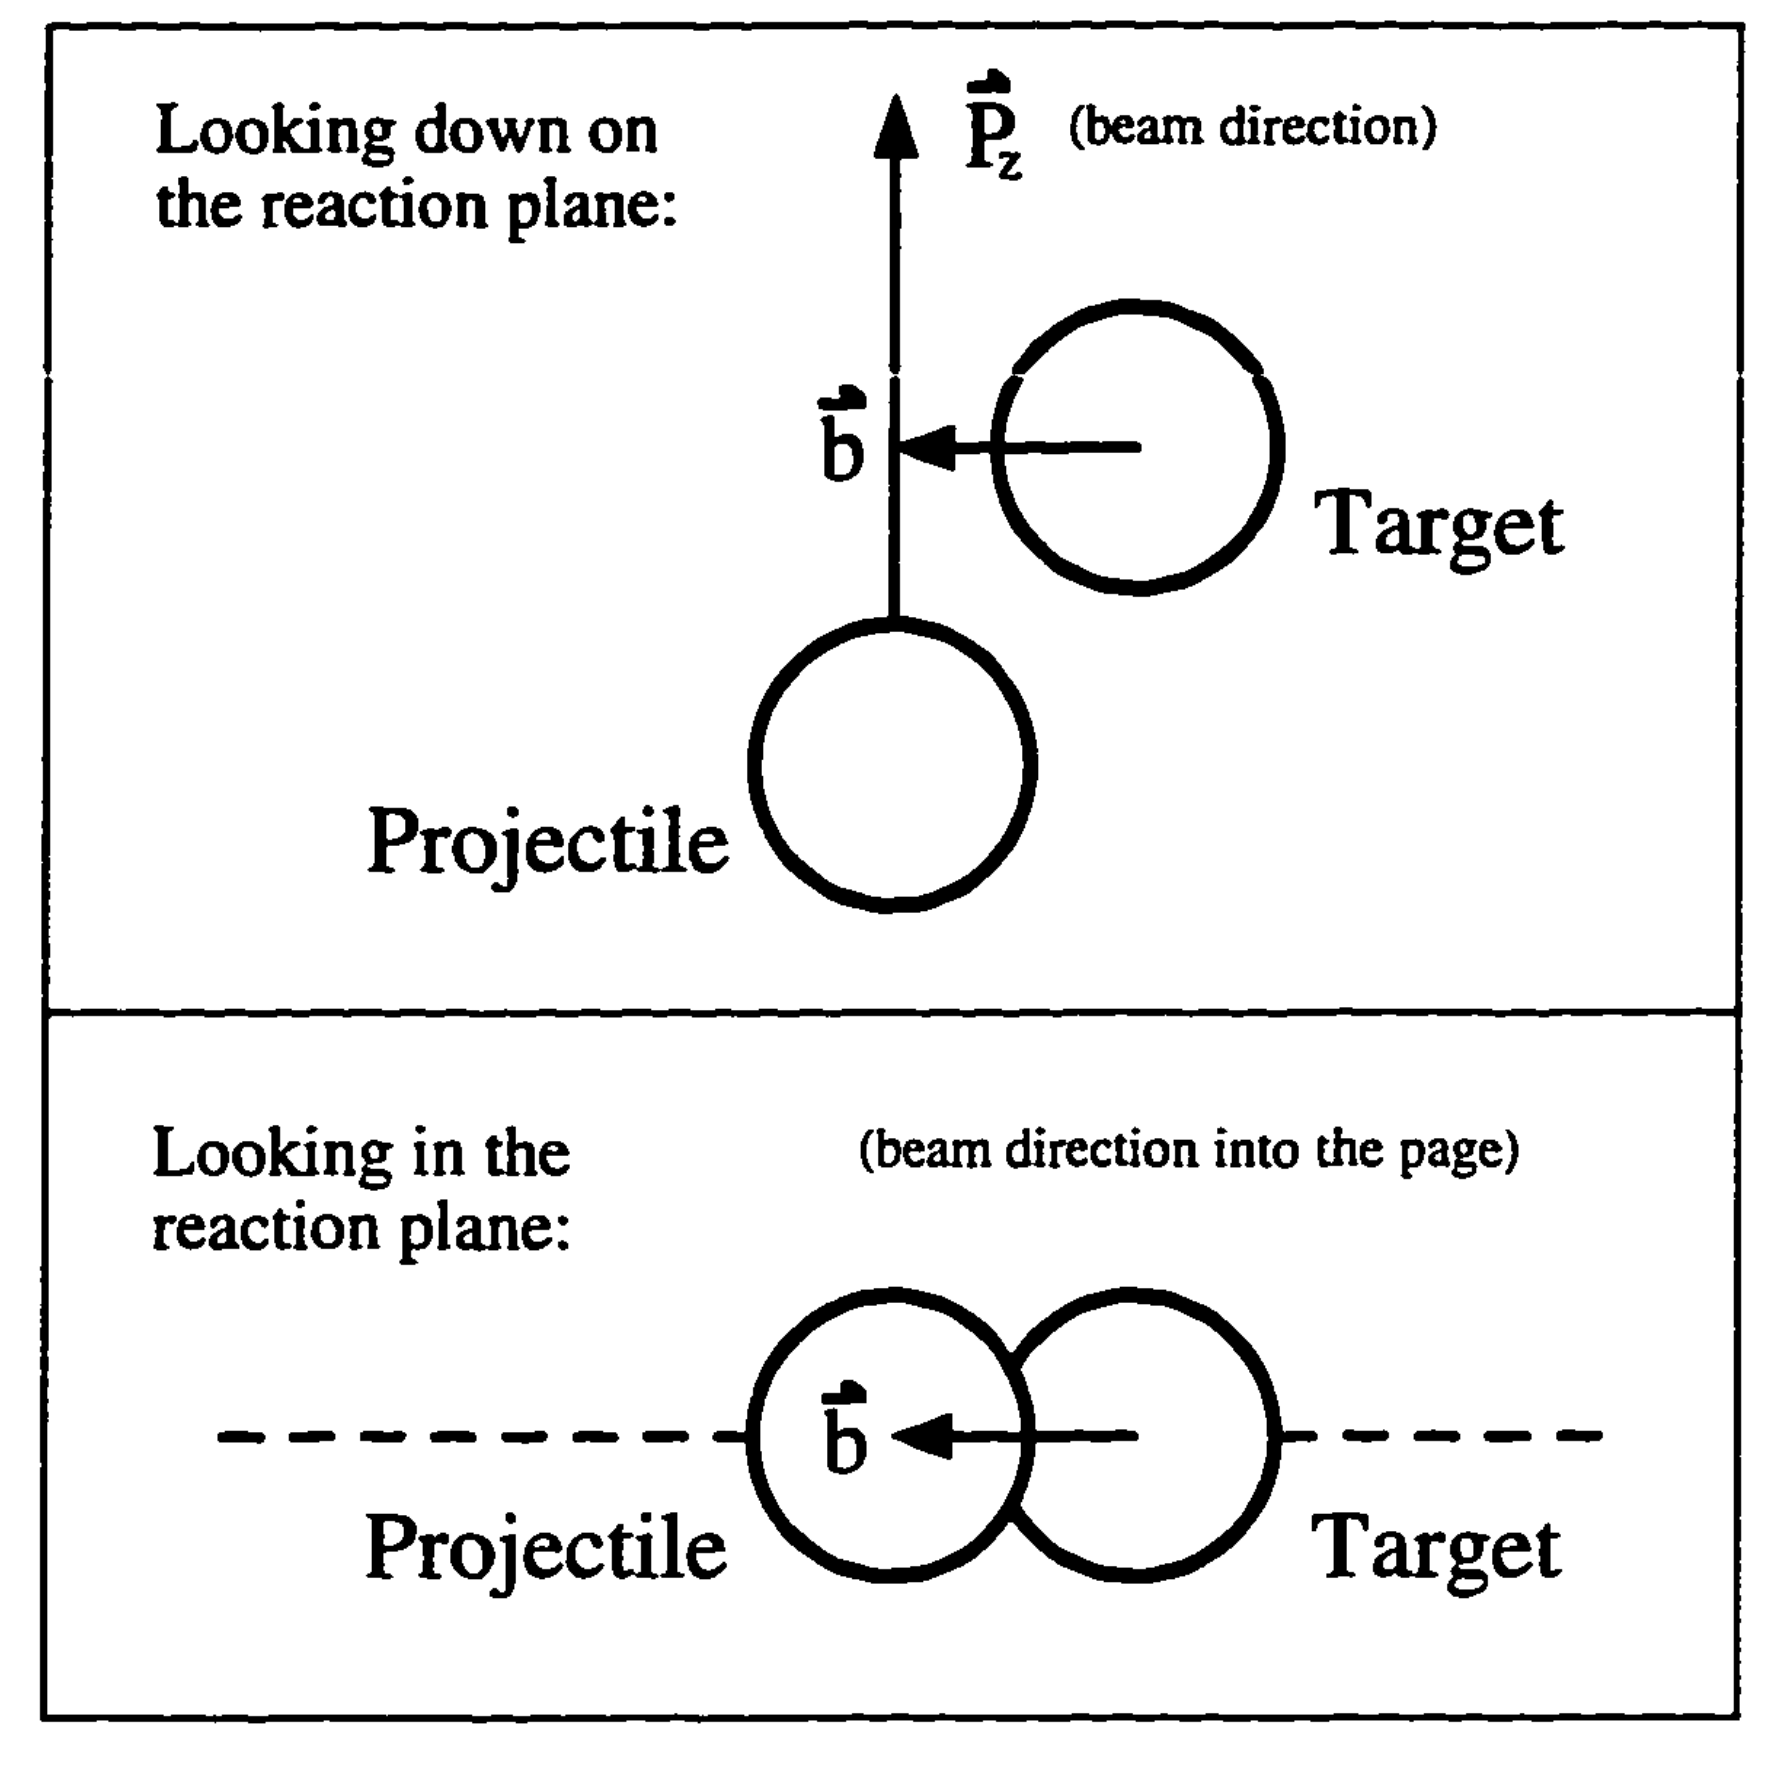
\includegraphics[width=\textwidth]{dad-thesis-figure}               
  One of the figures I helped my dad draw on a computer for his thesis, ``Collective flow in intermediate energy heavy-ion collisions,'' in 1996. Perhaps one day, I too will understand what it means.
\end{marginfigure}

\newthought{To my mother and father}, Dr. Robert and Myung-Hee Pak. My father, who was the first PhD in his own family, whom I remember happily marching down the aisles of the Breslin Center to the honks of Pomp and Circumstance for his doctorate in nuclear physics. Dad, you've been the role model for my life. Ever since I helped draw two figures for your thesis on the Macintosh you got me as a kid, proudly feeling like I had just put the torch on the Statue of Liberty, I've been wondering what it would be like to write one of my own. Well, have I got some bedtime reading material for you! And my mother, who kept me alive and kicking from a single cell all the way to whatever I am today, which if you think about it, is more remarkable than anything you will read in this dissertation. This never could have been written had it not been for my mother's ferocious dedication toward making a better life for me. Thanks, ma!

\newthought{To my thesis advisor}, Dr. Andrew Kasarskis, for taking me under his wing for the past four years. I am supremely lucky to have met somebody with the rare blend of patience, humor, genuine scientific curiosity, and mentorship skills that Andrew has and shares with others so freely. Andrew has taught me more than just science—he has taught me about leadership, entrepreneurship, integrity, life, and occassionally, wildlife. I look forward to pondering his lessons for the rest of my career. And to my fellow Kasarskis brother from the halls of Regis, the inimitable Dr. Joseph R. Scarpa, who blazed a trail for us both and kept me company as we jockeyed desks in Greenland. I am fortunate to be returning to medical school at his side.

\newthought{To the boys of 7G}, who are back in town, spread the word around. Kevin ``Carpet'' Hoffman, Michael ``The Stuffer'' Daniel, Zachary ``BJ'' Lorsch, Eddie ``Other Ted'' Contijoch, and Ranjan ``Gammie'' Upadhyay were my roommates as we began this strange and imprudent quest toward a dual degree. Then there's Andrew T. McKenzie, a late but profitable addition to the gang, who singlehandedly doubled our weirdness quotient and may just achieve his goal of a completely rational life strategy within the decade. And my entire entering class of 2012, who shall be rightfully remembered as ``the Titans.'' We have been through much together: retreats, pyramids, marathons, camping trips, uninhibited human flight, weddings, even a Tough Mudder—many of which could be considered a microcosm of certain aspects of the MSTP experience, but all of which I will always remember. You all kept me variously motivated, alive, and inspired throughout this ignoble quest, and I'll enjoy seeing you all crush it at science, medicine, and life.

\newthought{To the entire Sinai MSTP}, starting with the director from when I entered, Dr. Yasmin Hurd, and the many other leaders that have guided me since: Dr. Margaret Baron, Dr. Talia Swartz, Dr. Benjamin Chen, and Dr. Scott Friedman, to name a few. To the many other students in the program that gave me guidance and support, not least of all Dr. Benjamin Laitman, who was one of the first Sinai students I met, who steadfastly supported me through the challenges of leading Student Council, and whom I am honored to call my friend.

\newthought{To my colleagues in science}, who are also listed in acknowledgements within each chapter, but whom I must thank here not only for their collaborative efforts but also their friendship, mentorship, and personal support. From the Icahn Institute and Department for Genomics and Multiscale Biology: El-Ad David Amir, Oliver Attie, Ali Bashir, Harm van Bakel, Kieran Chacko, Brianne Ciferri, Gintaras Deikus, Gang Fang, Zeynep Gumus, Seunghee Kim-Schulze, Martha Lewis, David Nathanson, Leah C. Newman, Tim O'Donnell, Adeeb Rahman, Eric Schadt, Erick Scott, Robert Sebra, Mayte Suarez-Fariñas, Mitchell Sullivan, Maria Suprun, and Elizabeth Webster. From the Departments of Medicine and Pathology of the Mount Sinai Hospital: Judith Aberg, Camille Hamula, Jonathan Hand, Shirish Huprikar, Gopi Patel, Timothy Sullivan, and Fran Wallach. From the Department of Microbiology of the Icahn School of Medicine at Mount Sinai: Ana Fernandez-Sesma, Rebecca Hamlin, and Irene Ramos-Lopez, aka the Divas of Virology, who were so amazing to work with. To my colleagues from other institutions in the Dengue Human Immune Profiling Consortium, including Eva Harris and Daniela Michlmayr from UC Berkeley and Steven Wolinsky and Eun-Young Kim from Northwestern. There are likely many more scientists that quietly contributed their technical insight and effort to some aspect of the protocols, techniques, and datasets that eventually became a part of this dissertation, and for all of these unsung heroes whom I may never even meet, I want to express my sincere gratitude. 

\newthought{There are many other unsung heroes} in and around Mount Sinai whose support has been invaluable. Firstly, Courtney Manning, Gayle Schneiderman, and Rhaisili Rosario, who all did gangbusters work in keeping the MSTP running. Dr. Rainier P. Soriano, Dr. Yasmin Meah, Dr. David C. Thomas, Paul Lawrence, and Dr. David Muller gave me crucial guidance at certain points in the journey. I was lucky to have advice from Geoffrey Smith and Dan Seltzer on starting my business, The East Harlem Software Company, Inc. I have to thank the staff of Aron Hall, for maintaining such a nice home for all of us students. The guys at El Aguila on 103rd and Lex, whose tortas Cubanas fueled the improbable appearance of many words on these pages (which I recently learned is not an actual food in Cuba, but such is America). No acknowledgements could be complete without saluting Andy Efros, literally the nicest guy at Mount Sinai.

\newthought{I especially want to thank} Dr. Deena Altman for her dedicated leadership and evangelism of the Pathogen Surveillance Program, whose clinical insight and contributions made much of this dissertation possible before I even began, and who supported me from the first day I joined the group. As I go back into the hospital for clerkships and wonder what kind of doctor I want to be, I will be thinking often of Deena.

\newthought{To the members of my thesis advisory committee}: Dr. Adolfo García-Sastre, Dr. Jun Zhu, Dr. Joel Dudley, Dr. Jonathan Karr, and the chair Dr. James Iatridis, for providing focused guidance in developing this dissertation and meticulously supporting my development as a scientist. Special thanks to Dr. Bo Shopsin from the NYU School of Medicine, who graciously agreed to be an outside reviewer. To my undergraduate mentor, Dr. Frederick ``Fritz'' Roth, and members of his laboratory, who supported me throughout and after college, and first inspired me to pursue a doctorate in bioinformatics.

\newthought{Finally, I'd like to thank} Dr. Sonia Yen Jarrett, the only lady brave enough to put up with my shenanigans, who has kept me motivated throughout challenges I once thought impossible, and who always makes me laugh.

%%%%%%%%%%%%%%%%%%%%%%%%%%%%%%%%%%%%%%%%%%%%%%%%%%%%%%%%%%%%%%%%%%%%%%
% -*-latex-*-
  % -*- Mode:TeX -*-
%% This file simply contains the commands that actually generate the table of
%% contents and lists of figures and tables.  You can omit any or all of
%% these files by simply taking out the appropriate command.  For more
%% information on these files, see appendix C.3.3 of the LaTeX manual. 

\tableofcontents
%\newpage
\listoffigures
%\newpage
\listoftables

\cleardoublepage



%%
% We can set the line spacing for the main matter of the document using the toggles below.
% Note that after we do this, we then have to reset spacing between \marginpar's.
\mainmatter
%\doublespacing
\onehalfspacing
\setlength\marginparpush{12pt}
%% A chapter for my PhD dissertation
%% First author: Theodore Pak
%%
%% Must be included from main.tex.

\chapter{Introducing next-generation sequencing and multiscale data analysis into clinical infectious diseases}
\label{chap:intro}

\begin{quote}
\emph{Recent reviews have suggested that routine next-generation sequencing (NGS) on clinical specimens will improve the capabilities of clinical microbiology laboratories. However, the real opportunity to impact our understanding and management of infectious diseases lies in integrating NGS with clinical data from electronic medical records (EMRs), immune profiling data, and other rich datasets to create multiscale predictive models. This chapter introduces a range of new “omics” and patient data sources relevant to infectious diseases and proposes three potentially disruptive applications for these data in the clinical workflow. The combined threats of healthcare-associated infections and multidrug resistant organisms may be addressed by multiscale analysis of NGS and EMR data that is ideally updated and refined over time within each healthcare organization. Such data and analysis should form the cornerstone of future learning health systems for infectious disease.}
\end{quote}

\newthought{Next-generation sequencing} and “big data” analysis techniques are poised to transform our understanding of diseases that have a complex inherited component, such as cancer, diabetes, and heart failure. Perhaps even more significant, however, is the impact these technologies will have on the management of \emph{infectious diseases}, which have discrete, identifiable causes that can be isolated, cultured, and tested against drugs in vitro as part of a standard clinical workflow. Despite steady technological improvements in each step, this workflow’s principles have not changed for a century.\autocite{Didelot2012,Koser2012}

Our capacity to acquire “omics” data about infections is increasing exponentially. Nanoscale parallelization of DNA sequencing has precipitously dropped the cost per base-pair of finished genomes while increasing throughput, and the cost of sequencing and assembling a bacterial genome trends below \$100.\autocite{Didelot2012} PacBio RS sequencing has increased median read lengths over 10kbp, facilitating rapid, automated finishing of genomes for outbreak pathogens.\autocite{Chin2011,Rasko2011} Beyond sequencing pathogen genomes, recent studies have used other “omics” experimental techniques such as Luminex cytokine assays, RNA-seq, and mass cytometry to characterize immune responses to infection or vaccination with remarkable precision.\autocite{Mejias2014,Querec2009}

Many public databases curate and disseminate “omics” data relevant to infectious disease (Table \ref{tab:id_bioinf_dbs}), 
\begin{table*}[ht]
  \centering
  \small
  \begin{tabular}{p{3.5cm} l l l}
    \toprule
    \textbf{Database focus} & \multicolumn{1}{c}{For general research} & \multicolumn{2}{c}{For infectious disease}\\
    \cline{3-4}
    & & \multicolumn{1}{c}{Multi-pathogen} & \multicolumn{1}{c}{Pathogen-specific} \\
    \midrule
    Genomes &
    \begin{minipage}[t]{3.5cm}
      \raggedright
      \begin{itemize}[noitemsep]
      \item NCBI Nucleotide (GenBank/RefSeq)
      \item ENA/EMBL
      \item DDBJ
      \end{itemize}
    \end{minipage} & 
    \begin{minipage}[t]{3.5cm}
      \raggedright
      \begin{itemize}[noitemsep]
      \item ViPR
      \item NMPDR
      \item PATRIC
      \item EuPathDB
      \end{itemize}
    \end{minipage} & 
    \begin{minipage}[t]{3.5cm}
      \raggedright
      \begin{itemize}[noitemsep]
      \item Influenza Research Database (IRD)
      \item Tuberculosis Database (TBDB)
      \item LANL: Databases for HIV, HCV, and HFV 
      \end{itemize}
    \end{minipage}
    \\
    Gene products and functionality &
    \begin{minipage}[t]{3.5cm}
      \raggedright
      \begin{itemize}[noitemsep]
      \item UniProt
      \item KEGG
      \end{itemize}
    \end{minipage} &
    \begin{minipage}[t]{3.5cm}
      \raggedright
      \begin{itemize}[noitemsep]
      \item Pathogen-Host Interaction Database 
      \item Antibiotic Resistance Genes Database
      \item Comprehensive Antibiotic Resistance Database
      \end{itemize}
      \smallskip
    \end{minipage} &
    \\
    Expression and immune profiles &
    \begin{minipage}[t]{3.5cm}
      \raggedright
      \begin{itemize}[noitemsep]
      \item GEO
      \item ArrayExpress
      \end{itemize}
    \end{minipage} &
    \begin{minipage}[t]{3.5cm}
      \raggedright
      \begin{itemize}[noitemsep]
      \item ImmPort
      \end{itemize}
    \end{minipage} &
    \\
    \bottomrule
  \end{tabular}
  \caption[Bioinformatics databases for infectious diseases][12pt]{Examples of public bioinformatics databases that may be leveraged for multiscale analysis of infectious disease (this list is not exhaustive).}
  \label{tab:id_bioinf_dbs}
\end{table*}
but most lack significant clinical metadata. Increasing adoption of electronic medical records (EMRs) can potentially mitigate this problem because they typically include data on demographics, medications, lab results, and more. Figure \ref{fig:emr_sample_viz} presents a visualization of some of these datatypes as recorded by Mount Sinai Hospital’s EMR for two patients diagnosed with \textit{C. difficile} colitis.
\begin{figure}[htb]
  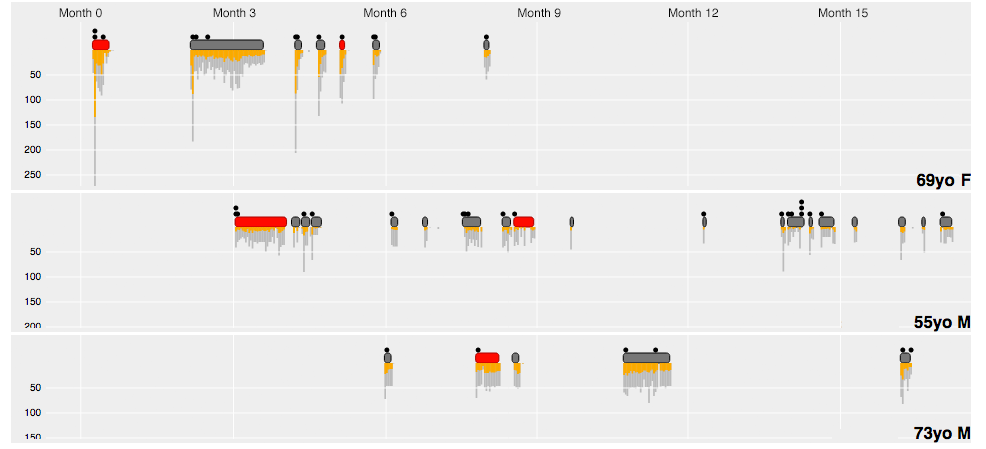
\includegraphics[width=\textwidth]{chap1/pt-timelines-deidentified}               
  \caption[Visualization of EMR data]{\textbf{Visualization of EMR data.} Timelines for two patients generated from EMR data in the Mount Sinai Data Warehouse (original analysis). Patient visits to Mount Sinai are represented as horizontal bars across the top of the timeline, and visits associated with a \textit{C. difficile} infection are highlighted in red.  The number of lab tests ordered per day is represented on the vertical axis, with abnormal results highlighted in orange.  Transfer events are marked by the black dots above the horizontal bars.}
  \label{fig:emr_sample_viz}
\end{figure}
With so many different stakeholders entering EMR data, however, automatically extracting certain facts (e.g., “this patient had the flu last Tuesday”) can be difficult. Nevertheless, high-accuracy methods for extracting infectious phenotypes such as influenza-like illness \sidecite[-1.2cm]{Silva2013}, unclear HIV status,\autocite{Felsen2014} and community-acquired pneumonia\autocite{DeLisle2013} have been demonstrated, and consortia such as eMERGE are standardizing comparison, validation, and deposition of these algorithms into a central repository.\autocite{Pathak2013a}

The marriage of real-time digital clinical information with “omics” technology creates the opportunity to increase the precision of clinical decision-making and challenges us to quickly design and execute bioinformatics analyses. Predictive modeling of infectious disease that incorporates EMR data is still rare, although one recent study generated a social network for hospital acquired infection from EMR data using recorded contacts between patients and caretakers.\autocite{Cusumano-Towner2013} Another found that statistical analysis of EMR data produces risk factors for C. difficile infection that outperform models based only on medically recognized risks.\autocite{Wiens2014} Likely because of the difficulty of integrating data across so many levels, no published studies have yet bridged predictive modeling on EMR data with pathogen genome sequences or other “omics” data from individual patients. Yet, for infectious disease, this is exactly what will fulfill the vision of a rapid-learning health system \autocite{Care2014,Kohane2012} that converts the informational byproducts of healthcare recorded by practitioners into evidence for future decision-making. While EMR data holds details of the clinical process and outcomes, “omics” data ties it back to pathophysiology and the precise strain and host-pathogen interactions present in each patient. Together, they can fuel a “learning engine” that integrates heterogeneous data into new clinical insights, interventions, and therapies. We will discuss how to leverage current bioinformatics software to build such an engine, and how this engine will be able to attack currently insurmountable problems in the field.

\section{The genomic clinical microbiology laboratory}

\newthought{Previous reviews}\autocite{Didelot2012,Koser2012} have proposed that cheap sequencing technology will transform clinical microbiology, while acknowledging technical and informational barriers to adoption. Whole genome sequencing (WGS) via NGS provides ultimate resolution for epidemiological studies of transmission and relatedness, and may soon be cost-effective for routine use.\autocite{Didelot2012,Koser2012} For pathogen identification, however, NGS is unlikely to usurp robotic culturing systems (e.g., Vitek and BD Phoenix) or newer mass spectrometry systems by cost and sensitivity comparisons alone, although it can lower turnaround time for difficult-to-culture organisms and identify novel or rarely-seen pathogens.\autocite{Koser2012,Naccache2015} Since susceptibility or resistance of an organism to drugs is in principle fully encoded in its genetic material \autocite{Didelot2012,Gordon2014}, NGS can also lower turnaround times for drug susceptibility testing of slow-growing organisms, such as M. tuberculosis \autocite{Boehme2010} and HIV-1.\autocite{Ram2015} This strategy should only expand as fuller catalogs of genomic variants that cause drug resistance are compiled for other pathogenic organisms.

\subsection{Leveraging existing bioinformatics tools}

An oft-mentioned hurdle\autocite{Didelot2012,Koser2012} for widespread use of NGS in clinical microbiology is the lack of readily accessible software for converting these data into species identifications, phylogenies, and drug susceptibilities. However, many mature open source bioinformatics solutions for individual components of these problems exist, and connecting these components into a pipeline is therefore a tractable software engineering exercise. Examples for most subtasks are listed in Table \ref{tab:id_bioinf_tools}. As NGS use by clinical microbiology laboratories becomes more commonplace, we might anticipate full-fledged genomic clinical microbiology software packages to become widely available.

\newthought{This expectation} has three foreseeable shortcomings. The first is that current tools are tied to centrally curated repositories of evidence. Although proponents of genomic clinical microbiology often envision encyclopedic databases hosted by international consortia,\autocite{Didelot2012,Koser2012} human curation is expensive and inefficient at scale, and many infectious diseases are locale-specific phenomena. Models based on pooled data may fail to reflect variation between healthcare delivery regions;\autocite{Reis2003,Wiens2014} for instance, a recent fitness model of H3N2 influenza based on international genomic surveillance data creates predictions only at the resolution of clades spanning multiple continents.\autocite{Luksza2014} Since implementation of NGS in a healthcare institution’s microbiology laboratory produces copious sequencing data not easily shared through public databases, institutions should prepare to manage repositories of local evidence and predictive models that work specifically for them. Over time, as data exchange interfaces are developed, institutions could form consortia to generalize analyses, which is a strategy that has successfully increased the power of human genome-wide association studies.\sidecite[-3em]{Gottesman2013,Kohane2012}

\begin{table}[ht]
  \centering
  \small
  \begin{tabular}{l l}
    \toprule
    \textbf{Problem domain} & \textbf{Software or database}\\
    \midrule
    Strain typing &
    \begin{minipage}[t]{5cm}
      \raggedright
      \begin{itemize}[noitemsep]
      \item Multi-Locus Sequence Typing (MLST) database
      \end{itemize}
      \smallskip
    \end{minipage}
    \\
    \textit{De novo} assembly from long reads &
    \begin{minipage}[t]{5cm}
      \raggedright
      \begin{itemize}[noitemsep]
      \item Celera
      \item Hierarchical Genome Assembly Process
      \end{itemize}
    \end{minipage}
    \\
    Species identification &
    \\
    \-\tabindent From clonal sample &
    \begin{minipage}[t]{5cm}
      \raggedright
      \begin{itemize}[noitemsep]
      \item NCBI BLAST
      \item GenBank
      \item Other databases in Table \ref{tab:id_bioinf_dbs}
      \end{itemize}
    \end{minipage}
    \\
    \-\tabindent From non-clonal sample &
    \\
    \-\tabindent\tabindent  Meta-assembly &
    \begin{minipage}[t]{5cm}
      \raggedright
      \begin{itemize}[noitemsep]
      \item AMOS
      \item MIRA
      \item MetaVelvet
      \end{itemize}
      \smallskip
    \end{minipage}
    \\
    \-\tabindent\tabindent Clustering and species annotation &
    \begin{minipage}[t]{5cm}
      \raggedright
      \begin{itemize}[noitemsep]
      \item MEGAN
      \item MG-RAST
      \end{itemize}
      \smallskip
    \end{minipage}
    \\
    Maximum likelihood phylogeny trees &
    \begin{minipage}[t]{5cm}
      \raggedright
      \begin{itemize}[noitemsep]
      \item BEAST
      \item RAxML
      \item ClonalFrame
      \item ClonalOrigin
      \end{itemize}
      \smallskip
    \end{minipage}
    \\
    Whole genome alignment &
    \\
    \-\tabindent For SNP calling &
    \begin{minipage}[t]{5cm}
      \raggedright
      \begin{itemize}[noitemsep]
      \item Mummer
      \item Mugsy
      \item Harvest
      \end{itemize}
      \smallskip
    \end{minipage}
    \\
    \-\tabindent For structural variant calling &
    \begin{minipage}[t]{5cm}
      \raggedright
      \begin{itemize}[noitemsep]
      \item Mauve
      \end{itemize}
      \smallskip
    \end{minipage}
    \\
    Gene annotation &
    \\
    \-\tabindent Bacterial &
    \begin{minipage}[t]{5cm}
      \raggedright
      \begin{itemize}[noitemsep]
      \item Glimmer
      \item RAST
      \item prokka
      \end{itemize}
      \smallskip
    \end{minipage}
    \\
    \-\tabindent Drug resistance in bacteria &
    \begin{minipage}[t]{5cm}
      \raggedright
      \begin{itemize}[noitemsep]
      \item Resfinder
      \item ARG-ANNOT
      \item Mykrobe predictor
      \end{itemize}
      \smallskip
    \end{minipage}
    \\
    \-\tabindent Other &
    \begin{minipage}[t]{5cm}
      \raggedright
      \begin{itemize}[noitemsep]
      \item Influenza Virus Sequence Annotation Tool
      \end{itemize}
      \smallskip
    \end{minipage}
    \\
    \bottomrule
  \end{tabular}
  \caption[Bioinformatics tools for infectious diseases]{Selected published bioinformatics software packages or databases that address specific steps of clinical microbiology tasks using NGS data (this list is not exhaustive). Well-established tools are available for many specific subtasks.}
  \label{tab:id_bioinf_tools}
\end{table}

A second shortcoming is that current pathogen annotation tools primarily make predictions using the simplistic criterion of sequence similarity. Machine learning (ML) algorithms could eventually integrate a wider array of genotypic features extractable from pathogen genomes—variant calls, putative gene and motif annotations, and more—and train holistic models that predict phenotypes. A “top-down,” integrative model predicting limited phenotypes from genotype for Mycoplasma genitalium is available;\autocite{Karr2012} top-down predictions of virulence, however, add the substantial complexity of host interactions. Therefore, genome-wide ML models of virulence have mostly been “bottom-up,” blind to mechanistic knowledge, and oriented toward even smaller-genome pathogens with considerable genomic surveillance data. ML on viral sequence features has predicted more effective antiretroviral combinations for HIV,\autocite{Lengauer2006,Zazzi2012} genetic markers for host selectivity within families of viruses,\autocite{Raj2011a} and optimal strain selection for H3N2 influenza vaccines.\autocite{Luksza2014} In general, given the explosion in available data, significant untapped potential remains for ML-based models that predict virulence, transmissibility, and drug resistance from pathogen genotypes. 

The third shortcoming is that for many common pathogens, these models are still limited by the paucity of clinical metadata linked to sequenced pathogens. Pathogen phenotypes accessible directly from EMRs include prognostic variables, such as length of stay and disposition, and lab results, such as drug susceptibilities. Although lab information systems (LIS) typically do not forward non-clinical results (e.g., growth curves) to EMRs, data exported from the LIS can help define richer phenotypes. For some diseases, EMRs will contain lab results that directly reflect infection severity, e.g., viral load for HCV and HIV patients,\autocite{Norton2014} while other diseases will require more complex criteria.\autocite{DeLisle2013,Klompas2008,Silva2013} Natural language processing of physician notes will facilitate the extraction of complex, high-accuracy clinical phenotypes from the EMR.\autocite{Liao2015,Silva2013} Routine NGS of specimens and EMR data on drugs prescribed and administered will enable ad-hoc studies crossing pathogen genotypes against interventions and outcomes. Richer characterization of particular host-pathogen encounters may be provided by immune and molecular profiling of selected patients, as well as animal experiments that establish individual pathogen genetic associations and molecular mechanisms. Biomarkers derived from such data\autocite{Mejias2014,Querec2009} could enhance predictive models built on a zealous integration of NGS and EMR data.

\newthought{The growth of EMR} phenotype information associated with pathogen genomes will spur a new generation of pathogenicity and risk models based on genomic data. Ideally, these models can drive a “learning engine” that integrates heterogeneous input data from an encounter with an infected patient and predict outcomes for possible interventions. Predictions can be delivered to physicians via clinical decision support systems that complement EMR functions by suggesting relevant actions within a patient’s electronic chart. The closing of the EMR–NGS–EMR loop (Figure \ref{fig:emr_ngs_loop}) should be the ultimate goal of bioinformatics pipelines for genomic clinical microbiology, because this would maximize the utility of data created for clinical encounters, continuously turning yesterday’s observations and outcomes into evidence for tomorrow’s predictions.\sidecite[-2em]{Care2014,Kohane2012}

\begin{figure}[htb]
  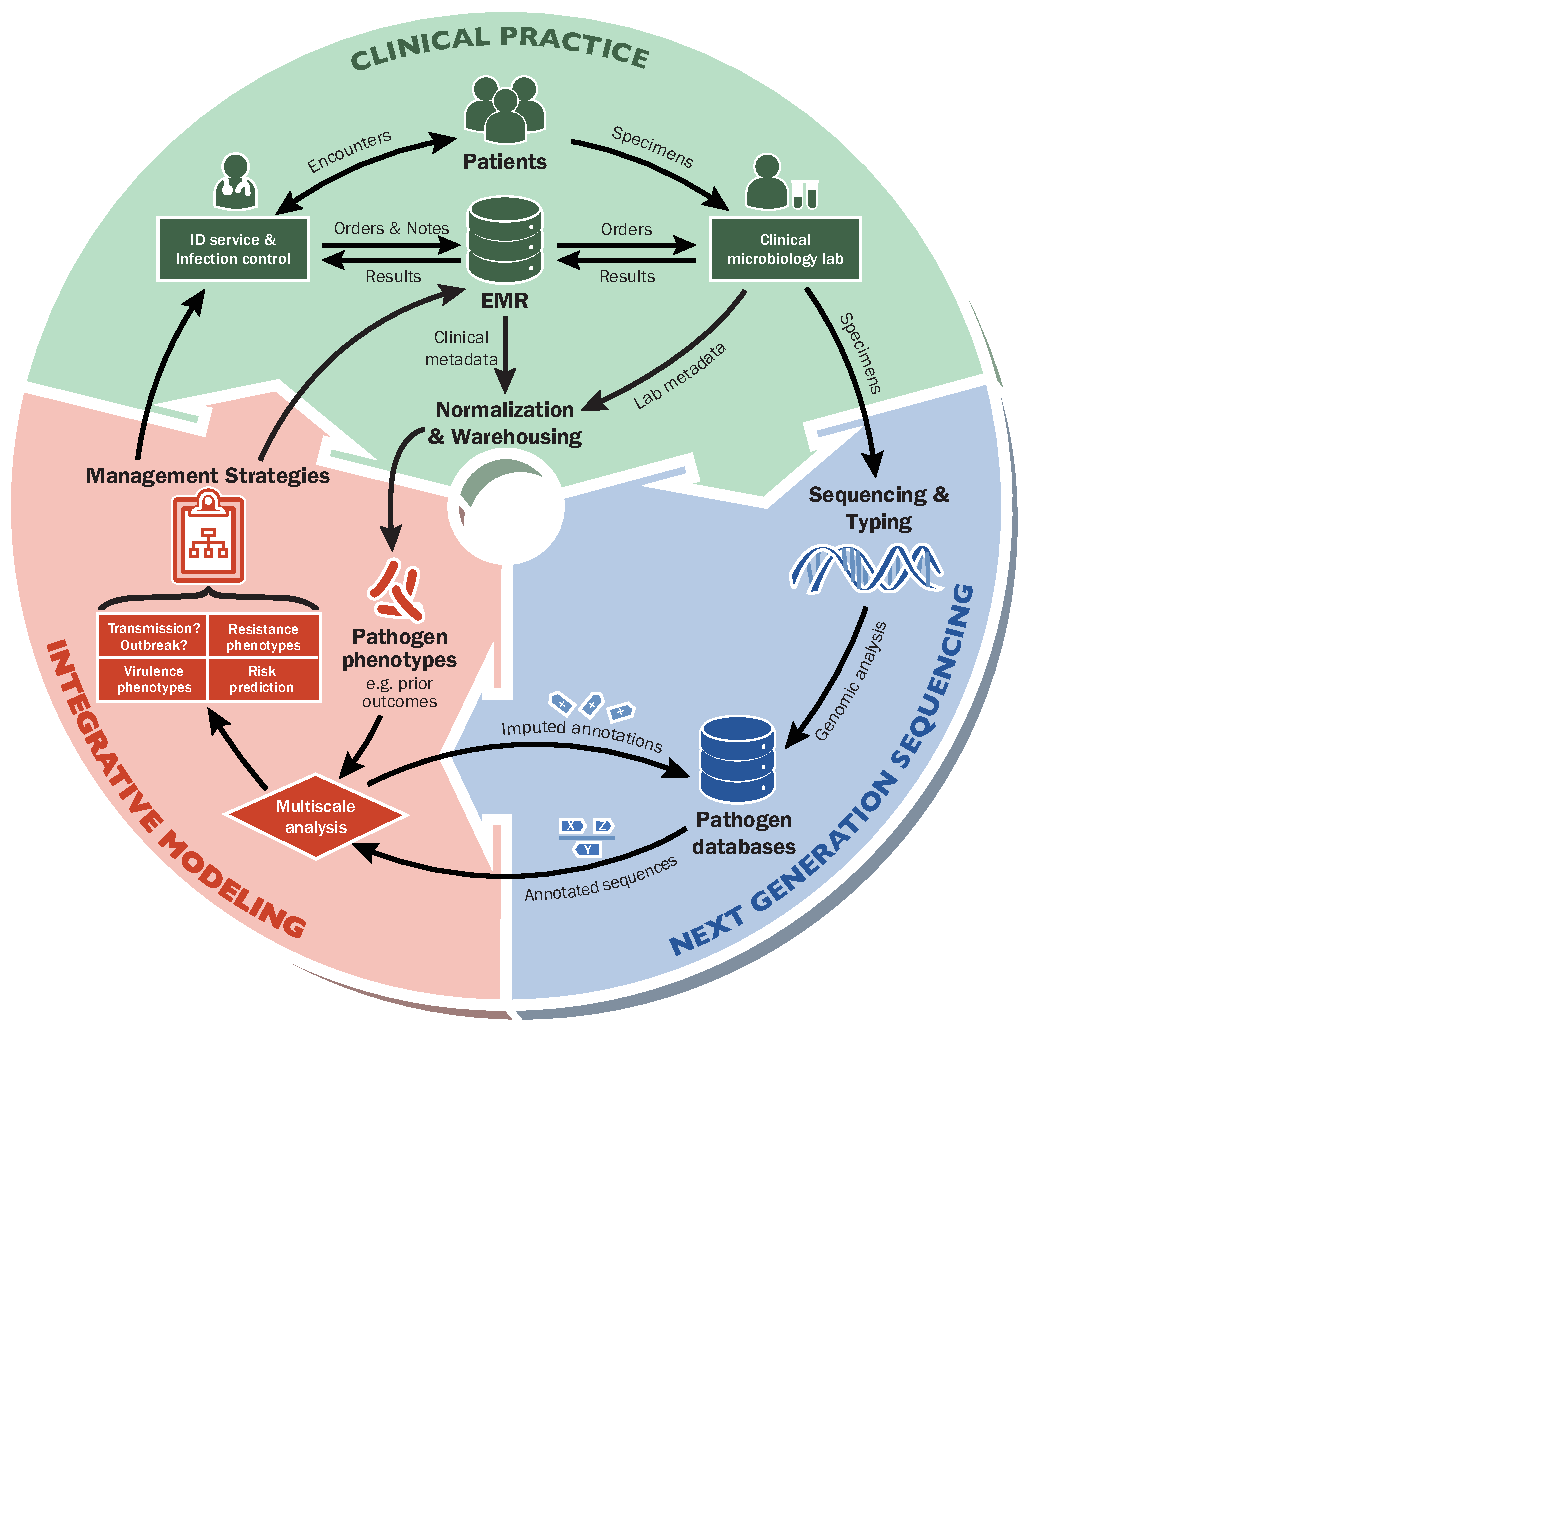
\includegraphics[width=\textwidth]{chap1/emr-ngs_loop_circular}               
  \caption[A learning health system for infectious diseases]{\textbf{A learning health system for infectious diseases.} Next generation sequencing (NGS) technologies now permit routine genomic analysis of clinical microbiology specimens. When integrated with pathogen phenotypes derived from clinical metadata in electronic medical records (EMRs) and laboratory metadata, we can generate predictive models for pathogen transmission, outbreaks, drug resistance, virulence, and risk factors for infection or critical outcomes that are specific to the health system and its patient population. If management strategies are formulated from these predictions and sent to infectious disease (ID) physicians and hospital infection control, a continuous loop of data analysis, application, and model refinement is created.}
  \label{fig:emr_ngs_loop}
\end{figure}

This sounds ambitious, but we can look to analogous software designed as subcomponents of learning healthcare systems to anticipate likely costs and avenues for development. The i2b2 platform\autocite{Kohane2012} and its counterpart SCILHS\autocite{Mandl2014} are vendor-agnostic solutions for extracting and unifying data across EMRs for reuse in cohort design and robust meta-analysis. The eMERGE consortium stimulated the creation of SHARPn for normalization and natural language processing of EMR data\autocite{Rea2012} and CLIPMERGE for automated pharmacogenomics alerts.\autocite{Gottesman2013} For these examples, working software was created after 1-5 years of development with \$100k-\$10M of annual public grant funding.\autocite{Gottesman2013,Kohane2012,Mandl2014,Rea2012} If the aforementioned open-source software is leveraged, an equal scale of public funding and collaboration among academic medical centers could make similar strides toward the proposal in Figure \ref{fig:emr_ngs_loop}. A modular framework allowed i2b2 to expand in scope organically after initial release,\autocite{Kohane2012,Mandl2014} suggesting that successful strategies should first aim for simple but clinically useful tasks such as identifying species and transmissions while anticipating the addition of more complex analyses via plugins and community contributions. In short, a reasonable investment in scrupulous software engineering could produce the seeds of a learning health system for infectious disease within the decade.

\section{Beyond genomic data}

\newthought{While NGS rapidly} moves toward routine use by clinical microbiology laboratories where it can be integrated with EMR data, other advances in data collection on infectious diseases create significant opportunities for predictive modeling that may eventually impact clinical practice. We now review these additional sources of data.

\subsection{Immune profiling}

Host response to infection is not merely the result of single gene modulations or amplification of specific cell types, but rather consists of complex interacting networks of RNA transcription, protein signaling and metabolism that impact cellular, tissue, and whole organism behaviors. The nature of the modulations that are specific to the host’s particular system relative to the state of the system at the time of infection ultimately determines risk and severity of disease. Recent studies have used “omics” scale experimental techniques to provide groundbreaking insight into immune responses, ranging from classification of acute respiratory infections in children\autocite{Mejias2014} and predicting immunogenicity of a vaccine\autocite{Querec2009,Furman2013} to characterizing effects of aging that gradually decrease vaccine efficacy.\autocite{Poland2014}

In each of these studies, researchers took an unbiased, hypothesis-free approach to their design and observed as many properties of the immune system as was experimentally feasible before, during, and after a perturbation, such as vaccine administration. Such properties include cytokine levels as measured by Luminex assays, global changes in gene expression within various leukocyte populations as measured by RNA-seq or microarrays, and changes in cell populations with various surface markers as observed by flow and mass cytometry. With sufficient sample size, patterns of biomarkers can be linked to various clinical outcomes, e.g., the host becoming immunogenic to an antigen. These biomarkers can then be investigated further for their functional role or used in new assays for point-of-care diagnosis. For common presenting conditions, like acute febrile illness, where current diagnostic methods poorly distinguish between bacterial and viral disease, this capability would allow prompt selection of the most appropriate therapy.\autocite{Mejias2014} For diseases like dengue that do not have accurate markers of immunization, these markers will be essential for development of a successful vaccine.\autocite{Mahalingam2013}

\subsection{The internet}

\begin{figure}[htb]
  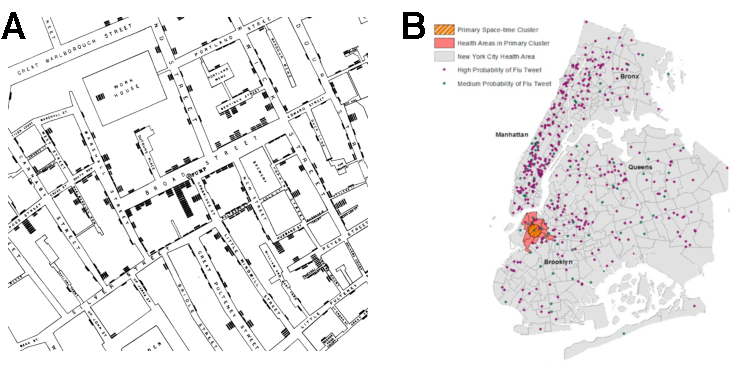
\includegraphics[width=\textwidth]{chap1/snow_and_new_combined}               
  \caption[Geospatial analysis, then and now]{\textbf{Geospatial analysis, then and now}. A, Excerpt from a map published by John Snow in 1855 depicting a cluster of cholera cases around a water pump on Broad Street in London, England. B, Retrospective analysis of geocoded tweets in New York City classified by the probability of representing actual influenza cases during the 2012-2013 flu season, from \textcite{Nagar2014}. The primary outbreak cluster was determined to be in Northern Brooklyn.}
  \label{fig:snow_and_new_combined}
\end{figure}

Patients can now be associated with a trove of digitized information that can be mined to better understand infectious disease. Frequent social contacts are often captured in address books, email inboxes, and social networks like Facebook. Patients discuss symptoms online, which have been captured from search engine queries\autocite{Ginsberg2009} or public Twitter streams to find probable cases of pertussis, whooping cough, and influenza,\autocite{Nagel2013} although these studies have known limitations.\autocite{Lazer2014} Often this data is attached to geospatial information, which can be used to construct spatiotemporal models of the disease that reveal clusters and the directionality  of spread within a city environment,\autocite{Nagar2014} providing in real time the same type of analysis that 19th century anesthesiologist John Snow meticulously compiled to identify a London water pump handle as the source of a cholera outbreak (see Figure \ref{fig:snow_and_new_combined}).\autocite{Buechner2004,Snow1855} Global human movement patterns are also captured in air travel network usage data, which has previously been combined with genomic surveillance data to predict transmission dynamics of H3N2 influenza.\autocite{Lemey2014} Unifying such diverse data in clinically relevant models with actionable outputs remains a significant challenge. On the other hand, the advent of cloud computing and open-source data science platforms like Apache Hadoop, used by Facebook and Walmart to model complex consumer behavior, suggests that algorithms for large, heterogeneous datasets will become increasingly accessible to healthcare providers and life sciences researchers.\autocite{Mohammed2014}

\section{Impact on clinical management}

\newthought{Three potential applications} of a new learning healthcare system for infectious diseases could address some of the most urgent global problems in infectious disease. One problem is rising antimicrobial resistance, which the World Health Organization names one of the three greatest threats to human health.\autocite{Policy2010} Care providers overusing antimicrobials and fomenting resistance in subclinical carriers are partly to blame, with recent studies estimating the fraction of misuse to be between quarter to half of all treatments.\autocite{McKellar2014} Multidrug resistance increases the morbidity and mortality of healthcare-acquired infections (HAIs), which have an incidence of 1.7 million cases per year in the US and an estimated annual cost of more than \$30 billion \autocite{Scott2009} that dwarfs the likely cost of any informatics-based preventative efforts. The sobering threat of extensively drug-resistant community-circulating organisms, some of which have therapeutic failure rates of 25-29\%,\autocite{Hirsch2010} alters the risk analysis for hospital procedures once considered routine and calls for comprehensive new strategies for management.

\subsection{Identifying high-risk patients for HAI}

Infection control for HAIs depends on identifying high-risk patients and applying isolation precautions or reducing known risk factors during their hospital course. For C. difficile infection (CDI), the most frequently reported nosocomial infection in the US, many questions about how infections are acquired and managing at-risk patients remain.\autocite{Leffler2015} The prevailing notion that infections are mostly transmitted person-to-person within hospitals \autocite{Cohen2010} conflicts with recent NGS evidence that sources of infection are more diverse,\autocite{Eyre2013} suggesting a greater role for asymptomatic colonized patients and environmental sources.

Each healthcare system represents a unique milieu of person-to-person contact networks, contaminated surfaces, microbiomes, and asymptomatic colonization that contributes to the risk of CDI. EMR and NGS data can prove or disprove transmission between patients and unlock the secrets of modifiable risk factors in this chaotic environment. ML algorithms predicting individual risk of CDI for a large hospital performed better (area under receiver operator curve, AUC=0.81) when operating on >10,000 unconstrained EMR variables rather than curated variables for known risk factors.\autocite{Wiens2014} Similar ML models based on EMR data between 2009-2014 for The Mount Sinai Hospital in New York City, encompassing 192,000 patients and 1,366 CDI diagnoses, show equal performance (AUC=0.80) and draw out associations not typically published for CDI. These may be unique to Mount Sinai’s environment and include respiratory failure (odds ratio OR=8.3, 95\% confidence interval 6.6-10.3), nutritional irregularity (OR=6.6, 4.7-8.6), and pancytopenia (OR=4.4, 3.1-5.5) (Timothy O’Donnell, personal communication).

A model-based decision support system would screen patients with higher CDI or asymptomatic colonization likelihood and allow earlier diagnosis and intervention. NGS-confirmed transmission events and interactions between people and equipment seen in the EMR and other data could extend this basic model to highlight common factors behind verified transmission and inform empirical, real-time modifications of infection control policy. Cross-sectional analysis by NGS-derived phenotypes and risk factors in the EMR would facilitate more precise clinical decision-making, for instance, whether shortening patient time in intensive care units or decreasing use of provocative antibiotics would be more preventative within the local milieu.  Short of a clinical trial that is probably infeasible to conduct, much less replicate across institutions, there is scant evidence for making these decisions at present, so a localized quantitative model can only help.

\subsection{Earlier detection of outbreaks inside and outside the hospital}

Current infection control software suites like VigiLanz Dynamic Monitoring Suite and TheraDoc Infection Control Assistant primarily issue outbreak alerts based on infection frequency thresholds. This could be rendered obsolete by routine NGS of clinical microbiology specimens, which determines with great precision whether a transmission event has occurred.\autocite{Didelot2012,Koser2012} A software system with access to EMR and other hospital data could automatically search elements common between verified transmission cases (caregivers, equipment, or rooms) and alert staff to inspect these elements before they produce enough transmissions to trigger a frequency threshold alert. Given enough historical data, NGS could also help hospitals differentiate community- from hospital-acquired infections and thereby refine metrics used to evaluate infection control policies.

An active effort to sample the environment inside and outside the hospital could further extend the reach of this surveillance. Within the hospital, “problem spots” identified by earlier investigations could be resampled regularly via NGS to re-evaluate the efficacy of infection control measures. The hospital also samples the pathogen ecosystem of the local population. Hospitals already report diagnoses of highly transmissible and dangerous infections to government authorities, and sharing NGS data for these cases would permit real-time assessment of where pathogens are coming from, how they are evolving, and where populations naïve to a pathogen are located. Current mapping and surveillance efforts \autocite{Brownstein2008} would be vastly enhanced by rich phylogenetic information, allowing outbreaks across disparate regions to be linked.\autocite{Chin2011,McAdam2012,Rasko2011} Fine-grained, real-time tracking of infectious disease spread would better inform doctors diagnosing and treating new patients, field agents tracking cases and contacts, and health policymakers seeking preventive population measures.

\subsection{Antimicrobial stewardship}

Decision support systems for empirical antibiotic therapy have been investigated for decades,\autocite{Leibovici1997} but with the prevalence of antimicrobial resistance skyrocketing, the urgency to implement systems that specifically encourage restraint with antibiotics has increased.\autocite{Wagner2014} Selective reporting is a common strategy that directs providers toward optimal therapies simply by omitting names of inappropriate drugs in susceptibility reports.\autocite{Doern2013} A more aggressive strategy pushes EMR alerts whenever physicians prescribe antibiotic treatment inconsistent with best practices.\autocite{Kullar2013}

These solutions ignore the power of the EMR to provide evidence that justifies or improves the antimicrobial stewardship interventions. For instance, although it is well accepted that antibiotic overuse increases the prevalence of resistance, current antimicrobial stewardship programs have demonstrated neither effects on patient outcomes nor even that decreased antibiotic treatment leads to decreased antibiotic resistance.\autocite{Wagner2014} By integrating NGS and EMR data, these hypotheses could be investigated in minute detail within large patient cohorts. NGS can reveal and enumerate the genetic mechanisms of resistance circulating through a health system. By tracing the recurrence of pathogens in the local community, an NGS-equipped health system can determine whether patients receiving antibiotics have generated and transmitted drug-resistant mutants. Specific drug regimens can be correlated with the development of particular resistance mutations. Conversely, given enough longitudinal data, the efforts of an antimicrobial stewardship program can be validated by observing decreased emergence of resistance mutations to drugs prescribed more conservatively.

\section{Conclusions}

\newthought{Routine access} to pathogen genomic data will transform our ability to manage infections, but only if we can integrate this information with clinical and other data to power predictive models for critical outcomes. Assuming that the hurdles of cost, accuracy, and turnaround time can be addressed, which is likely given current trends, NGS will soon become a standard clinical microbiology procedure. The unprecedented specificity of this data will in the near term allow reconstruction of transmission networks inside and outside of hospitals. In the far term, having rich clinical data linked to pathogen genotypes will permit predictions of prognosis, virulence, and drug susceptibility for active infections once NGS data is available. Incorporating these capabilities into a new clinical workflow that actively refines predictive models by adjusting to new data (Figure \ref{fig:emr_ngs_loop}) should improve case management, risk prediction for HAIs, detection of outbreaks, and antimicrobial stewardship. The missing link in this transformation, and the goal for bringing it to fruition, is software that leverages best-of-breed existing tools, incorporates all relevant heterogeneous datatypes, builds on electronic phenotyping algorithms to scrub low-accuracy EMR data, and validates against gold standard clinical case review.
Healthcare institutions and researchers should recognize that a potent combination of NGS and EMR data will transform infectious disease management. The threats posed by multidrug resistance and healthcare associated infections demand a revolution in management strategy. Predictive modeling grounded in rich, diverse molecular and clinical data will dramatically increase the precision of care and help hold these threats at bay.

\section*{Notes}

A shortened version of this chapter was published in \textit{Clinical Infectious Diseases}.\autocite{Pak2015}

\subsection{Acknowledgements}

We thank Deena Altman and Shirish Huprikar for critical suggestions on the manuscript.

\subsection{Financial support}

The authors were supported by the Icahn Institute for Genomics and Multiscale Biology at Mount Sinai.

\subsection{Potential conflicts of interest}
We certify no potential conflicts of interest.

%% This is an example first chapter.  You should put chapter/appendix that you
%% write into a separate file, and add a line \include{yourfilename} to
%% main.tex, where `yourfilename.tex' is the name of the chapter/appendix file.
%% You can process specific files by typing their names in at the 
%% \files=
%% prompt when you run the file main.tex through LaTeX.

\chapter{Whole-genome sequencing identifies emergence of a quinolone resistance mutation in a case of \emph{Stenotrophomonas maltophilia} bacteremia}
\label{chap:steno}

\begin{quote}
\emph{In this chapter we use next-generation sequencing to reveal the mechanism of emerging drug resistance in a case of hospital-acquired infection following the failure of routine antimicrobial therapy. Whole genome sequences for \emph{Stenotrophomonas maltophilia} serial isolates from a bacteremic patient before and after development of levofloxacin resistance were assembled \emph{de novo} and differed by one single-nucleotide variant in \emph{smeT}, a repressor for multidrug efflux operon \emph{smeDEF}. Along with sequenced isolates from five contemporaneous cases, they displayed considerable diversity compared against all previously published complete genomes. Whole genome sequencing and complete assembly can conclusively identify resistance mechanisms emerging in \emph{S. maltophilia} strains during clinical therapy.}
\end{quote}

\section{Introduction}

\emph{Stenotrophomonas maltophilia} is an aerobic, non-fermenting, and motile Gram-negative bacterium that is increasingly recognized as a cause of hospital-acquired infections with crude mortality rates of 14–69\% in cases of bacteremia.\autocite{Brooke2012} Treatment of \emph{S. maltophilia} infections is challenging due to the pathogen’s intrinsic resistance to many antibiotic classes via drug efflux pumps, beta-lactamase production, and decreased membrane permeability.\autocite{Brooke2012} Resistance phenotypes are known to change during the course of treatment, which complicates interpretation of automated drug susceptibility testing (DST) results.\autocite{Garrison1996} A mutant strain of \emph{S. maltophilia} with emerging resistance to tetracycline, chloramphenicol, and quinolones was previously characterized following in vitro tetracycline selection.\autocite{Alonso1997,Sanchez2002} However, little is known about the genetic and molecular mechanisms underlying acquired resistance in the clinical setting—particularly for quinolones, where in contrast to other Gram-negatives, the quinolone-resistance determining region (QRDR) of topoisomerase genes is often unaltered.\autocite{Valdezate2005} In this report, we describe the first reported use of whole genome sequencing (WGS) in serial clinical isolates to definitively identify an acquired quinolone resistance mutation in \emph{S. maltophilia}. WGS was performed for the initial and subsequent \emph{S. maltophilia} blood culture isolates from a patient where acquired quinolone resistance was observed (Patient 1) and five other patients (Patients 2-6) selected from a two-month period in 2013 at The Mount Sinai Hospital. 

\section{Case report}

Patient 1 was a 56 year-old man with a history of pancreatic cancer and a Whipple procedure eleven years earlier who presented to The Mount Sinai Hospital with variceal bleeding at the hepaticojejunostomy site. A transjugular intrahepatic portosystemic shunt was placed, which was complicated by thrombosis. In the following weeks, he had several episodes of polymicrobial bacteremia and was treated with multiple courses of antimicrobials, including a 10-day course of levofloxacin. Two months after levofloxacin exposure, he developed another episode of polymicrobial bacteremia. Blood cultures intermittently grew \emph{S. maltophilia}, \emph{E. faecium}, and \emph{Candida parapsilosis} despite appropriate antimicrobial therapy. Automated DST showed that the first \emph{S. maltophilia} isolate acquired was susceptible to levofloxacin (minimum inhibitory concentration [MIC] 0.5µg/mL) and trimethoprim/sulfamethoxazole (TMP-SMX; MIC ≤20 µg/mL). He was treated with 400 mg intravenous ciprofloxacin every 8 hours, but blood cultures nine days later again grew \emph{S. maltophilia}, now resistant to levofloxacin (MIC >32µg/mL) while still susceptible to TMP-SMX (MIC 1µg/mL). Ciprofloxacin therapy was stopped and intravenous TMP-SMX was given every 8 hours; subsequent cultures did not grow \emph{S. maltophilia}.

\section{Methods}

Standard culturing and susceptibility testing for levofloxacin and SXT were performed by automated microbroth dilution with Vitek2® (bioMérieux). Antimicrobial sensitivities were reported and interpreted according to the 2015 CLSI guidelines for \emph{S. maltophilia}.\autocite{ClinicalandLaboratoryStandardsInstitute2015} Isolates were then stocked and frozen at -80°C. Levofloxacin and SXT susceptibilities for all isolates in this study were later confirmed by Etest (bioMérieux) at 24 hours. To prepare for sequencing, isolates were grown from single colonies in tryptic soy broth, and DNA extraction was performed as previously described.\autocite{Altman2014}

\subsection{Genome sequencing}

Sequencing was performed to a depth of coverage of >150x per genome using the P4-C2 sequencing enzyme and chemistry at the manufacturer’s specifications on the PacBio RSII platform (Pacific Biosciences, Menlo Park, CA). For ISMMS2 and ISMMS2R, Sanger sequencing was additionally performed on six PCR-amplified regions encompassing the one single nucleotide variant (SNV) and five one-base indels that differentiated the two PacBio assemblies. Conventional PCR amplification was performed with Choice-Taq Blue (Denville Scientific) and included an initial denaturation step of 180s at 95°C, 30 cycles of denaturation, annealing, and extension at 95°C/30s, 60°C/30s, and 72°C/30s respectively, and a final extension step of 300s at 72°C. Primer sequences are as follows: for the SNV, \texttt{5’-CAAGGTGCTGACCGAAATGC-3’} forward and \texttt{5’-ACACGCCATCCTTCACGTAG-3’} reverse; and for the five indels, \texttt{5’-GCATGGAAGTACCACTGGGT-3’} forward + \texttt{5’-TTGGAGGGGTGGTAAAACGG-3’} reverse, \texttt{5’-TGGCCAACCCCTTCTATGTC-3’} forward + \texttt{5’-CCATGGCCACAGCAAAATGG-3’} reverse, \texttt{5’-CTGCCTTCGGTCACTTCGT-3’} forward + \texttt{5’-TGGAAGTCTCGCTGGAAGGT-3’} reverse, \texttt{5’-GCCCTCTACACCGTCTTTCC-3’} forward + \texttt{5’-GAACTACCGGACGGCTTTGA-3’} reverse, and \texttt{5’-AACTTCTTCGTGTCGGTCCC-3’} forward + \texttt{5’-AGAACTACCGGACGGCTTTG-3’} reverse. Sequences on both strands of the amplified products were determined at an external sequencing facility (Macrogen Inc., Rockville, MD) using the standard Sanger dideoxy-terminator method and the same primers.

\subsection{Sequence assembly and annotation}

Sequencing data was processed and assembled de novo using PacBio’s Hierarchical Genome Assembly Process\autocite{Chin2013} (HGAP, version 3) in the SMRTanalysis toolkit (version 2.3.0) using standard pre-assembly pipeline parameters. Custom scripts were used to circularize the draft assemblies and orient them similarly to reference assemblies K279a, R551-3, D457, and JV3 using the \emph{gyrB} locus as a landmark; these scripts are available at \url{https://github.com/powerpak/pathogendb-pipeline/releases/tag/steno\_v1.0} (\textsc{doi}:\href{http://dx.doi.org/10.5281/zenodo.17295}{10.5281/zenodo.17295}) within the files \texttt{scripts/circularizeContigs.pl} and \texttt{scripts/fasta-orient-to-landmark.pl}. To eliminate overhanging sequence at the end of contigs and to increase accuracy, raw reads were re-mapped to the circularized assemblies using Blasr and the final consensus was re-called using Quiver. Initial annotations were created using the RAST server\autocite{Overbeek2014} with specific annotation of sme genes derived from BLAST queries.
Depth of coverage reported in Table 1 was calculated by SMRTanalysis (version 2.3.0) during re-mapping of reads to the circularized draft assembly.

\subsection{Accession numbers}

Sequences and annotations for reference assemblies of clinical \emph{S. maltophilia} isolates K279a, R551-3, D457, and JV3 were obtained from GenBank/RefSeq at accession numbers \texttt{AM743169.1}, \texttt{NC\_011071.1}, \texttt{NC\_017671.1}, and \texttt{NC\_015947.1}, respectively. These represent the entirety of assemblies for \emph{S. maltophilia} found in NCBI Assembly with an Assembly Level of “Complete Genome” (\url{http://www.ncbi.nlm.nih.gov/assembly/organism/40324/all/}) at the time of the study.\footnote{By 2017, excepting the three assemblies submitted as a result of this study, only one more complete genome (\href{https://www.ncbi.nlm.nih.gov/assembly/GCF\_002025605.1/}{ASM202560v1}) is available.} K279a and D457 were isolated from human infections, while R551-3 and JV3 were isolated from plants. Previously published sequences for the quinolone-resistance determining region (QRDR) of the \emph{gyrA}, \emph{gyrB}, \emph{parC} and \emph{parE} genes in \emph{S. maltophilia}\autocite{Valdezate2002} were obtained from EMBL/European Nucleotide Archive.

Complete genome sequences for ISMMS2, ISMMS2R, and ISMMS3 were deposited in GenBank at accession numbers \texttt{CP011305}, \texttt{CP011306}, and \texttt{CP011010}, respectively. Deposited sequences for ISMMS2 and ISMMS2R incorporate the Sanger corrected regions described above. Sequences for ISMMS4, ISMMS5, ISMMS6, and ISMMS7 were deposited as Whole Genome Shotgun projects at DDBJ/EMBL/GenBank under the accessions \texttt{JZIU00000000}, \texttt{JZIV00000000}, \texttt{JZIW00000000}, and \texttt{JZTX00000000}, respectively, with the versions described in this chapter at \texttt{JZIU01000000}, \texttt{JZIV01000000}, \texttt{JZIW01000000}, and \texttt{JZTX01000000}, respectively.

\subsection{Comparative genomic analysis}

Pairwise comparison between strains was performed with the MUMmer 3.23 package,\autocite{Delcher2003} firstly using nucmer for pairwise genome alignment. The resulting nucmer alignments were filtered for quality and uniqueness via the \texttt{delta-filter} tool (using the \texttt{–1} flag to identify top alignments between the reference and query intervals). To estimate phylogenetic tree distances, high-quality SNP and indel calls were assigned via the \texttt{show-SNPs} tool using the \texttt{–C} flag to only report SNPs in regions with unambiguous mappings. For ISMMS2 and ISMMS2R, \texttt{show-SNPs} was also used without the \texttt{–C} flag to verify that no additional SNPs or indels were in ambiguously mapped regions.

Mugsy version 2.2 was used to perform multiple sequence alignment of the whole genome sequences in order to find local collinear blocks (LCBs) of conserved sequence.\autocite{Angiuoli2011} These aligned blocks were used to establish a core genome (of 3.01 Mbp) across all isolates, from which a phylogenetic tree was constructed using RAxML version 8.0.2,\autocite{Stamatakis2014} employing the GTRGAMMA substitution model and performing 20 runs. Whole genome alignments for visualization of recombination events was performed with Mauve 2.4.0,\autocite{Darling2004} using the \emph{progressiveMauve} algorithm\autocite{Darling2010} with a minimum seed weight of 21, seed families enabled, and all other parameters at defaults. Clustal Omega\autocite{Sievers2011} was used for multiple sequence alignment of putative amino acid sequences, which were then rendered with ESPript version 3.0.\autocite{Robert2014}

\subsection{Epigenetic motif analysis}

For each isolate, initial DNA modification motifs were first predicted by a de novo motif discovery pipeline in SMRTportal (\texttt{RS\_Modifications\_Motif\_Analysis.1}). The pipeline searches for kinetic variations in DNA polymerization events recorded during sequencing that correlate with modifications in the template, with different modifications creating distinct kinetic profiles.\autocite{Clark2012,Fang2012} At the coverage depths reported for this study, the probability (power) of detecting a modification event at a site at the 0.1 significance threshold, if it is truly modified, exceeds 99.99\%.\autocite{Fang2012} Raw predictions, which often have incorrectly- or over-called motifs, were further refined by a re-analysis of the raw data using a single molecule level characterization method.\autocite{Beaulaurier2015} Conceptually, this method was used to check the single molecule level methylation status of each putative motif and its neighboring (more or less specific) motifs and determine the real motif. 

\section{Results}

Two complete whole genome sequences were derived from Patient 1’s isolates before and after the change in levofloxacin MIC and compared to whole genome sequences of five control \emph{S. maltophilia} isolates (Patients 2-6). All sequences were \emph{de novo} assembled, i.e., without regard to reference assemblies. Table \ref{tab:steno_pts} summarizes the relative dates of collection, antimicrobial susceptibility results, and assembly statistics.

\newcommand{\PreserveBackslash}[1]{\let\temp=\\#1\let\\=\temp}
\newcolumntype{P}[1]{>{\PreserveBackslash\raggedright}p{#1}}

\begin{table*}[ht]
  \centering
  \small
  \begin{flushleft}
  \begin{tabular}{l P{1.5cm} P{1.5cm} l l l l P{2.5cm} P{1.5cm}}
    \toprule
    \multirow{2}{*}{Patient} & 
    \multirow{2}{1.5cm}{Time of collection (days)$^a$} &
    \multirow{2}{1.5cm}{Isolate name} &
    \multicolumn{2}{P{3cm}}{Levo susceptibility (MIC, mg/L)} &
    \multicolumn{2}{P{3cm}}{SXT susceptibility (MIC, mg/L)} &
    \multirow{2}{2.5cm}{Assembly quality} &
    \multirow{2}{1.5cm}{Depth of coverage}
    \\
    \cmidrule(r){4-5}\cmidrule(r){6-7}
    & & & Vitek2 & Etest & Vitek2 & Etest & &
    \\
    \midrule
    1  &  0   & ISMMS2  &  S (0.5)$^b$ &  S (1)     & S (<20)      & S (0.19) & 1 circular 4.51Mbp chromosome & 160x \\
    1  &  +10 & ISMMS2R &  R (>32)$^b$ &  R (16)    & S (1)        & S (0.38) & 1 circular 4.51Mbp chromosome & 403x \\
    2  &  -26 & ISMMS3  &  S (0.25)  &  S (0.38)  & U (80, <20)$^c$ & S (0.75) & 1 circular 4.80Mbp chromosome & 153x \\
    3  &  +14 & ISMMS4  &  R (>8)    &  R (>12)   & U (0.5, 80)$^c$ & S (0.75) & 3 contigs (4.73Mbp, 6.5kbp, 11.2kbp) & 303x \\
    4  &  -32 & ISMMS5  &  S (1)     &  S (1)     & S (<20)      & S (0.25) & 18 contigs & 270x\\
    5  &  0   & ISMMS6  &  S (<0.12) &  S (0.125) & S (<20)      & S (1.5)  & 10 contigs & 262x\\
    6  &  +2  & ISMMS7  &  S (1)     &  S (0.75)  & S (<20)      & S (1.5)  & 1 circular 4.69Mbp chromosome, 1 additional 17.7kbp contig & 318x\\
    \bottomrule
  \end{tabular}
  \end{flushleft}
  \caption[Sequenced clinical isolates and their antimicrobial susceptibilities]{Sequenced clinical isolates and their antimicrobial susceptibilities. Abbreviations: Levo, levofloxacin; SXT, trimethoprim/sulfamethoxazole; S, susceptible; R, resistant; U, undetermined; Mbp, million base pairs; kbp, thousand base pairs. $^a$Time of collection was defined in days relative to the date of collecting the initial \emph{S. maltophilia} isolate in the case patient. $^b$This is the change in levofloxacin susceptibility investigated in this study. $^c$Inconsistent results were obtained in replicate.}
  \label{tab:steno_pts}
\end{table*}

\subsection{Emergence of a point mutation conferring quinolone resistance}

Assembled genome sequences for Patient 1’s isolates before (ISMMS2) and after (ISMMS2R) observation of levofloxacin resistance were compared directly and were identical except for one single-nucleotide variant (SNV) and five one-base indels. Sanger sequencing confirmed the presence of the SNV, but identified the indels as homopolymer assembly errors. Coding domain sequence predictions for the surrounding locus (Figure \ref{fig:snp_location}A) revealed that the SNV was inside \emph{smeT}, a \emph{tetR}-like repressor upstream of the structural operon for the \emph{smeDEF} genes, which encode a multidrug efflux pump. The SNV is an A>T substitution at position 497 of \emph{smeT} causing a nonsynonymous Leu-166→Gln mutation.

\begin{figure*}[tbp]
  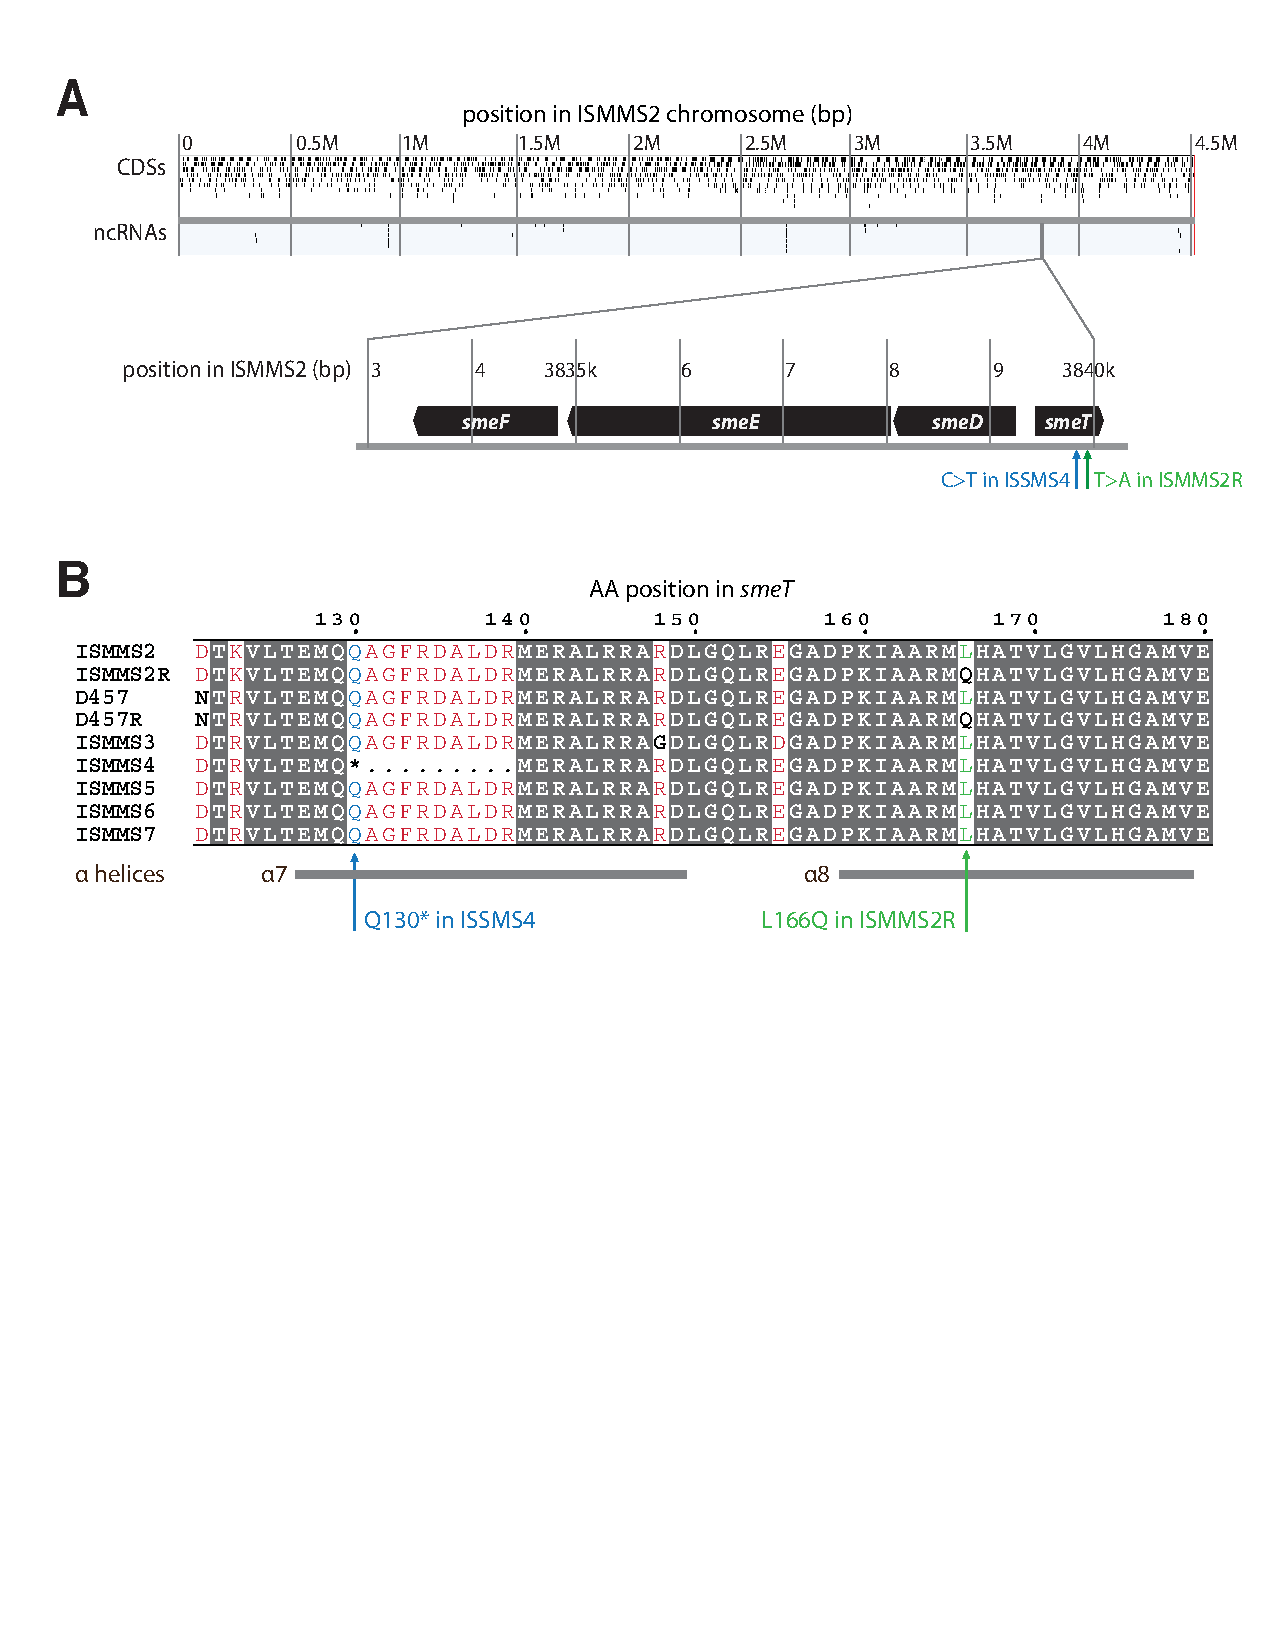
\includegraphics[width=\textwidth]{chap2/snp_location}
  \fullwidthlabelcaption{fig:snp_location}{SNVs observed in quinolone-resistant \emph{S. maltophilia} clinical isolates.}{
    \textbf{Single-nucleotide variants (SNVs) observed in quinolone-resistant \emph{S. maltophilia} clinical isolates.} A, assembled circular chromosome for ISMMS2, including predicted coding domain sequence (CDS) and noncoding RNA (ncRNA) features drawn with ChromoZoom. Horizontal position corresponds to base pair location. The \emph{smeDEF} operon is shown in the detail callout, which highlights both the \emph{smeT} c.497T>A SNV that emerged in ISMMS2R and the aligned location of the \emph{smeT} c.388C>T SNV (encoding a premature stop codon) in ISMMS4. ISMMS2 and ISMMS2R are serial isolates from a single patient before and after development of quinolone resistance, while ISMMS4 was quinolone-resistant at initial isolation from a different patient. B, multiple sequence alignment of part of the predicted \emph{smeT} product in each of the clinical isolates, the D457 reference assembly, and its quinolone resistant counterpart D457R. Predicted α-helices are labeled as grey bars below the sequence. Positions identical in all sequences are shaded with a dark gray background, equivalent substitutions are typeset in red, and non-equivalent substitutions are typeset in boldface black. The L166Q and Q130* (*, stop codon) polymorphisms are highlighted.
  }
\end{figure*}

The same nonsynonymous mutation has been previously observed in an in vitro strain of \emph{S. maltophilia}, D457R, created by selecting single-step tetracycline-resistant mutants from the antibiotic-susceptible clinical strain D457 \autocite{Alonso1997,Sanchez2002}. The mutation is in the eighth α-helix of the \emph{smeT} protein \autocite{Hernandez2009}, which homodimerizes to repress transcription of the \emph{smeDEF} operon \autocite{Hernandez2009,Sanchez2002}. Although the mutation is not in the DNA-binding region, it has been shown to disable the repressor activity of \emph{SmeT},\autocite{Sanchez2002} leading to upregulation of \emph{SmeDEF} and conferring an MDR phenotype \autocite{Alonso2001}.

Figure \ref{fig:snp_location}B shows an amino-acid sequence alignment comparing \emph{SmeT} in D457 and D457R to aligned sequences from our seven isolates. Notably, while none of the remaining isolates shared the same Leu-166→Gln (c.497A>T) mutation, another isolate resistant to levofloxacin, ISMMS4, displayed a C>T mutation at position 388 of \emph{smeT} that creates a premature stop codon that likely disrupts \emph{smeT} function (Figure \ref{fig:snp_location}A and \ref{fig:snp_location}B).

\begin{figure}[htb]
  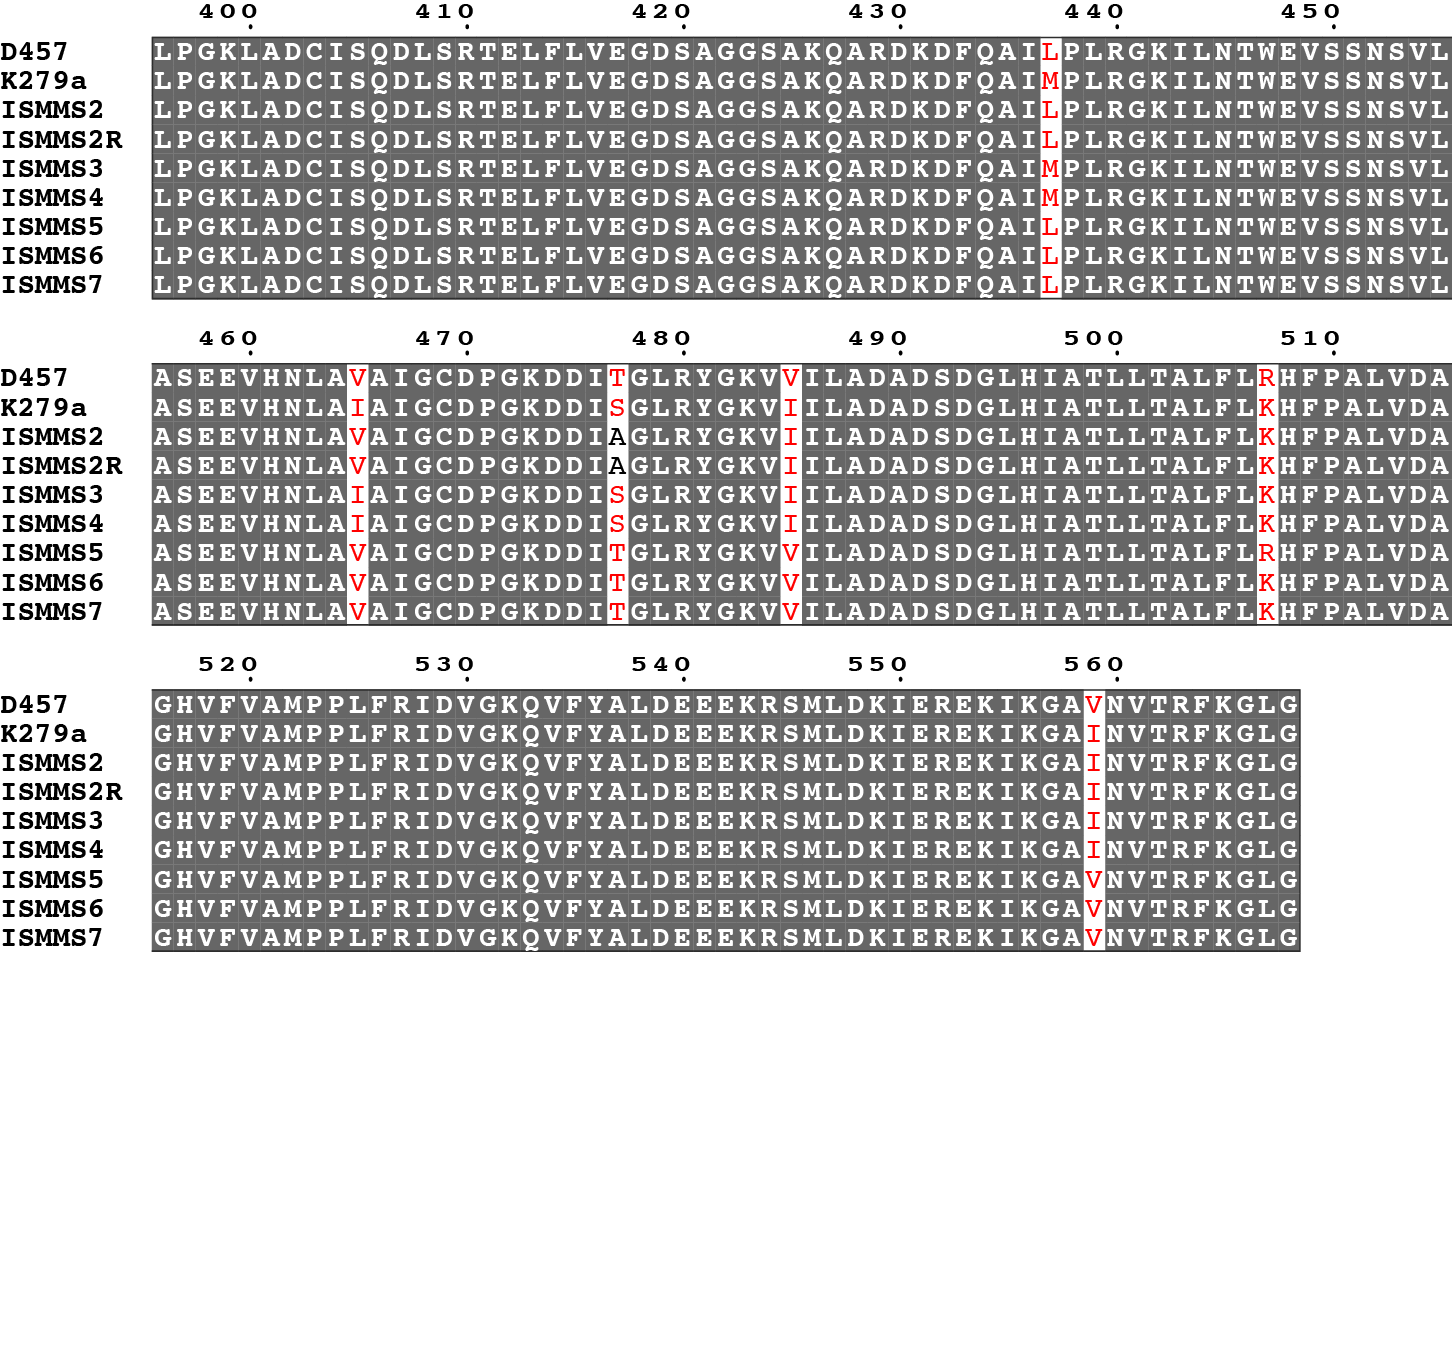
\includegraphics[width=\textwidth]{chap2/qrdr_locus}               
  \caption[Amino-acid sequence alignment for the quinolone-resistance determining region (QRDR) of the \emph{parE} gene]{Amino-acid sequence alignment for the quinolone-resistance determining region (QRDR) of the \emph{parE} gene for seven S. maltophilia clinical isolates (ISMMS2 through 7 and ISMMS2R) and two reference assemblies of clinical isolates obtained from GenBank.}
  \label{fig:qrdr_locus}
\end{figure}
 
The QRDR are loci within genes encoding topoisomerase II and IV subunits known for mutations that confer quinolone resistance in Gram-negative bacteria, although they appear to play a secondary role to efflux systems for resistance emerging during treatment of \emph{S. maltophilia} infection.\autocite{Valdezate2005} An amino-acid sequence alignment of the \emph{gyrA}, \emph{gyrB}, and \emph{parC} genes of our seven isolates and the reference clinical isolates D457 and K279a revealed no differences in the QRDR. Some variants were observed within the QRDR of \emph{parE} (Figure \ref{fig:qrdr_locus}), all of which were consistent with past observations in clinical isolates \autocite{Valdezate2002} except for an Ile-599→Val variant observed in three of our isolates and the D457 reference sequence.

\subsection{Diverse sources of \emph{S. maltophilia} identified with WGS}

Significant genomic diversity was observed among the \emph{S. maltophilia} isolates from all six patients. Figure \ref{fig:steno_phylo} shows a maximum-likelihood phylogeny with branch lengths scaled to SNV distances. Our isolates distribute widely among all four reference assemblies for complete \emph{S. maltophilia} genomes in GenBank. The distances of tens of thousands of SNVs seen in our phylogeny suggest that the natural diversity of pathogenic \emph{S. maltophilia} is greater than that captured by the current set of reference assemblies, even within a single hospital setting. 

\begin{figure}[htb]
  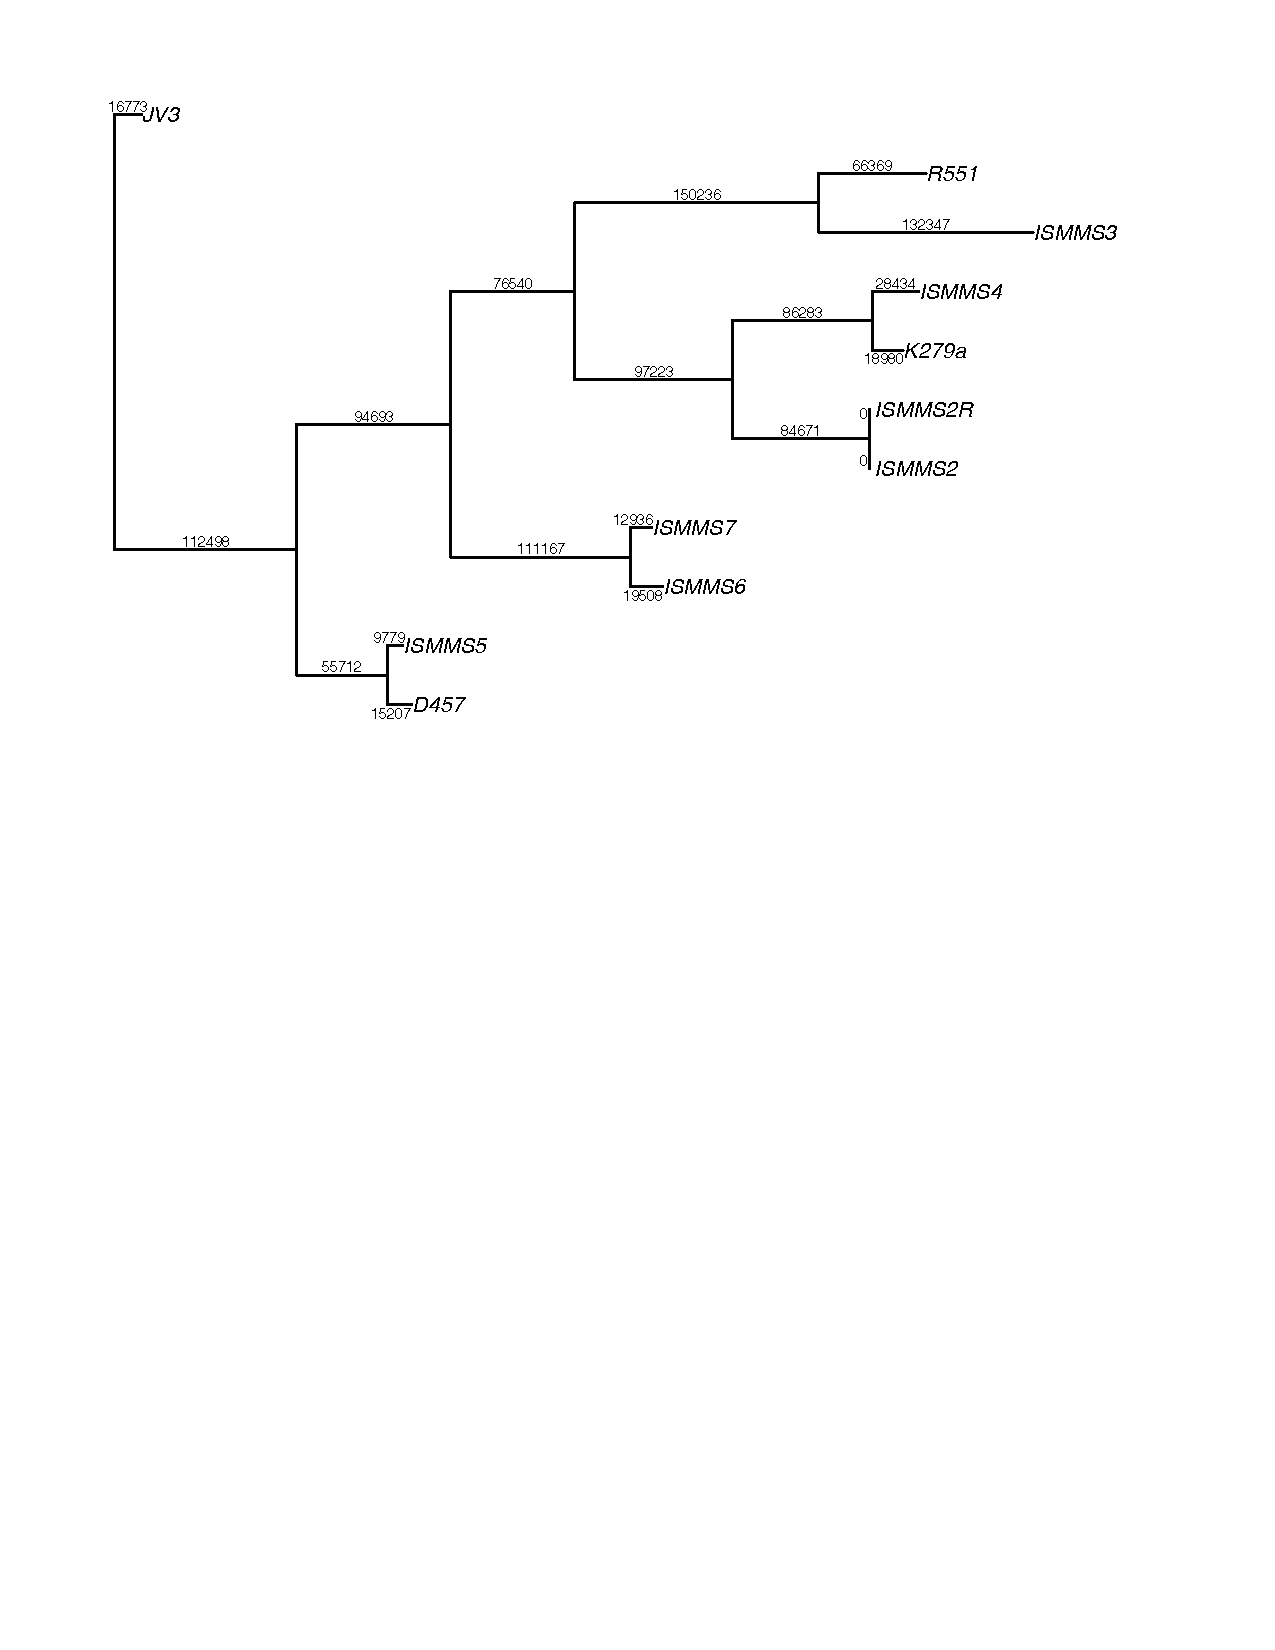
\includegraphics[width=\textwidth]{chap2/phylogram}               
  \caption[Phylogeny of seven \emph{S. maltophilia} clinical isolates]{Phylogeny of seven \emph{S. maltophilia} clinical isolates (ISMMS2 through 7 and ISMMS2R) and four reference assemblies obtained from GenBank. Trees were constructed by inferring ancestral states using RAxML-8.0.2; branch lengths correspond to single-nucleotide polymorphism (SNP) distances from branch points, and are drawn using R version 3.0.3 and the APE library version 3.1-1. The core genome did not contain the \emph{smeT} locus; therefore, the SNV differentiating ISSMS2 and ISMMSR is not observed in this tree.}
  \label{fig:steno_phylo}
\end{figure}

\begin{figure}[htb]
  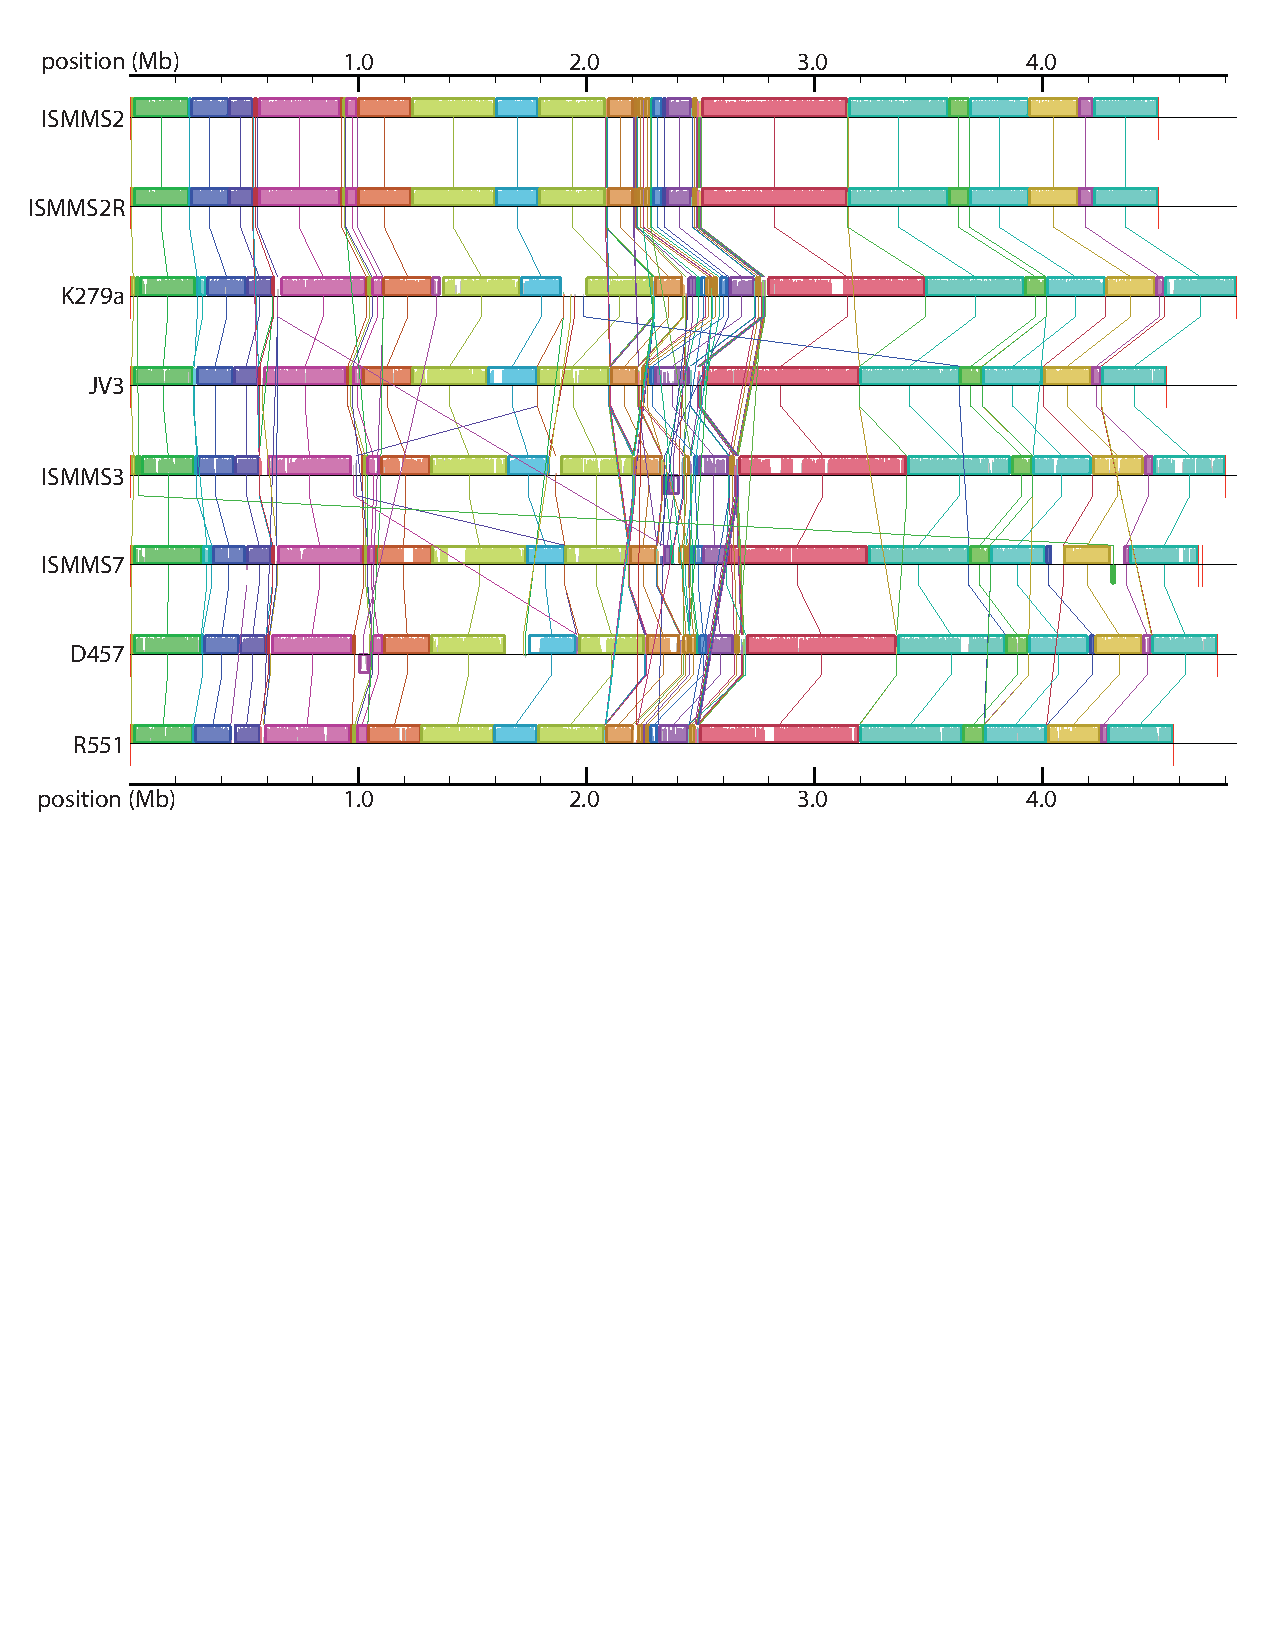
\includegraphics[width=\textwidth]{chap2/mauve_structural_variation}               
  \caption[Genome-scale comparison of four clinical isolates and four reference assemblies]{Genome-scale comparison of four fully assembled \emph{S. maltophilia} clinical isolates and four reference assemblies obtained from GenBank. Mauve 2.4.0 was used to plot locally collinear blocks (LCBs; conserved segments that appear to be internally free from genome rearrangements) as colored rectangles, with gaps representing non-homologous regions. Vertical bars inside each LCB rectangle show the average level of conservation at that region of the genomic sequence. Colored lines connect homologous LCBs among the genomes, and LCBs plotted below the centerline are in the reverse complement orientation relative to the ISMMS2 sequence. At top, sequences for the isolates from before and after development of quinolone resistance (ISSMS2 and ISSMS2R) in the case patient have identical structures.}
  \label{fig:mauve}
\end{figure}

Recombination is not an obvious source of diversity in our \emph{S. maltophilia} isolates. Figure \ref{fig:mauve} depicts whole genome alignments between the four clinical isolates where assembly produced a circularized chromosome and the four GenBank references, showing small areas of non-homology separating large regions of significant homology occurring generally in the same order for each genome. ISMMS2 and ISMMS2R are structurally identical, as expected for serial isolates, while recombination events among other strains are limited to small 1-2kb segments. Epigenetics motif analysis also suggests that the isolates are not related. Table \ref{tab:steno_epimotifs} shows different motifs in isolates from separate patients, implicating differences in type II \& III restriction modification systems between the isolates more likely to be caused by inter-strain/species horizontal transfer of methyltransferases than by intra-strain mutations.\autocite{Srikhanta2010} Together, this demonstrates that transmission did not occur among these six cases and that whole-genome sequencing can comprehensively capture genetic distances and structural variants among diverse clinical isolates of \emph{S. maltophilia}.

\begin{table}[ht]
  \centering
  \begin{tabular}{l l}
    \toprule
    Isolate name & Epigenetic motifs \\
    \midrule
    ISMMS2   & AGT\underline{A}CT \\
    ISMMS2R  & AGT\underline{A}CT \\
    ISMMS3   & None \\
    ISMMS4   & CAG\underline{A}G \\
    ISMMS5   & CTGG\underline{A}C, CACAN\underline{A}G \\
    ISMMS6   & CAAC\underline{A}C, CTG\underline{A}TG, CAACG\underline{A}C \\
    ISMMS7   & CAG\underline{A}G \\
    \bottomrule
  \end{tabular}
  \caption[Epigenetic motifs for clinical isolates of S. maltophilia]{Diverse epigenetic motifs, representing putative target sequences for each strain’s DNA methyltransferase enzymes, discovered for clinical isolates of \emph{S. maltophilia}.  Isolates are named as in Table \ref{tab:steno_pts}. The underlined A’s correspond to putative 6-methyladenine residues, which was the only modification type found in this study.}
  \label{tab:steno_epimotifs}
\end{table}

\section{Discussion}

This is the first report of WGS on serial isolates to characterize the emergence of a resistance mutation in \emph{S. maltophilia} during antibiotic treatment of an active infection. In contrast to studies sequencing highly resistant strains of \emph{S. maltophilia} to reveal various intrinsic and acquired antibiotic resistance genes,\autocite{Crossman2008,Zhao2015} where it remains difficult to assess their relative importance to the phenotype, performing WGS on serial isolates as resistance emerges in vivo allows the causative mutation(s) to be captured. In our patient, the mutation was a SNV that replicates a variant observed in an in vitro model strain created to study the MDR phenotype in 1997.\autocite{Alonso1997} Using WGS and susceptibility testing, we can confirm that this SNV was the only variant to emerge and that it was sufficient to confer quinolone resistance in a clinical case. This underscores the need for clinicians to consider repeating DST during monotherapy if clinical signs suggest therapy failure.

\emph{smeT} appears to play a central role in adaptive resistance to quinolones and other antibiotics effluxed by \emph{smeDEF}, like tetracycline, chloramphenicol, erythromycin, and aminoglycosides. Since any mutation that inactivates this protein would be able to derepress \emph{smeDEF} and confer resistance, \emph{smeT} is under intense selective pressure in the presence of these drugs. In this study, we observed not only a deleterious SNV in the strain that displayed resistance (ISMMS2R), but a premature stop codon in \emph{smeT} in a strain that was already resistant at first isolation (ISMMS4). Certain nucleotide positions appear to be under greater selective pressure than others, as evidenced by our observation of the same mutation that occurred in D457R, and a relative paucity of nonsynonymous coding mutations in \emph{smeT} observed among clinical \emph{smeT} isolates.\autocite{Sanchez2004} Since sustained overexpression of \emph{smeDEF} is physiologically unfavorable \autocite{Alonso2004}, it is possible that pathogenic strains of \emph{S. maltophilia} rely on natural diversity of mutations in the \emph{smeT} locus to activate or deactivate \emph{smeDEF} expression, allowing for rapid adaptation to antibiotic stress, though further study is needed.

Since resistance from a single SNV emerged during a short course of ciprofloxacin, clinicians should be cautioned about using quinolone monotherapy for \emph{S. maltophilia} bacteremia, as highlighted in recent retrospective studies.\autocite{Cho2014a,Wang2014} The wide variety of MDR phenotypes and unreliability of DST results has created uncertainty about appropriate treatment for \emph{S. maltophilia}, but SXT remains the most common choice for monotherapy.\autocite{Brooke2012,Cho2014a,Wang2014} SXT resistance in \emph{S. maltophilia} is not known to be caused by efflux systems but has been linked to Class 1 integrons and ISCR elements.\autocite{Brooke2012} This suggests that spontaneous resistance is less likely to emerge with SXT monotherapy, although a clinical trial comparing the two antibiotics is warranted.\autocite{Cho2014a,Wang2014}

In conclusion, characterizing the full extent of genetic alterations that \emph{S. maltophilia} utilizes to develop antibiotic resistance in vivo and improving genomic surveillance of clinical strains will help refine antibiotic selection criteria available to clinicians. This study furthermore highlights the utility of WGS for profiling the precise mutations underlying emerging antibiotic resistance in clinical cases of bacteremia.

\section*{Notes}

A shortened version of this chapter was published in \textit{Antimicrobial Agents and Chemotherapy}.\autocite{Pak2015a}

\subsection{Funding}

Funding was provided by the Icahn Institute for Genomics and Multiscale Biology at Mount Sinai, and also in part by the NIAID-supported NRSA Institutional Research Training Grant (5 T32 AI 7647-13) for Global Health Research (DRA).

\subsection{Conflict of Interest}

The authors have no conflicts of interest to disclose.

\subsection{Acknowledgements}

We thank Timothy O’Donnell, Tavi Nathanson, Jose Clemente, Flora Samaroo, Angelo Rendo, and members of the clinical microbiology laboratory at Mount Sinai for their contributions. This work was supported in part by the resources and expertise of the Department of Scientific Computing at the Icahn School of Medicine at Mount Sinai.
%% This is an example first chapter.  You should put chapter/appendix that you
%% write into a separate file, and add a line \include{yourfilename} to
%% main.tex, where `yourfilename.tex' is the name of the chapter/appendix file.
%% You can process specific files by typing their names in at the 
%% \files=
%% prompt when you run the file main.tex through LaTeX.

\chapter{Dummy chapter}

\begin{quote}
\textit{In this chapter, I describe my introduction. Lorem ipsum dolor sit amet, consectetur adipiscing elit. Aenean quis dolor bibendum, lobortis mauris a, sollicitudin lacus.}
\end{quote}

\newthought{Lorem ipsum dolor sit amet}, consectetur adipiscing elit. Aenean quis dolor bibendum, lobortis mauris a, sollicitudin lacus. Vivamus sollicitudin orci sed convallis faucibus. Morbi tempor augue vel nunc mollis euismod. Fusce varius fermentum dui, vel ultrices massa fermentum a. \marginnote{Check it out, here's a margin note.}  Pellentesque ac ipsum et libero cursus posuere. Aliquam tincidunt sapien ut ultrices dignissim. Cras tortor leo, pulvinar sagittis lacus et, convallis consectetur quam. Suspendisse potenti. Etiam convallis velit felis, eu rutrum ligula dictum sit amet.

Sed nec suscipit ex. Ut quis urna interdum tortor sollicitudin iaculis. Aliquam purus est, venenatis ac blandit quis, semper quis felis. Integer arcu augue, accumsan at vulputate sed, tristique eu libero.\autocite{Aghaeepour2013} Vivamus ut scelerisque massa. Pellentesque commodo arcu mollis dolor venenatis eleifend. Nulla sit amet rutrum nulla. Nullam leo ante, dapibus vel ipsum quis, bibendum condimentum ligula. Sed faucibus fermentum condimentum. Morbi eu ligula id lacus mattis pharetra. Phasellus auctor est sit amet sapien facilisis molestie vel in ipsum. Etiam malesuada vitae eros sed lacinia.\autocite{Rolph2015} Suspendisse eget iaculis odio, a molestie ex. Mauris ultrices et dolor nec dictum.\autocite{Rolph2015}

Vivamus elementum vehicula orci id mollis.\autocite{Aghaeepour2013,Gelman2006} Duis auctor sapien vel pretium bibendum. Nam aliquam, felis at efficitur pretium, justo libero cursus nisi, sit amet molestie metus massa nec sapien. Donec efficitur porttitor arcu et tempus. Phasellus pretium, diam id suscipit ultrices, lectus odio suscipit risus, at fermentum leo massa vitae eros. Donec elit orci, faucibus et aliquet quis, interdum eget lorem. Nulla a tincidunt odio, vitae commodo metus. Pellentesque bibendum cursus.\autocite{Rolph2015}

\section{Methods}

Aliquam purus est, venenatis ac blandit quis, semper quis felis. Integer arcu augue, accumsan at vulputate sed, tristique eu libero. Vivamus ut scelerisque massa. Pellentesque commodo arcu mollis dolor venenatis eleifend. Nulla sit amet rutrum nulla. Nullam leo ante, dapibus vel ipsum quis, bibendum condimentum ligula. Sed faucibus fermentum condimentum. Morbi eu ligula id lacus mattis pharetra. Phasellus auctor est sit amet sapien facilisis molestie vel in ipsum. Etiam malesuada vitae eros sed lacinia. Suspendisse eget iaculis odio, a molestie ex. Mauris ultrices et dolor nec dictum.

\begin{figure}[htb]
 	\includegraphics[width=\textwidth]{chap1/spin}               
 	 \caption{Check it out, it's a Spin \url{http://spin.media.mit.edu}}
  	\label{fig:spin}
\end{figure}

Phasellus eu nunc eget ante hendrerit porta. Etiam dignissim, mauris vitae luctus sollicitudin, metus purus iaculis tortor, eu lobortis arcu neque vitae ante. Donec egestas nec sem id vulputate. Ut efficitur non massa eget tempor. Nullam rhoncus odio sed dui fringilla semper. Nullam luctus odio felis, ac rutrum mauris maximus sodales. Phasellus non gravida nulla. Aenean congue sapien vitae facilisis luctus. Cum sociis natoque penatibus et magnis dis parturient montes, nascetur ridiculus mus. In laoreet ultrices tellus sed tincidunt. Aenean tempus, dui vel fermentum laoreet, sapien sapien facilisis turpis, vel volutpat sapien libero at mi. Maecenas eleifend libero in enim finibus, eu hendrerit ipsum ornare. Nulla placerat massa eget sapien tincidunt, non venenatis libero accumsan. Nunc ex lectus, rutrum sed varius sed, consectetur vel nisl. Aliquam eu eros vel metus sodales fermentum. Sed quis ultrices nisl, vel semper nibh (Table \ref{tab:sample_table}).

\begin{table}[ht]
  \centering
  \begin{tabular}{l l l l l}
    \toprule
    Column A & Column B & Column C & Column D & Column E \\
    \midrule
    A & B & C & D & E \\
    1 & 2 & 3 & 4 & 5 \\
    10 & 20 & 30 & 40 & 50 \\
    \bottomrule
  \end{tabular}
  \caption{A meaningless table}
  \label{tab:sample_table}
\end{table}

Donec elit orci, faucibus et aliquet quis, interdum eget lorem. Nulla a tincidunt odio, vitae commodo metus.

\subsection{Jiggering the pokery}

\newthought{Sed nec suscipit ex.} Ut quis urna interdum tortor sollicitudin iaculis. Aliquam purus est, venenatis ac blandit quis, semper quis felis. Integer arcu augue, accumsan at vulputate sed, tristique eu libero. Vivamus ut scelerisque massa. Pellentesque commodo arcu mollis dolor venenatis eleifend. Nulla sit amet rutrum nulla. Nullam leo ante, dapibus vel ipsum quis, bibendum condimentum ligula. Sed faucibus fermentum condimentum. Morbi eu ligula id lacus mattis pharetra. Phasellus auctor est sit amet sapien facilisis molestie vel in ipsum. Etiam malesuada vitae eros sed lacinia. Suspendisse eget iaculis odio, a molestie ex. Mauris ultrices et dolor nec dictum.\autocite{Rolph2015,Couderc2015}

Duis auctor sapien vel pretium bibendum. Nam aliquam, felis at efficitur pretium, justo libero cursus nisi, sit amet molestie metus massa nec sapien. Donec efficitur porttitor arcu et tempus. Phasellus pretium, diam id suscipit ultrices, lectus odio suscipit risus, at fermentum leo massa vitae eros. Donec elit orci, faucibus et aliquet quis, interdum eget lorem. Nulla a tincidunt odio, vitae commodo metus. Pellentesque bibendum cursus (Figure \ref{fig:spin_margin}).

Ut quis urna interdum tortor sollicitudin iaculis. Aliquam purus est, venenatis ac blandit quis, semper quis felis. Integer arcu augue, accumsan at vulputate sed, tristique eu libero. Vivamus ut scelerisque massa. Pellentesque commodo arcu mollis dolor venenatis eleifend. Nulla sit amet rutrum nulla. Nullam leo ante, dapibus vel ipsum quis, bibendum condimentum ligula.

\begin{marginfigure}
 	\includegraphics[width=\textwidth]{chap1/spin}  
  \singlespacing             
 	 \caption{Check it out, it's a Spin margin figure \url{http://spin.media.mit.edu}}
  	\label{fig:spin_margin}
\end{marginfigure}

%% A chapter for my PhD dissertation
%% First author: Theodore Pak
%%
%% Must be included from main.tex.

\chapter{The PathogenDB software suite for genomic clinical microbiology \& epidemiology}
\label{chap:pathogendb}

\providecommand{\pathogendbpipeline}{Pa\-tho\-genDB-\allowbreak pipe\-line}
\providecommand{\pathogendbcomparison}{Pa\-tho\-genDB-\allowbreak com\-pa\-ri\-son}
\providecommand{\pathogendbviz}{Pa\-tho\-genDB-\allowbreak viz}

\sidequote{\emph{Jurassic Park}}{
  \speaker{John Hammond:} Dennis, our lives are in your hands and you have butterfingers?
  
  \speaker{Dennis Nedry:} \emph{[laughs]} I am totally unappreciated in my time. You can run this whole park from this room with minimal staff for up to three days. You think that kind of automation is easy? Or cheap? You know anybody who can network eight connection machines and debug two million lines of code for what I bid for this job?
}

\sidequote{\smallcaps{HAL}\oldstylenumbers{9000}, \emph{\oldstylenumbers{2001}: A Space Odyssey}}{
  Let me put it this way, Mr.\ Amor. The 9000 series is the most reliable computer ever made. No 9000 computer has ever made a mistake or distorted information. We are all, by any practical definition of the words, foolproof and incapable of error.
}

\begin{quote}
\emph{Next-generation sequencing (NGS) technologies have reduced the cost of acquiring genomic data from active infections in hospitals, with the potential to rapidly characterize patient-to-patient transmission with extreme precision. However, there is no integrated software for converting NGS data into species identifications, phylogenies, and drug susceptibilities, with particularly few options including \emph{de novo} assembly. A clinical application would ideally provide a unified pipeline that runs semi-automated analyses to inform infection prevention and control interventions. We developed a modular open-source software suite called PathogenDB that implements major functionalities needed for genomic clinical microbiology and pathogen surveillance. A central laboratory information management system runs on a standard open-source Linux/Apache/MySQL/PHP stack. A modular genomics workflow, \pathogendbpipeline, automates de novo assembly, circularization, gene annotation, quality control, and epigenetic motif prediction. A comparative genomics module, \pathogendbcomparison, performs semi-automated phylogenetic analysis. Finally, a visualization suite, \pathogendbviz, integrates phylogenies and epidemiological data into a ``live view'' of putative transmissions mapped to hospital locations. Thus far, \pathogendbpipeline{} has been used to assemble and annotate 593 genomes from 7 species, and runs in <12 hours end-to-end. At The Mount Sinai Hospital, \pathogendbcomparison{} has genomically characterized one MRSA outbreak, two transmissions via solid organ transplant, and pseudo-outbreaks of \emph{S. maltophilia} and \emph{B. cepacia}. All three software packages are freely available on GitHub.
}
\end{quote}

\newthought{There is} increasing consensus that next-generation sequencing (NGS) technologies will eventually become mainstream equipment in clinical microbiology laboratories,\sidecite[-3cm]{Didelot2012,Harris2013,Joensen2014} considering that its nominal reagent cost is already within range of routine tests (\$25 per isolate for certain short-read technologies) and that it is likely to improve turnaround time and sample throughput for epidemiological investigations and hard-to-culture organisms.\autocite{Didelot2012,Koser2012} One significant barrier to this, as noted in Chapter \ref{chap:intro}, is that informatics and software infrastructure for the new diagnostic workflows afforded by these technologies are not yet widely available. While robotic culturing systems like Vitek and BD Phoenix include mature software packages for automating the executing and interpretation of routine tests, even integrating directly with standard laboratory information management systems (LIMS) so that results can be associated with patient metadata and sent directly back to ordering physicians via the electronic medical record (EMR), no such framework exists for genomic clinical microbiology.

We have already noted in Tables \ref{tab:id_bioinf_dbs} and \ref{tab:id_bioinf_tools} and in Chapter \ref{chap:intro} that many open source software packages exist for \emph{individual components} of such a pipeline but no end-to-end solution has yet been assembled by the research community. The most mature components that are currently available are typically steps closest to the sequencer, since the relatively small number of sequencing platforms and ubiquitous demand for certain invariant processing steps for their direct outputs (e.g., debarcoding and demultiplexing, filtering reads, quality control, alignment to a reference) have spurred researchers to create consensus solutions for them. Less mature are the steps involved in \emph{de novo} assembly and beyond this frontier, since the capability to finish assemblies without human intervention has only recently emerged\autocite{Bashir2012} and the underlying algorithms and heuristics are still an area of active research.\autocite{Sohn2016} Finishing, annotating, and comparing brand new bacterial assemblies, therefore, has been sufficiently niche that a standard distributable ``toolkit'' was not needed. However, as long-read sequencing continues to drop in price and complexity\footnote{The MinION, by Oxford Nanopore Technologies, is available in \$1,000 starter kits, plugs into a USB port, and produces reads up to 10kbp; see \textcite{Check2014}} and \emph{de novo} assembly for these platforms becomes more accessible, demand for pathways bringing these data into medical microbiology is bound to rise.\autocite{Judge2016}

Fortunately, the construction of new pipelines built around existing smaller tools is a typical task in bioinformatics—so common, in fact, that meta-tools are available for this very purpose.\autocite{Koster2012,Goecks2010,Jamil2013} The fact that a standard pipeline has been slow to emerge should not be considered a bad omen; in fact, this same situation existed for human genomes when short-read NGS technologies first emerged. As large-scale community resource projects like 1000 Genomes were launched to take advantage of NGS, efforts to develop standardized pipelines to execute those projects naturally followed and bore fruit. The landmark publication for 1000 Genomes was filed in 2010,\autocite{Durbin2010} and within the few short years that followed, the tools that were developed to enable the project's goals were released,\autocite{McKenna2010} refined into best practices for the community,\autocite{VanderAuwera2013} and reached sufficient maturity that they could be validated and adopted for use in clinical whole genome and whole exome sequencing pipelines.\autocite{Linderman2014} These tools, particularly Broad's Genome Analysis Toolkit (GATK), took what had previously been a hodgepodge of nascent data formats and algorithms and unified them into a consistently designed library with a uniform API. Furthermore, they were optimized for re-use in diverse and parallelized computing environments, and most importantly underwent battle-testing in enough real-world use cases to become de-facto standards. Given the rapid pace at which this occurred, we remain optimistic that similar widescale efforts in genomic microbiology can drive demand and community support for a similar toolkit for pathogens, and that such software's adoption can reach clinical laboratories within years of its initial release.\autocite{Pak2015}

Of course, there are many challenges that can be expected, although they generally fall into the category of engineering problems and can therefore leverage many of the lessons and algorithms already unearthed by human genomicists. The premise of a genomic microbiology pipeline gaining clinical use requires it to be fast, if not faster than substitutable lab tests like culturing.\autocite{Koser2012} Since this implies a turnaround time of one or two days, the software must be efficient. Ideally, it would not require the supercomputing power typically associated with human genomics, and could instead run on a single server or a desktop machine that any microbiology lab could afford.\footnote{Alternatively, labs could ``rent'' supercomputing power from cloud platforms like Amazon's Elastic Compute Cloud, but this introduces special complexities of its own.} Thankfully, bacterial genomic data are generally much smaller than their human counterparts, and many of the components in Table \ref{tab:id_bioinf_tools} were already developed for use on everyday desktop hardware. The software must be generally reliable, but seeing as no bioinformatics pipeline succeeds in real-world usage 100\% of the time (imagine contaminated DNA entering an analysis, or the computer running out of disk space), if it must fail, it should fail obviously and provide some clues as to where and why. If possible, it should save work up to the failed step so when analysis needs to be re-run, time does is not wasted re-running steps that previously succeeded. Perhaps most importantly, all steps need to be reproducible, because it would be extremely difficult (if not untenable on its face) to achieve diagnostic validity with a nondeterministic and therefore unauditable procedure. While this seems simple in principle for a computer program, in practice, with constantly changing sources of ``truth'' (such as changes in local and remote databases, updates to ancillary libraries, and evolving storage formats) it can be a devilishly complicated affair.

There are some recent examples of publicly released, self-contained pipe\-lines that use NGS to solve specific problems in clinical microbiology. One is SURPI, which processes millions of reads from a metagenomic sample to rapidly search for evidence of pathogen DNA.\autocite{Naccache2014} Most notably, this pipeline was used to deliver a timely diagnosis for a case of neuroleptospirosis that eluded traditional diagnostic assays.\autocite{Wilson2014} It can be deployed on both standalone servers and cloud computing environments.\autocite{Naccache2014} Another is Mykrobe, which similarly processes NGS reads to generate clinican-friendly reports of antimicrobial resistance predictions for \emph{Staphylococcus aureus} and \emph{Mycobacterium tuberculosis}, matching the results of gold-standard methods in 99\% of drug-strain combinations for the former and >80\% for the latter.\autocite{Bradley2015} Both of these are admirable for being self-contained packages that anybody can download and run (Mykrobe can even run on consumer-grade macOS and Windows laptops) and requiring only one input: raw NGS reads in the common FASTQ format. While third party comparisons have yet to be published, both claim to provide reliable and actionable data. Neither, however, performs epidemiological analysis, i.e., assessment of multiple samples for the likelihood of transmission.

Our goal was to create a software suite to support the aims of the Pathogen Surveillance Program at The Mount Sinai Hospital, which applies long-read and short-read NGS technologies to routinely collected clinical microbiology specimens and aims to track and prevent the spread of healthcare associated infections (HAIs) throughout our health system. As this is a much broader goal than attempted by the aforementioned software packages, we divided our design into four modular, coordinated components: a LIMS suitable for genomic clinical microbiology (PathogenDB), an all-purpose bacterial assembly and annotation pipeline for the PacBio RS II (\pathogendbpipeline), a comparative genomics toolkit for the outputs of that pipeline (\pathogendbcomparison), and finally a visualization platform to turn these data into something clinically actionable (\pathogendbviz). In this chapter, we present the implementation of each of these components, the results enabled by the entire software suite to date, and our plan to disseminate the tools for broader use.

\begin{sidewaysfigure}[hp]
  \sidewaysvspace
  \centering
  \includegraphics[width=\textwidth]{chap4/pipeline-diag}
  \fullwidthlabelcaption{fig:pipeline_diag}{Overview of the PathogenDB suite}{
  \textbf{Overview of the PathogenDB suite}. The three modular processing components, \pathogendbpipeline, \pathogendbcomparison, and \pathogendbviz, surround our custom LIMS, PathogenDB, which serves as the central ``source of truth.'' The design of these components (and the circular path of information) directly reflects the workflow proposed in Figure \ref{fig:emr_ngs_loop}—note that the direction of flow in this diagram is generally counter-clockwise while it is clockwise in Figure \ref{fig:emr_ngs_loop}.
  }
\end{sidewaysfigure}

\section{Implementation}

\newthought{A top-level view} of all steps and their relationships is presented in Figure \ref{fig:pipeline_diag}. We will review the details of each major component (boxed segments) in sequence. Note that our current design and separation of concerns directly reflects the large circular workflow of a ``learning health system'' for infectious diseases proposed earlier in Figure \ref{fig:emr_ngs_loop}.

\subsection{Sample collection}

The first step of any genomic surveillance project is to collect and organize samples, which is reflected in the workflow at the upper left of Figure \ref{fig:emr_ngs_loop}. This is performed by people, not software. In the case of the Pathogen Surveillance Program, the Bakel lab receives daily deliveries of specimens from Mount Sinai's clinical microbiology laboratory. Staff in this lab must carry out a meticulous process of labeling, culturing, stocking, subcloning, and extracting DNA before any sequencing can occur.

However, to track the specimens, stocks, and derivative samples and associate them with metadata created during patient care (top center of Figure \ref{fig:emr_ngs_loop}), a database is necessary. In our workflow, we call this database PathogenDB, and it serves as the critical central ``source of truth'' for all operations and analyses. PathogenDB receives updates via online input forms from the staff in the Bakel lab as they process samples. All items are barcoded and recorded in PathogenDB. The barcoding process, which involves assigning a new ID, both serves to unqiuely identify every item and to remove any pre-existing association with patient identifiers. Simultaneously, PathogenDB receives automatic nightly reports from the EMR (Epic Systems) which contain all the isolates that were expected to be sent for that day along with clinical metadata like the hospital unit of collection, the collection date and time, the bodily source of the specimen (blood, stool, wound, etc.), and an opaque patient ID that does not correspond to any patient IDs reflected in the actual medical record (like the medical record number). Only authorized staff, such as clinicians and infection prevention and control officers, are allowed to see the key linking patient metadata in PathogenDB to outside medical records. This is done to ensure de-identification of Protected Health Information in accordance with HIPAA Safe Harbor Method principles.\footnote{See \href{https://www.law.cornell.edu/cfr/text/45/164.514}{45 CFR §164.514(b)(2)}.}

PathogenDB is implemented as a MySQL database, and the relational structure for core tables is depicted in Figure \ref{fig:pdb_relations}. The structure of the database 
\begin{figure}[htb]
  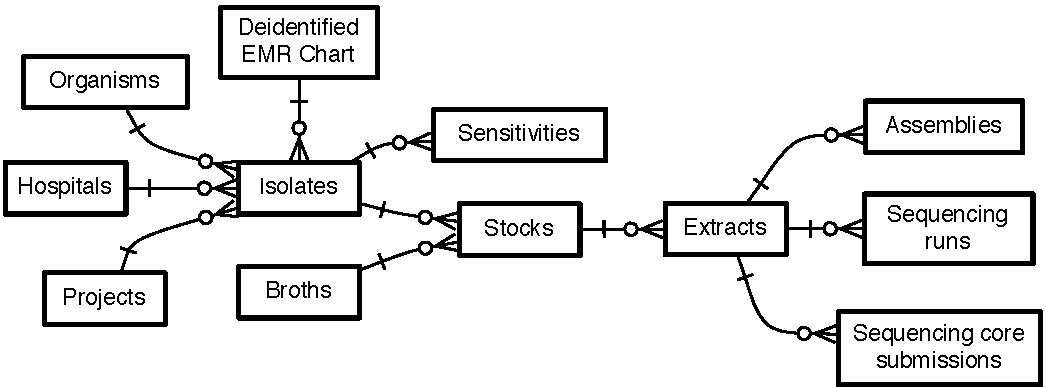
\includegraphics[width=\textwidth]{chap4/db-relations}               
  \caption[Entity-relationship diagram for the database underlying Pa\-tho\-gen\-DB]{\textbf{Entity-relationship diagram for the database underlying PathogenDB,} using Information Engineering notation; see \textcite{Halpin2010}. Boxes represent tables of entities; single lines represent relationships, with arrowheads indicating the cardinality of each side of the relationship; crow’s foot arrowhead with circle represents “zero or more;” cross-stroke arrowhead represents “exactly one.”}
  \label{fig:pdb_relations}
\end{figure}
mirrors the workflow of banking and preparing isolates, with steps proceeding roughly left to right starting from ``Isolates''—i.e., isolates can associated with one or more derivative stocks once culturing and banking are performed, which will then be associated with one or more extracts, which are then submitted to the Genomics Core Facilty at Mount Sinai (``sequencing core submissions''). The returned outputs from Genomics Core are logged as ``sequencing runs'' and then eventually ``assemblies'' are created upon completion of the \pathogendbpipeline{} (see next section). Maintaining database tables for each step of the process ensures that items are not lost along the way, and that the provenance of every downstream product can be traced backwards, which is crucial if contamination or mishandling are suspected.

\begin{sidewaysfigure}[hp]
  \sidewaysvspace
  \centering
  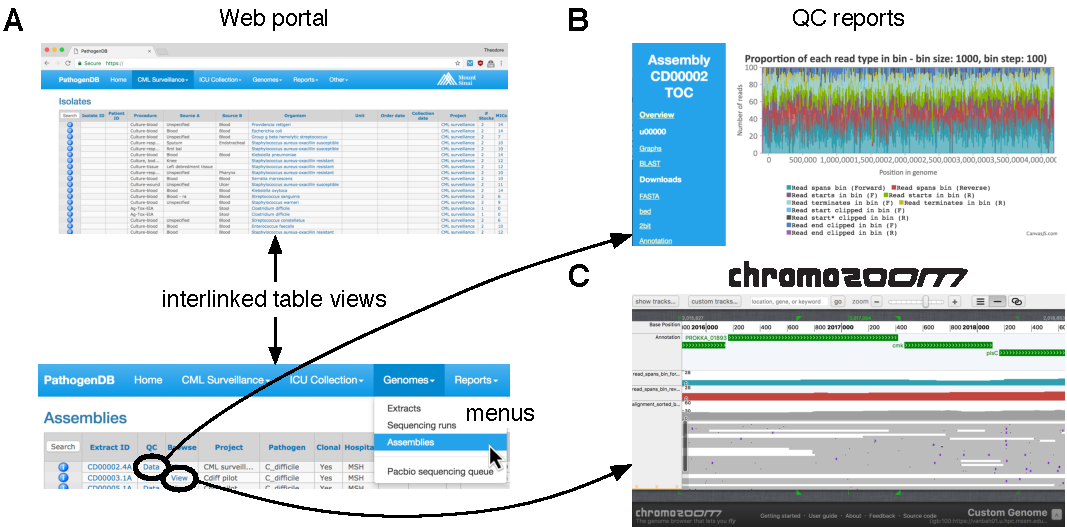
\includegraphics[width=\textwidth]{chap4/pdb-ui}               
  \fullwidthlabelcaption{fig:pdb_ui}{Overview of the web frontend for PathogenDB}{\textbf{Overview of the web frontend for PathogenDB.} A, the web portal permits quick access to basic views for all tables in the database, which can be searched, sorted, edited, and downloaded. At top, the Isolates table is shown, with certain potentially identifying information removed from the screenshot. At bottom, a zoomed view of the Assemblies table is shown, with the menu for switching between tables also shown. Links to special views (in B and C) are highlighted. B, sample quality control (QC) report for an assembly. Here, a graph of proportions of aligned reads that match various criteria is shown. Extreme fluctuations in these values can indicate assembly problems. C, ChromoZoom displaying a finished assembly, with annotated genes at top, two QC tracks in the center, and alignments of error corrected reads to the finished assembly at bottom. For more on ChromoZoom, see Chapter \ref{chap:chromozoom}.}
\end{sidewaysfigure}

PathogenDB provides a frontend that is based on phpMyEdit,\footnote{\url{http://www.phpmyedit.org/}} which is displayed in Figure \ref{fig:pdb_ui}. phpMyEdit allows for quick scaffolding of basic create-read-update-delete (CRUD) webpages for each of the tables in PathogenDB, which can be sorted, searched, edited, and downloaded by authorized members of the team. Authorization can be granted only to particular pages and views so that Bakel lab staff see only tables related to the isolate culturing and extraction workflow, while clinical coordinators instead see tables on patients due for sample collection and forms for sample submission.

Figure \ref{fig:pdb_ui}A shows a sample table view for the Isolates table, which tracks every biosample received by the Pathogen Surveillance Program. Isolates are associated with a Projects; if collected as part of routine operations, this is ``CML surveillance,'' but this field accommodates annotation of samples acquired from ad-hoc and outside investigations. Links at the far right of the table for Stocks and Minimum Inhibitory Concentrations (MICs) indicate that most Isolates are associated with two stocks and up to 14 measurements of antimicrobial susceptibility, which are extracted from Vitek (bioMérieux) results in the reports sent nightly by the EMR. Clicking on these links moves the user to a view of the corresponding entries in the related tables. On the Assemblies page, shown at the bottom of this panel, special views are provided for viewing outputs of the \pathogendbpipeline{} (after assembly and annotation are complete). The first of these is a quality control (QC) report (Figure \ref{fig:pdb_ui}B), which shows plots of the final contig layout and read statistics, which can be useful for assessing trustworthiness of the assembly and diagnosing reasons for failure to circularize or high fragmentation. The second of these is a link to a ChromoZoom visualization of the genome (Figure \ref{fig:pdb_ui}C, also see Chapter \ref{chap:chromozoom}).

\subsection{\pathogendbpipeline: Assembly and annotation from long reads}

Once read data are available from the Genomics Core, computational analysis can begin. To date, the Pathogen Surveillance Program has chosen to sequence essentially all isolates on the PacBio RS II (see Methods, Chapter \ref{chap:steno}). This sequencing platform comes with a manufacturer-maintained analysis toolkit called SMRT-Analysis\footnote[][-2.5cm]{\url{https://github.com/PacificBiosciences/SMRT-Analysis}} that we leverage for certain steps, which even includes a web interface (SMRT Portal), but we focus here on a fully automated solution.

\begin{figure*}[hb]
  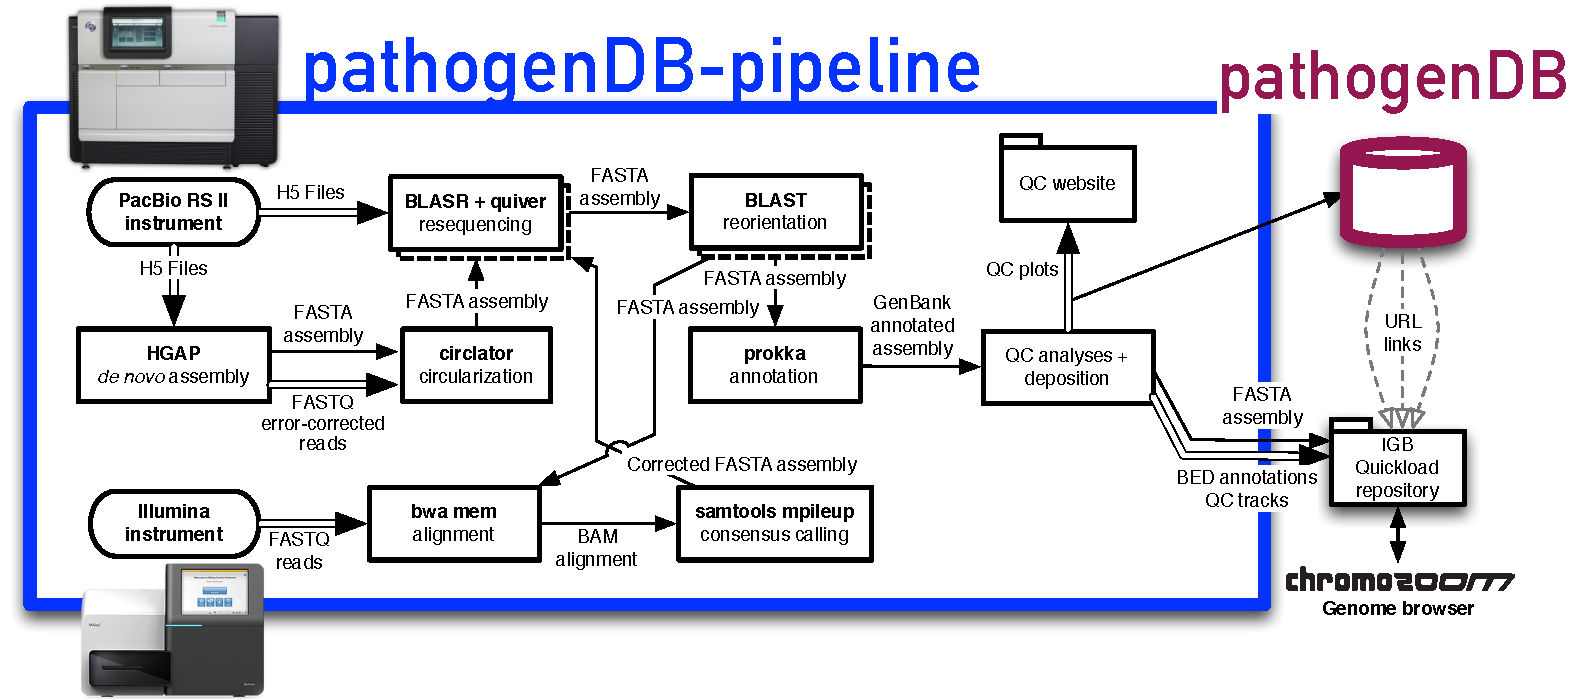
\includegraphics[width=\textwidth]{chap4/pdb-pipeline}               
  \caption[Outline of steps automated by \pathogendbpipeline]{\textbf{Outline of steps automated by \pathogendbpipeline.} Processes are depicted as boxes, with processes requiring potentially multiple runs indicated as a ``stack.'' An interim file format is depicted as a single arrow, and groups of files as doubled arrows. The pipeline concludes with deposition of a link to an IGB Quickload Directory for the completed assembly into PathogenDB.}
  \label{fig:pdb_pipeline}
  \setfloatalignment{b}
\end{figure*}

The chosen strategy for converting PacBio RS II reads into a final annotated assembly is outlined in Figure \ref{fig:pdb_pipeline}. Briefly, the H5 outputs of the instrument (which contains movies of the single molecule reads) are assembled \emph{de novo} using the Hierarchical Genome Assembly Process\autocite{Chin2013} (HGAP), which is included in SMRT-Analysis. This produces a draft assembly, but since HGAP cannot create circular contigs, a FASTA of this assembly and the FASTQs of error-corrected reads produced by HGAP are passed off to \texttt{circlator},\autocite{Hunt2015} a recently released tool that automates \emph{circularization} by using SPAdes\autocite{Bankevich2012} to re-assemble the error-corrected reads that overlapped the ends of contigs. This produces a new assembly that is then \emph{polished} over the circularized junctions by re-mapping raw reads using BLASR\autocite{Chaisson2012} and recalling the consensus with Quiver,\autocite{Chin2013} which reduces errors in these regions by re-incorporating read information that could not have aligned properly during the initial HGAP assembly. The polished assembly is then \emph{reoriented} back to the origin of replication (a convention for GenBank bacterial chromosome sequences) using a custom script\footnote{ \texttt{scripts/post\textunderscore quiver\textunderscore orient\textunderscore correct.py} in the \href{https://github.com/powerpak/pathogendb-pipeline/blob/master/scripts/post\textunderscore quiver\textunderscore orient\textunderscore correct.py}{GitHub repo}.} that performs a BLAST against \texttt{circlator}'s suggested origin point for each circular contig, which it decides based on a PROmer\autocite{Kurtz2004} search for \emph{dnaA} sequences.

The circularized, polished, and reoriented assembly is finally ready for annotation. Firstly, the contigs are renamed from the overly verbose HGAP and Quiver defaults. We use an in-house convention of starting all contig names with ``\texttt{u}'' (for ``unitig'', a term from Celera\footnote{See \url{http://wgs-assembler.sourceforge.net/wiki/index.php/Celera_Assembler_Terminology}}) followed by a five-digit unitig number originally assigned by HGAP. This is followed by three letters that flag for \underline{c}ircularization, \underline{r}eorientation, \underline{p}olishing, and an additional letter reserved for later use, with ``\texttt{x}'' indicating failure of that step. Another letter surrounded by underscores signals the hypothesized type of contig (\underline{c}hromosome, \underline{p}lasmid, \underline{m}erged, \underline{g}arbage, or \underline{o}ther).\footnote{We use the simple heuristic that any successfully circularized contig >1Mbp is a chromosome, and anything smaller is a plasmid. Merged and garbage contigs are the result of ambiguities during assembly. For more detail, see \href{https://github.com/powerpak/pathogendb-pipeline/blob/master/scripts/post\textunderscore circlator\textunderscore contig\textunderscore rename.py}{\texttt{scripts/post\textunderscore circlator\textunderscore contig\textunderscore rename.py}}.} Finally, the original SMRT-analysis job number set by the Genomics Core is appended. This renaming results in a contig ID like \verb|u00011crpx_p_023011|, indicating it is the 11th unitig, was \underline{c}ircularized, \underline{r}eoriented, and \underline{p}olished, is probably a \underline{p}lasmid, and came from sequencing job \#023011. These names are short enough for easy viewing in downstream tools like ChromoZoom, while retaining as much information as possible about the provenance and assembly status of the contig. Renamed contigs are finally annotated with \texttt{prokka},\autocite{Seemann2014} which detects putative coding regions and maps them to annotated gene names in UniProt.\autocite{Wasmuth2016} We then run a series of custom scripts to generate diagnostic files for the QC webpage (Figure \ref{fig:pdb_ui}B) and to convert the assembly and related tracks into an IGB Quickload Directory that can be loaded into ChromoZoom (Figure \ref{fig:pdb_ui}C).

\newthought{\pathogendbpipeline{}} is implemented as a \texttt{Rakefile}, which is written in Ruby and executed by \texttt{rake}, an analog of GNU \texttt{make}.\footnote{GNU \texttt{make} also inspired SnakeMake, a bioinformatics-focused build system for Python; see \textcite{Koster2012}.} GNU \texttt{make} was originally written as a build system for automating the generation of executables and other products from a program's source files. The advantage of a build system is that it encourages the explicit annotation of dependencies between interim files and tasks into the pipeline, thereby allowing for previous products of a partial build to be automatically re-used if their dependencies (source files) have not changed. From the user's perspective, another benefit is that only the desired final task in the pipeline needs to be specified, and \texttt{rake} can automatically figure out what preceding tasks are required to get to that point. For most runs, the sequence of tasks selected by \pathogendbpipeline{} is the following:

\begin{enumerate}[label=\arabic*.,noitemsep,labelindent=2em,leftmargin=!]
\item \verb|pull_down_raw_reads|
\item \verb|assemble_raw_reads|
\item \verb|run_circlator|
\item \verb|post_circlator|
\item \verb|resequence_assembly|
\item \verb|post_quiver_orient_correct|
\item \verb|prokka_annotate|
\item \verb|create_QC_webpage|
\item \verb|prokka_to_igb|
\end{enumerate}

which mostly correspond, unsurprisingly, to the boxes in Figure \ref{fig:pdb_pipeline}. Most of these tasks require at least one configuration option, such as the expected species or the destination for output. These are specified as environment variables during invocation, so to get to the final \verb|prokka_to_igb| step above, the user would run something like:

\begin{verbatim}
    $ rake OUT=scratch/out/ER05681 \
           SMRT_JOB_ID=023154 \
           STRAIN_NAME=ER05681 \
           SPECIES="Staphylococcus aureus" \
           prokka_to_igb
\end{verbatim}

If problems occur during assembly, the pipeline supports manual editing of the interim FASTA files, and then a flag (\texttt{CURATED=1}) can be set to signify that manual curation occurred and to therefore bypass circularization, reorientation, and contig renaming. There is also an optional branch (bottom entry point for Figure \ref{fig:pdb_pipeline}) that can incorporate Illumina short reads during assembly. Auxiliary sequencing on a short read platform can correct small errors that HGAP on PacBio reads will miss—typically indels in homopolymeric stretches. For this branch, \texttt{bwa}\autocite{Li2010b} is used to perform in-memory alignment against the circularized, reoriented, and polished assembly, and \texttt{samtools}\autocite{Li2009b} and \texttt{vcftools}\autocite{Danecek2011} are used to call variants from the pileup and create a new FASTA consensus. These steps can in fact be repeated several times (crossover loop in Figure \ref{fig:pdb_pipeline}) to call a progressively more accurate consensus, although this repetition must currently be invoked manually.\footnote{A future version of the pipeline might attempt to re-run the steps until the consensus stabilizes.}

The modularity of siloing tasks in a \texttt{Rakefile} provided long-term advantages besides those mentioned previously. In our case, when we first created the pipeline in 2013, mature tools for some of the steps did not yet exist, e.g., \texttt{circlator} and \texttt{prokka} were not yet publicly available. Therefore, we used less efficient solutions, such as our own custom script for circularization and the RAST web service\autocite{Aziz2008} for annotation, as in Chapter \ref{chap:steno}. Once mature tools became available, it was relatively simple to swap them into the pipeline while preserving the old code under an \texttt{old:} namespace, indicating tasks that are deprecated. Because each task and its dependencies are relatively isolated, different members of the team can create slightly different versions of certain interim steps while still sharing all code in one common \texttt{Rakefile} pipeline. This was of course further reinforced by keeping all code under version control.\footnote{\url{https://github.com/powerpak/pathogendb-pipeline}}

\subsection{\pathogendbcomparison: Rapid comparative genomics}

\newthought{After deposition} of a complete annotated assembly's IGB Quickload Directory and corresponding record into the Assemblies table of PathogenDB, the next logical step of analysis is to compare all genomes for a given species (perhaps with some filtering by timeframe or location) to determine relatedness and the likelihood of transmissions. We implemented these analyses within the next module of our suite, called \pathogendbcomparison.

\begin{figure*}[htb]
  \centering
  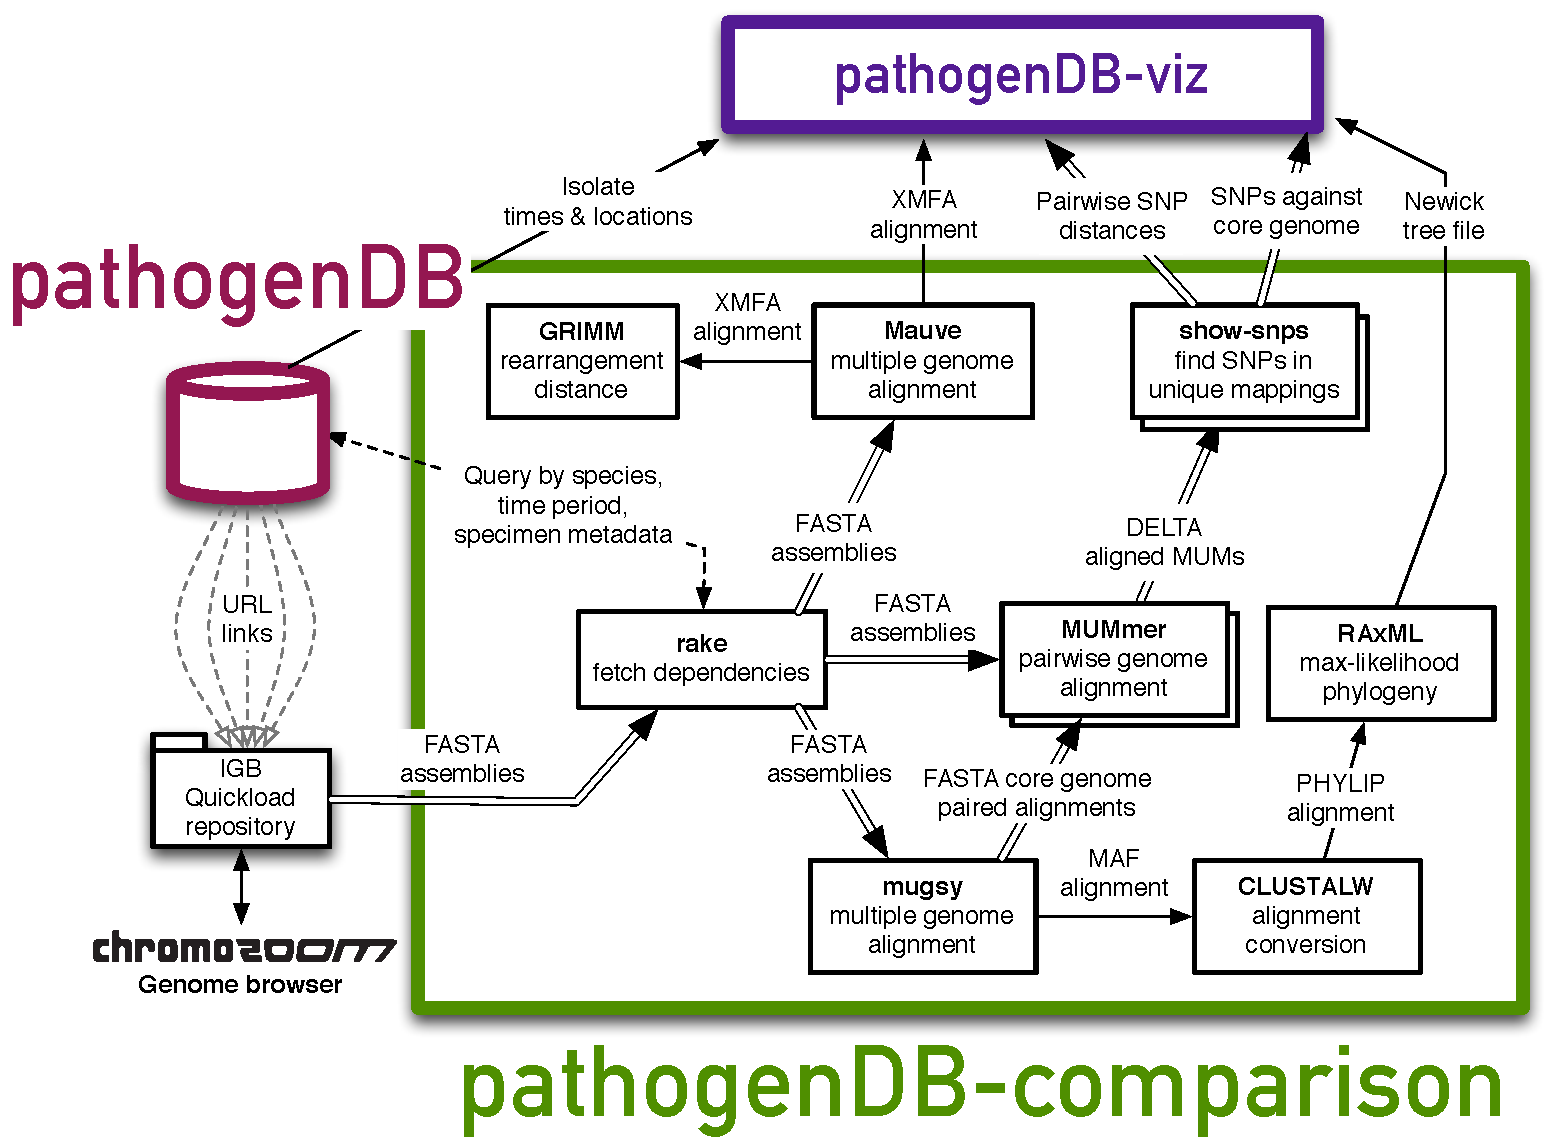
\includegraphics[width=0.8\textwidth]{chap4/pdb-comparison}               
  \caption[Outline of steps automated by \pathogendbcomparison]{\textbf{Outline of steps automated by \pathogendbcomparison.} Processes are depicted as boxes, with processes requiring potentially multiple runs indicated as a ``stack.'' An interim file format is depicted as a single arrow, and groups of files as doubled arrows. The pipeline concludes with various outputs being sent to \pathogendbviz{} for further visualization.}
  \label{fig:pdb_comparison}
\end{figure*}

Our implementation of workflows for this stage of analysis is outlined in Figure \ref{fig:pdb_comparison}. As emphasized previously, PathogenDB is considered the single source of ``truth'' from which all assemblies and metadata are queried before running an analysis; however, some of the tasks are generic enough to run on an arbitrary set of FASTA files without metadata. Like \pathogendbpipeline, \pathogendbcomparison{} is also implemented using \texttt{rake}, but its workflow is more branched. The three types of implemented analyses, reflected in Figure \ref{fig:pdb_comparison} by the three arrows emerging from the \texttt{rake} box and listed here with their corresponding \texttt{rake} task names, are:

\begin{enumerate}[label=\arabic*.,noitemsep,labelindent=2em,leftmargin=!]
\item \verb|mauve|: Mauve alignment, which highlights structural variants
\item \verb|snv|: Pairwise MUMmer single nucleotide variant (SNV) distances for heatmap visualization
\item \verb|mugsy|: Core genome alignment for a phylogeny with branch lengths scaled to SNV distances
\end{enumerate}

A Mauve alignment of \emph{S. maltophila} genomes was previously depicted in Figure \ref{fig:mauve} and is most useful for finding large insertions, deletions, translocations, and other recombinatorial events. Mauve performs alignments by using an anchoring heuristic to search for large areas of homology among subsets of the input genomes, which it terms local collinearity blocks (LCBs).\autocite{Darling2010} Our corresponding task simply wraps execution of \texttt{progressiveMauve}\autocite{Darling2010} and returns the XMFA alignment, since visualization is typically performed with the Mauve Java application. However, we also provide a task that can calculate pairwise rearrangement distances using GRIMM,\autocite{Tesler2002} which searches for the minimal number of inversion operations needed to transform one genome's sequence of LCBs into another genome's. Because inversion distance is algorithmically simple to calculate\autocite{Hannenhalli1999} but probably reflects evolutionary edit distances less accurately than newer models like double-cut and join (DCJ),\autocite{Lin2008} we have not yet made full use of these distances, but hope to eventually incorporate a wide array of structural variant edit distances into downstream analysis.\autocite{Hilker2012}

MUMmer is a versatile software suite for fast pairwise genome alignment that finds maximally exact matches (formerly maximal unique matches, hence MUM) using a suffix tree algorithm that can run in linear time.\autocite{Kurtz2004} Although it is excellent for finding subsequences of one genome that are within a certain edit distance of all locations on another genome, because of the strict edit distance threshold, it is less suited for finding large rearrangements compared to Mauve. However, it is very well suited for quickly calling SNVs between two genomes, as long as the SNVs are not so closely spaced as to elude a maximally exact match for the surrounding region (which should occur only extremely rarely). For this task, we use the \texttt{show-snps} tool within MUMmer to call SNVs between all pairs of input genomes, which produces a distance matrix that can be visualized with \pathogendbviz{} (see Results).

The same strategy is also used to rescale branches for our phylogenetic analysis, which we perform by creating a core genome alignment with \texttt{mugsy},\sidecite[-2cm]{Angiuoli2011a} a multiple genome aligner that internally combines MUMmer and its own algorithm for finding LCBs.\footnote[][-2cm]{Recently, the Harvest suite was released for core genome alignment, which scales better to thousands of genomes than \texttt{mugsy}, and it even includes its own visualization tool, \texttt{gingr}. We are currently in the process of incorporating these tools into our pipeline. For more, see \textcite{Treangen2014}} The core genome alignment in MAF format is converted to PHYLIP format with CLUSTALW,\autocite{Sievers2011} and then this alignment undergoes maximum-likelihood phylogenetic inference via RAxML.\autocite{Stamatakis2005} Since the outputted tree (in Newick format) initially has distances in units of time under the RAxML evolutionary model, which is more opaque than SNV distance, the tree's branches are rescaled by recalculating SNV distance using the aforementioned \texttt{show-snps} method on all adjoining nodes, including the ancestral states imputed by RAxML. Phylograms of these trees with overlaid SNV distances (as in Figure \ref{fig:steno_phylo}) can be plotted to PDFs using an included \verb|mugsy_plot| task that wraps the \texttt{ape} R package.

Although maximum likelihood phylogenetic analysis is a standard component of molecular epidemiology and typically the centerpiece of most published investigations of outbreaks using NGS,\autocite{Azarian2015,Eyre2012,Joensen2014,Casali2016} it may in fact be overkill for answering the simpler day-to-day question of ``are any new isolates closely related to the previously sequenced isolates?'' By design, it requires a core genome alignment for all of the genomes that one wishes to include in the tree. Although every multiple sequence aligner uses heuristics to save time, multiple sequence alignment has a fundamental algorithmic complexity of $O(g^n)$ under the usual dynamic programming approaches,\autocite{Just2004} where $g$ is the average length of a genome and $n$ is the number of genomes—i.e., exponential to the number of genomes. Even though tools for core genome alignment continue to get smarter and faster about subverting this complexity,\autocite{Treangen2014} given the fundamental difficulties in scaling that problem, we anticipate that pairwise distance matrices will be a suitable alternative for outbreak detection as databases of thousands of assembled sequences become commonplace. Creating a distance matrix is guaranteed to be $O(n^2)$ in the most naive approach,\footnote{And this is how it is currently implemented; precalculating the MLST for all isolates and only allowing within-MLST comparisons would be a simple first optimization.} with each pairwise comparison being $O(g)$ by use of \texttt{show-snps}. Furthermore, adding one new assembled isolate does not require recalculating everything as in multiple sequence alignment, but we can instead add one row and column to the existing matrix in $O(2n)$ time. For these reasons we provide the \verb|snv| task in conjunction with \verb|mugsy|, and we rely on the distance matrices for analyses on >100 genomes, as presented later in the Results.

\subsection{\pathogendbviz}

\newthought{Visualization} is finally performed with the \pathogendbviz{} toolkit. The interface, which has a heatmap layout and a geospatial layout, will be presented in the Results in Figures \ref{fig:pdb_heatmap_saureus}-\ref{fig:pdb_geospatial_cdiff}. \pathogendbviz{} reads data from JSON files containing genetic distances and isolate metadata as prepared by \pathogendbcomparison{}'s \verb|heatmap| task, and displays it in a HTML5 interface that draws data dynamically to scalable vector graphics (SVG) using the d3.js Javascript library.\footnote{\url{https://d3js.org/}} \pathogendbviz{} is currently implemented as a single PHP page that loads all data via Asynchronous Javascript and XML (AJAX).\autocite{Paulson2005} Given that all data is drawn on the client side, it attempts to maximize the control the user has over the selection of isolates to displayed and how the comparison is presented. Agglomerative hierarchical clustering is performed in the browser using the \texttt{ml-hclust}\footnote{\url{https://www.npmjs.com/package/ml-hclust}} node.js package, using single linkage to emphasize the ``chaining'' of closely related genomes into clusters. The heatmap.js\footnote{\url{https://www.patrick-wied.at/static/heatmapjs/}} library is used to draw density plots of epidemiological incidence in the geospatial layout. Sequenced isolates are displayed in the geospatial layout as a live-updating force-directed network using \texttt{d3.forceSimulation}, with a strong force keeping nodes from colliding, a moderate force pulling nodes toward the position of specimen collection, and a very weak spring force along the edges (which represent the putative transmissions under the selected SNV threshold).

\subsection{Availability}

Source code for \pathogendbpipeline, \pathogendbcomparison, and \pathogendbviz{} is publicly available from GitHub at:

\begin{enumerate}[label=\arabic*.,noitemsep,labelindent=2em,leftmargin=!]
\item \url{https://github.com/powerpak/pathogendb-pipeline}
\item \url{https://github.com/powerpak/pathogendb-comparison}
\item \url{https://github.com/powerpak/pathogendb-viz}
\end{enumerate}

The code in each repository is still under active development to suit the operational needs of the Pathogen Surveillance Program. The software is currently configured for execution on Mount Sinai's high performance computing environment (Minerva), but we will adapt it for simple installation on vanilla Linux distributions and provide machine images suitable for common cloud computing environments once we are ready to promote usage by other groups.

\section{Results and Discussion}

\subsection{Assembly quality}

As of April 2017, \pathogendbpipeline{} has been used to assemble and annotate 593 genomes from 7 species. General statistics on assemblies produced by the pipeline are presented in Table \ref{tab:pathogendb_assemblies}. Most of the isolates assembled so far are \emph{Staphylococcus aureus} and \emph{Clostridium difficile} strains. About three quarters of the assembled \emph{S. aureus} isolates were methicillin-resistant (MRSA). A few other rarer species have also been assembled.\footnote{Note that the \emph{S. maltophilia} isolates from Chapter \ref{chap:steno} predate PathogenDB and therefore are not included in Table \ref{tab:pathogendb_assemblies}.} 164 assemblies underwent manual curation during the development of the pipeline and are excluded from statistics on assembly quality.

\begin{table}[htb]
  \centering
\small
\begin{tabular}{l l}
  \toprule
  Characteristic &
  Assemblies (\%), \emph{N}=593\\
  \midrule
  Species
  \\
  \-\tabindent \emph{Clostridium difficile} &
  221 (37.3)
  \\
  \-\tabindent \emph{Staphylococcus aureus}
  \\
  \-\tabindent\tabindent Methicillin-resistant &
  262 (44.3)
  \\
  \-\tabindent\tabindent Methicillin-resistant &
  90 (15.2)
  \\
  \-\tabindent \emph{Clostridium innocuum} &
  4 (0.7)
  \\
  \-\tabindent \emph{Enterococcus faecium} &
  4 (0.7)
  \\
  \-\tabindent Other &
  7 (1.1)
  \\
  \\
  Assembly quality (uncurated assemblies only) &
  Assemblies (\%), \emph{N}=429
  \\
  \midrule
  \-\tabindent \emph{N50} > 1Mbp &
  412 (96.0)
  \\
  \-\tabindent Circular chromosome$^a$ &
  303 (70.6)
  \\
  \-\tabindent Largest contig size
  \\
  \-\tabindent\tabindent ≥1Mbp &
  418 (97.4)
  \\
  \-\tabindent\tabindent ≥100kbp, <1Mbp &
  8 (1.9)
  \\
  \-\tabindent\tabindent <100kbp &
  3 (0.7)
  \\
  \-\tabindent Number of contigs
  \\
  \-\tabindent\tabindent 1 &
  102 (23.8)
  \\
  \-\tabindent\tabindent 2 &
  110 (25.6)
  \\
  \-\tabindent\tabindent 3 &
  71 (16.6)
  \\
  \-\tabindent\tabindent 4 &
  40 (9.3)
  \\
  \-\tabindent\tabindent ≥5 &
  84 (19.6)
  \\
  \bottomrule
\end{tabular}
  \caption[Statistics on assemblies generated by \pathogendbpipeline{} since 2013]{\textbf{Statistics on assemblies generated by \pathogendbpipeline{} since 2013.} Abbreviations: \emph{N50}, shortest contig length above which 50\% of the genome is included; Mbp, 1 million base pairs; kbp, 1 thousand base pairs.
  \captionfootnotetext{a}{Any contig ≥1Mbp that circularized was considered a chromosome.}
}
  \label{tab:pathogendb_assemblies}
\end{table}

Without any curation (manual fixes), \pathogendbpipeline{} is able to completely assemble most of the sequenced isolates, with >70\% featuring a circular main chromosome. The \emph{N50}, defined as the shortest contig at which it and all larger contigs would include 50\% of the genome, was ≥1Mbp for 96.0\% of uncurated genomes. 80.4\% of completed assemblies contained four or fewer contigs, i.e., one chromosome (either closed or unclosed) and up to three plasmids or unassembled fragments. By these metrics, \pathogendbpipeline{} is clearly able to produce many high-quality \emph{de novo} assemblies without human intervention.

\subsection{Computational benchmarks for \pathogendbpipeline}

\begin{figure*}[htb]
  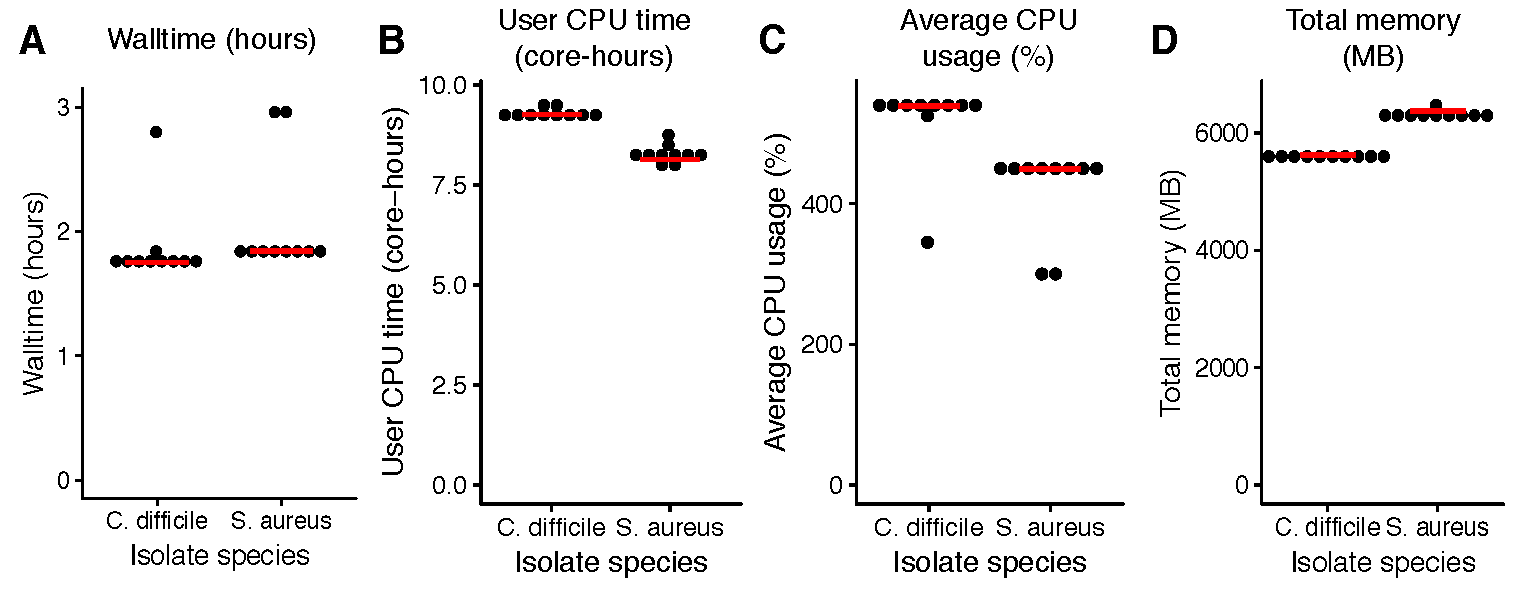
\includegraphics[width=\textwidth]{chap4/pdb-benchmark}               
  \caption[Dotplots of computational benchmarks for \pathogendbpipeline]{\textbf{Dotplots of computational benchmarks for \pathogendbpipeline{} on a \emph{S. aureus} and a \emph{C. difficile} isolate.} For each isolate, measurements were collected from 10 end-to-end serial runs of the pipeline, starting at raw read data and ending at the \texttt{prokka\textunderscore to\textunderscore igb} task, using a single server with a 12-core Intel Xeon® 2.5GHz E5-2680 CPU and 128GB of RAM. Horizontal red lines indicate the median.}
  \label{fig:pdb_benchmark}
\end{figure*}

Although over the past four years of development its end-to-end time has improved, \pathogendbpipeline{} is still by far the most computationally intensive module within the PathogenDB suite. The majority of the cost is accrued during the \emph{de novo} assembly and polishing steps, which require stepping through all read data for each sequenced isolate, which commonly exceeds 1Gbp per isolate. In Figure \ref{fig:pdb_benchmark} we provide benchmarks for the impact of \pathogendbpipeline{} on overall turnaround time for an end-to-end analysis and the corresponding computational cost. We performed 10 serial end-to-end runs of the pipeline starting from raw read data for one \emph{S. aureus} isolate and one \emph{C. difficile} isolate on a 12-core Intel Xeon® 2.5GHz E5-2680 server with 128GB of RAM. Most of the runs produced nearly identical benchmarks. The median walltime (which measures real-world start to end time) was under two hours, with none of the runs exceeding three hours (Figure \ref{fig:pdb_benchmark}A). The jobs benefited from multicore usage, as the median user CPU time in core-hours exceeded the walltime by a factor of 4-5× (Figure \ref{fig:pdb_benchmark}B), and this is confirmed by checking average CPU usage, which is normalized against a single core and stayed mostly in the 400-600\% range (Figure \ref{fig:pdb_benchmark}C). Although HGAP, BLASR, and Quiver are memory-intensive steps, the total memory used did not exceed 7GB for any of the runs (Figure \ref{fig:pdb_benchmark}D).

\subsection{\pathogendbviz{} characterizes local outbreaks of \emph{S. aureus}}

After comparing a large number of same-species isolates with \pathogendbcomparison{}, the analyses can be presented to clinicians in an interactive visualization using \pathogendbviz. Figure \ref{fig:pdb_heatmap_saureus} displays the interface of \pathogendbviz{} for a heatmap visualization of all \emph{S. aureus} isolates that clustered with at least one other patient's isolate(s) at a SNV threshold of ≤10 SNVs. The software provides a web interface with many controls for quickly ``drilling down'' to the time range and isolates of interest. We now briefly tour this interface.

\begin{sidewaysfigure}[hp]
  \sidewaysvspace
  \centering
  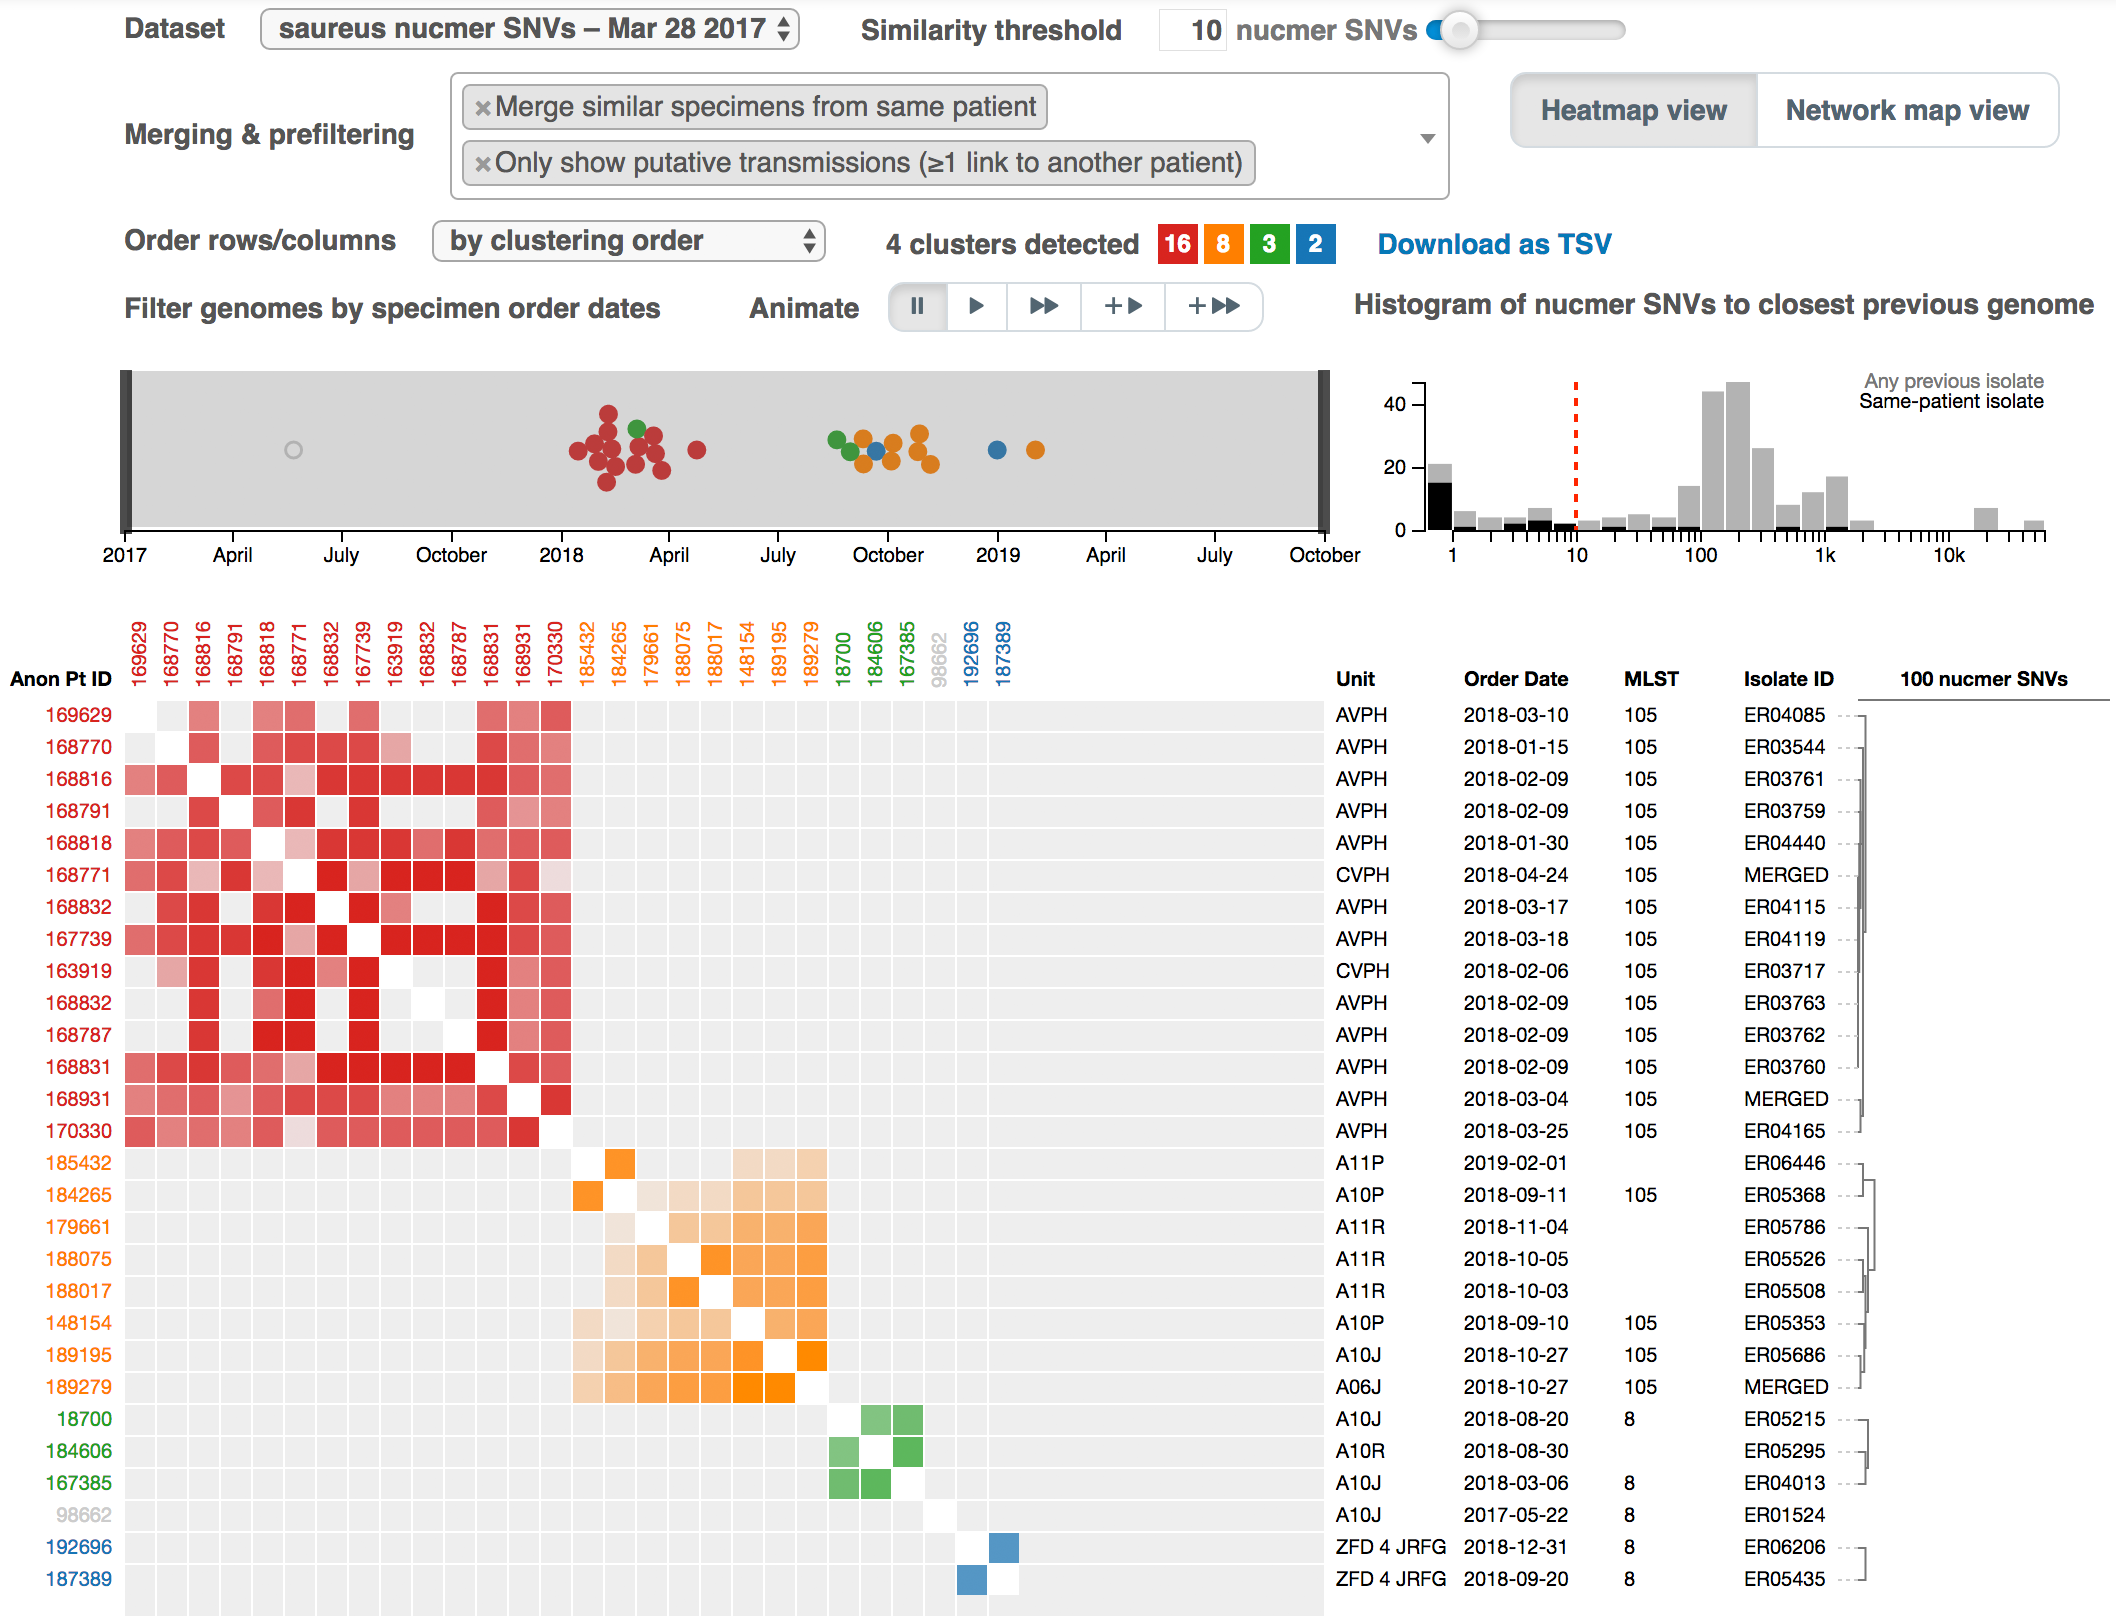
\includegraphics[width=0.85\textwidth]{chap4/pdb-heatmap-saureus}               
  \fullwidthlabelcaption{fig:pdb_heatmap_saureus}{\pathogendbviz{} heatmap visualization for all putatively transmitted \emph{S. aureus} isolates, based on NGS}{\textbf{\pathogendbviz{} heatmap visualization for all putatively transmitted \emph{S. aureus} isolates, based on NGS.} Note that dates have been shifted into the future and unit names have been obfuscated to reduce the disclosure of potentially identifying information. At top, user controls allow selection of the dataset, SNV threshold, merging and prefiltering of isolates, and ordering of the diagram. A horizontal beeswarm shows the distribution of isolates over collection times, which the user can ``brush'' to select specific time ranges. At adjacent right, a histogram of SNV distances between each genome and its closest previous neighbor helps inform what a reasonable SNV threshold might be; in black, isolates from the same patient (which are expected to be related); in gray, isolates from any previous patient. At bottom left, a clustered heatmap depicts distances between isolates that exceed the SNV threshold as the large colored blocks along the diagonal. At bottom right, a hierarchical clustering shows SNV distances between rows in the heatmap.}
\end{sidewaysfigure}

At top left, the user can select from analyses that were generated by the \verb|heatmap| task of \pathogendbcomparison. The top right has a slider used to set a threshold in SNVs for considering two isolates to be related enough for putative transmission. While previous studies suggest using a very low threshold, e.g., 2-3 SNVs for \emph{C. difficile} isolates collected within one year,\autocite{Eyre2013,Price2014,Eyre2012} these studies used short-read sequencing and alignment-based methods, which miss SNVs in regions that can't align to the chosen reference—particularly structural variants, plasmids, and long repeats. 

To justify a selected SNV threshold for a particular dataset, we provide a built-in analysis similar to what is presented in recent studies\footnote{See Figure 1A of \textcite{Eyre2013}.} as the histogram in the top right of the interface. This histogram shows the distribution of SNV distances from every genome to its closest (by SNV distance) neighbor among chronologically previous isolates, comparing the distributions for same-patient isolates (black) and different-patient isolates (gray). Actual transmissions should be reflected as a gray peak toward the left of the diagram (small distances), while the natural diversity of \emph{S. aureus} in the community creates a separate peak toward the center. Indeed, in our data, we see a clear bimodal distribution (Figure \ref{fig:pdb_heatmap_saureus}). Also, as same-patient isolates are expected to be share lineage, the left-side black peak serves as the ``positive control'' for distances that are representative of clonality in our data (and therefore would also imply transmission for different patient isolates). Based on the overlapping left-side peaks and the midpoint between the two gray peaks, a cutoff of ~10 SNVs appears reasonable for the depicted 2.7 year period to define continuity of lineage. This is consistent with the 5-10 SNV per year average mutation rate observed in recent NGS surveys of hospital-associated \emph{S. aureus}.\autocite{Price2014,Harris2013}

The user can specify merging and prefiltering options for isolates at the top left. The ``merge similar specimens from the same patient'' option is particularly useful for condensing the display, as it collapses all same-patient isolates under the SNV threshold into single datapoints.\footnote{Resampling is common in our dataset since some patients get standing orders for daily cultures and the Pathogen Surveillance Program receives all positive \emph{S. aureus} culture specimens.} This allows the user to focus on only the links between different-patient isolates. Similarly, the option to ``only show putative transmissions'' hides all isolates with no links to a different-patient isolate under the SNV threshold. What remains, in effect, are only the sequenced patient isolates involved in putative transmission events.

\pathogendbviz{} automatically performs clustering of the isolates that match the criteria. In Figure \ref{fig:pdb_heatmap_saureus}, over the 2.7 year period we see that four clusters were detected, with sizes of 16, 8, 3, and 2 patients. One of these clusters (red) was already known to infection prevention and control staff and resulted in the shutdown and deep cleaning of the involved hospital unit. The timeline beeswarm plot shows that all of these isolates fell within a roughly four month span, and the end of this span is when the cleaning occurred; thankfully, no new isolates related to this cluster have been detected since. The 8 patient cluster (orange), which spans a more recent interval of six months, was not known to infection prevention staff before sequencing occured, and in fact was discovered by use of this visualization.

The main area of the visualization (bottom left) shows a clustered heatmap of distances between the isolates that matched the filtering criteria. Each patient is both a row and a column, and a link between two patients underneath the SNV threshold results in a colored box. (Although not shown in Figure \ref{fig:pdb_heatmap_saureus}, these boxes can be clicked to reveal more detailed information about each patient isolate with links to corresponding records in PathogenDB.) Almost all isolates within a cluster should be related to each other underneath the SNV threshold, which results in large colored squares along the diagonal. The presence and size of these squares are an easy way for infection prevention and control officers viewing the data to judge how many ``clusters'' of transmission appear to be present in the time interval and the level of evidence for the coherence of a cluster. Pairwise MUMmer comparisons can result in spurious SNV calls in certain hypervariable regions (e.g., phage elements), which artificially inflates SNV distances and results in ``holes'' in the square (as in the red cluster).

The hierarchical clustering distances are shown as a more familiar tree at the bottom right of the visualization, along with metadata for each isolate like order date, MLST, and unit of collection. In this case, the metadata reveal that the red cluster was concentrated in a single unit (which is how infection prevention became aware of it via epidemiological data alone). The 8-patient orange cluster, however, is spread across multiple units.

\begin{sidewaysfigure}[hp]
  \sidewaysvspace
  \centering
  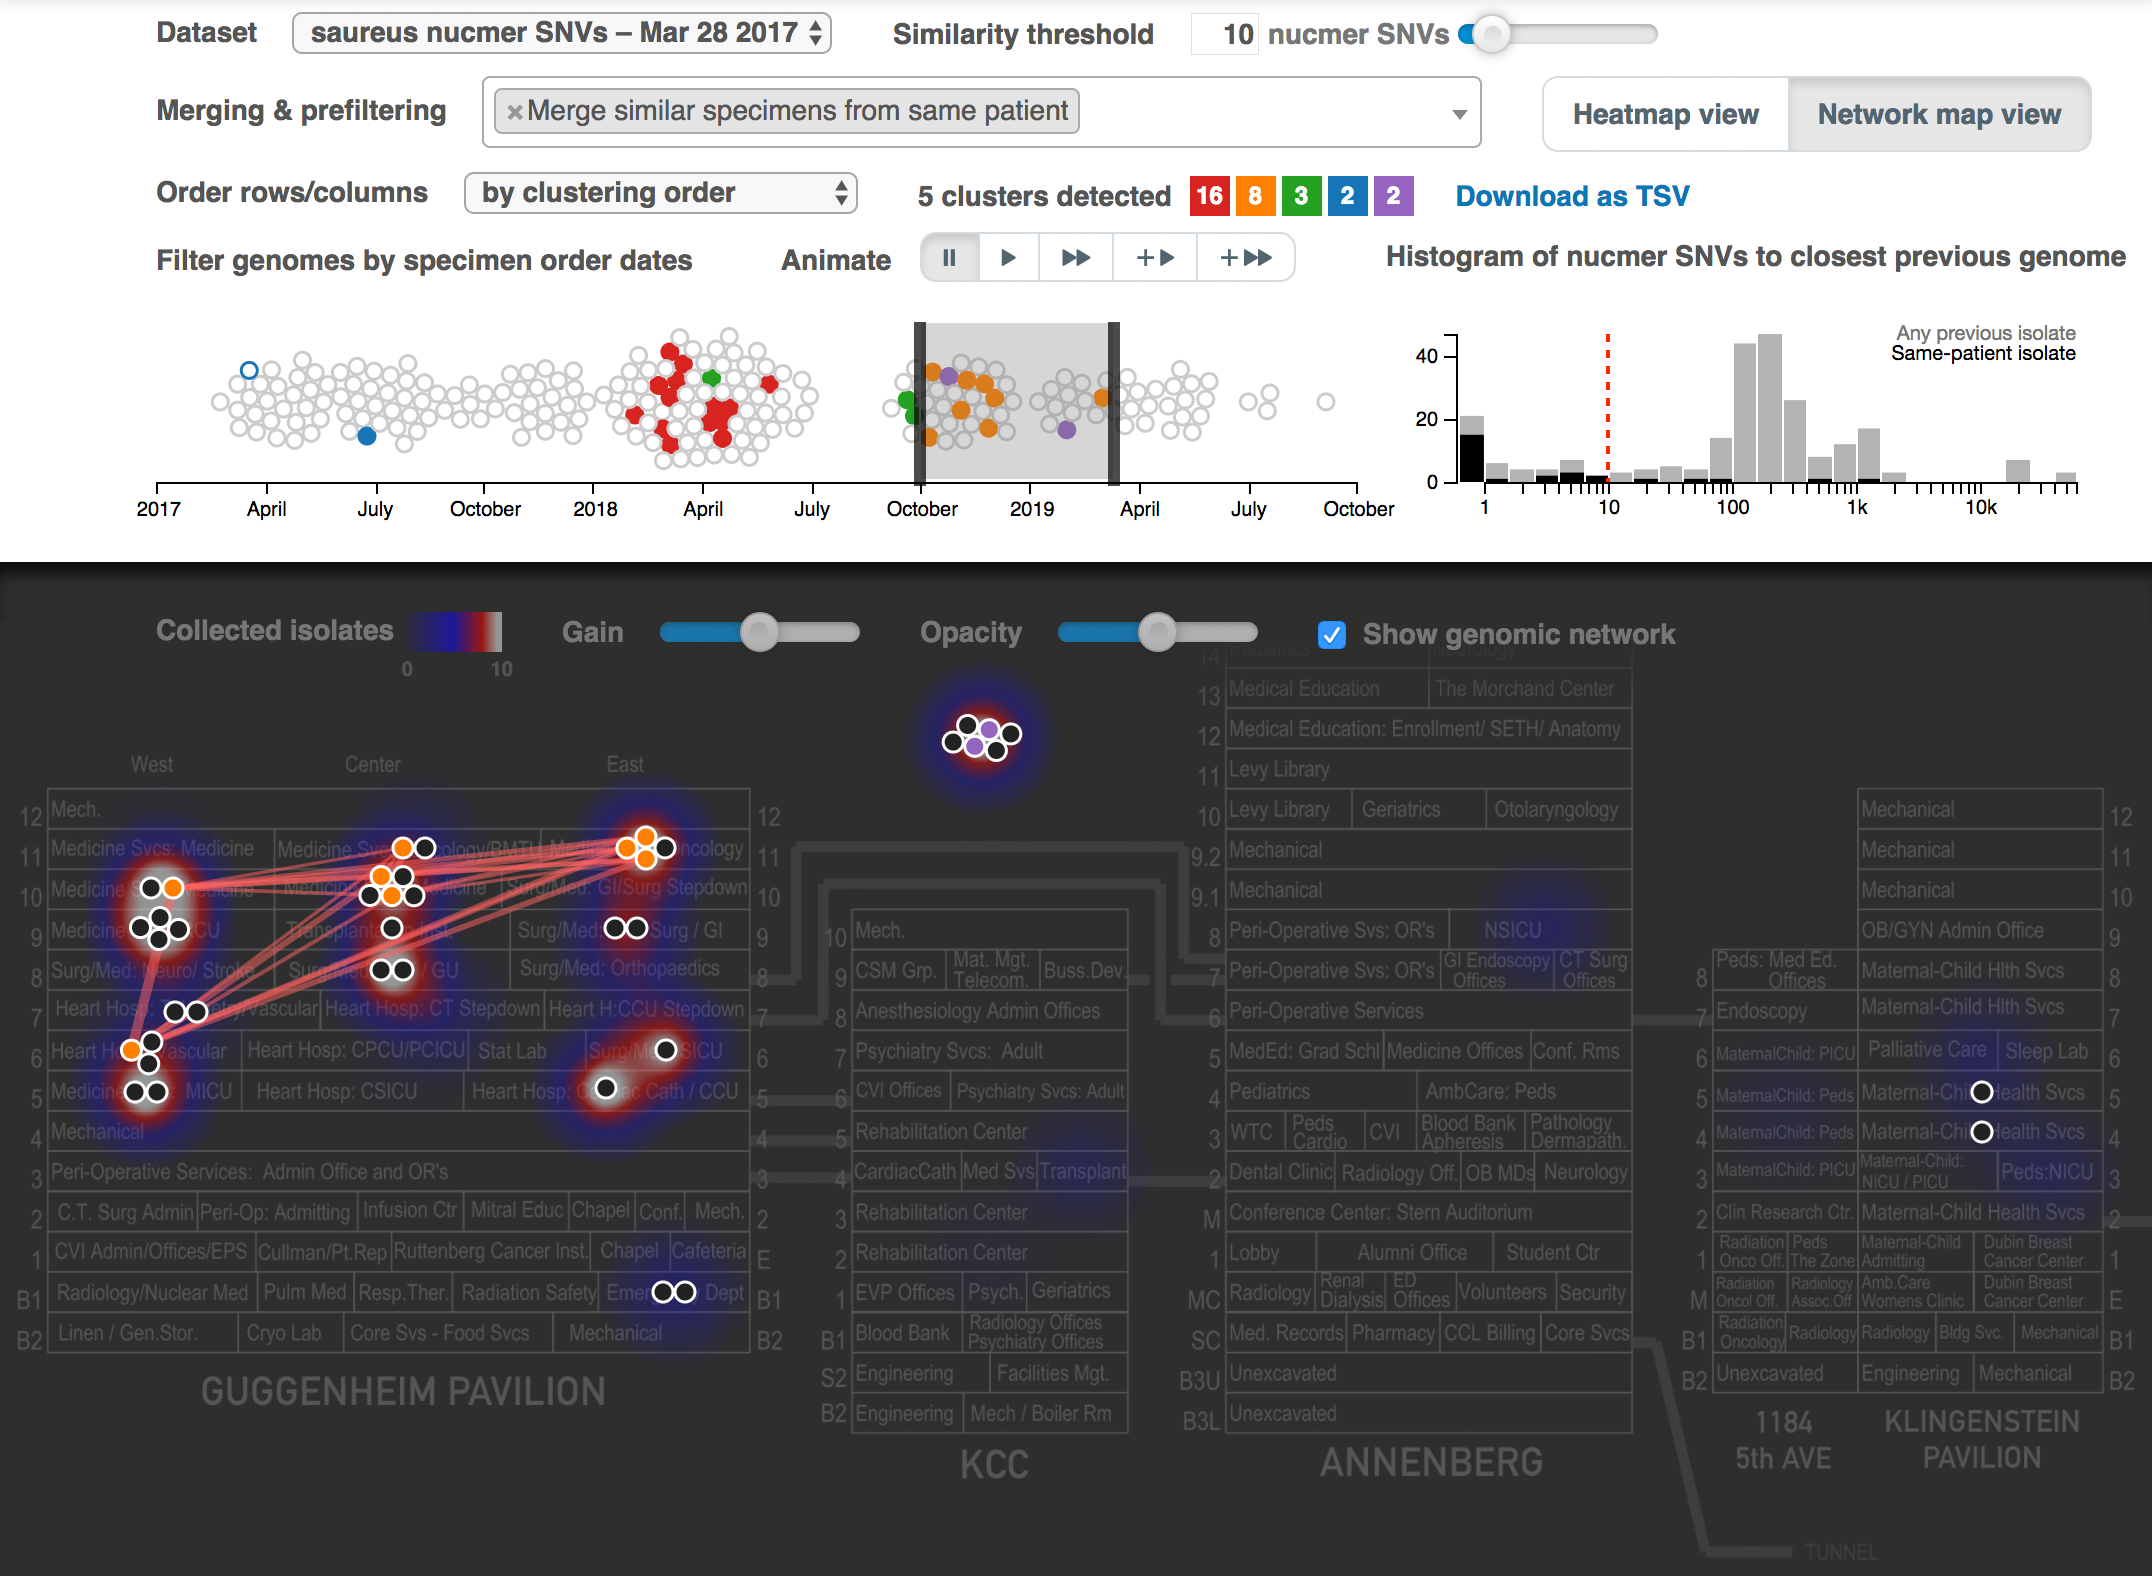
\includegraphics[width=0.9\textwidth]{chap4/pdb-geospatial-saureus}               
  \fullwidthlabelcaption{fig:pdb_geospatial_saureus}{\pathogendbviz{} geospatial visualization for an NGS-confirmed cluster of \emph{S. aureus} isolates}{\textbf{\pathogendbviz{} geospatial visualization for an NGS-confirmed cluster of \emph{S. aureus} isolates.} Note that dates have been shifted into the future to reduce the disclosure of potentially identifying information. The top of the interface is as in Figure \ref{fig:pdb_heatmap_saureus}. At bottom, node-link diagram of putative transmissions, with circles representing sequenced isolates in the selected time range (see timeline beeswarm plot) and red lines connecting isolates underneath the chosen SNV threshold (here, 10 SNVs). Nodes are placed on top of the hospital unit (light gray stacking diagram, vertical axis corresponds to floor level) from which the isolate was collected. The density plot underneath nodes represents the overall frequency of positive cultures at each location of the hospital.}
\end{sidewaysfigure}

\newthought{A spatial layout} can be useful to visualize isolates and their links in relationship to hospital locations, and is provided as an alternative view by \pathogendbviz{} (Figure \ref{fig:pdb_geospatial_saureus}). This interface, which is accessed by toggling the ``Network map view'' button in the upper right corner, has been focused on only the isolates in the time range of the orange cluster, although we now include unrelated isolates as well (note that the beeswarm timeline contains new light gray circles, which are the isolates that were not involved in any putative transmissions). In this view, the isolates are depicted as dots on top of a stacking layout of Mount Sinai's hospital campus, which has several different buildings (see the Building labels at bottom; names anonymized). The floors are laid out vertically in this diagram, and connections between them (like sky bridges) are depicted as thick lines. (The isolates hovering over Building B were sent from a different campus.) Dots are colored by the cluster they were in, and transmissions between patients according to the SNV threshold are drawn as red lines. This diagram makes it apparent that the patients in the orange cluster were spread across the upper floors of the leftmost building, with at most three patients sharing a unit. The spatial network layout also includes a density plot (the fuzzy clouds underneath the points) that depicts all collected isolates in PathogenDB, including those not yet sequenced. Therefore, the density plot can reveal parts of the hospital that had many cases of the HAI, but have been undersampled by the NGS data, and could merit follow-up sequencing of the banked isolates. In the case of Figure \ref{fig:pdb_geospatial_saureus}, there are no clouds without dots, meaning that all ``hot spots'' for \emph{S. aureus} in the hospital during this time interval were at least partially captured in the NGS data.

\subsection{\pathogendbviz{} identifies local diversity and transmissions of \emph{C. difficile}}

\begin{sidewaysfigure}[hp]
  \sidewaysvspace
  \centering
  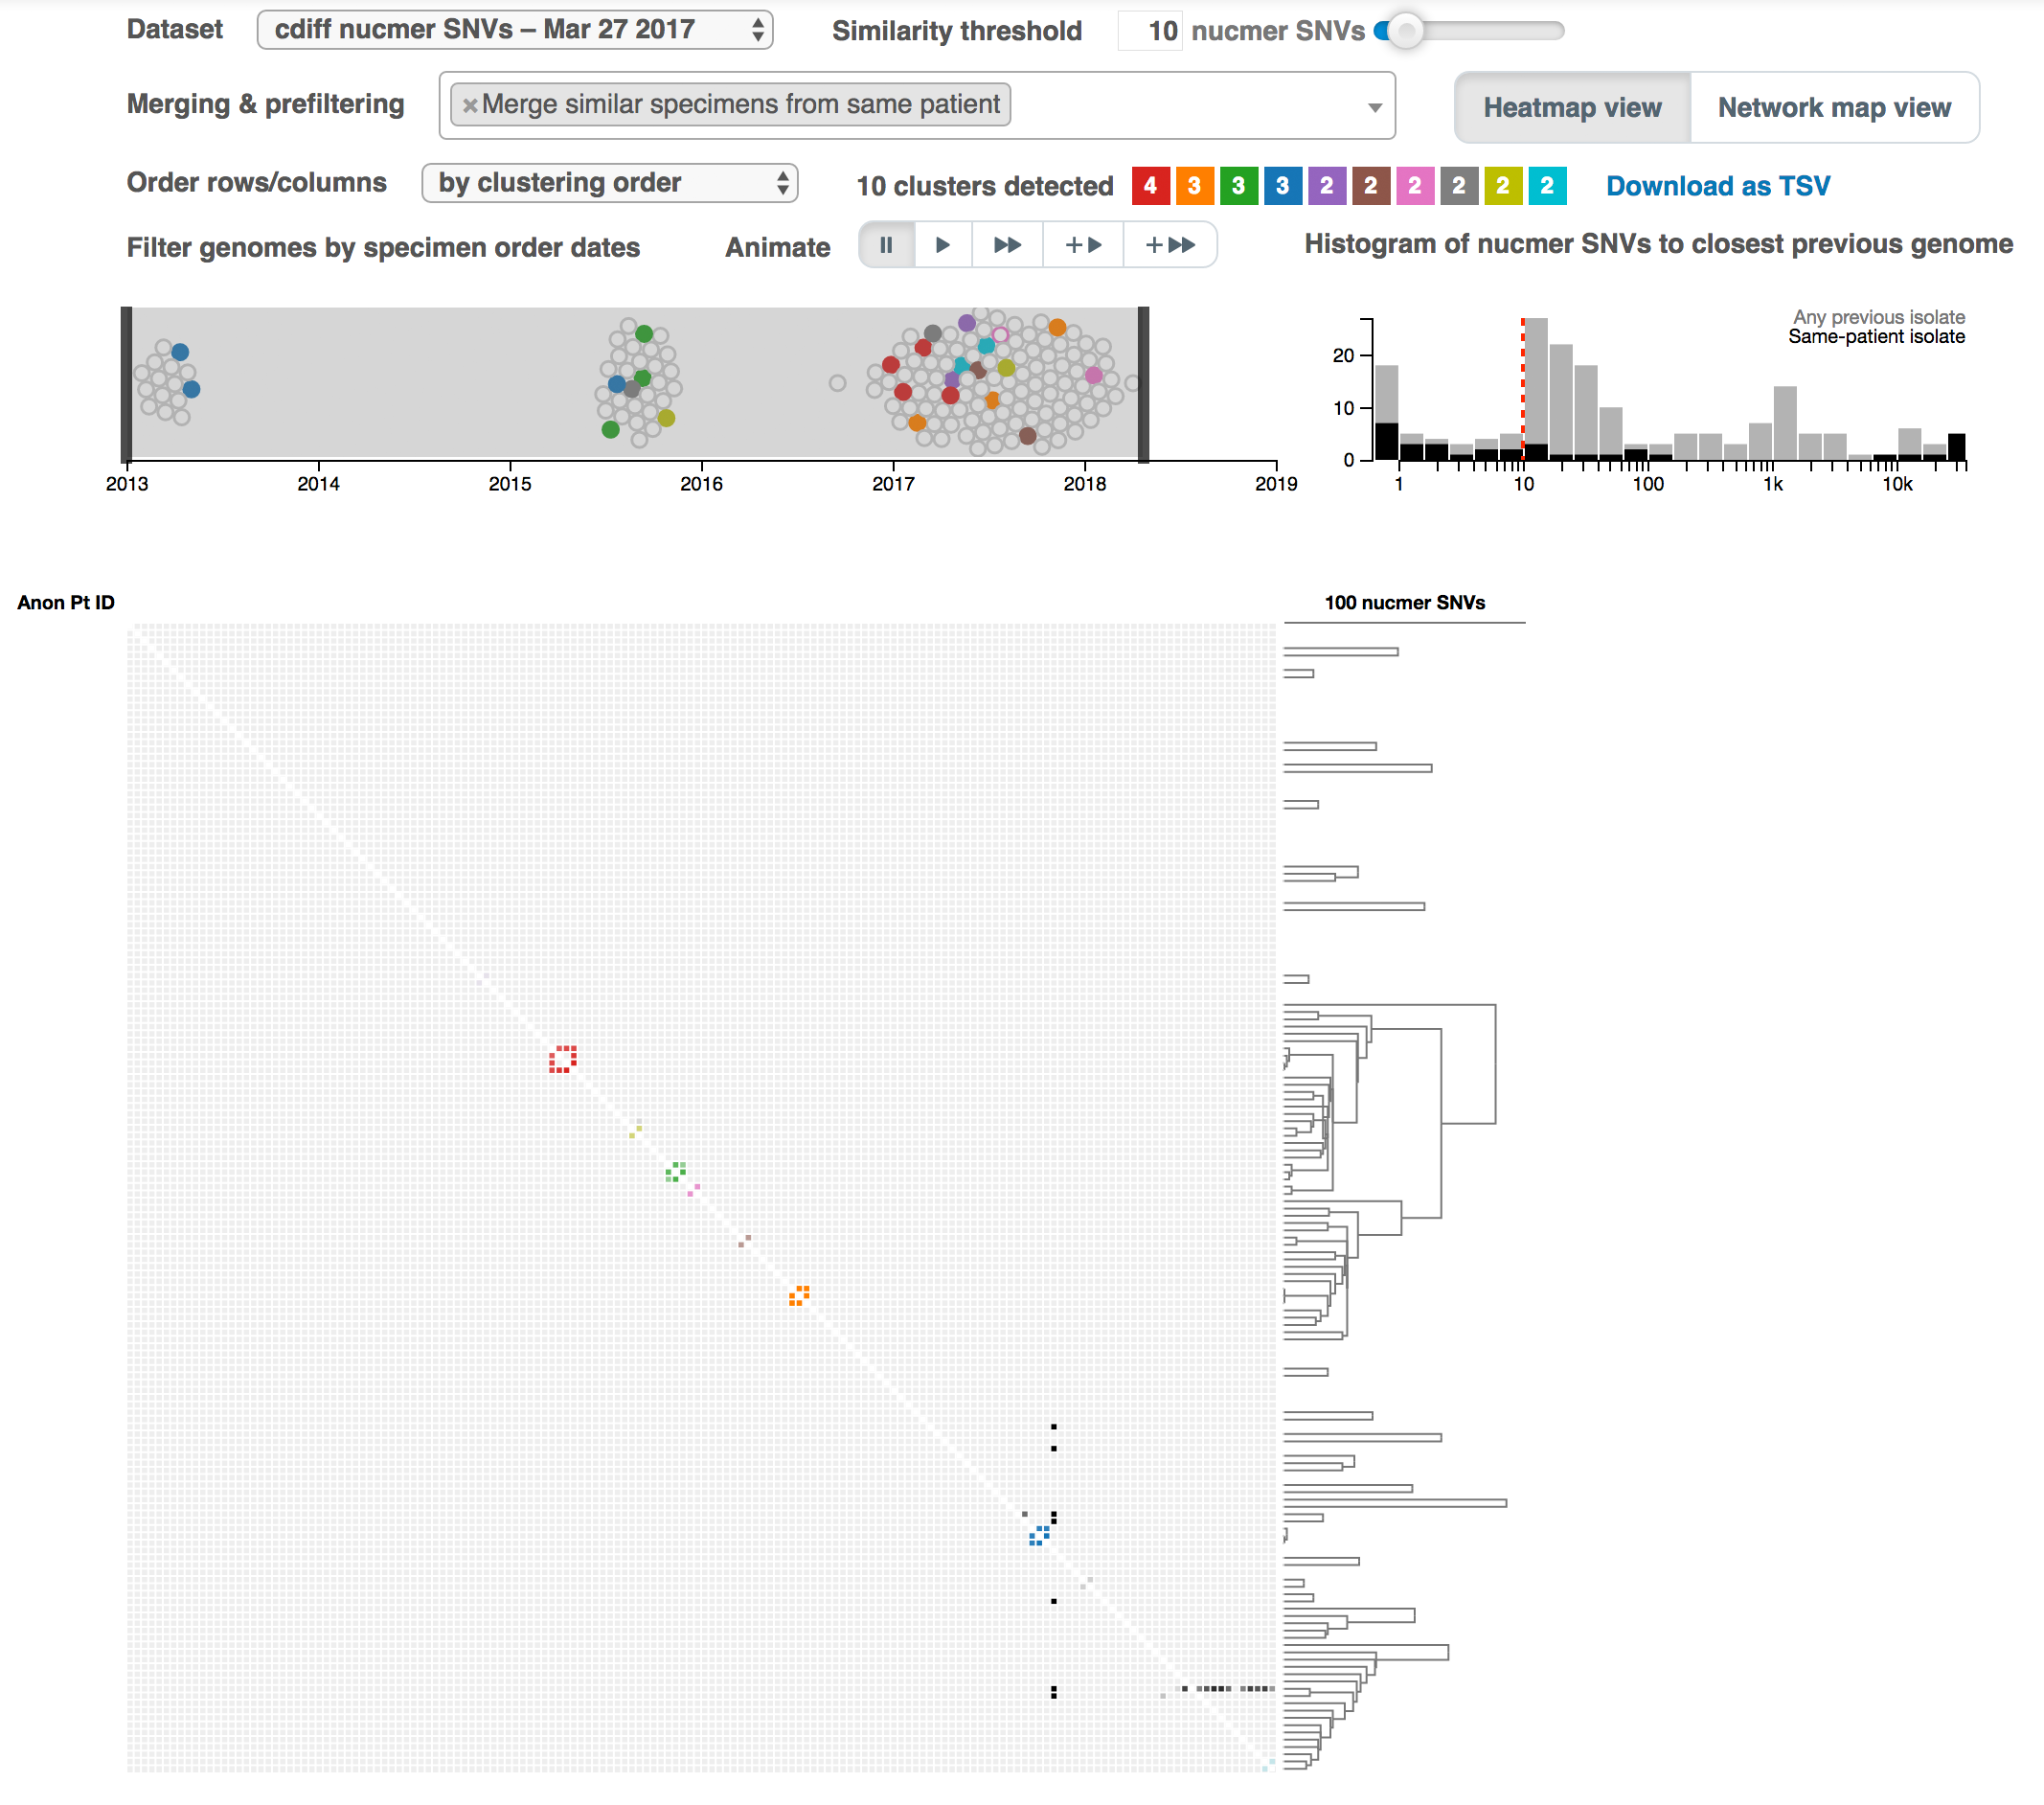
\includegraphics[width=0.8\textwidth]{chap4/pdb-heatmap-cdiff}               
  \fullwidthlabelcaption{fig:pdb_heatmap_cdiff}{\pathogendbviz{} heatmap visualization for all sequenced \emph{C. difficile} isolates over a five-year period}{\textbf{\pathogendbviz{} heatmap visualization for all sequenced \emph{C. difficile} isolates over a five-year period.} All conventions used here are equivalent to Figure \ref{fig:pdb_heatmap_saureus}. Note that dates have again been shifted into the future to reduce the disclosure of potentially identifying information, and we have also censored all sample metadata from this screenshot.}
\end{sidewaysfigure}

We now use \pathogendbviz{} to similarly visualize all sequenced isolates of \emph{C. difficile}. While the Pathogen Surveillance Program has collected all positive \emph{S. aureus} cultures over the past \textasciitilde{}2 years, the surveillance of \emph{C. difficile} has been broader, including sequencing of isolates from pilot periods roughly one year and three years before the start of routine daily collection from all Mount Sinai units \textasciitilde{}1.5 years ago. This is reflected in the trimodal distribution of isolates along the timeline in Figure \ref{fig:pdb_heatmap_cdiff}, where we have included all isolates, not just putative transmissions. We set a similar SNV threshold of 10 SNVs for this longer time period based on the histogram of SNV distances (top right of Figure \ref{fig:pdb_heatmap_cdiff}). Under this threshold, we discover ten small clusters, the largest of which has four patients and with most having only two. Scanning the color of the dots in the timeline indicates that most of the clusters sensibly fall within month-scale intervals, although the yellow-green, gray, and blue clusters are remarkable for spanning the >1 year gaps between the different surveillance periods.

The heatmap visualization at the bottom left of Figure \ref{fig:pdb_heatmap_cdiff} shows the clusters as small groups along the diagonal, and the clustering dendrogram at bottom right shows that some of the clusters separate from each other by distances of \textasciitilde{}20 SNVs.\footnote{Recall the current estimates of the mutation rate for \emph{C. difficile} are around 2-3 SNVs per year; see \textcite{Eyre2013,Eyre2012}.} Therefore, there is certainly some interplay between \emph{C. difficile} evolution in the local community and what eventually arrives at Mount Sinai. What is more notable is that many isolates across the five year capturing period appear to be unrelated (the heatmap is mostly blank). Although constrained by our limited sampling, this is consistent so far with a previous NGS study that concluded that patient-to-patient transmissions were not a major source of hospital-associated \emph{C. difficile} infections over a three-year period in Oxfordshire, United Kingdom.\autocite{Eyre2013}

Note that there are three spurious low SNV distances seen in the upper left of the heatmap (three unclustered black squares) likely caused by a low-quality assembly, which should be re-examined. Low-quality assemblies can appear to have no SNVs if they contain too much redundant sequence, usually caused by duplicate contigs failing to be merged during assembly. Since the heatmap calculates SNV distances in both directions (above and below the diagonal), the lack of an equivalent SNV distance in the reverse comparison provides an easy way to double-check the procedure. This offers some resilience against spurious low SNV transmission predictions caused by misassembled genomes.

\begin{sidewaysfigure}[hp]
  \sidewaysvspace
  \centering
  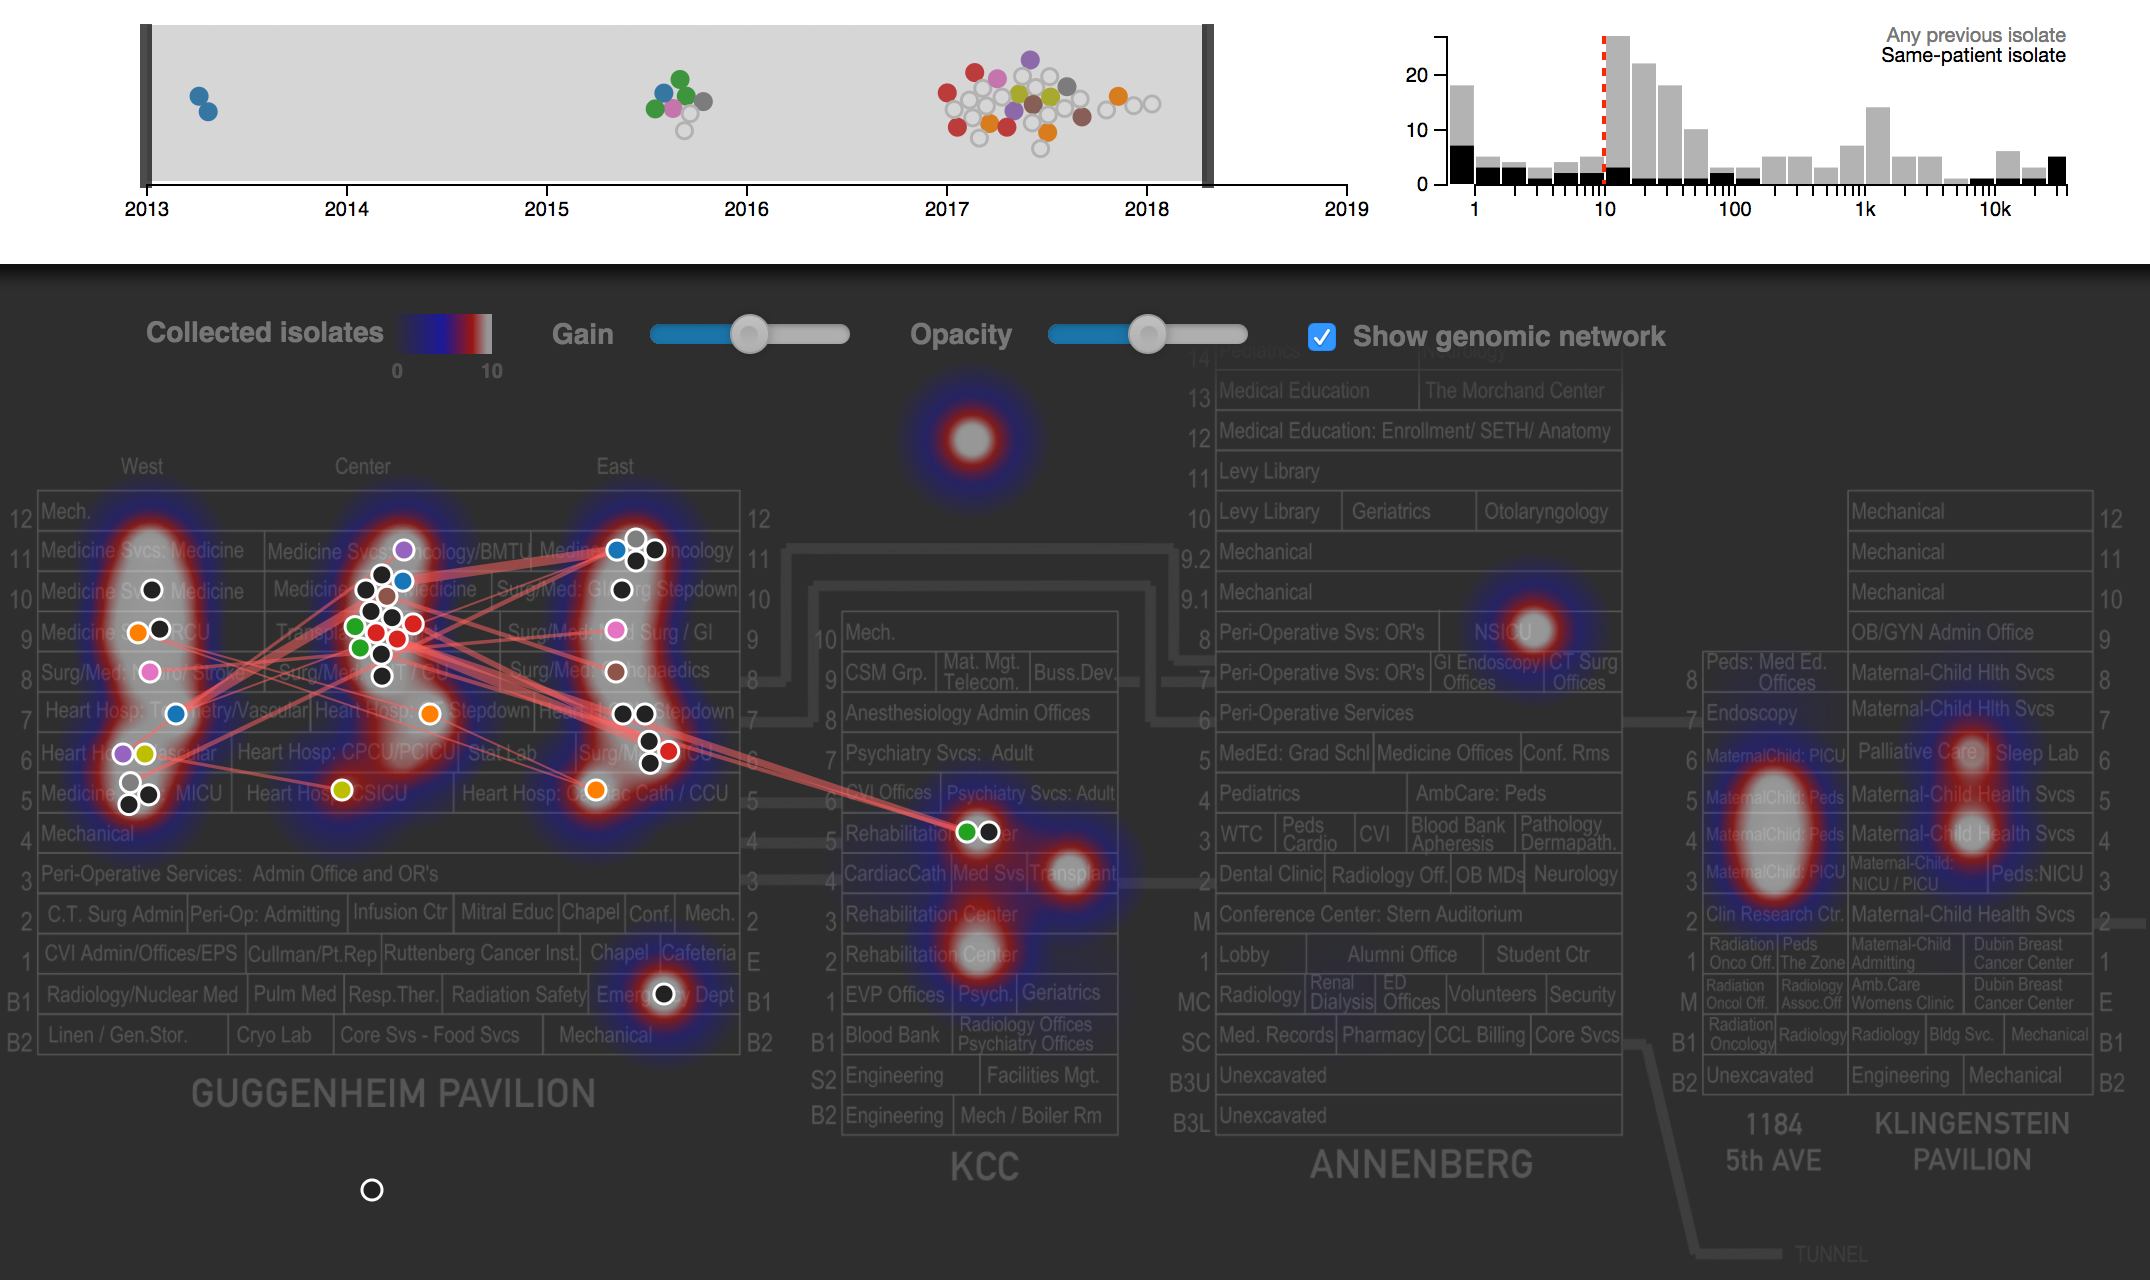
\includegraphics[width=\textwidth]{chap4/pdb-geospatial-cdiff}               
  \fullwidthlabelcaption{fig:pdb_geospatial_cdiff}{\pathogendbviz{} geospatial visualization for NGS-confirmed clusters of \emph{C. difficile} isolates over a five-year period}{\textbf{\pathogendbviz{} geospatial visualization for NGS-confirmed clusters of \emph{C. difficile} isolates over a five-year period.} All conventions used here are equivalent to Figure \ref{fig:pdb_geospatial_saureus}.  Note that dates have been shifted into the future to reduce the disclosure of potentially identifying information.}
\end{sidewaysfigure}

Finally, we can again visualize the spatial relationships among clusters using the network map view in Figure \ref{fig:pdb_geospatial_cdiff}. In this view, which is now focused only on isolates with at least one link to a different-patient isolate, we see that most of the clusters are spread across multiple units (red lines). There are even  NGS-confirmed links between units in different buildings. Although considering all the hypothetical reasons for this pattern is beyond the scope of this chapter, if these transmissions of \emph{C. difficile} spores are occurring with Mount Sinai and not within the community, they are taking places across substantial spatial distances, whether due to movements of patients, visitors, staff, or equipment.

\section{Conclusions}

We have developed a new open-source software suite, PathogenDB, that permits semi-automated epidemiological analysis of HAIs based on long-read sequencing and \emph{de novo} assembly of all isolates. We chose a modular design, separating concerns into a LIMS that centralizes storage of the most up-to-date data, a genome assembly and annotation workflow called \pathogendbpipeline, a comparative genomics toolkit called \pathogendbcomparison, and the visualization tool \pathogendbviz. Thus far,we have assembled and annotated 593 genomes, mostly of \emph{S. aureus} and \emph{C. difficile}, using \pathogendbpipeline{}. This part of the analysis, which is the most computationally intensive, can run in 2-3 hours per isolate on a single server (Figure \ref{fig:pdb_benchmark}) and in >70\% of cases can completely finish the genome assembly without human intervention (Table \ref{tab:pathogendb_assemblies}). We can then integrate phylogenetic and epidemiological analyses into a ``live view'' of putative transmissions mapped to hospital locations, using novel interactive heatmap and network map layout visualizations as implemented in \pathogendbviz.

Our software suite was able to genomically characterize one known MRSA outbreak (red cluster in Figure \ref{fig:pdb_heatmap_saureus}) and discover a previously unknown MRSA outbreak (orange cluster in Figures \ref{fig:pdb_heatmap_saureus}-\ref{fig:pdb_geospatial_saureus}). We have likewise used it to characterize the incidence and spatial distribution of transmissions of \emph{C. difficile} across a surveillance period of five years (Figures \ref{fig:pdb_heatmap_cdiff}-\ref{fig:pdb_geospatial_cdiff}). Addtionally, we used earlier versions of our software to characterize two transmissions via solid organ transplant,\autocite{Altman2014,Bashir2017} and pseudo-outbreaks of \emph{B. cepacia} and \emph{S. maltophilia}.\autocite{Pak2015a} The three modules of the PathogenDB suite are freely available on GitHub (see Availability above) and are being prepared for public use in generic computing environments.

\section*{Notes}

\subsection*{Contributions}

Theodore R. Pak (\smallcaps{TRP}), Mitchell Sullivan (\smallcaps{MS}), Oliver Attie (\smallcaps{OA}), Elizabeth Webster (\smallcaps{EW}), Robert Sebra (\smallcaps{RS}), Camille L. Hamula (\smallcaps{CLH}), Gintaras Deikus, (\smallcaps{GD}), Leah C. Newman (\smallcaps{LCN}), Gopi Patel (\smallcaps{GP}), Deena R. Altman (\smallcaps{DRA}), Shirish Huprikar (\smallcaps{SH}), Ali Bashir (\smallcaps{AB}), Andrew Kasarskis (\smallcaps{AK}), and Harm van Bakel (\smallcaps{HVB}) contributed to this chapter. 

\smallcaps{TRP} wrote the first versions of \pathogendbpipeline, \pathogendbcomparison, and \pathogendbviz. \smallcaps{TRP}, \smallcaps{MS}, \smallcaps{OA}, \smallcaps{HVB}, \smallcaps{AB}, and \smallcaps{EW} have contributed code to the current version of \pathogendbpipeline. \smallcaps{TRP}, \smallcaps{MS}, \smallcaps{OA}, \smallcaps{HVB}, and \smallcaps{EW} have contributed code to the current version of \pathogendbcomparison. \smallcaps{TRP} wrote the current version of \pathogendbviz. \smallcaps{HVB} created and maintains the PathogenDB database. \smallcaps{DRA}, \smallcaps{GP}, \smallcaps{HVB}, \smallcaps{AB}, and \smallcaps{CLH} organized collection of samples. \smallcaps{GD}, \smallcaps{LCN}, and \smallcaps{RS} prepared sequencing libraries and performed sequencing. \smallcaps{CLH} performed culturing and drug susceptibility testing. \smallcaps{TRP}, \smallcaps{MS}, \smallcaps{OA}, \smallcaps{RS}, \smallcaps{EW}, \smallcaps{HVB}, and \smallcaps{AB} performed data analysis. \smallcaps{SH}, \smallcaps{GP}, and \smallcaps{AK} provided institutional support and critical feedback on \pathogendbviz. \smallcaps{TRP} created all figures and wrote the first draft of this chapter.

\subsection*{Funding}

Funding was provided by the Icahn Institute for Genomics and Multiscale Biology at Mount Sinai. \smallcaps{TRP} was supported by the Icahn Institute for Genomics and Multiscale Biology at Mount Sinai and NIH/NIAID (U19-AI118610 and F30-AI122673). Research was also supported by the Office of Research Infrastructure of the NIH under award number S10-OD018522. The content is solely the responsibility of the authors and does not necessarily represent the official views of NIH.

\subsection*{Conflict of Interest}

The authors have no conflicts of interest to disclose.

\subsection*{Acknowledgements}

We thank Timothy O’Donnell, Tavi Nathanson, and members of the clinical microbiology laboratory at Mount Sinai for their contributions. This work was supported in part by the resources and expertise of the Department of Scientific Computing at the Icahn School of Medicine at Mount Sinai.

%% A chapter for my PhD dissertation
%% First author: Theodore Pak
%%
%% Must be included from main.tex.

\chapter{Estimating local costs of \emph{Clostridium difficile} infection using statistical learning and electronic medical records}
\label{chap:cdi_cost}

\begin{quote}
\emph{Reported per-patient costs of \emph{Clostridium difficile} infection (CDI) vary by two orders of magnitude among different hospitals, suggesting that precise, local analyses are needed to guide decision-making. We sought to estimate changes in length of stay (LOS) associated with CDI at one hospital using only automatically extractable electronic medical record (EMR) data and performed a retrospective cohort study of 171,938 visit records spanning a 7-year period. 23,968 variables were extracted from EMR data recorded within 24 hours of each admission to train an elastic net regularized logistic regression model for propensity score matching. To address time-dependent bias (reverse causation), we stratified comparisons by time-of-infection and fit multistate models. The estimated difference in median LOS for propensity-matched cohorts varied from 3.1 days (95\% CI, 2.2–3.9) to 10.1 days (95\% CI, 7.3–12.2) depending on the case definition; however, dependency of the estimate on time-to-infection was observed. Stratification by time to first positive toxin assay, excluding probable community-acquired infections, showed a minimum excess LOS of 3.1 days (95\% CI, 1.7–4.4). Under the same case definition, the multistate model averaged an excess LOS of 3.3 days (95\% CI, 2.6–4.0). Changes in LOS can be extrapolated to a marginal dollar cost per CDI case by multiplying by the average cost of an inpatient-day. We conclude that infection control officers can leverage automatically extractable EMR data to estimate costs of CDI at their specific institution.
}
\end{quote}

\newthought{\emph{Clostridium difficile} infection} (CDI) is the most frequently reported healthcare-associated infection (HAI) in the US\sidecite[-2cm]{Leffler2015} and the major infective cause of nosocomial diarrhea in developed countries,\sidecite[-1.9cm]{Davies2014} incurring billions of dollars in excess medical costs per year.\autocite{Zimlichman2013} Estimates of the per-patient cost of CDI have varied from \$2,871 to \$122,318 due to differences in methodology, patient inclusion criteria, and regional costs.\autocite{Gabriel2014,Ghantoji2010,Zhang2016} Given the high hospital-to-hospital variability of these costs,\autocite{Lofgren2014,Stevens2015} infection control officers, hospital administrators, and clinicians would benefit from estimates tailored to their particular population and healthcare practices. Concretely defining the potential economic savings of CDI prevention would empower stakeholders to prudently choose among the many available validated interventions.\autocite{Dubberke2014a,Katz2013}

Measuring costs within healthcare systems is notoriously difficult (particularly in the US), as many hospitals do not have access to structured, itemized reimbursement data linked to all of their patient medical records.\autocite{Cooper2015} Even the institutions that have informatics capabilities to retrospectively link these data have relied on the curation of select variables and chart review to estimate attributable CDI cost.\autocite{Dubberke2008,Dubberke2014,Greco2015} Nevertheless, electronic medical record (EMR) systems are used by the majority of first-world acute care facilities.\autocite{Gray2011,Henry2016} Part of the rationale for these systems is that hospitals may leverage EMR data for optimal decision-making by inferring causal relationships from raw observations during routine care.\autocite{Dahabreh2014,Etheredge2007,Pak2015} An analysis based on automatically extractable data from an EMR that quantifies preventable hospital costs, such as those attributable to an HAI like CDI, would be of great value in building a continuously learning healthcare system.\autocite{Krumholz2016} EMRs contain many structured fields relevant to this analysis, including: diagnosis codes and lab results demonstrating onset of HAIs; thousands of variables for procedures, problems, and medications that can serve as covariates for adjustment in observational studies; and importantly, the length of stay (LOS) for each visit, which is the primary contributor to excess costs for most HAIs, including CDI.\autocite{McGlone2012,Wilcox1996,Zimlichman2013}

The goal of this study was to generate a robust estimate of local cost associated with CDI using data that are automatically extractable from a typical EMR. We use all available structured data recorded within 24 hours of admission in the EMR—including over 20,000 variables, such as medications reported and administered, abnormal lab values, and problem list entries—to build fully data-driven models for CDI risk using a machine learning algorithm, avoiding the potential bias of preselected covariates and manual chart review. CDI risk models trained on uncurated data from EMRs have already outperformed models that only incorporate variables for known risk factors, indicating that CDI risk may be nuanced in particular care settings.\autocite{Wiens2014} We then use these trained CDI risk models for propensity score matching, which allows estimation of changes in LOS associated with CDI. Most previous studies of CDI cost do not account for the possibility that longer LOS increases the risk of CDI, i.e., reverse causation, and therefore likely overestimate the cost of CDI.\autocite{Mitchell2014,Stevens2015} To adjust for this, we stratify our analysis by the time of CDI diagnosis to find the change in LOS conditional on minimal prior exposure to the hospital environment. Finally, we compare these results to a multistate model of competing time-dependent risks between discharge and the onset of CDI.

\section{Methods}

\subsection{Data source}

\begin{figure}[htb]
  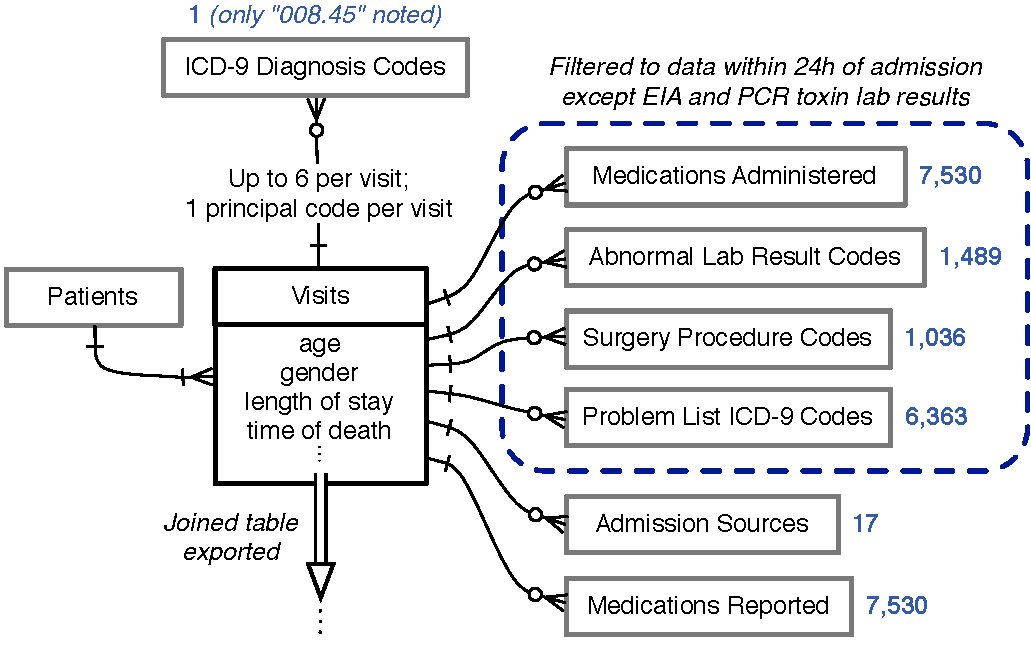
\includegraphics[width=\textwidth]{chap5/1a_methods_db_schema}               
  \caption[Data sources for this study]{\textbf{Data sources for this study}. Entity-relationship diagram for all electronic medical record data used to generate models of \emph{Clostridium difficile} infection propensity, using Information Engineering notation; see \textcite{Halpin2010}. Boxes represent tables of entities with any directly associated attributes (fields) listed below; single lines represent relationships, with arrowheads indicating the cardinality of each side of the relationship; crow’s foot arrowhead with circle represents “zero or more;” crow’s foot arrowhead with cross-stroke represents “one or more;” cross-stroke arrowhead represents “exactly one.” Blue numbers indicate the number of variables extracted from each associated table for each visit. ICD-9, International Classification of Diseases Ninth Revision; EIA, enzyme immunoassay; PCR, polymerase chain reaction.}
  \label{fig:db_schema}
\end{figure}

This study was conducted at The Mount Sinai Hospital, a 1,171-bed tertiary care hospital in New York, NY. Records of adult inpatient visits were extracted from warehoused Epic EMR data and de-identified using the HIPAA Safe Harbor method, 45 CFR §164.514(b)(2). Data was collected on demographics, LOS, time of death, admission sources, reported medications, and the presence of a “008.45” ICD-9 principal or secondary visit diagnosis code denoting “Intestinal infection due to \emph{Clostridium difficile}.” Furthermore, all records of medications administered, abnormal lab result codes, surgery procedure codes, or problem list ICD-9 codes within the first 24 hours after admission were collected as boolean variables (presence or absence). All codes and variables that were uniform across the study population were dropped from the dataset. The relationship between collected data elements, including the maximal cardinality of each datatype, are summarized in Figure \ref{fig:db_schema}. This study was approved by Mount Sinai’s Institutional Review Board as exempt research.

\subsection{Study population}

The cohort included all patients 18 years of age or older admitted between January 1, 2009 and October 22, 2015. For each patient, visits following the first recorded visit in the time range were excluded so that each patient corresponded to a single visit. Visits involving a patient death, defined as a recorded time of death within 24 hours after discharge, were excluded. Visits with missing or invalid date information were excluded (<0.01\% of all records). 

\subsection{Study design}

Prior studies vary on the use of ICD-9 discharge codes vs. positive laboratory tests to define CDI cases\autocite{Gabriel2014,Zhang2016} and identify differing positive predictive values for immunoassay and nucleic acid based laboratory tests.\autocite{Bagdasarian2015,Moehring2013,Polage2015} To ensure maximally robust results and allow comparison with prior studies, we repeated our analysis for five definitions of CDI:

\begin{enumerate}[label=(\roman*),noitemsep,labelindent=2em,leftmargin=!]
\item An “008.45” principal or secondary ICD-9 visit diagnosis code
\item ≥1 positive stool toxin enzyme immunoassay (EIA) lab result
\item ≥1 positive stool toxin polymerase chain reaction (PCR) lab result
\item Either ii or iii
\item Any of i, ii, or iii
\end{enumerate}

Our study’s time range included both a period where the EIA assay was the standard hospital laboratory test (\textasciitilde{}3 years) followed by a period where the PCR assay was standard (\textasciitilde{}4 years). For case cohorts (ii) and (iii), comparisons were only permitted with controls from the time range during which that same test was standard. The hospital laboratory only performs toxin assays on unformed stool samples, implying the presence of diarrhea for positive results.

\subsection{Statistical analysis}

Propensity models for CDI based on the five case definitions were trained using logistic regression with elastic net regularization. Elastic net regularization aims to solve $$\min_{\beta_0,\beta} \frac{1}{N} \sum_{i=1}^{N} w_i l(y_i,\beta_0+\beta^T x_i) + \lambda\left[(1-\alpha)||\beta||_2^2/2 + \alpha ||\beta||_1\right]$$ over a grid of values of $\lambda$, which controls the overall penalization for model size.\footnote{This penalization alleviates the degeneracies of logistic regression when the number of predictor variables $p$ > $N$. FIXME: define other variables.} Here $l(y,\eta)$ is the negative binomial log-likelihood contribution for observation $i$, which is defined as $$y_i \cdot (\beta_0 + x_i^T \beta) - \log (1+e^{(\beta_0+x_i^T \beta)}).$$ The $\alpha$ hyper-parameter, controlling the ratio of $\ell_1$ to $\ell_2$ penalties, was empirically selected on models fit for the first case definition via grid search, maximizing mean area under the receiver operating characteristic curve (AUROC) under five-fold nested cross validation (all values for $\alpha$ ≤ 0.1 produced equivalent AUROCs) and checking for effective shrinkage of coefficients (to within one-fifth of the size of the simplest model). This resulted in selecting $\alpha$ = 0.03. The $\lambda$ hyper-parameter was empirically selected for each modeled case definition by maximizing mean AUROC under five-fold cross validation (Figure \ref{fig:selecting_lambda}).
\begin{figure*}[tbp]
  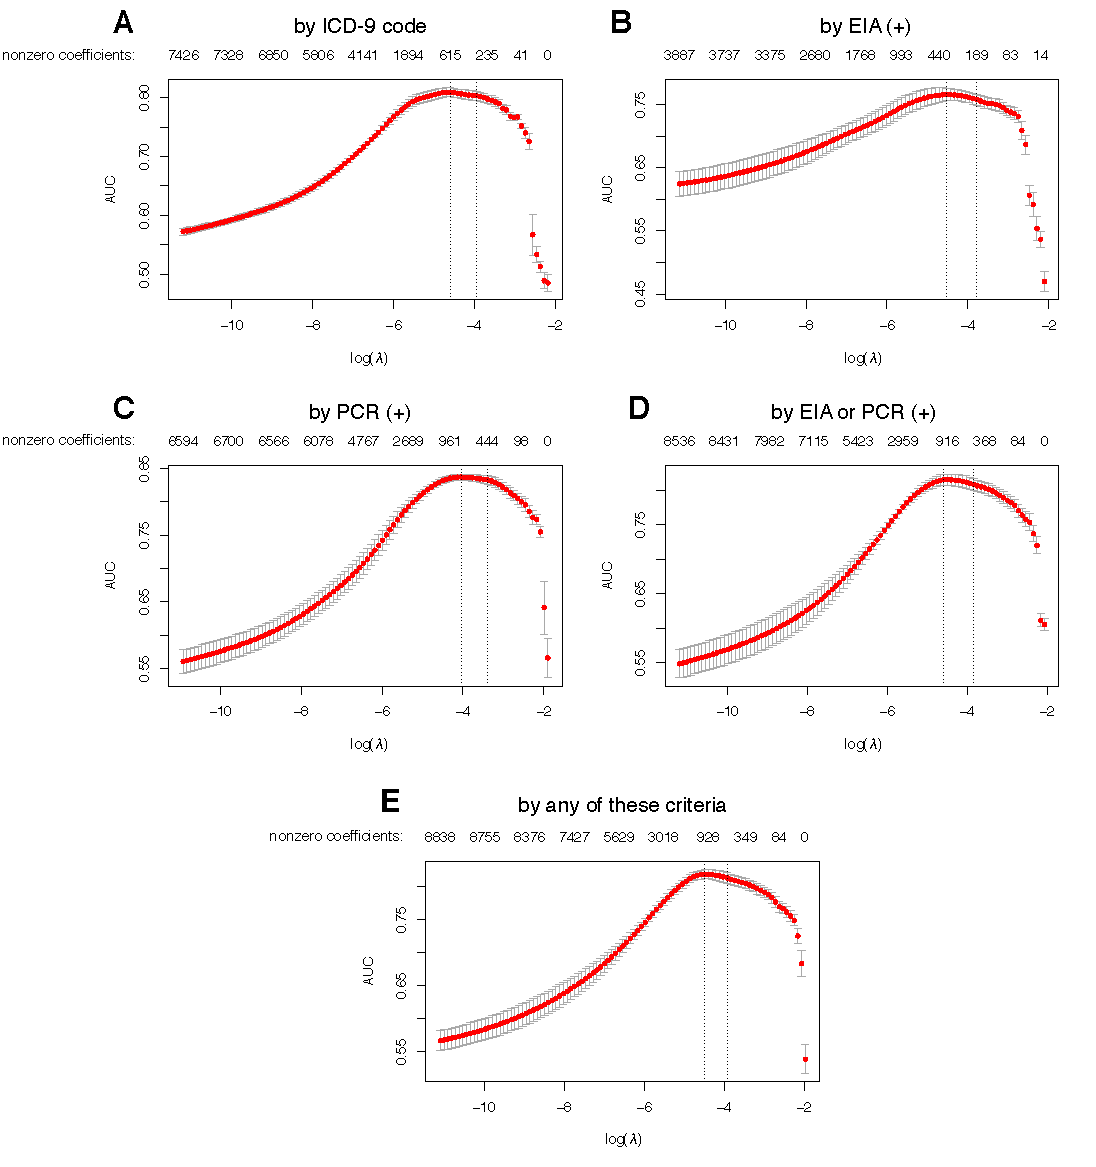
\includegraphics[width=0.9\textwidth]{chap5/S1_selecting_lambda}
  \fullwidthlabelcaption{fig:selecting_lambda}{Selection of the regularization penalty hyper-parameter $\lambda$}{
    \textbf{Empirical selection of the regularization penalty hyper-parameter $\lambda$.} A–E, mean area under the receiver operating characteristic curve (AUC) vs. $\log (\lambda)$ for each of the case definitions for \emph{C. difficile} infection, based on five-fold cross-validation. As the $\log (\lambda)$ penalty hyper-parameter increases, the number of variables left in the model (i.e., with nonzero coefficients) decreases; these are listed across the top of each plot. Vertical bars indicate standard errors. The $\log (\lambda)$ value with maximal mean AUC and the $\log (\lambda)$ value with mean AUC within 1 standard deviation of the maximum are highlighted by vertical dashed lines; the former was used for the final propensity models. ICD-9, International Classification of Diseases Ninth Revision; EIA, enzyme immunoassay; PCR, polymerase chain reaction.
  }
\end{figure*}
Nested cross validation while selecting $\lambda$ was used to evaluate AUROC (which are the performance values reported in Results), while the final propensity models were allowed to see the entire training dataset. 100 bootstrap resampling runs were used to estimate the 95\% AUROC confidence interval (CI). Since propensity models were intended to fairly assess risk at admission for CDI across both cases and controls, variables that could reflect workup or treatment of CDI (as opposed to pre-existing risk) were masked (Table \ref{tab:excluded_vars}). A board-certified infectious diseases physician reviewed the final set of variables selected by each model after regularization\footnote{FIXME: Include in an appendix?} to ensure that none of them reflected medical sequelae of CDI as opposed to potential risk factors.

Matching (1:1) on the propensity score was performed without replacement of controls using a nearest neighbor-matching algorithm and a caliper of 0.2 standard deviations of the logit of the propensity score,\autocite{Austin2011} after exact matching on gender and age divided into six ranges. To assess the performance of the matching, we calculated standardized mean differences\autocite{Austin2011} for age and gender, for which a difference between -0.1 and 0.1 is generally considered negligible,\autocite{Haukoos2015} and examined the distributions of the propensity scores between matched groups.

Furthermore, to ensure that propensity matching itself does not cause spurious changes in the outcome variable (LOS), we repeated the matching algorithm using the matched controls against remaining unmatched controls, creating a “matched-again” control cohort, with the expectation that re-matching controls should not, by itself, create significant differences in the outcome variable. For each case definition of CDI, differences of the median length of stay (LOS) between cases and matched controls were calculated and 95\% CIs were calculated from 10,000 bootstrap resampling runs. The minimum LOS was specified as 0.1 days (2.4 hours), with smaller values rounded up to this value. Statistical significance of differences in LOS was determined using two-sided Mann-Whitney \emph{U} tests. \emph{P} values for all contrasts reported in Figures 2 and 3 are conservatively Bonferroni-corrected for the full number of hypotheses (24). Kaplan-Meier plots were generated to examine the nonparametric maximum likelihood estimation for risk of discharge from the hospital between cases and matched controls, and 95\% CIs for these plots were derived from log-transformed standard errors.

To examine whether changes in LOS may have depended on the time of CDI onset, we repeated the above analysis for case definition (iv) stratified by the time of the first positive toxin assay result, using three ranges: 0–3 days, 3–8 days, and ≥8 days. Propensity models were again fitted to each of these case cohorts for matching as described previously, with the added condition that controls discharged before the start of the CDI time window were ineligible for matching, effectuating simplified balanced risk set matching.\autocite{Li2001} To assess matching performance, propensity score distributions for each group were examined once more, and LOS was analyzed similarly to the original five case definitions.

To further characterize dependence of LOS on the time of CDI onset, we fit a nonparametric multistate model consistent with previous studies.\autocite{Mitchell2014,Stevens2015,VanKleef2014} The model has two transient states (admitted-uninfected and admitted-infected) and one absorbing state (discharged); each patient starts in the admitted-uninfected state. Figure \ref{fig:etm_diagram} is a diagram of all allowed transitions. For all case definitions with a diagnosis time [(ii), (iii), and (iv)], an Aalen-Johansen estimator was used on the full, unmatched dataset to calculate time-varying hazards of each transition. Since the estimator is sensitive to regions with sparsity or outliers, the minimum LOS was specified as 1 day, the time of CDI diagnosis was left- or right-shifted to at least 0.5 days from admission and discharge events, and the model was computed to a precision of 0.1 day up to the 99th percentile LOS value [38.9, 41.9, and 40.9 days for case definitions (ii), (iii), and (iv), respectively]. The mean excess LOS was then estimated as the average difference in LOS between patients with and without CDI at each time t, weighted by the distribution of times spent in the uninfected state. Robust 95\% CIs were generated from 1,000 bootstrap resampling runs.

Analyses were performed in R 3.2.2 (R Foundation for Statistical Computing, Vienna, Austria) using the \texttt{glmnet},\autocite{Friedman2010} \texttt{ROCR},\autocite{Sing2005} \texttt{MatchIt},\autocite{Ho2011} \texttt{survival}, and \texttt{etm}\autocite{Allignol2011} packages. All software code for the analysis is available at: \url{https://github.com/powerpak/cdi-cost}

\section{Results}

371,622 records of visits during the study time range were queried from the EMR, with 23,968 variables extracted for each visit (Figure \ref{fig:exclusions}).
\begin{figure}[htb]
  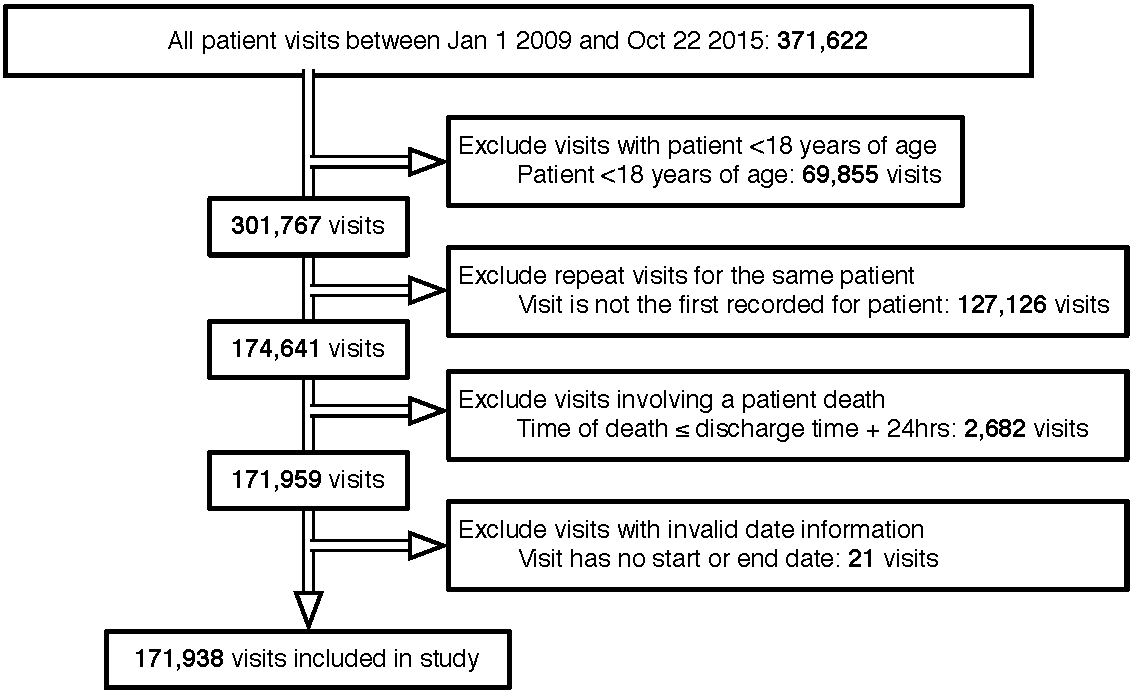
\includegraphics[width=\textwidth]{chap5/1b_methods_exclusion}               
  \caption[Inclusion/exclusion procedure for this study]{\textbf{Inclusion/exclusion procedure for the present study.} Double-line arrows indicate the procession of visit records.}
  \label{fig:exclusions}
\end{figure}
After filtering for the index visit per adult patient and excluding deaths and invalid dates, 171,938 visits were eligible for inclusion and classified into five overlapping case definitions for CDI. Case cohort sizes before matching and overlaps are depicted in Figure \ref{fig:set_intersections}.

\begin{marginfigure}[-4cm]
  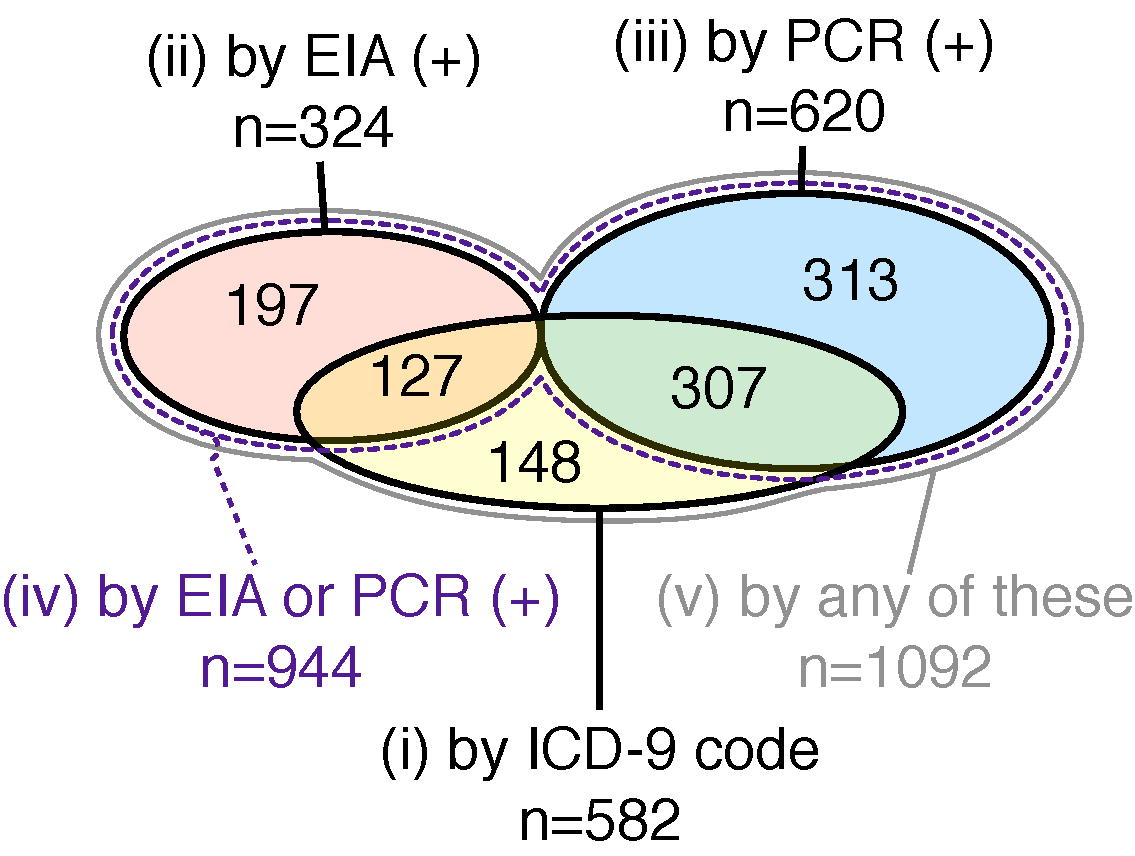
\includegraphics[width=\textwidth]{chap5/S2_set_intersections}               
  \caption[Cohort sizes for each case definition and cohort intersections before matching]{\textbf{Cohort sizes for each case definition and cohort intersections before matching.} Venn diagram of case cohort sizes for each of the five \emph{C. difficile} infection case definitions, before matching, with sizes of all intersections (overlaps) between case definitions. Areas are not to scale. There is no intersection between case definitions (ii) and (iii), since only the first positive toxin assay result for each visit was examined. Case definition (iv), “by EIA or PCR (+),” is a strict superset of case definitions (ii) and (iii). Case definition (v), “by any of these,” is a strict superset of case definitions (i), (ii), and (iii). Sizes of matched case cohorts are provided in Table FIXME.}
  \label{fig:set_intersections}
\end{marginfigure}

\begin{figure*}[tbp]
  \centering
  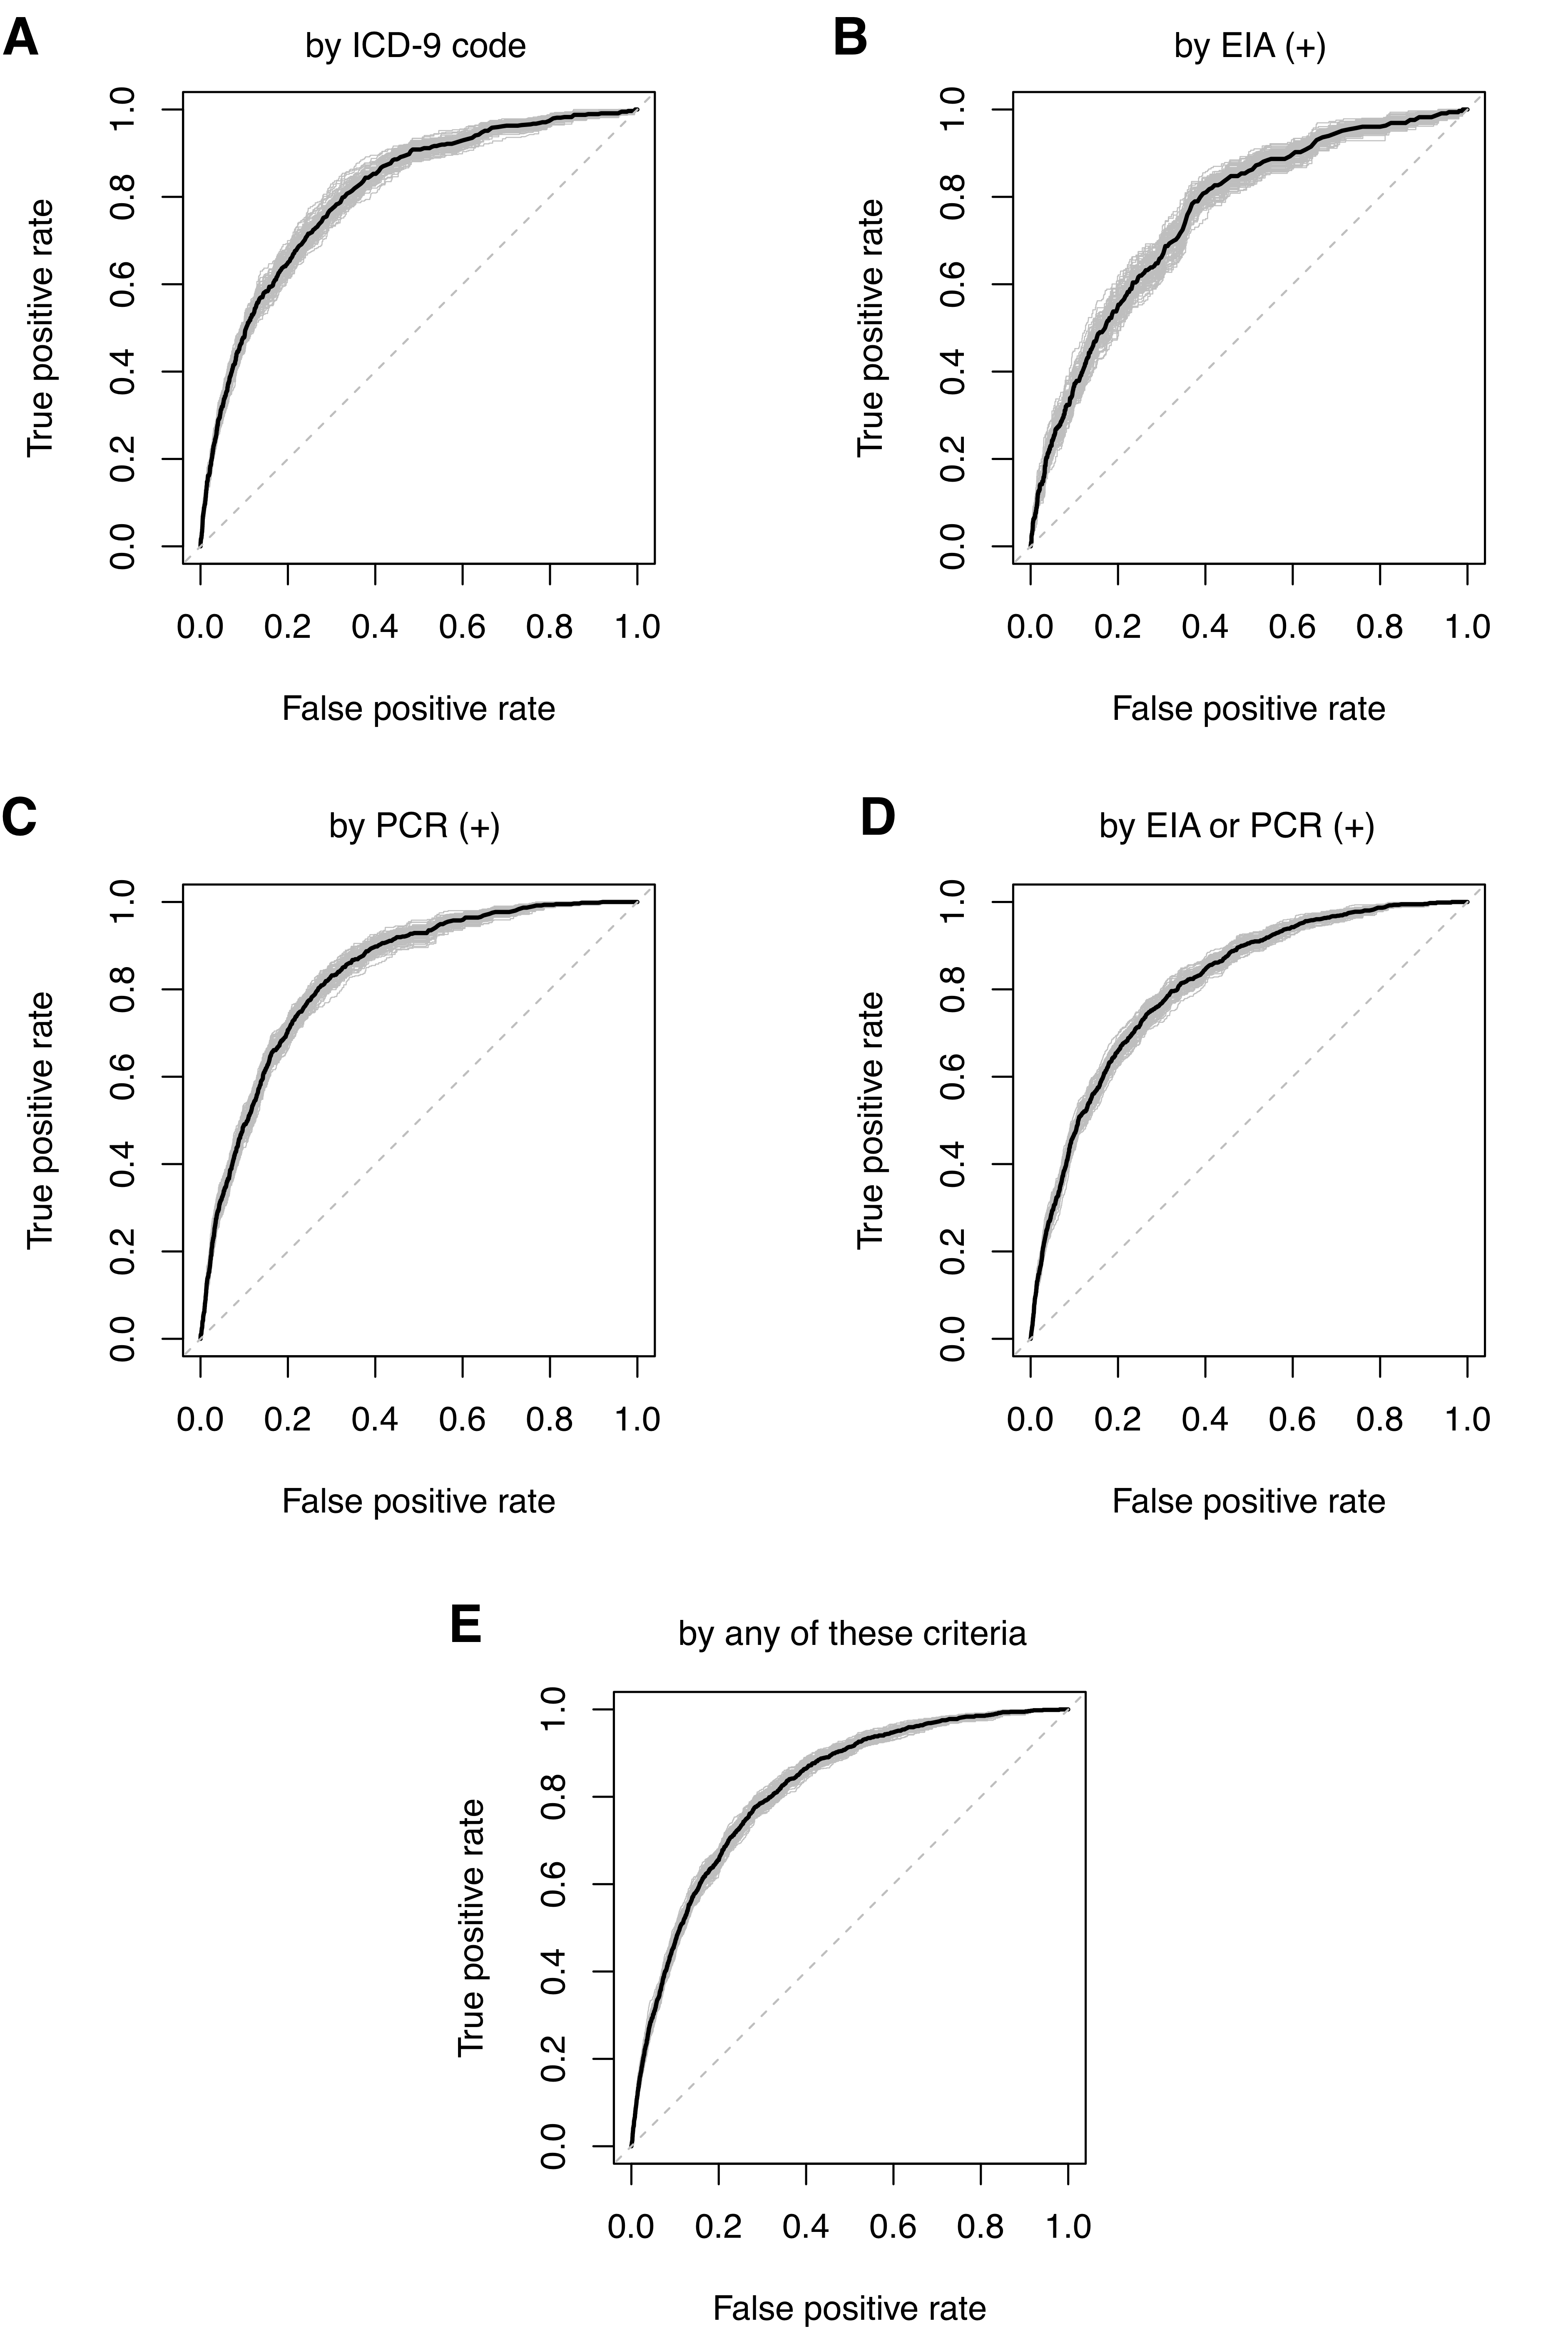
\includegraphics[width=0.7\textwidth]{chap5/S3_ROC}
  \fullwidthlabelcaption{fig:cdi_ROC}{Receiver operator characteristic curves for \emph{C. difficile} infection propensity models}{
    \textbf{Receiver operator characteristic curves for \emph{C. difficile} infection propensity models.} A-E, receiver operator characteristic (ROC) curve comparing the true positive rate against the false positive rate for every possible cutoff of the propensity score, for each of the five \emph{C. difficile} infection case definitions. ROCs are only measured on test data not used to train the models, under five-fold cross validation. Light grey lines indicate ROCs for 100 bootstrap samples. Area under each ROC is reported in the main text under Results. ICD-9, International Classification of Diseases Ninth Revision; EIA, enzyme immunoassay; PCR, polymerase chain reaction.
  }
\end{figure*}

Regularized logistic regression models predicting the risk of CDI acquisition were fit to EMR data from the first 24 hours of each admission for each case definition. The cross-validated mean area under the receiving operator characteristic (AUROC), measuring performance of each model, varied only slightly between case definitions (Figure \ref{fig:cdi_ROC}): (i) by ICD-9 code, 0.81 (95\% confidence interval [CI], 0.79–0.83); (ii) by positive toxin EIA, 0.76 (95\% CI, 0.74–0.78), (iii) by positive toxin PCR, 0.84 (95\% CI, 0.82–0.85), (iv) by either toxin assay, 0.81 (95\% CI, 0.80–0.82); (v) by any of these, 0.82 (95\% CI, 0.81–0.83). The number of selected variables in each model ranged from 373 to 1,027.

\begin{table*}[ht]
  \footnotesize
\begin{flushleft}%
\begin{tabular}{l P{3.15cm} P{1.6cm} P{1.6cm} P{1.2cm} P{1.6cm} P{1.6cm} P{1.2cm}}
  \toprule
  & & \multicolumn{6}{l}{\textbf{Matched cohorts for each CDI case definition}} \\
  \cmidrule(r){3-8}
  & & \multicolumn{3}{l}{(i) by ICD-9 code} & \multicolumn{3}{l}{(ii) by EIA (+)} \\
  \cmidrule(r){3-5}\cmidrule(r){6-8}
  & No. (\%) & \multicolumn{2}{l}{No. (\%)} & & \multicolumn{2}{l}{No. (\%)} & \\
  \cmidrule(r){2-2}\cmidrule(r){3-4}\cmidrule(r){6-7}
  \textbf{Characteristic} &
  All patients (n=171,936) &
  All controls (n=171,356) &
  Matched cases \& controls$^a$ (n=489) &
  SMD after matching (\emph{P} value) &
  All controls (n=73,647) &
  Matched cases \& controls$^a$ (n=274) &
  SMD after matching (\emph{P} value)
  \\
  \midrule
  Female sex & 101,964 (59) & 101,638 (59) & 278 (57) & 0 (1) & 44,132 (60) & 145 (53) & 0 (1) \\
  Age$^b$ \\
  \-\tabindent{}18-29 & 22,344 (13) & 22,266 (13) & 69 (14)   & \multirow{6}{1.5cm}{0.016 (0.86)} &
      9,552 (13) & 22 (8) & \multirow{6}{1.5cm}{0.018 (0.79)} \\
  \-\tabindent{}30-44 & 39,003 (23) & 38,898 (23) &  86 (18)  &  & 16,451 (22) & 26 (9)  & \\
  \-\tabindent{}45-59 & 37,234 (22) & 37,129 (22) &  90 (18)  &  & 15,956 (22) & 58 (21) & \\
  \-\tabindent{}60-74 & 43,946 (26) & 43,802 (26) & 122 (25)  &  & 18,407 (25) & 83 (30) & \\
  \-\tabindent{}75-90 & 26,167 (15) & 26,041 (15) & 106 (22)  &  & 11,817 (16) & 70 (26) & \\
  \-\tabindent{}≥90   &  3,244 (2)  &  3,220 (2)  &  16 (3)   &  &  1,464 (2)  & 15 (5)  & \\
  \bottomrule
\end{tabular}

\vspace{1em}

\begin{tabular}{l P{1.3cm} P{1.2cm} P{1.2cm} P{1.3cm} P{1.2cm} P{1.2cm} P{1.3cm} P{1.2cm} P{1.2cm}}
  \toprule
  & \multicolumn{6}{l}{\textbf{Matched cohorts for each CDI case definition (cont.)}} \\
  \cmidrule(r){2-10}
  & \multicolumn{3}{l}{(iii) by PCR (+)} & \multicolumn{3}{l}{(iv) by EIA or PCR (+)} & 
    \multicolumn{3}{l}{(v) by any of the criteria} \\
  \cmidrule(r){2-4}\cmidrule(r){5-7}\cmidrule(r){8-10}
  & \multicolumn{2}{l}{No. (\%)} & & \multicolumn{2}{l}{No. (\%)} & & \multicolumn{2}{l}{No. (\%)} & \\
  \cmidrule(r){2-3}\cmidrule(r){5-6}\cmidrule(r){8-9}
  \textbf{Characteristic} &
  All controls (n=97,351) &
  Matched cases \& controls$^a$ (n=493) &
  SMD after matching (\emph{P} value) &
  All controls (n=170,994) &
  Matched cases \& controls$^a$ (n=788) &
  SMD after matching (\emph{P} value) &
  All controls (n=170,846) &
  Matched cases \& controls$^a$ (n=945) &
  SMD after matching (\emph{P} value)
  \\
  \midrule
  Female sex & 57,340 (59) & 254 (52) & 0 (1) & 101,469 (59) & 408 (52) & 0 (1) & 101,390 (59) & 493 (52) & 0 (1) \\
  Age$^b$ \\
  \-\tabindent{}18-29 & 12,714 (13) &  47 (10) & \multirow{6}{1.2cm}{0.005 (0.99)} & 
      22,265 (13) & 79 (9) & \multirow{6}{1.2cm}{0.003 (0.98)} &
      22,245 (13) & 87 (9) & \multirow{6}{1.2cm}{0.004 (0.93)} \\
  \-\tabindent{}30-44 & 22,430 (23) &  72 (15) &  & 38,879 (23) & 124 (13) & & 38,845 (23) & 134 (14) & \\
  \-\tabindent{}45-59 & 21,069 (22) & 117 (24) &  & 37,025 (22) & 209 (23) & & 36,999 (22) & 208 (22) & \\
  \-\tabindent{}60-74 & 25,273 (26) & 136 (28) &  & 43,680 (26) & 266 (29) & & 43,643 (26) & 267 (28) & \\
  \-\tabindent{}75-90 & 14,120 (15) & 114 (23) &  & 25,936 (15) & 231 (24) & & 25,912 (15) & 217 (23) & \\
  \-\tabindent{}≥90   &  1,745 (2)  &   7 (1)  &  &  3,209 (2)  &  35 (3)  & &  3,202 (2)  &  32 (3)  & \\
  \bottomrule
\end{tabular}
\end{flushleft}
  \caption[Demographic characteristics of the study population and matched cohorts]{\textbf{Demographic characteristics of the study population and matched cohorts.} Abbreviation: CDI, Clostridium difficile infection; ICD-9, International Classification of Diseases Ninth Revision; EIA, enzyme immunoassay; PCR, polymerase chain reaction; SMD, standardized mean difference. $^a$Separate columns are unnecessary because 1:1 exact matching was performed on the characteristics shown, and therefore all values are identical. $^b$SMD is shown for age treated as a continuous variable; coarsened exact matching was performed using the listed age ranges.
}
  \label{tab:cdi_pts}
\end{table*}

For each case definition, over 75\% of cases were successfully matched by propensity score to controls (Figure \ref{fig:set_intersections} and Table \ref{tab:cdi_pts}). The groups are well matched on demographics and propensity scores (all \emph{P} values >0.1 and standardized differences between –0.1 and 0.1; propensity score distributions in Figure \ref{fig:psm_density}).
\begin{figure}[htb]
  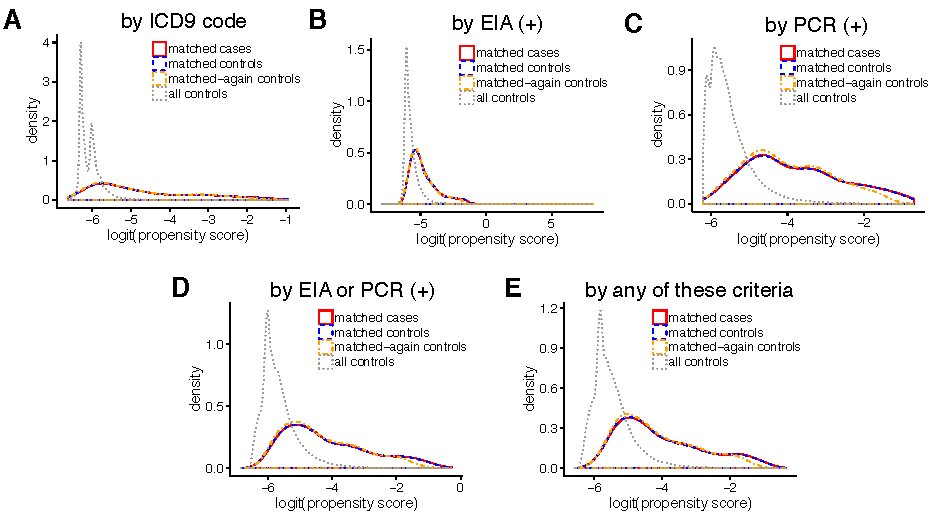
\includegraphics[width=\textwidth]{chap5/S4_psm_density}
  \caption[Propensity score distributions for matched cohorts for each \emph{C. difficile} infection case definition]{
    \textbf{Propensity score distributions for matched cohorts for each \emph{C. difficile} infection case definition.} A-E, density plots of propensity score distributions for matched cases, matched controls, matched-again controls, and all controls for each of the five CDI case definitions. Matched-again controls are derived from a second round of matching between the case-matched controls from the first round of matching and remaining unmatched controls. All X axes are logit-scaled. All Y axes are scaled to unit probabilities; the area under every curve equals 1. The matching algorithm intends to align the propensity score distributions for all of the matched groups.
  }
  \label{fig:psm_density}
\end{figure}
Differences in the median LOS between matched case and control cohorts for all CDI case definitions were strongly statistically significant, although the magnitude of the differences varied greatly between definitions (Figure \ref{fig:violin}). The differences in the median LOS by case definition were: (i) by ICD-9 code, 3.1 days (95\% CI, 2.2–3.9); (ii) by positive toxin EIA, 10.1 days (95\% CI, 7.3–12.2), (iii) by positive toxin PCR, 6.6 days (95\% CI, 5.0–8.1), (iv) by either toxin assay, 7.2 days (95\% CI, 5.8–8.3); and (v) by any of these, 5.7 days (95\% CI, 4.5–6.6). 
\begin{figure}[htb]
  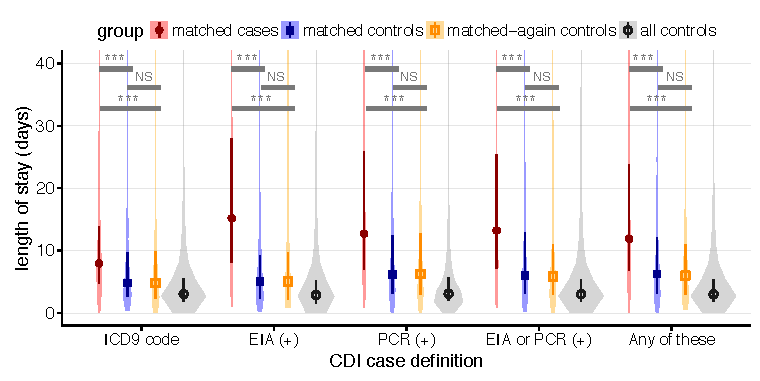
\includegraphics[width=\textwidth]{chap5/2a_violin}
  \caption[Changes in length of stay for five case definitions of \emph{C. difficile} infection, not accounting for time of infection]{
    \textbf{Changes in length of stay for five case definitions of \emph{C. difficile} infection, not accounting for time of infection.} Violin plots of the distributions in length of stay for matched cases, matched controls, matched-again controls, and all controls, for each of the five case definitions. Darker points and vertical bars depict the median and interquartile range for each group. Horizontal bars depict Mann-Whitney \emph{U} tests for significance of differences between groups (***, Bonferroni-corrected \emph{P} < 0.001; NS, not significant [\emph{P} > 0.1]). CDI, \emph{C. difficile} infection.
  }
  \label{fig:violin}
\end{figure}
There were no significant differences in LOS for a second round of matching between matched controls and remaining controls (matched-again controls) for any of the case definitions (Figure \ref{fig:violin}). Kaplan-Meier curves for the time-dependent risk of being discharged from the hospital showed significant differences between matched case and control cohorts up to post-admit day 60 for all case definitions except ICD-9 code (Figure \ref{fig:survival}).

\begin{figure}[htb]
  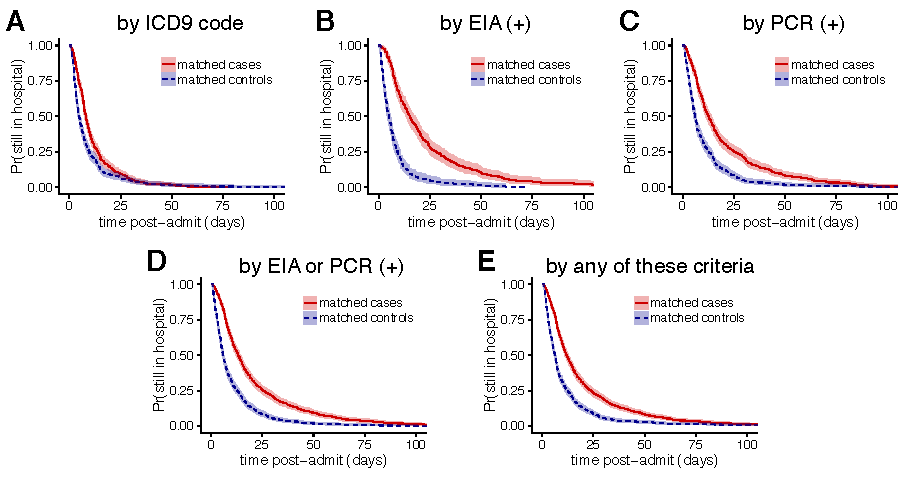
\includegraphics[width=\textwidth]{chap5/2b_survival}
  \caption[Kaplan-Meier plots for length of stay, not accounting for time of infection]{
    \textbf{Kaplan-Meier plots of the time-dependent probability for a patient to still be in the hospital, not accounting for time of infection.} A-E, Kaplan-Meier plots of the time-dependent probability for a patient to still be in the hospital, comparing matched cases and controls for each case definition of \emph{C. difficile} infection. Shaded areas depict 95\% confidence intervals calculated from standard errors. ICD9, International Classification of Diseases Ninth Revision; EIA, enzyme immunoassay; PCR, polymerase chain reaction.
  }
  \label{fig:survival}
\end{figure}

Estimates of LOS associated with CDI are inflated by dependencies on time-to-infection—if longer pre-infection LOS increases CDI risk, i.e., reverse causation, this leads to overestimates in attributable cost.\autocite{Mitchell2014,Stevens2015} We therefore performed two follow-up analyses to account for this. First, we stratified the LOS comparison by the time of CDI diagnosis for case definition (iv) into 0–3 day, 3–8 day, and ≥8 day case cohorts, training new propensity models for another matched comparison, with similar matching performance (Figure \ref{fig:timedep_psm_density}).
\begin{figure}[htb]
  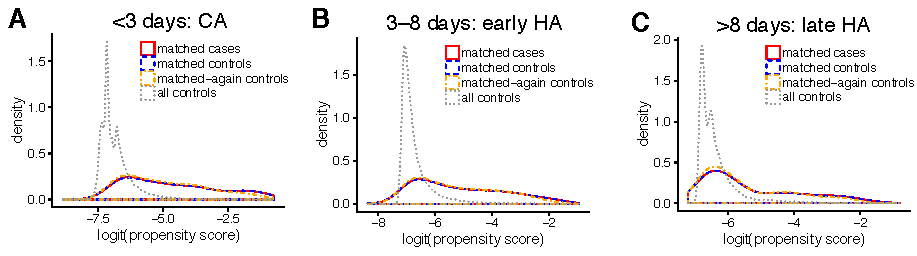
\includegraphics[width=\textwidth]{chap5/S5_timedep_psm_density}
  \caption[Propensity score distributions for matched cohorts stratified by time of \emph{C. difficile} infection diagnosis][-1.5cm]{
    \textbf{Propensity score distributions for matched cohorts stratified by time of CDI diagnosis.} A-C, density plots of propensity score distributions for matched cases, matched controls, matched-again controls, and all controls for cases defined by any positive toxin assay, stratified by the time to infection. Matched-again controls are derived from a second round of matching between the case-matched controls from the first round of matching and remaining unmatched controls. All X axes are logit-scaled. All Y axes are scaled to unit probabilities; the area under every curve equals 1. The matching algorithm intends to align the propensity score distributions for all of the matched groups. CA, community acquired; HA, health- care associated.
  }
  \label{fig:timedep_psm_density}
\end{figure}
Since 3 days (or 72 hours) is a typical cutoff for differentiating community acquired (CA) from healthcare-associated (HA) CDI,\autocite{Longtin2016,Polage2015} these strata were named “CA,” “early HA,” and “late HA,” respectively. As suspected, stratification revealed a positive correlation between time of diagnosis and the CDI-associated difference in LOS (Figure \ref{fig:timedep_violin}). The differences in medians were: for CA, 2.5 days (95\% CI, 1.2–3.4); early HA, 3.1 days (95\% CI, 1.8–4.4); and late HA, 14.0 days (95\% CI, 9.9–17.1). All comparisons between matched cases and controls were again strongly statistically significant, and comparisons between matched controls and matched-again controls were not significant (Figure \ref{fig:timedep_violin}). Kaplan-Meier plots likewise confirmed a correlation between time of CDI diagnosis and the difference in time-dependent discharge risk (Figure \ref{fig:timedep_survival}).

\begin{figure}[htb]
  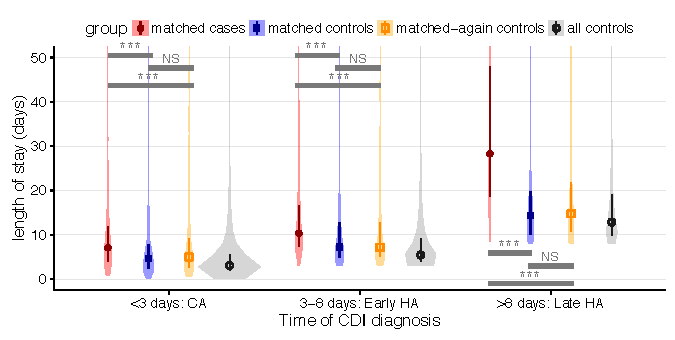
\includegraphics[width=\textwidth]{chap5/3a_timedep_violin}
  \caption[Changes in length of stay for \emph{C. difficile} infection defined by any positive toxin assay and stratified by the time to infection]{
    \textbf{Changes in length of stay for \emph{C. difficile} infection defined by any positive toxin assay, stratified by the time to infection.} Violin plots of the distributions in length of stay for matched cases, matched controls, matched-again controls, and all controls, for three ranges of the result time for the first positive toxin assay. Points and vertical bars depict the median and interquartile range for each group. Horizontal bars depict Mann-Whitney \emph{U} tests for significance of differences between groups (***, Bonferroni-corrected \emph{P} < 0.001; NS, not significant [P > 0.1]). CA, community acquired; HA, healthcare associated.
  }
  \label{fig:timedep_violin}
\end{figure}
\begin{figure}[htb]
  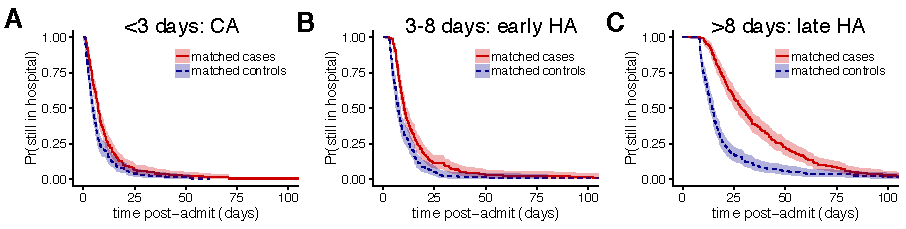
\includegraphics[width=\textwidth]{chap5/3b_timedep_survival}
  \caption[Kaplan-Meier plots for length of stay, stratifying patients by the time to infection]{\textbf{Kaplan-Meier plots of the time-dependent probability for a patient to still be in the hospital, stratifying patients by the time to infection.} A-C, comparison of matched \emph{C. difficile} infection cases and controls for the same three ranges of the time of the first positive toxin assay, stratified by the time to infection. Shaded areas depict 95\% confidence intervals calculated from standard errors. CA, community acquired; HA, healthcare associated.
  }
  \label{fig:timedep_survival}
\end{figure}

To further address reverse causation, we fit a multistate model similar to previously published studies\autocite{Mitchell2014,Stevens2015,VanKleef2014} that explicitly estimates time-dependent, competing risks of transitioning to a CDI-positive state vs. being discharged. Figure \ref{fig:etm_diagram} depicts the three states and allowed transitions of the model. After fitting the model for the case definitions with a time of diagnosis (ii, iii, and iv), the expected remaining LOS can be compared across cohorts that have already transitioned to the CDI infected state vs. those that are still CDI negative at any given timepoint (Figure \ref{fig:etm}).
\begin{marginfigure}
  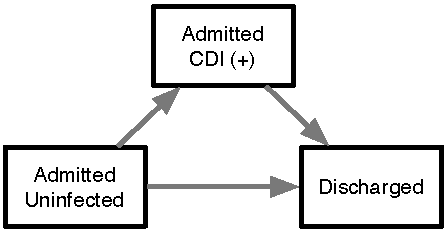
\includegraphics[width=\textwidth]{chap5/4a_etm_diagram}               
  \caption[Multistate model of \emph{C. difficile} infection]{\textbf{Multistate model of \emph{C. difficile} infection.} Three states of the multistate model and allowed transitions. Patients may only transition in the direction of the arrows.}
  \label{fig:etm_diagram}
\end{marginfigure}
To summarize the overall relationship between CDI and LOS, differences in LOS were weighted by the distribution of times spent in the initial state and averaged. The average differences for each case definition were: (ii) by positive toxin EIA, 3.0 days (95\% CI, 2.0–4.0); (iii) by positive toxin PCR, 3.5 days (95\% CI, 2.7–4.5); and (iv) by either toxin assay, 3.3 days (95\% CI, 2.6–4.0). Notably, the 95\% CI for the difference in cohort (iv) overlaps the 3.1 day difference for the “early HA” stratum of the propensity-matched analysis in the same cohort.

\begin{figure*}[htb]
  \centering
  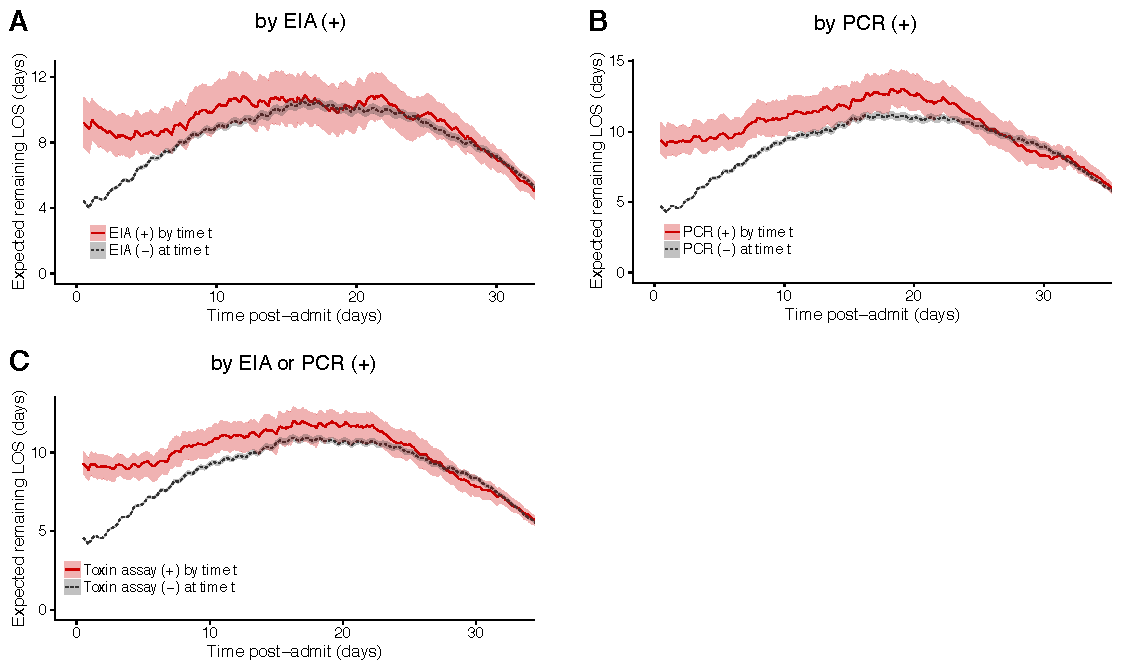
\includegraphics[width=0.8\textwidth]{chap5/4b_etm}
  \caption[Expected remaining length of stay for \emph{C. difficile} infection case definitions as predicted by a multistate model][-4cm]{\textbf{Expected remaining length of stay for \emph{C. difficile} infection case definitions predicted by a multistate model.} A-C, expected remaining LOS for each post-admit time $t$ depending on whether the patient has had a positive (+) toxin assay by that timepoint, for each of the case definitions involving toxin assays. Shaded areas depict 95\% confidence intervals calculated from 1,000 bootstrap samples. CDI, Clostridium difficile infection; EIA, enzyme immunoassay; PCR, polymerase chain reaction; LOS, length of stay.
  }
  \label{fig:etm}
\end{figure*}

\section{Discussion}

This study examined nearly seven years of uncurated EMR data for a single hospital and determined associated costs of CDI as defined by either visit diagnosis codes or lab results. In the analysis unadjusted for time-to-infection, differences in LOS were often greater than national averages from similar unadjusted studies,\autocite{Gabriel2014,Zhang2016,Zimlichman2013} but changes in the case definition resulted in substantial changes in the estimated differences in LOS. Although two hospitals reported good concordance between ICD-9 codes and CDI toxin assay results,\autocite{Dubberke2006,Scheurer2007} this is not necessarily the case for all hospitals. We found that 75\% of ICD-9 coded visits involved a positive toxin assay, while only 46\% of visits with a positive toxin assay had the ICD-9 code (Figure \ref{fig:set_intersections}). Changes in LOS were not significantly different between EIA and PCR toxin assays, although our study was limited by a smaller sample size for EIA (+) cases. Toxin assays are likely a more reliable CDI definition given their basis in clinical symptoms and evidence for CDI, whereas medical coding suffers from biases introduced by billing and reimbursement.\autocite{Rhee2015,Romano1994}

Treating CDI as a baseline condition by ignoring the relationship between pre-infection hospital exposure and CDI risk overestimates associated costs.\autocite{Graves2010,Mitchell2014,Stevens2015} Unlike visit diagnosis codes, toxin assay results provide a presumptive time-to-infection that we incorporated into two different statistical methods addressing time-dependent bias. When using a case definition of either toxin assay being positive, the measured difference in LOS in the multistate model corresponded closely with the difference seen in the “early HA” stratum of a time-stratified propensity-matched analysis (3.3 vs.\ 3.1 days). This suggests that measured differences in this study robustly reflect associated costs of HA-CDI in our patient population. Since estimates for each time-to-infection stratum in the matching analysis differed greatly (Figure \ref{fig:timedep_violin}–\ref{fig:timedep_survival}), time-to-infection clearly contributed bias to the unstratified analysis (Figure \ref{fig:violin}–\ref{fig:survival}), demonstrating how the many studies that ignore this bias\autocite{Gabriel2014,Zhang2016,Zimlichman2013} produce inflated estimates. In our dataset, ignoring time-dependent bias would lead to a more than two-fold overestimation of CDI-associated LOS. Given our findings, we cautiously interpret the results of meta-analyses that conflate ICD-9 code and toxin assay case definitions and often ignore time-dependent bias.\autocite{Gabriel2014,Ghantoji2010,Zhang2016}  

To our knowledge, this is the first study that uses machine learning on uncurated EMR data to estimate the local cost of CDI. Our models of CDI risk performed on par with prior models fitted to lower-dimensional data.\autocite{Dubberke2011,Tanner2009,Wiens2014} Since our models are based on tens of thousands of structured fields in the EMR that require neither chart review nor manual curation beyond masking known CDI-related effects, re-analysis of future data is inexpensive. Starting from exported visit data, the entire analysis runs in several hours on standard desktop computers. Therefore, the effects of new interventions against CDI can be efficiently monitored over time, e.g., continually testing whether new treatments actually lower the CDI-associated LOS or quantifying cost savings of new preventive strategies that decrease CDI incidence. Changes in LOS can be extrapolated to approximate economic costs by multiplying by the average cost of extra inpatient-days as LOS is the main contributor to CDI’s cost.\autocite{Graves2010,McGlone2012,Wilcox1996,Zimlichman2013} In our dataset, using the time-dependency adjusted differences in LOS of 3.1–3.3 days and the national average cost of additional inpatient-days for CDI cases,\autocite{Zimlichman2013} the median cost associated with each case would be approximately \$10,600–11,300; this is substantial in comparison to the national average price for an inpatient visit—approximately \$13,000 in 2011.\autocite{Cooper2015} Using the average yearly caseload observed in the dataset for toxin assay positive cases, our figures represent an annual accounting cost to Mount Sinai of approximately \$1.5 million, not including the opportunity cost of bed occupancy by CDI patients or the impact on infection control resources.\autocite{Graves2010} In principle, our analysis is generalizable to any HAI where lab results recorded in the EMR robustly reflect the incidence of infections.

Our study has several limitations. The analysis was designed with conservative assumptions, preferring that the models underestimate rather than overestimate changes associated with CDI. For example, restricting to one index visit per patient certainly excluded many repeat visits for recurrent CDI, which are known to incur higher costs.\autocite{Dubberke2008,Dubberke2014,Rodrigues2016} We preferred a relatively simple machine learning technique, elastic net regularized generalized linear models, because of its transparency in variable selection and unparalleled speed on sparse training data. More advanced techniques might marginally improve propensity model accuracy at the expense of computational complexity and model interpretability. EMR data has known drawbacks compared to clinical research data, such as limitations in time precision, the sparsity of the data, and increased opportunity for coding error. Also, retrospective matching-based studies face known trade-offs in estimating actual effects of HAIs,\autocite{Graves2010} so we used two separate statistical approaches to control for time-dependent bias, ultimately finding congruous results. We did not have structured billing data, so we cannot trace itemized costs and characterize the exact relationship between LOS and costs beyond the proportional estimate above. Finally, only one hospital’s data was used to implement this analysis, which would benefit from comparison to other hospitals’ data. Therefore, we provide complete code for our analysis so that it may be re-implemented elsewhere and improved by the community.

\section{Conclusions}

\newthought{Two independent} statistical analyses adjusting for time-dependent bias produced similar results for the CDI-associated change in LOS at Mount Sinai (3.1 and 3.3 days), suggesting that automated methods based on machine learning and uncurated EMR data robustly and conservatively estimate the local cost of an HAI in both LOS and financial terms. This procedure is transparent, reproducible, and inexpensive, suggesting that hospitalists and infection control officers can leverage EMR data to estimate their specific, local costs of HAIs on an ongoing basis rather than relying on widely varying benchmarks published by other institutions.

\section*{Notes}

\subsection*{Contributors}

Theodore Pak (\smallcaps{TRP}), Kieran Chacko (\smallcaps{KC}), Timothy O'Donnell (\smallcaps{TO}), Shirish Huprikar (\smallcaps{SH}), Harm van Bakel (\smallcaps{HVB}), Andrew Kasarskis (\smallcaps{AK}), and Erick R. Scott (\smallcaps{ERS}) contributed to this study. \smallcaps{TRP}, \smallcaps{KC}, \smallcaps{AK}, and \smallcaps{ERS} designed the study and developed the models. \smallcaps{TRP}, \smallcaps{KC}, \smallcaps{TO}, \smallcaps{SH}, \smallcaps{HVB}, \smallcaps{AK}, and \smallcaps{ERS} acquired the data. \smallcaps{TRP} performed the data analysis and created all figures in this chapter. \smallcaps{SH} reviewed selected variables for the propensity model. \smallcaps{TO} provided technical support, and \smallcaps{HVB}, \smallcaps{SH}, and \smallcaps{AK} provided administrative and material support. \smallcaps{AK} and \smallcaps{ERS} supervised the study. \smallcaps{TRP} wrote the first draft of this chapter. \smallcaps{TRP} is the first author on the corresponding submitted manuscript.

\subsection*{Funding}

This work was supported by the Icahn Institute for Genomics and Multiscale Biology at Mount Sinai, and also in part by the NIH/NIAID grants F30-AI122673 (\smallcaps{TRP}), T32-GM007280 (\smallcaps{TRP}), and R01-AI119145 (\smallcaps{HVB}, \smallcaps{KC}).

\subsection*{Conflict of Interest}

The authors have no conflicts of interest to disclose.

\subsection*{Acknowledgements}

This work was supported in part by the resources and expertise of the Department of Scientific Computing at the Icahn School of Medicine at Mount Sinai. We thank Deena Altman, Camille Hamula, and Gopi Patel for their assistance in improving the design of the study and reviewing the manuscript.
%% A chapter for my PhD dissertation
%% First author: Theodore Pak
%%
%% Must be included from main.tex.

\chapter{Integrating mass cytometry and transcriptomics into a comprehensive profile of chikungunya infection}
\label{chap:chik}

\hyphenation{Wi-ki-Path-ways Wil-cox-on strong-ly}
\newcommand{\subcommunity}{sub-\allowbreak com\-mu\-ni\-ty}
\newcommand{\subcommunities}{sub-\allowbreak com\-mu\-ni\-ties}
\newcommand{\Subcommunities}{Sub-\allowbreak com\-mu\-ni\-ties}
\newcommand{\pertranscript}{per-\allowbreak trans\-cript}

\begin{quote}
\emph{Chikungunya virus (CHIKV) is a globally epidemic mosquito-borne alphavirus causing acute and chronic arthritic disease. Our study used a systems immunology approach by incorporating whole blood RNA-seq, 35-plex mass cytometry of PBMCs, and serum cytokine measurements of acute and convalescent phase samples from 42 natural pediatric infections in Nicaragua. Semi-supervised classification and clustering of single-cell events into 57 \subcommunities{} of canonical leukocyte phenotypes revealed a monocyte-driven response to acute infection, with greatest expansions of “intermediate” CD14\sups{++}\allowbreak CD16\sups{+} monocytes and an activated subpopulation of CD14\sups{+} monocytes. Increases in acute phase CHIKV surface protein expression were highest for monocytes and dendritic cells, although surprisingly, B cell subpopulations also displayed significant increases. Serum cytokine measurements confirmed significant acute phase upregulation of monocyte chemoattractants. Transcriptomic signatures were revealed not only for infection phase, but also for convalescent phase immunogenicity, acute phase viremic load, and symptom severity. Finally, we present a multiscale network that summarizes all observed modulations across cellular and gene expression levels and their interactions with clinical outcomes, providing a uniquely global view of the biomolecular landscape of CHIK pathophysiology.}
\end{quote}

\newthought{Chikungunya} (CHIKV) is a re-emerging mosquito-borne alphavirus that causes endemic and explosively epidemic infections throughout tropical regions of the world.\autocite{Weaver2015} Transmittable by \emph{Aedes egypti} and \emph{Aedes albopictus}, the same vectors as Dengue virus (DENV), phylogenies of CHIKV have indicated that urban endemic strains originated from several transmission events out of enzootic, sylvatic cycles between non-human primates and arboreal mosquitos in eastern Africa.\autocite{Volk2010} In 2004, the largest outbreak ever recorded spread rapidly from Africa through the Indian Ocean and Asia to Papua New Guinea and islands in the Pacific; subsequently, the first autochthonus transmissions in the Americas and the US were reported in 2013.\autocite{Nasci2014} Millions of cases have now been reported in at least forty countries.\autocite{Suhrbier2012}

Unlike other arboviral diseases like DENV, the majority of CHIKV infections produce symptomatic illness, with typical manifestations consisting of fever, a diffuse body rash, and joint pain and inflammation.\autocite{Couderc2015,Weaver2015} Notably, debilitating joint-related symptoms can persist for years mimicking rheumatoid arthritis in up to 50\% of afflicted populations—the namesake characteristic of the disease, as “chikungunya” is a Swahili/Makonde word describing a bent posture.\autocite{Miner2015,Weaver2015} Rarely, complications can occur, including encephalopathy and encephalitis, fulminant hepatitis, and myocarditis.\autocite{Rolph2015} Mortality occurs in approximately 0.1\% of cases.\autocite{Rolph2015} Besides anti-inflammatories for symptomatic relief, there are no specific treatments available for CHIKV.\autocite{Suhrbier2012,Weaver2015} Several vaccine candidates have reached preclinical or phase I trials,\autocite{Plante2015,Weger-Lucarelli2014} but major commercial investment will be required to complete their development, and finding clinical sites to demonstrate efficacy will be complex because of the unpredictable incidence and spread of the virus.\autocite{Weaver2015} Until a vaccine or antiviral agent is available, prevention efforts will remain focused on mosquito control.\autocite{Weaver2015}  

Because of CHIKV’s recent re-emergence in the Western hemisphere, there are profound gaps in the understanding of CHIKV pathogenesis, including uncertainty over the roles of viral proteins and the myriad genetic and signaling factors involved in a successful or unsuccessful immune response,\sidecite[-1cm]{Assuncao-Miranda2013,Sourisseau2007,Weaver2015} particularly in pediatric cases.\autocite{Teng2015} CHIKV can infect many cell types, including skin fibroblasts, endothelial cells, primary epithelia, and human muscle satellite cells.\autocite{Couderc2015,Lum2015} Reports of tropism in subsets of peripheral blood monocytes (PBMCs) vary, with CHIKV antigens detected in monocytes during acute infection,\autocite{Her2010} although primary monocytes and macrophages only appear to be infectable at low efficiency in vitro.\autocite{Sourisseau2007,Teng2012a} Thus far, primary B and T cells have not been successfully infected in vitro.\autocite{Her2010,Sourisseau2007,Teng2012a} Monocytes and macrophages are thought to have a substantial role in the acute inflammatory response to CHIKV, as primate models show recruitment of these cell types and natural killer (NK) cells to infected tissues,\autocite{Labadie2010} and mouse models treated with bindarit (an inhibitor of monocyte chemoattractant CCL2) showed reduced monocyte recruitment, joint swelling, and bone loss following infection.\autocite{Chen2015,Rulli2011} The role of monocytes appears to be protective as well as inflammatory. For example, mice deficient for CCR2 (the receptor for CCL2) show prolongation of arthritic disease corresponding with replacement of the monocyte/macrophage infiltrate in infected joints by neutrophils and eosinophils.\autocite{Poo2014} In humans, however, details of the relationship between monocyte subpopulations, acute phase pathogenesis, and chronic symptomatology remain poorly understood.\autocite{Burt2017,Weaver2015}

The innate immune response, particularly via type I interferon (IFN) signaling, is important for control of CHIKV replication during the acute phase of infection.\autocite{Burt2017,Schilte2010} CHIKV infection acutely induces high levels of IFNα release in both humans and model organisms.\autocite{Labadie2010,Teng2015} In mouse models, type I IFNs control CHIKV replication by directly acting on nonhematopoietic cells, likely via activation of host sensors for viral RNA, such as RIG-I and MDA5.\autocite{Schilte2010} Additionally, either IRF-3 or IRF-7 signaling appears to be independently sufficient for preventing lethality of CHIKV infection in adult mice.\autocite{Schilte2012} In primary cell culture and mice, interferon stimulated genes such as the OAS family and RSAD2 (Viperin) appear to exert antiviral roles against CHIKV, although the details of these signal transduction pathways and their relative importance are unresolved.\autocite{Burt2017}

\newthought{Historically, the immune system} has been described by evaluating individual components in isolation. This approach is often biased toward better-recognized phenotypes and pathways and is likely to miss globally significant patterns of interconnectivity, particularly across the multiple conjoint scales of the immune system, e.g., transcriptional modulation within cells, resultant expansion and contraction of certain cell populations, and crosstalk between those immune cells and disparate tissues.\autocite{Kidd2014} Genome-wide expression profiling using microarrays or RNA-seq and mass cytometry using Cytometry by Time-of-Flight (CyTOF) offer the capability to perform unbiased, systematic exploration of hundreds of thousands of changes transpiring within a particular perturbation of the immune system. Weighted coexpression and probabilistic causal network models can then synthesize data from “omic” assays into a map of quantitative relationships between all regulatory elements of a particular immune response, which is one of the goals of systems immunology.\autocite{Arazi2013,Germain2011} Although biomolecular network models have demonstrated utility in finding causal gene modules and novel mechanisms for complex, inheritable human diseases,\autocite{Chen2008,Emilsson2008,Huan2015,Zhang2013} because of the difficulty in acquiring data at the scale necessary for fitting these models, they remain relatively new in the field of infectious diseases. Even still, network models have already helped map detailed regulatory circuits in hematopoiesis, transcriptional regulation of hundreds of leukocyte populations in mice, and viral sensing mechanisms in dendritic cells via Toll-like receptors (TLRs).\autocite{Kidd2014}

Previous observational studies of the immune response to CHIKV in natural human infections typically concentrated on protein or gene expression levels of a small number of cytokines and inflammatory mediators,\autocite{Chaaitanya2011,Chow2011,Kelvin2011,Ng2009,Teng2015} often producing conflicting results.\autocite{Burt2017} Among studies that used cytometry, one group employed CyTOF to profile ten CHIKV patients, but their analysis focused almost entirely on T cells.\autocite{Miner2015} Our study, by contrast, employs a systems immunology approach, integrating three high-throughput techniques to comprehensively profile the acute and convalescent phases of 42 pediatric cases of natural CHIKV infection in Managua, Nicaragua. To our knowledge, we provide here the first published RNA-seq study of CHIKV infection in humans, the first report of CHIKV-induced modulations for nearly all peripheral blood mononuclear cell (PBMC) subpopulations in humans, and the only study that applies multiple molecular profiling techniques to pediatric cases of CHIKV. We used whole blood samples from patients visiting an acute care facility that were lab-confirmed as cases of CHIKV viremia, comparing each patient’s acute phase sample (1-2 days post symptom onset [p.s.o.]) against paired samples taken two weeks later, after resolution of symptoms and viremia. We analyzed these samples using CyTOF, RNA-seq, and multiplex ELISA (Luminex), employing a systematic, hypothesis-free approach for finding globally significant changes in cell subpopulation frequencies, gene expression, and serum cytokine concentrations during acute CHIKV infection. We then searched for interactions within all of these data and with measurements of clinical outcomes such as the viral titer during the acute phase, the severity of symptoms at presentation, and the convalescent phase CHIKV immunoglobulin G (IgG) titer. Finally, to synthesize these interactions across the three examined scales, we present a multiscale network model that summarizes all correlations between gene modules, cell subpopulations, and clinical variables in this study.

\begin{table}[tbp]
  \centering
\small
\begin{tabular}{l l}
  \toprule
  Phenotype/covariate &
  Participants (\emph{N}=42)\\
  \midrule
  Gender
  \\
  \-\tabindent Female, no. (\%) &
  11 (26)
  \\
  \-\tabindent Male, no. (\%) &
  31 (74)
  \\
  Age
  \\
  \-\tabindent Years, mean ± SD &
  9.22 ± 4.5
  \\
  \-\tabindent 1-4 years old (\%) &
  9 (21)
  \\
  \-\tabindent 5-8 years old (\%) &
  9 (21)
  \\
  \-\tabindent 9-14 years old (\%) &
  23 (57)
  \\
  Signs or symptoms at enrollment &
  \\
  \-\tabindent Days post symptom onset, mean ± SD &
  1.41 ± 0.5
  \\
  \-\tabindent Fever, mean temperature ± SD, °C &
  38.3 ± 0.8
  \\
  \-\tabindent Fever, mean duration ± SD, days &
  2.4 ± 0.6
  \\
  \-\tabindent Peak fever >38.5°C (\%) &
  16 (38)
  \\
  \-\tabindent Retroorbital pain (\%) &
  7 (16)
  \\
  \-\tabindent Osteomuscular pain (\%) &
  26 (62)
  \\
  \-\tabindent Rash (\%) &
  41 (98)
  \\
  \-\tabindent Arthralgia (\%) &
  36 (86)
  \\
  \-\tabindent Myalgia (\%) &
  20 (48)
  \\
  \-\tabindent Headache (\%) &
  9 (21)
  \\
  \-\tabindent Abdominal pain (\%) &
  13 (31)
  \\
  \-\tabindent Vomiting (\%) &
  4 (10)
  \\
  \-\tabindent Fluid accumulation (\%) &
  14 (33)
  \\
  \-\tabindent Hospitalized (\%) &
  36 (86)
  \\
  Laboratory values at enrollment &
  \\
  \-\tabindent Median platelet count, mm\sups{-3} (range) &
  199,000 (88,000–337,000)
  \\
  \-\tabindent Nadir platelet count <100,000 mm\sups{-3} (\%) &
  8 (19)
  \\
  \-\tabindent Median white cell count, mm\sups{-3} (range) &
  8,140 (3,030–16,120)
  \\
  \-\tabindent Median monocyte \% of WBCs (range) &
  8.9 (4.1–14.6)
  \\
  \-\tabindent Median lymphocyte \% of WBCs (range) &
  39.7 (10.4–66.4)
  \\
  Laboratory values at convalescent timepoint &
  \\
  \-\tabindent Days post symptom onset, mean ± SD &
  15.7 ± 0.6
  \\
  \-\tabindent Median CHIKV IgG Ab titer, dilutions (range) &
  1,458 (232–7,794)
  \\
  Severity categorization$^a$ &
  \\
  \-\tabindent Severe (\%) &
  21 (50)
  \\
  \-\tabindent Non-severe (\%) &
  21 (50)
  \\
  \bottomrule
\end{tabular}
  \caption[Clinical characteristics of study population]{\textbf{Clinical characteristics of study population.} $^a$Cases were categorized as severe if the patient had either a peak fever of >38.5°C or a nadir platelet count of <100,000 mm\sups{-3}. Abbreviations: WBC, white blood cell; CHIKV, chikungunya virus; IgG, immunoglobulin G; Ab, antibody.
}
  \label{tab:chik_pts}
\end{table}

\section{Results}

\subsection{Clinical characteristics of study participants}

Blood samples for this study were collected from the Nicaraguan National Pediatric Reference Hospital in Managua, Nicaragua during routine care. Patients were sampled and tested following presentation with symptoms and histories suggestive of DENV or CHIKV infection, and a diagnosis of CHIKV viremia was confirmed by either RT-PCR or viral isolation assay. A total of 42 pediatric cases of CHIKV viremia presenting between November 2014 and October 2015 were included, from which acute (1-2d p.s.o.) and convalescent (15-17d p.s.o.) samples were obtained, for a total of 84 samples.
De-identified clinical data were obtained for all samples and are summarized in Table \ref{tab:chik_pts}. 74\% of the patients were male, and over half were between 9-14 years of age. Rash was the most common presenting symptom (41/42, 98\%), followed by arthralgia (36/42, 86\%). Most of the patients were febrile (mean temperature, 38.3°C) and the average fever duration was 2.4 days. Of the cases studied, 36/42 (86\%) resulted in hospitalization. We adapted a previous rubric for classifying CHIKV cases as non-severe vs.\ severe.\autocite{Chow2011,Ng2009} In this study, a severe case is defined by a peak temperature >38.5°C or a nadir platelet count <100,000 mm\sups{-3}. By this criterion, half of the pediatric cases (21/42, 50\%) were considered severe.

\begin{figure}[htb]
  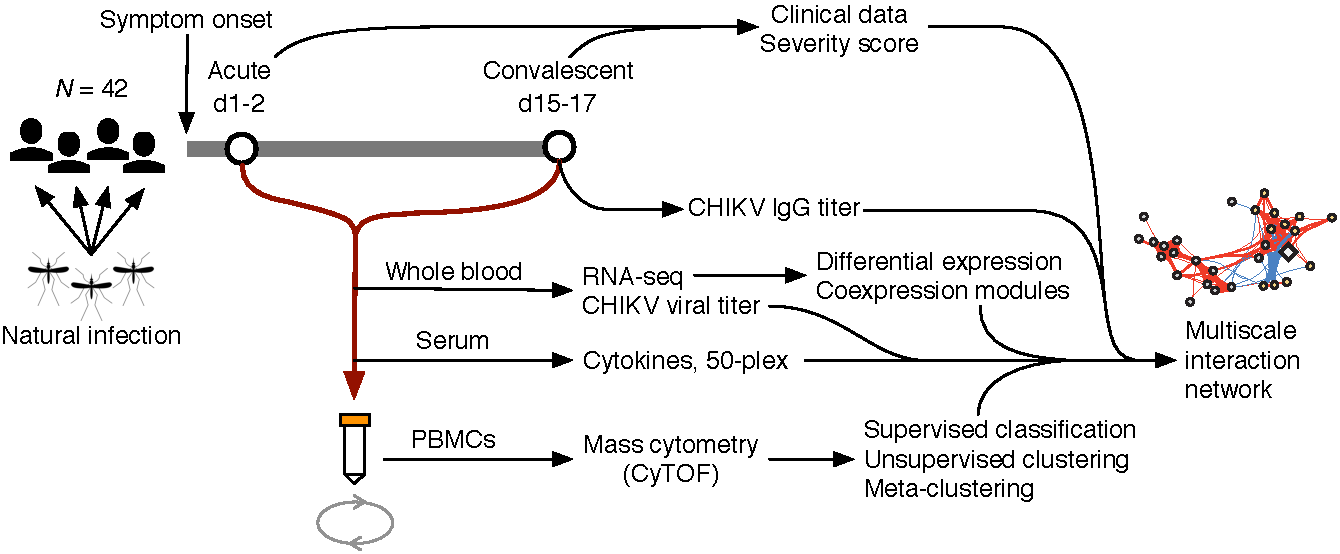
\includegraphics[width=\textwidth]{chap6/fig_1_study_design}
  \caption[Study design]{\textbf{Study design.} Blood samples were obtained from 42 pediatric cases of natural chikungunya (CHIKV) infections at an acute (d1-2) and a convalescent (d15-17) timepoint, relative to reported symptom onset. Samples were separated into whole blood, serum, and peripheral blood mononuclear cell (PBMC) aliquots for transcriptomic analysis, CHIKV viral titer assays, multiplex ELISA for cytokines, and mass cytometry (CyTOF), respectively. These data were combined with clinical data, including a severity score and a d15-17 CHIKV immunoglobulin G (IgG) titer, to create a multiscale network of interactions during the observed course of CHIKV infection.
  }
  \label{fig:chik_study_design}
\end{figure}

Sampling times closely adhered to the targeted acute (SD = 0.5d) and convalescent (SD = 0.6d) timepoints. Each blood sample was separated into aliquots of whole blood, serum, and PBMCs for transcriptomic analysis via RNA-seq, CHIKV viral titer assays, multiplex ELISA for cytokines, and mass cytometry as illustrated in Figure \ref{fig:chik_study_design}. These data were then analyzed for changes correlating with the acute and convalescent phases of infection, severe and non-severe cases, the 15d immunoglobulin G (IgG) titer, and the acute phase viral titer. The resulting signatures and clusters were combined into a multiscale interaction network capturing the global landscape of immune responses to CHIKV.

\subsection{Acute infection associates with expansion of CD14\sups{+}\allowbreak CD16\sups{+} monocytes}

\begin{figure*}[htb]
  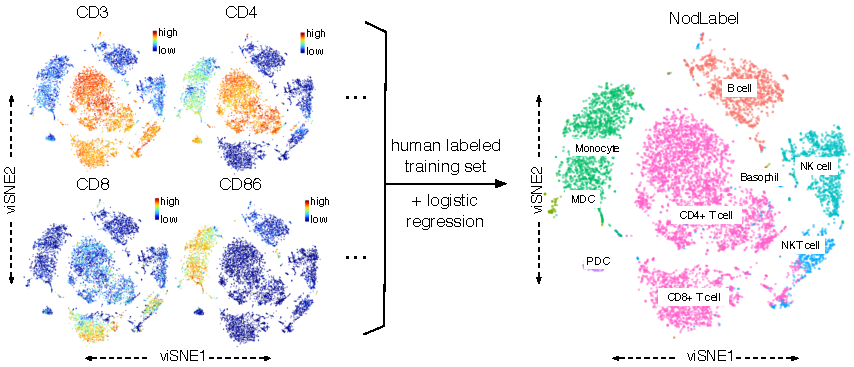
\includegraphics[width=\textwidth]{chap6/fig_2a_nodlabel_diag}
  \caption[Overview of the NodLabel procedure]{\textbf{Overview of the NodLabel procedure}, using a viSNE layout of CyTOF single-cell events. Left side, point color indicates channel values for four example channels. Right side, traditional hierarchical gating was used on a subset of samples to identify 9 major immune compartments, which was then used to train a logistic regression classifier (Nod) that applied labels for canonical leukocyte phenotypes to all samples (NodLabel).
  }
  \label{fig:nodlabel_diag}
\end{figure*}

CyTOF uses metal-labeled reagents and inductively coupled plasma mass spectrometry to overcome the limits of fluorescence spectral overlap in flow cytometry, allowing measurement of up to 50 analytes at single-cell resolution. We used CyTOF to quantify 35 immune cell surface markers (Appendix Table \ref{tab:chik_antibodies}) and the CHIKV surface protein in each of our samples. The high dimensionality of CyTOF data presents challenges for applying the traditional gating methods used in lower-dimensional flow cytometry. To address these challenges, we developed a sequential, semi-supervised approach to identify and classify immune cell populations in the CyTOF dataset. Manual gating and human-authored labels were first applied to a subset of the data to train a logistic regression classifier (called \texttt{NodLabel}) that was run on the remaining samples to broadly define 9 major immune subsets in each of the patient samples. Figure \ref{fig:nodlabel_diag} illustrates this process using a viSNE layout algorithm\autocite{Amir2013} for 2D visualizations of high-dimensional CyTOF data from a representative patient sample.

To define additional heterogeneity within each of these broad subsets, we next applied Louvain/Phenograph\autocite{Levine2015a} as an unsupervised clustering method to each \texttt{NodLabel}-identified subset in each patient sample.
\begin{figure*}[htb]
  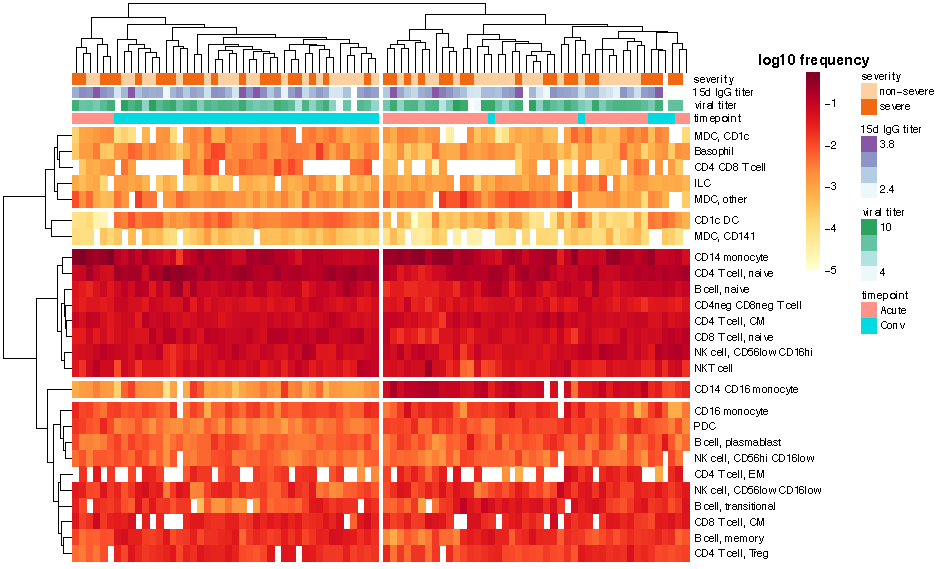
\includegraphics[width=\textwidth]{chap6/fig_2b_comm_heatmap}
  \caption[CyTOF signatures for acute CHIKV infection based on canonical immune cell phenotypes]{\textbf{CyTOF reveals signatures for acute CHIKV infection based on canonical immune cell phenotype clustering.} Heatmap of log\subs{10} scaled peripheral blood mononuclear cell (PBMC) community frequencies for all samples. Clinical variables are depicted for all samples across the top of the heatmap; 15d post symptom onset immunoglobulin G (IgG) titer and viral titer (which was measured during the acute phase) are both in units of log\subs{10} dilutions. Hierarchical clustering (using complete linkage) was applied to both samples (X axis) and communities (Y axis). Four major clusters of communities and two major clusters of samples (largely separating acute and convalescent samples) are highlighted. 
  }
  \label{fig:comm_heatmap}
\end{figure*}
While the combination of the \texttt{NodLabel} classifier and Phenograph (which we term \texttt{HybridLouvain}) is a powerful approach to define phenotypic heterogeneity in a sample, a limitation of the approach is that the identified \texttt{HybridLouvain} communities are only applicable to a single patient sample. To address this issue, we meta-clustered the individual communities across all patient samples, and meta-communities that were reproducibly identified across multiple patients were then manually annotated based on overall marker expression patterns. These annotations were then mapped back to each individual patient sample to provide consistent community definitions across all samples. Using this approach (which we term \texttt{MetaHybridLouvain}) we identified 26 communities of canonical leukocyte populations across all acute and convalescent phase samples (Figure \ref{fig:comm_heatmap}).
\begin{figure*}[htb]
  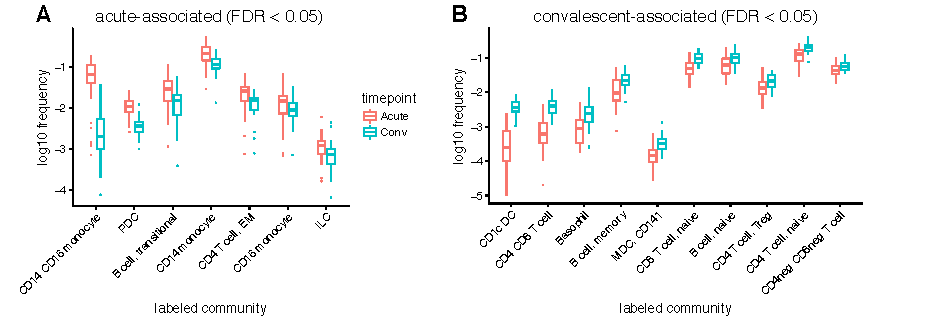
\includegraphics[width=\textwidth]{chap6/fig_2c_comm_diffs}
  \caption[PBMC communities with differing frequency across the CHIKV infection phases][-0.7cm]{\textbf{PBMC communities with differing frequency across the timepoints of CHIKV infection.} A, log\subs{10} frequencies for PBMC communities contrasted between acute and convalescent phase samples, filtered to communities where the acute phase frequency was higher at a significance threshold of FDR < 0.05 (Mann-Whitney \emph{U}). B, same as A but filtered to communities where the convalescent phase frequency was higher at a significance threshold of FDR < 0.05.
  }
  \label{fig:comm_diffs}
\end{figure*}
Hierarchical clustering by sample revealed two clusters that generally separated by timepoint, with no communities corresponding to any apparent contrasts in severity, 15d IgG titer, or acute phase viral titer (Figure \ref{fig:comm_heatmap}). Clustering by community frequency reveals a distinct contrast in CD14\sups{+}\allowbreak CD16\sups{+} monocyte frequencies between the acute and convalescent phases (vertical axis, Figure \ref{fig:comm_heatmap}). This is the most expanded population at the acute timepoint (Figure \ref{fig:comm_diffs}A), and the difference was highly significant (Bonferroni-corrected [BF] \emph{P} = 1.9e-09). Other populations also comparatively upregulated during the acute phase were plasmacytoid dendritic cells (PDCs) (BF \emph{P} = 4.7e-13) and CD14\sups{+} monocytes (BF \emph{P} = 0.0019), with four additional populations identified at a threshold false discovery rate (FDR) < 0.05 (Figure \ref{fig:comm_diffs}A). Ten populations were comparatively downregulated at the acute phase and thereby convalescent-associated at FDR < 0.05 (Figure \ref{fig:comm_diffs}B), with the strongest difference being observed in CD1c dendritic cells (DCs) (BF \emph{P} = 3.9e-19).

\subsection{Monocytes, dendritic cells, and B cells express CHIKV surface protein during acute infection}

\begin{marginfigure}
  \centering
  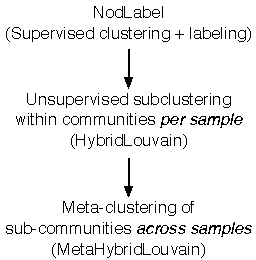
\includegraphics[width=0.7\textwidth]{chap6/fig_3a_mhl_diag}
  \vspace{1em}
  \caption[Overview of the \texttt{MetaHybridLouvain} procedure]{Overview of the \texttt{MetaHybridLouvain} procedure.}
  \label{fig:mhl_diag}
\end{marginfigure}

Classifying CyTOF events into only the canonical leukocyte populations ignores much of the richness of these data, which can reveal previously unrecognized diversity and heterogeneity within each of these populations. The advantage of our \texttt{MetaHybridLouvain} approach (Figure \ref{fig:mhl_diag}) is that it allows for unbiased identification of phenotypically heterogenous \subcommunities{} within each of the canonical immune subsets,\autocite{Samusik2016} e.g., a \subcommunity{} of CD14\sups{+} monocytes as defined by a specific, reproducible marker expression pattern across multiple samples. This allowed for the identification of up to nine \subcommunities{} within certain defined canonical immune populations (Figure \ref{fig:mhl_visne}, \ref{fig:mhl_subcomms}), producing a total of 57 \subcommunities{}. More detailed results of \texttt{MetaHybridLouvain} for the representative sample used in Figure \ref{fig:nodlabel_diag} and \ref{fig:mhl_visne} are depicted in Appendix Figures \ref{fig:mhl_example}-\ref{fig:mhl_example_cont}.

\begin{figure}[htb]
  \centering
  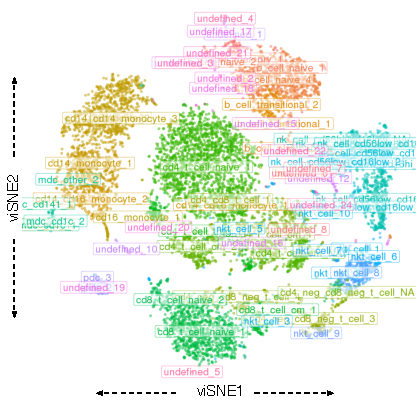
\includegraphics[width=0.8\textwidth]{chap6/fig_3b_mhl_visne}
  \caption[viSNE layout of \texttt{MetaHybridLouvain} \subcommunities{}]{viSNE layout of CyTOF single-cell events from the same representative sample as Figure \ref{fig:nodlabel_diag}, now with labels for peripheral blood mononuclear cell (PBMC) \subcommunities{} detected by \texttt{MetaHybridLouvain} drawn at the centroid of each \subcommunity{}.
  }
  \label{fig:mhl_visne}
\end{figure}
\begin{marginfigure}
  \centering
  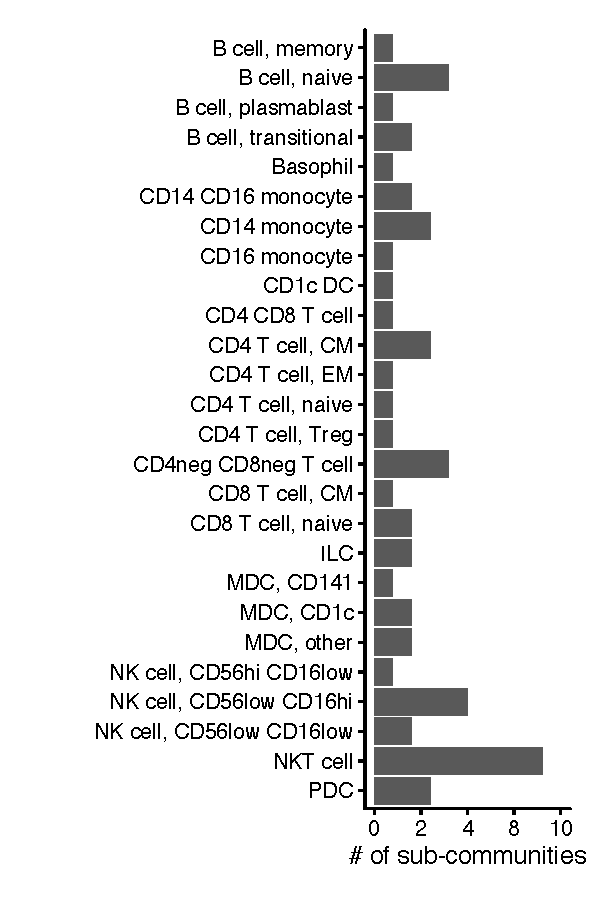
\includegraphics[width=\textwidth]{chap6/fig_3c_mhl_subcomms}
  \caption[Number of \subcommunities{} detected by \texttt{MetaHybridLouvain} per canonical phenotype]{Number of \subcommunities{} detected by \texttt{MetaHybridLouvain} for each of the canonical leukocyte phenotypes.}
  \label{fig:mhl_subcomms}
\end{marginfigure}

Having dissected the cellular heterogeneity of the samples at high resolution, we went on to identify leukocyte populations that have comparatively high levels of CHIKV surface protein during the acute phase of infection. Qualitatively, in the representative patient sample, CHIKV surface protein was expressed by distinct populations of leukocytes in the viSNE layout (Figure \ref{fig:chikv_visne})—in particular monocytes, dendritic cells, and B cells (compare with Figures \ref{fig:nodlabel_diag} and \ref{fig:mhl_visne}). Quantitatively, across all samples, monocytes and dendritic cells displayed the strongest contrasts in mean CHIKV channel values per sample between acute and convalescent timepoints (Figure \ref{fig:chikv_diffs}).
\begin{figure}[htb]
  \centering
  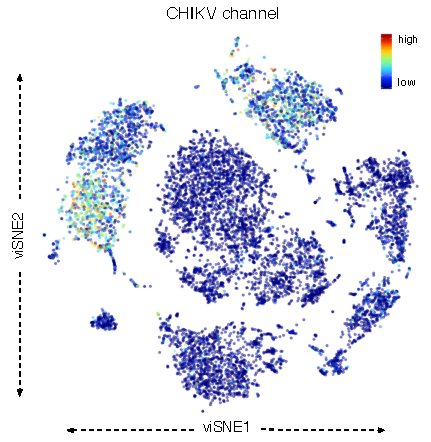
\includegraphics[width=0.8\textwidth]{chap6/fig_3d_chikv_visne}
  \caption[viSNE layout of CHIKV surface protein expression levels]{viSNE layout of CyTOF single-cell events from the same representative sample as Figure \ref{fig:nodlabel_diag} and \ref{fig:mhl_visne}, now with points colored according to the CHIKV channel. By qualitative comparison with Figure \ref{fig:nodlabel_diag} (reproduced below), monocytes, myeloid dendritic cells (MDCs), and B cells have the highest CHIKV surface protein expression. 
  }
  \label{fig:chikv_visne}
\end{figure}
CHIKV-positive cell populations largely fell along canonical leukocyte phenotype boundaries, with all three \subcommunities{} of CD14\sups{+} monocytes (BF \emph{P} = 2.5e-26, 2.7e-24, 8.1e-16), both \subcommunities{} of CD1c MDCs (BF \emph{P} = 4.2e-15 and 4.3e-08), all CD1c DCs (BF \emph{P} = 4.3e-16), and both \subcommunities{} of CD14\sups{+}\allowbreak CD16\sups{+} monocytes (BF \emph{P} = 2.5e-09 and 2.3e-06) identified as significantly more CHIKV-positive during the acute phase. Interestingly, although the differences were less pronounced, three \subcommunities{} of B cells were also observed to express significantly higher CHIKV surface protein during acute infection: the only community of memory B cells (BF \emph{P} = 3.2e-09) and two of the four \subcommunities{} of naïve B cells (BF \emph{P} = 9.7e-06 and 0.00022). Although CHIKV surface protein expression only correlates with (and does not establish) tropism of the virus, our data suggest that among PBMCs, CHIKV preferentially infects monocytes and dendritic cells, while displaying lower but substantial affinity for B cells.

\begin{marginfigure}[-17cm]
  \centering
  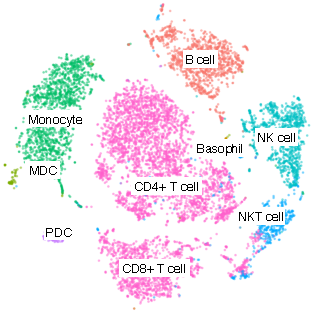
\includegraphics[width=\textwidth]{chap6/fig_2a-repeat_nodlabel_just_visne}
\end{marginfigure}

\begin{marginfigure}[-5cm]
  \centering
  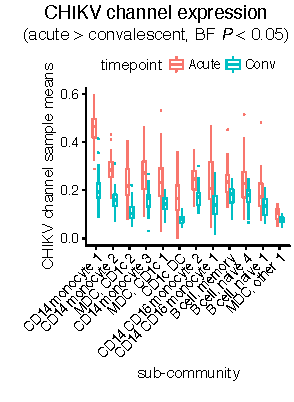
\includegraphics[width=\textwidth]{chap6/fig_3e_chikv_diffs}
  \caption[Number of \subcommunities{} detected by \texttt{MetaHybridLouvain} per canonical phenotype]{Differences in CHIKV surface protein expression between acute phase and convalescent phase samples per \texttt{MetaHybridLouvain} \subcommunity. \Subcommunities{} are ordered by largest to smallest difference and filtered to \subcommunities{} where the median of the channel means per sample was higher in the acute phase samples at a significance threshold of Bonferroni \emph{P} < 0.05. \Subcommunities{} are named by their parent canonical community name plus an arbitrary number, up to the counts given in Figure \ref{fig:mhl_subcomms}.}
  \label{fig:chikv_diffs}
\end{marginfigure}

\subsection{CD14\sups{+} and CD14\sups{+}\allowbreak CD16\sups{+} monocyte \subcommunities{} exhibit contrasting behaviors during acute infection}

\begin{figure*}[p]
  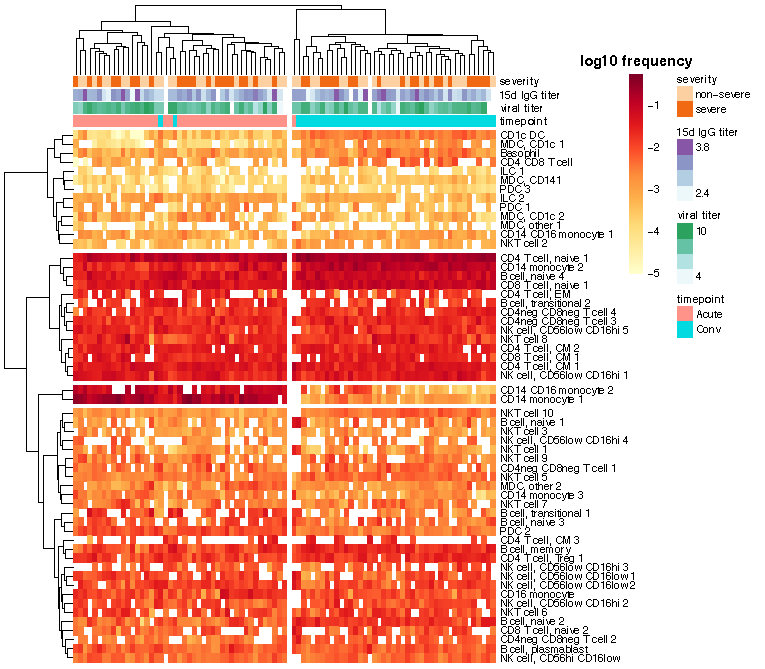
\includegraphics[width=\textwidth]{chap6/fig_3f_mhl_subcomm_heatmap}
  \fullwidthlabelcaption{fig:subcomm_heatmap}{Specific monocyte \subcommunities{} undergo expansion during acute CHIKV infection}{
  \textbf{Specific monocyte \subcommunities{} undergo expansion during acute CHIKV infection.} Heatmap of log\subs{10} scaled PBMC \subcommunity{} frequencies for all samples. Clinical variables are depicted for all samples across the top of the heatmap; 15d post symptom onset immunoglobulin G (IgG) titer and viral titer (which was measured during the acute phase) are both in units of log\subs{10} dilutions. Hierarchical clustering (using complete linkage) was applied to both samples (X axis) and \subcommunities{} (Y axis). Four major clusters of \subcommunities{} and two major clusters of samples (largely separating acute and convalescent samples) are highlighted. 
  }
\end{figure*}

Although CD14\sups{+}\allowbreak CD16\sups{+} monocytes expand during the acute phase of infection, community subclustering provides more detail on particular \subcommunities{} that associate with the acute phase. Hierarchical clustering of samples by \subcommunity{} frequencies separates the samples by timepoint more effectively than canonical population frequencies alone (Figure \ref{fig:subcomm_heatmap}, compare with Figure \ref{fig:comm_heatmap}), with only 3/88 (3\%) of samples misclassified between the two major clusters. Again, however, there was no apparent clustering of samples that corresponded to contrasts in clinical severity, 15d IgG titer, or acute phase viral titer. Stratifying by the acute and the convalescent phases, there were no significant differences
\begin{figure}[tb]
  \centering
  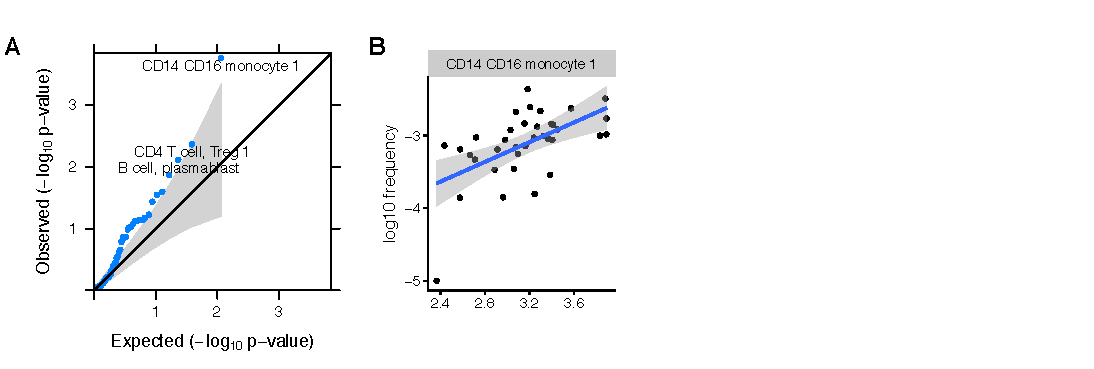
\includegraphics[width=0.88\textwidth]{chap6/fig_S2_corr_IgG_cd14cd16_mono_1}
  \caption[Correlations between acute phase cell \subcommunity{} frequencies and 15d CHIKV IgG titer]{
  \textbf{Correlations between acute phase cell \subcommunity{} frequencies and log\subs{10} CHIKV IgG titer at 15d post-symptom onset.} A, Q-Q plot of the distribution of observed –log\subs{10} \emph{P} values against the distribution of –log\subs{10} \emph{P} values expected under the null hypothesis (that Spearman’s $\rho = 0$ for all \subcommunities). Gray shaded band indicates the 95\% confidence interval for the expected \emph{P} value distribution under the null hypothesis. B, Scatterplots of log\subs{10} cell \subcommunity{} frequencies against log\subs{10} IgG CHIKV titer at the 15d timepoint for the CD14\sups{+}CD16\sups{+} monocyte 1 correlation, which is the only correlation significant after multiple hypothesis correction (BF \emph{P} = 0.0097, Spearman’s $\rho$ = 0.60).
  }
  \label{fig:corr_cytof_igg}
\end{figure}
in any \subcommunity{} frequencies between severe and non-severe cases at FDR < 0.1. Within either timepoint, there were also no significant correlations between \subcommunity{} frequencies and log-transformed acute phase viral titers at FDR < 0.1. There was, however, a single significant correlation between CD14\sups{+}\allowbreak CD16\sups{+} monocyte \subcommunity{} 1 at the acute phase and the 15d (convalescent) IgG titer
\begin{figure*}[htb]
  \centering
  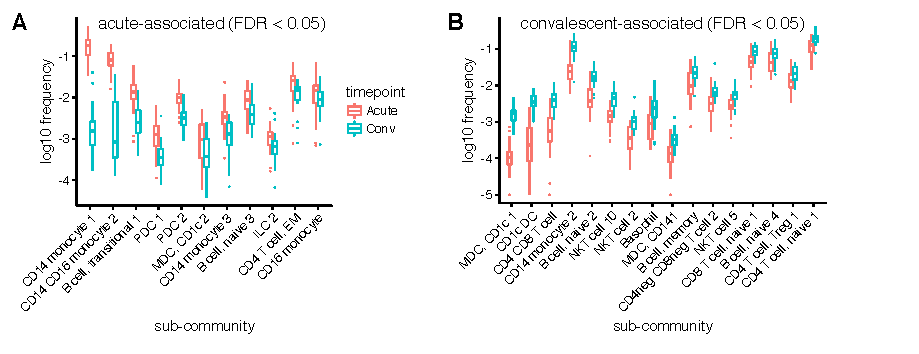
\includegraphics[width=0.95\textwidth]{chap6/fig_3g_subcomm_diffs}
  \caption[PBMC \subcommunities{} with differing frequency across the CHIKV infection phases]{
  \textbf{PBMC \subcommunities{} with differing frequency across the timepoints of CHIKV infection.} A, log\subs{10} frequencies for PBMC \subcommunities{} contrasted between acute and convalescent phase samples, filtered to \subcommunities{} where the acute phase frequency was higher at a significance threshold of FDR < 0.05 (Mann-Whitney \emph{U}). B, same as A but filtered to \subcommunities{} where the convalescent phase frequency was higher at a significance threshold of FDR < 0.05.
  }
  \label{fig:subcomm_diffs}
\end{figure*}
(BF \emph{P} = 0.0097, Spearman’s $\rho$ = 0.60; see Figure \ref{fig:corr_cytof_igg}), with no significant correlations among convalescent \subcommunity{} frequencies at FDR < 0.1.

Among \subcommunities{} significantly expanded during the acute phase, two particular expansions separated from the others by an order of magnitude (Figure \ref{fig:subcomm_diffs}A), specifically \subcommunity{} 1 of CD14\sups{+} monocytes (BF \emph{P} = 7.7e-21) and \subcommunity{} 2 of CD14\sups{+}\allowbreak CD16\sups{+} monocytes (BF \emph{P} = 2.8e-15).
\begin{figure*}[htb]
  \centering
  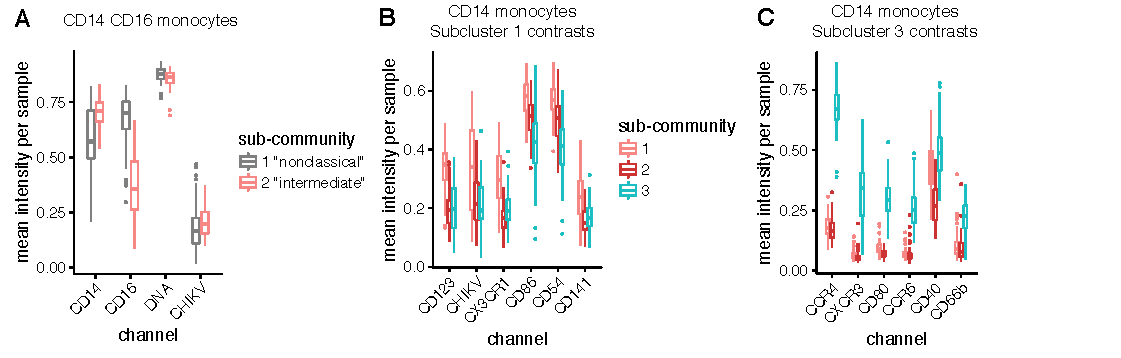
\includegraphics[width=0.95\textwidth]{chap6/fig_4_monocyte_subpops}
  \caption[Marker expression differences between sub-communities of CD14\sups{+}CD16\sups{+} monocytes and CD14\sups{+} monocytes]{
  \textbf{Marker expression differences between sub-communities of CD14\sups{+}CD16\sups{+} monocytes and CD14\sups{+} monocytes}, depicted as boxplots of the mean expression levels for all samples. A, relative expression of CD14\sups{+} and CD16\sups{+} in CD14\sups{+}CD16\sups{+} sub-communities indicates that sub-community 1 is a CD14\sups{+}CD16\sups{++} (aka “non-classical”) phenotype, while sub-community 2 is a CD14\sups{++}CD16\sups{+} (aka “intermediate”) phenotype. Differences shown here are significant at FDR < 0.05; for a view of all differences significant at this threshold, see Appendix Figure \ref{fig:cd14cd16_channel_diffs}. B, relative expression of six markers that most differentiate (by the difference in medians) sub-community 1 of CD14\sups{+} monocytes from the other sub-communities. C, relative expression of six markers that most differentiate (by the difference in medians) sub-community 3 of CD14\sups{+} monocytes from the other sub-communities. Note: Channels shown in B and C are a subset of the differences that are significant at FDR < 0.05; for a view of all differences significant at FDR < 0.05 see Appendix Figure \ref{fig:cd14_channel_diffs}.
  }
  \label{fig:subcomm_marker_diffs}
\end{figure*}
When examining the other two \subcommunities{} of CD14\sups{+} monocytes, one is also expanded during the acute phase but to a lesser extent (\subcommunity{} 3, BF \emph{P} = 5.6e-06) while the other instead is expanded during the convalescent phase (\subcommunity{} 2, BF \emph{P} = 1.6e-10). At FDR < 0.1, \subcommunity{} 1 of CD14\sups{+}\allowbreak CD16\sups{+} monocytes, which is the only other \subcommunity{} of CD14\sups{+}\allowbreak CD16\sups{+} monocytes, is not significantly different across timepoints. Other \subcommunities{} associating with the convalescent phase at FDR < 0.05 include MDCs, CD1c DCs, B cells, T cells, and basophils (Figure \ref{fig:subcomm_diffs}B).

Since different \subcommunities{} of CD14\sups{+}\allowbreak CD16\sups{+} and CD14\sups{+} monocytes displayed distinctive responses to acute CHIKV infection, we looked for marker differences that could better define these \subcommunities{}. Examination of the two CD14\sups{+}\allowbreak CD16\sups{+} monocyte \subcommunities{} (Figure \ref{fig:subcomm_marker_diffs}A) revealed that among all significant marker differences, \subcommunity{} 1 had higher CD16 expression (BF \emph{P} = 5.7e-19) and \subcommunity{} 2 had higher CD14 expression (BF \emph{P} = 6.4e-05). This corresponded to \subcommunities{} commonly called “nonclassical” CD14\sups{+}\allowbreak CD16\sups{++} and “intermediate” CD14\sups{++}\allowbreak CD16\sups{+} monocytes,\autocite{Wong2011,Ziegler-Heitbrock2010} implying that in our study, “intermediate” monocytes were substantially expanded during acute CHIK infection while “nonclassical” monocytes were unchanged. Significant contrasts in the expression of many other surface markers at FDR < 0.05 (Appendix Figure \ref{fig:cd14cd16_channel_diffs}) and the consistent identification of these patterns across the majority of samples (Appendix Figures \ref{fig:cd14cd16_subcomm_1_heatmap}-\ref{fig:cd14cd16_subcomm_2_heatmap}) confirmed the distinction between these \subcommunities{}.

Among the three \subcommunities{} of CD14\sups{+} monocytes, we discovered two that were associated with acute infection, including one with a previously unreported phenotype. \subcommunity{} 1 (the \subcommunity{} most strongly associated with acute infection and also expressing the highest levels of CHIKV surface protein) was characterized by having relatively higher levels of CD123, CX3CR1, CD86 and CD54 expression (Fig \ref{fig:subcomm_marker_diffs}B), generally consistent with a more activated phenotype relative to \subcommunity{} 2, which was more prevalent during convalescence. Monocyte \subcommunity{} 3 was also expanded during acute infection, though at a much lower frequency than monocyte \subcommunity{} 1, and displayed similar levels of CD40, consistent with an activated phenotype. Interestingly, however, this subset also exhibited comparatively high expression of markers that are not classically associated with monocytes, particularly the chemokine receptor CCR4, as well as CXCR3 and CCR6 (Figure \ref{fig:subcomm_marker_diffs}C). We further confirmed that this \subcommunity{} did not express canonical markers associated with other major cell types, such as T cells or B cells, to verify that it did not represent an artifact of cell-cell doublets. Again, significant contrasts in the expression of many surface markers at FDR < 0.05 (Kruskal-Wallis test, Appendix Figure \ref{fig:cd14_channel_diffs}), and a consistent pattern for the phenotype identified across the majority of samples (Appendix Figures \ref{fig:cd14_subcomm_1_heatmap}-\ref{fig:cd14_subcomm_3_heatmap}) confirmed the distinction between these \subcommunities{}. Given the strongly contrasting associations of these \subcommunities{} with the phase of infection, these data suggest that unappreciated heterogenity within CD14\sups{+} monocyte phenotypes may enable different roles for \subcommunities{} of these monocytes during CHIKV infection.  

\subsection{Monocyte-associated cytokine concentrations increase during acute infection}

\begin{figure*}[htb]
  \centering
  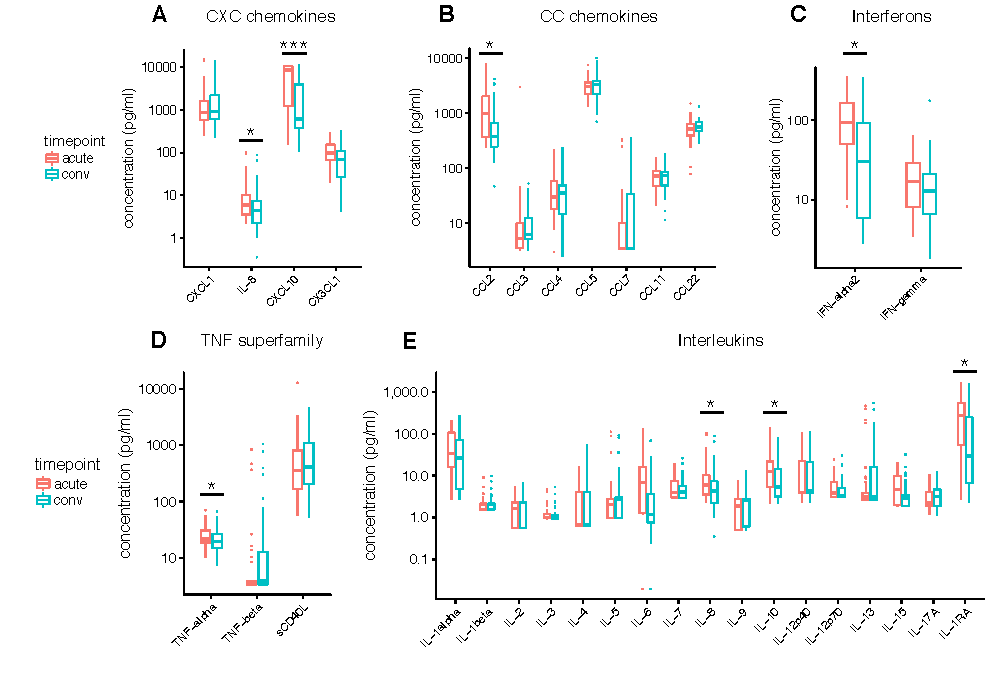
\includegraphics[width=\textwidth]{chap6/fig_5_luminex}
  \caption[Differences in serum cytokine and chemokine levels between the acute and convalescent phase samples]{
  \textbf{Differences in serum cytokine and chemokine levels between the acute and convalescent phase samples.} Wilcoxon signed-rank test was used to determine statistical significance, with a Benjamini-Hochberg adjustment for FDR (n = 41). *\emph{P} < 0.05, ***\emph{P} < 0.001. A, CXC chemokines. B, CC chemokines. C, interferons. D, TNF superfamily cytokines. E, interleukins. Note that IL-8 is both a CXC chemokine (CXCL8) and an interleukin, so it is depicted twice. Growth factors and colony-stimulating factors are shown in Appendix Figure \ref{fig:nonsig_luminex}.
  }
  \label{fig:luminex}
\end{figure*}

To profile the effect of CHIKV on circulatory markers for inflammation and immune signaling, we used a multiplexed microbead immunoassay (Luminex) to measure serum concentrations of 41 cytokines, chemokines, and growth factors in all 84 samples. In our study, seven cytokines were significantly different (Wilcoxon signed-rank test with Benjamini-Hochberg adjustment) across acute and convalescent timepoints at FDR < 0.05 (Figure \ref{fig:luminex}A-E). The strongest contrast was the IFN-γ inducible, monocyte-secreted chemokine CXCL10 (BF \emph{P} = 0.00085). Significant increases (FDR < 0.05) were also observed for IL-10 (a monocyte-secreted anti-inflammatory cytokine), CCL2 (monocyte chemoattractant protein 1), IFN-α2, TNF-α, IL-8, and IL-1RA. There were no significant differences observed among growth factors or colony-stimulating factors (Appendix Figure \ref{fig:nonsig_luminex}). No analyte concentrations were significantly decreased during acute infection.

To determine if cytokine levels could be associated with changes in specific cell \subcommunities{}, we correlated log-scaled Luminex analyte concentrations with log-scaled \subcommunity{} frequencies (using Pearson’s \emph{r}). Hierarchical clustering revealed that cytokine and growth factors concentrations tended to correlate with each other rather than with any of the subpopulation frequencies (Appendix Figure \ref{fig:corrplot_luminex_cytof_bothtimes}). This remained unchanged when stratifying into acute phase (Appendix Figure \ref{fig:corrplot_luminex_cytof_acute}) or convalescent phase (Appendix Figure \ref{fig:corrplot_luminex_cytof_conv}) samples, with the only exception being a cluster containing CXCL1, sCD40L, PDGF-AA, and PDGF-AB/BB that consistently separated from one major cluster containing all other Luminex analytes. Since the most pronounced expansions during the acute phase involved monocyte subpopulations, we then performed a more focused analysis on correlations between all cytokines and monocyte subpopulations, stratifying by timepoint to capture potential regulatory relationships rather than the primary contrast of the study. Within acute phase samples, cytokines generally had varied correlations with each of the monocyte subpopulations, but at the convalescent timepoint, the monocyte chemoattractant CCL2 clustered separately from all other cytokines and had positive correlations with all monocyte subpopulations (Figure \ref{fig:luminex_monocyte_corr}, BF \emph{P} = 0.0021). This is suggestive of a relatively important regulatory role for CCL2 on monocyte populations during the convalescent phase of infection.

\begin{figure*}[hb]
  \centering
  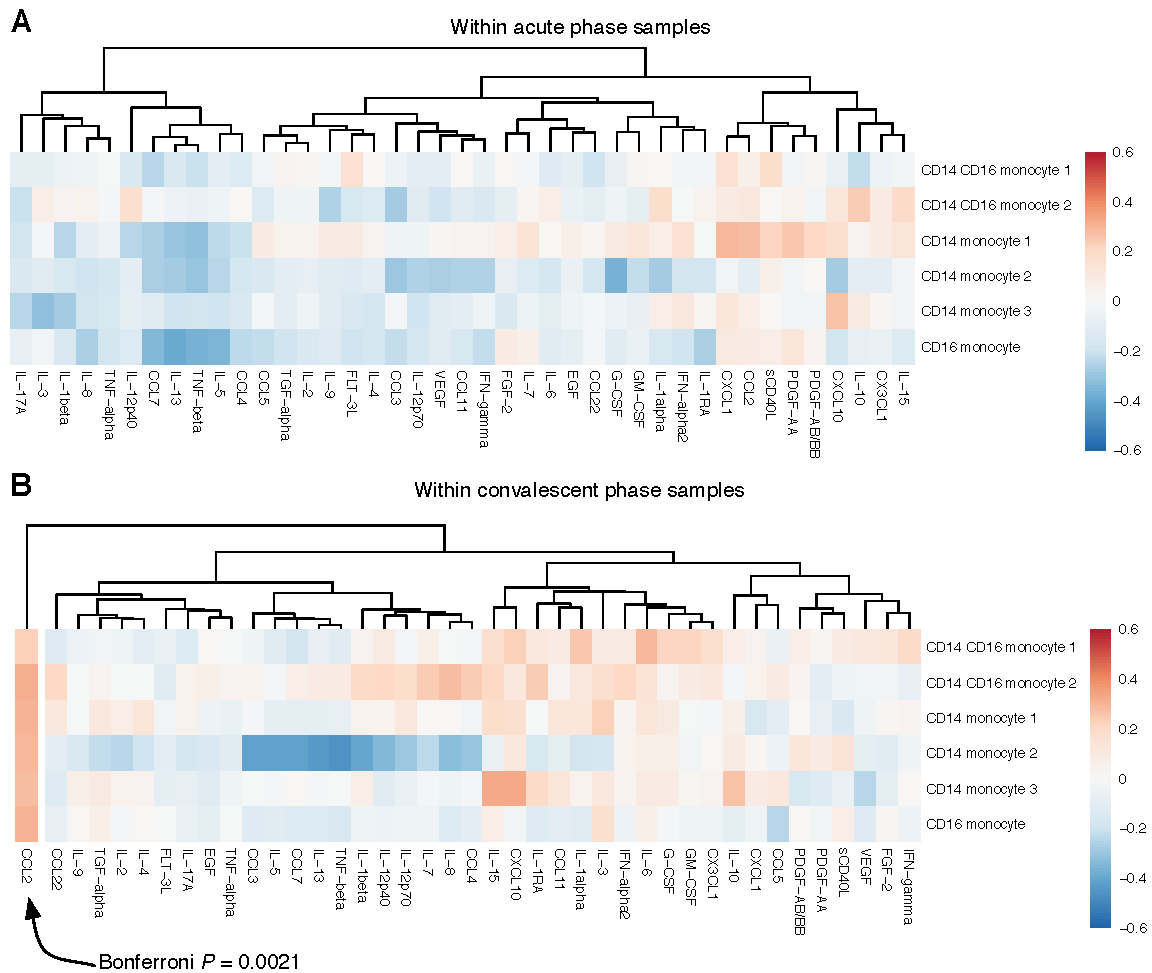
\includegraphics[width=\textwidth]{chap6/fig_S14_corrplots_cytokines_monocytes.pdf}
  \caption[Clustered heatmap of Pearson correlations between log-scaled serum cytokine concentration and log-scaled monocyte subphenotype frequencies]{
  \textbf{Clustered heatmap of Pearson correlations between log-scaled serum cytokine concentration and log-scaled monocyte subphenotype frequencies.} A, within acute phase samples. B, within convalescent phase samples.
  }
  \label{fig:luminex_monocyte_corr}
  \setfloatalignment{b}
\end{figure*}

\subsection{Acute infection associates with upregulated transcription of monocyte-associated cytokine genes}

To capture global transcriptional changes during CHIKV infection, polyadenylated RNA from whole blood was analyzed by RNA-seq for all 42 patients at both sampled timepoints with two technical replicates per sample. A Tuxedo pipeline was used for read alignment, quantification and differential expression analysis of genes. Since previous studies of gene and protein changes during acute CHIKV infection targeted cytokines, chemokines, and innate immunity mechanisms,\autocite{Chow2011,Hoarau2010,Ng2009,Teng2015,Wauquier2011} we first present results for differentially expressed genes in these pathways for comparison with our Luminex data and the literature, before moving to a global analysis in the subsequent section.

Appendix Figure \ref{fig:corrplot_luminex_mrna_both} shows that across the two timepoints, log-scaled serum concentrations for the significantly CHIK-upregulated cytokines (as measured by Luminex, Figure \ref{fig:luminex}) did not correlate with whole blood gene expression for corresponding genes, using log-scaled units of fragments per kilobase of exon per million reads mapped (FPKM). Since this could be due to different “baseline” serum cytokine or cytokine gene expression levels, we repeated the analysis with all acute phase measurements normalized against the convalescent phase measurements, but clustering did not change (Appendix Figure \ref{fig:corrplot_luminex_mrna_normacuteconv}). This suggests that the regulation of serum cytokine levels is not primarily driven by transcriptional changes in leukocytes, but could involve substantial expression from other tissues and secretory and protein-level regulatory processes. Alternatively, the technical variance of the Luminex assay for our samples may simply have been too high to draw out meaningful correlations with gene expression. 

\begin{sidewaysfigure}[hp]
  \sidewaysvspace
  \centering
  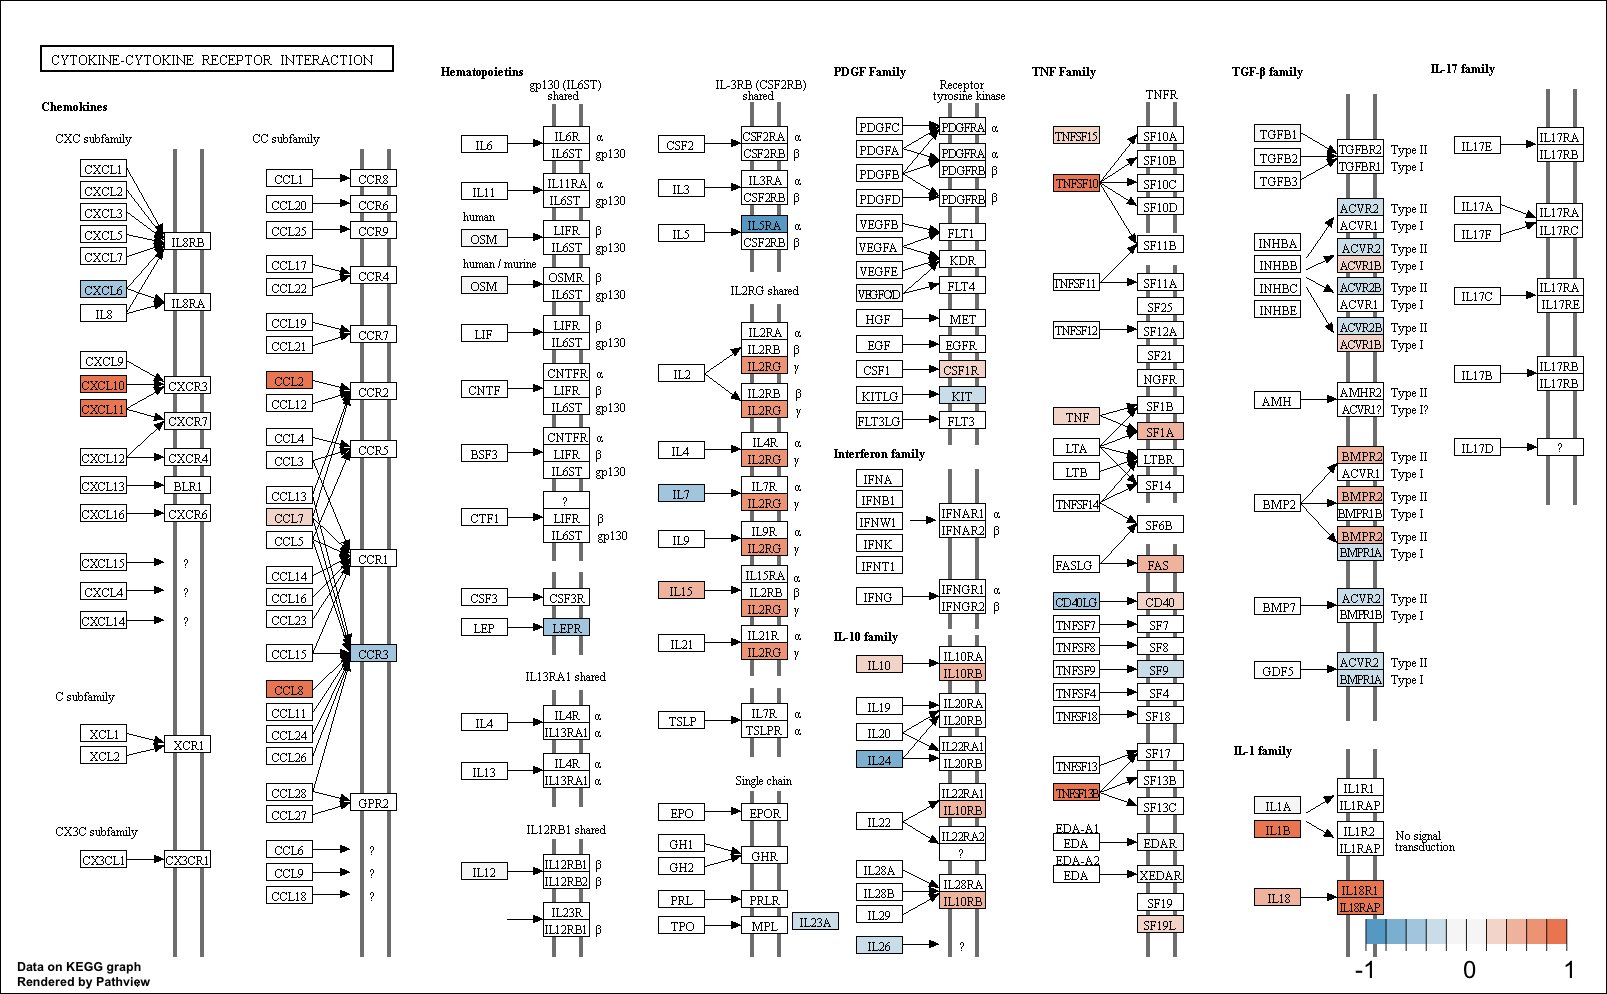
\includegraphics[width=\textwidth]{chap6/fig_S17_hsa04060.timepoint.log2fc.png}
  \fullwidthlabelcaption{fig:pathview_hsa04060}{Pathview plot of log\subs{2} fold change in expression of cytokine and receptor genes}{
  \textbf{Pathview plot of log\subs{2} fold change in gene expression between acute and convalescent timepoints for the cytokine-cytokine receptor interaction pathway}, using KEGG annotations (accession \href{http://www.genome.jp/dbget-bin/www\textunderscore bget?hsa04060}{hsa04060}). Positive values indicate upregulation during the acute phase of infection.
  }
\end{sidewaysfigure}

Differential expression of all genes was quantified by log\subs{2} fold change (log2FC) in units of FPKM and considered significant at an FDR threshold of <0.05. Among CXC and CC subfamily chemokines, we observed transcriptional upregulation of \emph{CXCL10}, \emph{CXCL11}, \emph{CCL2}, \emph{CCL7}, and \emph{CCL8} (Figure \ref{fig:pathview_hsa04060}). Of these, monocyte-secreted \emph{CXCL10} and monocyte chemoattractant \emph{CCL2} concur with the changes in serum cytokine concentrations described above (Figure \ref{fig:luminex}A-B), and \emph{CCL8} (whose gene product was not measured with Luminex) is notable for being another monocyte chemoattractant (MCP-2). Interestingly, although serum IFN-α levels were significantly elevated during acute infection (Figure \ref{fig:luminex}C), none of the interferon family genes were differentially expressed (Figure \ref{fig:pathview_hsa04060}). Upregulation of the \emph{TNF} gene is concordant with the significant increase in serum TNF-α concentration (Figures \ref{fig:pathview_hsa04060} and \ref{fig:luminex}D), and other significantly upregulated TNF superfamily genes included \emph{TNFSF15}, \emph{TNFSF10}, and \emph{TNFSF13B} (Figure \ref{fig:pathview_hsa04060}). While upregulation of \emph{IL10} gene expression was concordant with the serum cytokine measurements, in contrast to those data, we did not observe differential expression of \emph{IL8} (Figures \ref{fig:pathview_hsa04060} and \ref{fig:luminex}E). 

We also examined differential expression of genes during acute infection for known components of innate immunity pathways annotated in KEGG\autocite{Ogata1999} (Appendix Figures \ref{fig:pathview_hsa04062}-\ref{fig:pathview_hsa05164}). Of these pathways, JAK-STAT signaling genes were significantly transcriptionally upregulated, with smaller but significant upregulation of NF-κB genes (Appendix Figures \ref{fig:pathview_hsa04062} and \ref{fig:pathview_hsa04630}). Among toll-like receptor (TLR) genes, \emph{TLR5} and \emph{TLR3} (whose gene product is a dsRNA receptor) were significantly upregulated (Appendix Figure \ref{fig:pathview_hsa04620}). Both \emph{RIG-I} and \emph{MDA5}, which are cellular sensors for viral RNA, were significantly upregulated (Appendix Figure \ref{fig:pathview_hsa04622}). Of the TNF superfamily receptors, \emph{TNFR1} was upregulated but \emph{TNFR2} was not (Appendix Figure \ref{fig:pathview_hsa04668}). Of the interferon regulatory factor (IRF) genes annotated in KEGG, expression of \emph{IRF7} and \emph{IRF9} were significantly upregulated, and interestingly, all downstream transcriptional targets of IRF9 annotated in KEGG (\emph{MX1}, OAS genes, \emph{ADAR}, and \emph{PML}) were consistently upregulated during acute infection (Appendix Figure \ref{fig:pathview_hsa05164}). (Fold change values for all quantified genes and \emph{q} values are provided in Table S1.) In general, our observed modulations of human innate immunity pathways were comparable to differentially expressed genes reported for a mouse model in a recent study\sidecite[-7.2cm]{Wilson2017} (see Discussion). 

\subsection{Transcriptomic signatures for acute infection, severity, viral titer, and immunogenicity}

RNA-seq enables the estimation of transcript abundances and transcript-level differential expression analyses that may offer insights not available from gene-level quantification.\sidecite[-9.5cm]{Anders2012,Trapnell2013} We performed pseudoalignment-based quantification of transcript abundances in units of transcripts per million (TPM), followed by differential expression analysis.
\begin{marginfigure}[-7.5cm]
  \centering
  \includegraphics[width=\textwidth]{chap6/fig_6a_DET_timepoint_volcano}
  \caption[Volcano plot of differentially expressed host transcripts between acute and convalescent phase samples]{
  \textbf{Volcano plot of differentially expressed host transcripts between acute and convalescent phase samples}, with negative log\subs{10} scaled \emph{q} values (Benjamini-Hochberg adjusted \emph{P} values) on the Y axis, and the modeled $\beta$ coefficient for each transcript (corresponding to natural log transformed effect sizes) on the X axis. Transcripts to the right of the vertical dashed line were comparatively upregulated in acute phase samples, while transcripts to the left were upregulated during the convalescent phase. Transcripts that pass FDR < 0.05 are colored red. Top transcripts by \emph{q} value are individually labeled by their corresponding gene symbol. 
  }
  \label{fig:DET_timepoint_volcano}
\end{marginfigure}
\begin{figure*}[hp]
  \centering
  \includegraphics[width=0.85\textwidth]{chap6/fig_6b_DET_timepoint_heatmap}
  \fullwidthlabelcaption{fig:DET_timepoint_heatmap}{Top 50 differentially expressed host transcripts for CHIKV infection phase}{
  \textbf{Top 50 differentially expressed host transcripts for CHIKV infection phase.} Heatmap of expression measured in log\subs{10} scaled 1 + transcripts per million (TPM) for top 50 differentially expressed transcripts between acute and convalescent phase samples (2 technical replicates per patient sample). Clinical variables are depicted for all samples across the top of the heatmap; 15d post symptom onset immunoglobulin G (IgG) titer and viral titer (which was measured during the acute phase) are both in units of log\subs{10} dilutions. Hierarchical clustering (using complete linkage) was applied to both samples (X axis) and transcripts (Y axis). Two major clusters of samples (largely separating acute and convalescent samples) are highlighted.
  }
\end{figure*}
After adjusting for age and gender covariates, a strong transcriptional signature for timepoint (acute vs.\ convalescent) emerged (Figure \ref{fig:DET_timepoint_volcano}), with 28,015 transcripts differentially expressed at FDR < 0.05. The top differentially expressed transcripts (DETs), ordered by \emph{P} value, were products of the \emph{SPATS2L}, \emph{IL1RN}, \emph{EIF4B}, \emph{ABCA1}, \emph{XAF1}, and \emph{CASP1P2} genes. Hierarchical clustering of the samples by quantification of the top 50 differentially expressed transcripts readily separated samples by timepoint, with only 8/160 (5\%) of samples misclassified between the two major clusters (Figure \ref{fig:DET_timepoint_heatmap}). All paired technical replicates clustered together. The top 50 DETs notably contained many interferon-induced (IFI prefix) gene products that cluster along the vertical axis (Figure \ref{fig:DET_timepoint_heatmap}).

\begin{marginfigure}[-3cm]
  \centering
  \includegraphics[width=\textwidth]{chap6/fig_6c_DET_viral_volcano}
  \caption[Volcano plot of differentially expressed host transcripts for viremic load]{
  \textbf{Volcano plot} as in Figure \ref{fig:DET_timepoint_volcano} but for DETs between samples with higher and lower CHIKV viral titer. Transcripts to the right of the vertical dashed line associated with higher viral titer, while transcripts to the left associated with lower viral titer. 
  }
  \label{fig:DET_viral_volcano}
\end{marginfigure}

Adding the log-scaled acute phase CHIK viral titer as a variable to the model of transcript expression produced a separate and substantial signature for transcription correlating with viral titer (Figure \ref{fig:DET_viral_volcano}), with 3,326 DETs at FDR < 0.05. In Figure \ref{fig:DET_viral_volcano}, an increase in transcription corresponding to higher viral titers were modeled as a positive fixed effect coefficient $\beta$. Top DETs for viral titer (by \emph{P} value) were products of the \emph{PPT1}, \emph{DDX52}, \emph{LILRB3}, \emph{CDS2}, and \emph{FBXO7} genes, with all but the last upregulated in cases with higher viremia.

We assessed the composition of these two large signatures with standard gene set enrichment analyses for functional annotation libraries. The top 1,000 genes in the timepoint DET signature were most significantly enriched for gene ontology (GO), Panther, and Reactome annotations related to defense against viral infection, TLR signaling, and interferon signaling (Table \ref{tab:chik_det_enrichr}). The top 1,000 genes in the viral titer DET signature were most significantly enriched for terms related to leukocyte activation, chemokine and cytokine signaling, and interferon signaling (Table \ref{tab:chik_det_enrichr}). These enrichments suggest that the timepoint of infection sensibly corresponds to a maximal contrast in transcription of innate antiviral immunity genes, while the level of viremia correlates with increased transcription of immune cell activation and recruitment signals.

\begin{marginfigure}[-9.5cm]
  \centering
  \includegraphics[width=\textwidth]{chap6/fig_6d_DET_severity_volcano}
  \caption[Volcano plot of differentially expressed host transcripts for symptom severity]{
  \textbf{Volcano plot} as in Figure \ref{fig:DET_timepoint_volcano} but for DETs between patients with more severe and less severe acute phase symptoms. Transcripts to the right of the vertical dashed line were comparatively upregulated in severe cases, while transcripts to the left were upregulated in non-severe cases. 
  }
  \label{fig:DET_severity_volcano}
\end{marginfigure}
\begin{marginfigure}[-1cm]
  \centering
  \includegraphics[width=0.8\textwidth]{chap6/fig_S24_sleuth-wt-severity-qq}
  \caption[Q-Q plot of the distribution of observed –log\subs{10} \emph{P} values for severity DETs against the distribution expected under the null hypothesis]{
    \textbf{Q-Q plot of the distribution of observed –log\subs{10} \emph{P} values for severity DETs against the distribution expected under the null hypothesis.} Gray shaded band indicates the 95\% confidence interval for the null distribution.
  }
  \label{fig:DET_severity_qq}
\end{marginfigure}
\begin{table*}[htb]
  \centering
\footnotesize
\begin{tabular}{P{0.85in} P{0.75in} P{1.65in} l l l P{0.7in}}
  \toprule
  Gene set$^a$ (\#~genes) & Annotation set & Term & Overlap & \emph{q} value$^b$ & \emph{Z}-score & Combined score$^c$ \\
  \midrule
  \multirow{9}{0.85in}{Top 1000 DETs for timepoint: acute vs. convalescent (593)}
   & \multirow{3}{0.75in}{GO Biological Process 2015} & defense response to virus  & 40/147 & 5.98e-24 & -2.26 & 120 \\
     \cmidrule{3-7}
   &  & response to virus  & 47/250 & 1.50e-21 & -2.37 & 114 \\
     \cmidrule{3-7}
   &  & viral life cycle  & 36/118 & 1.51e-23 & -2.14 & 112 \\
   \cmidrule{2-7}
   & \multirow{3}{0.75in}{Panther 2016} & toll receptor signaling pathway & 7/49 & 0.0425 & -1.51 & 4.76 \\
     \cmidrule{3-7}
   &  & apoptosis signaling pathway & 8/102 & 0.191 & -1.39 & 2.30 \\
     \cmidrule{3-7}
   &  & oxidative stress response & 4/24 & 0.190 & -1.31 & 2.18 \\
   \cmidrule{2-7}
   & \multirow{3}{0.75in}{Reactome 2016} & interferon signaling & 45/196 & 2.41e-24 & -2.10 & 114 \\
     \cmidrule{3-7}
   &  & eukaryotic translation elongation & 32/89 & 7.89e-24 & -2.01 & 107 \\
     \cmidrule{3-7}
   &  & L13a-mediated translational silencing of ceruloplasmin expression & 34/106 & 7.89e-24 & -1.95 & 103 \\
  \cmidrule{1-7}
  \multirow{9}{0.85in}{Top 1000 DETs for viral titer (874)}
   & \multirow{3}{0.75in}{GO Biological Process 2015} & leukocyte activation  & 47/373 & 2.50e-07 & -2.38 & 36.2 \\
     \cmidrule{3-7}
   &  & cellular response to cytokine stimulus  & 50/471 & 8.20e-06 & -2.46 & 28.8 \\
     \cmidrule{3-7}
   &  & cytokine-mediated signaling pathway & 41/342 & 8.20e-06 & -2.39 & 28.0 \\
   \cmidrule{2-7}
   & \multirow{3}{0.75in}{Panther 2016} & Inflammation mediated by chemokine and cytokine signaling pathway & 23/188 & 0.000695 & -1.83 & 13.3 \\
     \cmidrule{3-7}
   &  & CCKR signaling map & 17/165 & 0.0346 & -1.71 & 5.77 \\
     \cmidrule{3-7}
   &  & T cell activation & 10/73 & 0.0346 & -1.40 & 4.71 \\
   \cmidrule{2-7}
   & \multirow{3}{0.75in}{Reactome 2016} & Immune System & 111/1547 & 0.000136 & -2.23 & 19.9 \\
     \cmidrule{3-7}
   &  & Interferon Signaling & 26/196 & 0.000253 & -2.09 & 17.4 \\
     \cmidrule{3-7}
   &  & Cytokine Signaling in Immune system & 51/620 & 0.00427 & -2.39 & 13.0 \\
  \bottomrule
\end{tabular}
  \caption[Gene set enrichment analysis of DET signatures][0.5cm]{\textbf{Gene set enrichment analysis of DET signatures.}
  $^a$Gene sets were constructed by taking the top 1,000 DETs in each category, ordered by ascending \emph{q} value, and mapping to unique gene symbols. $^b$\emph{q} values are \emph{P}-values adjusted using the Benjamini-Hochberg method. $^c$Combined scores are the product of negative log \emph{P}-values and the \emph{Z}-score as in \textcite{Chen2013}; the top three terms per annotation set, ordered by combined score, are displayed in this table. Abbreviations: DET, differentially expressed transcript; GO, gene ontology; CCKR, cholecystekinin receptor.
}
  \label{tab:chik_det_enrichr}
\end{table*}

Although the phase of infection and the level of viremia were expected to produce strong transcriptional signatures, we sought potential signatures for downstream clinical outcomes, such as the severity of acute phase symptoms or the CHIKV IgG titer measured at 15d p.s.o., a correlate for humoral immunogenicity. For symptom severity, adding the severe vs.\ non-severe categorization of cases to the model produced a small differential expression signature of 56 transcripts at FDR < 0.05 (Figure \ref{fig:DET_severity_volcano}), with \emph{P} values for the top three transcripts displaying divergence from the remaining distribution (Figures \ref{fig:DET_severity_volcano} and \ref{fig:DET_severity_qq}). Two of these transcripts were from \emph{HLA-B}, one of which is its canonical protein-coding transcript, and the other of which is a retained intron; the third is the canonical transcript of \emph{MXRA7}, which encodes a poorly characterized single-pass membrane protein. Hierarchical clustering of samples by TPM for the top 10 DETs revealed that one of the four major clusters associates with 63/80 (79\%) of samples from severe cases, and the \emph{HLA-B} transcripts strongly associate with exactly two of the three remaining clusters (Figure \ref{fig:DET_timepoint_heatmap}).
\begin{figure*}[htb]
  \centering
  \includegraphics[width=0.85\textwidth]{chap6/fig_6e_DET_severity_heatmap}
  \caption[Top 10 differentially expressed host transcripts for CHIKV symptom severity]{
  \textbf{Heatmap of DET expression} as in Figure \ref{fig:DET_timepoint_heatmap} but for the top 10 DETs between samples from severe and non-severe cases. Four major clusters of samples are highlighted.
  }
  \label{fig:DET_severity_heatmap}
\end{figure*}
Overexpression of these three transcripts in non-severe cases was consistent across both timepoints (Figure \ref{fig:DET_severity_boxplot}), and of the three next highly ranked transcripts, two were associated with severe cases (\emph{CCDC144A}, \emph{NRG1}) while one was associated with non-severe cases (\emph{FAM69A}).

\begin{figure}[htb]
  \centering
  \includegraphics[width=\textwidth]{chap6/fig_6f_DET_severity_boxplot}
  \caption[Differential expression of severity DETs holds across both timepoints][2cm]{
  \textbf{Expression of six top DETs} (ranked by \emph{q} value) between samples from severe (orange) and non-severe (gray) cases. Expression is measured in TPM. Differences in expression appear to be independent of sample timepoint (X axis). 
  }
  \label{fig:DET_severity_boxplot}
\end{figure}

\begin{marginfigure}[-2cm]
  \centering
  \includegraphics[width=\textwidth]{chap6/fig_6d_DET_severity_volcano}
  \caption[Volcano plot of differentially expressed host transcripts for symptom severity]{
  \textbf{Volcano plot} as in Figure \ref{fig:DET_timepoint_volcano} but for DETs between patients with higher and lower 15d post symptom onset CHIKV IgG titers. Transcripts to the right of the vertical dashed line were comparatively upregulated in patients with a higher 15d IgG, while transcripts to the left were upregulated in patients with lower 15d IgG.
  }
  \label{fig:DET_IgG_volcano}
\end{marginfigure}

We found a similarly sized signature for the 15d p.s.o. CHIKV IgG titer, with 63 DETs at FDR < 0.05 (Figure \ref{fig:DET_IgG_volcano}). Top-ranked transcripts by \emph{P} value were again notable for including HLA genes, such as two transcripts of \emph{HLA-A} and two transcripts of \emph{HLA-DOB} among the top eight transcripts.

\subsection{Multiscale network analysis}

\begin{figure}[htb]
  \centering
  \includegraphics[width=\textwidth]{chap6/fig_7a_TOM}
  \caption[Topological overlap matrix (TOM) plot of coexpression network]{
  \textbf{Topological overlap matrix (TOM) plot of coexpression network} created from gene expression profiling of all 84 samples across both timepoints. At top, dendrogram of the hierarchical clustering of the matrix that undergoes a dynamic tree-cut operation to form 92 gene coxpression network modules (coEMs), depicted by the colored bars on the edges of the TOM plot (color assignment is arbitrary). Four coEMs are highlighted (boxes).
  }
  \label{fig:chik_TOM}
\end{figure}

To relate CHIKV-associated transcriptomic changes to changes in cell \subcommunity{} frequencies, serum cytokine concentrations, and clinical variables, we identified coexpression patterns among sets of genes to create coexpression network modules (coEMs) using whole genome coexpression network analysis (WGCNA).\autocite{Zhang2005} The coEMs could then be correlated with other variables to capture the genomic coregulatory structure from biological variability present across and within the timepoints. We identified 92 coEMs, which were named after arbitrary colors (Figures \ref{fig:chik_TOM} and \ref{fig:coEM_overlaps}). 
\begin{figure*}
  \centering
  \includegraphics[width=\textwidth]{chap6/fig_7b_coEM_overlaps}
  \caption[Enrichment of five subsets of the DET signatures in the coexpression modules]{
  \textbf{Enrichment of five subsets of the DET signatures for CHIKV infection phase and viral titer} (see Figures \ref{fig:DET_timepoint_volcano} and \ref{fig:DET_viral_volcano}) among each of the 92 coEMs (X axis), showing the fractional overlap of the module with the DET signature (Y axis). *\emph{q} < 0.05, ***\emph{q} < 0.001; \emph{q} values are Benjamini-Hochberg adjusted \emph{P} values (Fig S25 shows \emph{q} values for all tests). The four coEMs highlighted in Figure \ref{fig:chik_TOM} have at least one significant DET signature enrichment.
  }
  \label{fig:coEM_overlaps}
\end{figure*}
At a threshold of FDR < 0.05, four of these coEMs were significantly enriched for at least one of five gene sets derived from the previously acquired DET signatures for timepoint and viral titer (Figure \ref{fig:coEM_overlaps}). Of these enrichments, the most consistent and significant were turquoise (5/5 sets; max BF \emph{P} = 8.0e-07) and sienna (3/5 sets; max BF \emph{P} = 1.8e-08). DET enrichment \emph{q} values are depicted in Fig S25.

To explore the coregulatory structure between coEMs and clinical variables, we correlated each coEM eigengene (which is the first principal component of the expression of genes in the module) against all other coEM eigengenes and the clinical variables (Figure \ref{fig:coEM_corr}). This revealed that the turquoise module was strongly positively correlated with the convalescent phase (Pearson’s \emph{r} = 0.82), while the sienna module was strongly positively correlated with the greenyellow module (\emph{r} = 0.97) and negatively correlated with the convalescent phase (\emph{r} = -0.39) and turquoise module (\emph{r} = -0.40). The blue module was only weakly positively correlated with the turquoise module (\emph{r} = 0.37) and the convalescent phase (\emph{r} = 0.26). This suggests that in our study, the sienna module is most representative of acute-associated genes, while the turquoise module is most representative of convalescent-associated genes.

\begin{table*}[p]
  \centering
\footnotesize
\begin{tabular}{P{0.85in} P{0.75in} P{1.5in} l l l P{0.75in}}
  \toprule
  Gene set$^a$ (\#~genes) & Annotation set & Term & Overlap & \emph{q} value$^b$ & \emph{Z}-score & Combined score$^c$ \\
  \midrule
  \multirow{9}{0.85in}{sienna (370)}
   & \multirow{3}{0.75in}{GO Biological Process 2015} & regulation of cytokine production  & 28/482 & 0.000268 & -2.51 & 20.7 \\
     \cmidrule{3-7}
   &  & positive regulation of cytokine production  & 22/327 & 0.000279 & -2.45 & 20.1 \\
     \cmidrule{3-7}
   &  & regulation of immune effector process  & 18/264 & 0.00106 & -2.46 & 16.9 \\
   \cmidrule{2-7}
   
   & \multirow{3}{0.75in}{Reactome 2016} & immune system & 65/1547 & 1.81e-07 & -2.23 & 34.7 \\
     \cmidrule{3-7}
   &  & cytokine signaling in immune system & 26/620 & 0.0211 & -2.39 & 9.21 \\
     \cmidrule{3-7}
   &  & hemostasis & 23/552 & 0.0340 & -2.12 & 7.16 \\
   \cmidrule{2-7}
   
   & \multirow{3}{0.75in}{WikiPathways 2016} & type II interferon signaling & 6/37 & 5.35e-05 & -1.82 & 10.4 \\
     \cmidrule{3-7}
   &  & BDNF signaling pathway & 9/144 & 0.00141 & -1.92 & 6.84 \\
     \cmidrule{3-7}
   &  & senescence and autophagy in cancer & 8/105 & 0.000720 & -1.77 & 6.72 \\
  \cmidrule{1-7}
   
  \multirow{9}{0.85in}{blue (3,554)}
   & \multirow{3}{0.75in}{GO Biological Process 2015} & gene expression & 189/672 & 5.28e-08 & -2.34 & 39.2 \\
     \cmidrule{3-7}
   &  & hexose metabolic process & 67/187 & 6.37e-06 & -2.32 & 27.8 \\
     \cmidrule{3-7}
   &  & generation of precursor metabolites and energy & 107/375 & 0.000123 & -2.37 & 21.3 \\
   \cmidrule{2-7}
   
   & \multirow{3}{0.75in}{Reactome 2016} & infectious disease & 111/348 & 3.99e-08 & -2.39 & 40.7 \\
     \cmidrule{3-7}
   &  & HIV Infection & 80/222 & 3.91e-08 & -2.38 & 40.5 \\
     \cmidrule{3-7}
   &  & metabolism & 446/1908 & 3.91e-08 & -2.25 & 38.3 \\
   \cmidrule{2-7}
   
   & \multirow{3}{0.75in}{WikiPathways 2016} & proteasome degradation & 29/62 & 2.84e-05 & -1.91 & 20.0 \\
     \cmidrule{3-7}
   &  & B cell receptor signaling pathway & 33/97 & 0.00455 & -1.90 & 10.3 \\
     \cmidrule{3-7}
   &  & pathogenic \emph{E. coli} infection & 22/55 & 0.00455 & -1.74 & 9.40 \\
  \cmidrule{1-7}
  
  \multirow{9}{0.85in}{greenyellow (507)}
   & \multirow{3}{0.75in}{GO Biological Process 2015} & negative regulation of smooth muscle cell migration  & 4/12 & 0.223 & -2.65 & 3.97 \\
     \cmidrule{3-7}
   &  & regulation of smooth muscle cell migration  & 6/31 & 0.223 & -2.51 & 3.76 \\
     \cmidrule{3-7}
   &  & endosome to lysosome transport  & 5/31 & 0.662 & -2.61 & 1.08 \\
   \cmidrule{2-7}
   
   & \multirow{3}{0.75in}{Reactome 2016} & TNF signaling & 5/41 & 0.459 & -2.08 & 1.62 \\
     \cmidrule{3-7}
   &  & deposition of new CENPA-containing nucleosomes at the centromere & 5/52 & 0.459 & -2.04 & 1.59 \\
     \cmidrule{3-7}
   &  & nucleosome assembly & 5/52 & 0.459 & -2.03 & 1.58 \\
   \cmidrule{2-7}
   
   & \multirow{3}{0.75in}{WikiPathways 2016} & apoptosis modulation and signaling & 8/93 & 0.353 & -2.09 & 2.18 \\
     \cmidrule{3-7}
   &  & complement and coagulation cascades & 6/59 & 0.353 & -1.90 & 1.98 \\
     \cmidrule{3-7}
   &  & apoptosis modulation by HSP70 & 3/19 & 0.412 & -1.49 & 1.32 \\
  \bottomrule
\end{tabular}
  \fullwidthlabelcaption{tab:chik_coEM_enrichr}{Gene set enrichment analysis of coexpression modules.}{
  \textbf{Gene set enrichment analysis of coexpression modules.} $^a$Number of unique gene symbols. $^b$\emph{q} values are \emph{P}-values adjusted using the Benjamini-Hochberg method. $^c$Combined scores are the product of negative log \emph{P}-values and the \emph{Z}-score as described in \textcite{Chen2013}; the top three terms per annotation set, ordered by combined score, are displayed here. Abbreviations: GO, gene ontology; IFNG, interferon gamma; BDNF, brain-derived neurotrophic factor; HIV, human immunodeficiency virus; TNF, tumor necrosis factor; CENPA, centromere protein A; HSP70, 70 kilodalton heat shock protein.
}
\end{table*}

\begin{figure}[htb]
  \centering
  \includegraphics[width=\textwidth]{chap6/fig_7c_coEM_corr}
  \caption[Correlations between coexpression modules and clinical variables]{
  \textbf{Correlations between coEM eigengenes (colored bars on each axis) and the clinical variables (text labels).} The four coEMs from Figure \ref{fig:chik_TOM} are again highlighted here. There is a strong four-way relationship between the turquoise + convalescent vs.\ greenyellow + sienna nodes (black boxes). 
  }
  \label{fig:coEM_corr}
\end{figure}

We again utilized gene set enrichment analysis to explore the composition of these modules. The sienna module was most significantly enriched for GO, Reactome, and WikiPathways terms regarding the regulation of cytokine production, immune system signaling, and type II interferon signaling (Table \ref{tab:chik_coEM_enrichr}). The blue module was significantly enriched for broader terms regarding gene expression, infectious disease, and proteasome degradation. On the other hand, the greenyellow module did not achieve any significant enrichments among these annotation libraries at FDR < 0.1, and the size of the turquoise module (10,589 genes) precluded meaningful enrichment analysis.

\begin{figure*}[htb]
  \centering
  \includegraphics[width=\textwidth]{chap6/fig_7d_multiscale_network}
  \caption[Multiscale network of cell sub-community and coEM eigengenes]{
  \textbf{Multiscale network of cell sub-community and coEM eigengenes depicted with a force-directed layout and edge bundling.} Gold nodes, cell sub-communities; gray nodes, coEM eigengenes; large diamonds, clinical variables; red edges, positive correlations; blue edges, negative correlations. Edges are filtered to correlations significant at \emph{P} < 0.001, and thickness corresponds to the square of the correlations. A cluster of sub-communities and coEMs associated with convalescence (solid black box) and a corresponding cluster of sub-communities and coEMs associated with acute infection (dashed gray box) surround the “convalescent” node. A positive correlation between 15d post symptom onset CHIKV IgG titer and CD14+ CD16+ monocyte sub-community 1 (shown previously for acute phase samples in Figure \ref{fig:corr_cytof_igg}) is also visible (asterisk and arrow).
  }
  \label{fig:multiscale_network}
\end{figure*}

\newthought{To create} a multiscale model spanning all experimental measurements, we expanded the interaction network to include correlations with cell \subcommunity{} frequencies (from CyTOF) and serum cytokine concentrations (from Luminex). When adding the latter dataset, the large positive correlations between nearly all cytokine concentrations mentioned previously (Appendix Figures \ref{fig:corrplot_luminex_cytof_bothtimes}–\ref{fig:corrplot_luminex_cytof_conv}) created a large connected component dominating the network structure (Appendix Figure \ref{fig:multiscale_w_luminex}). Focusing on the transcriptomic and cell \subcommunity{} data and restricting to correlations significant at \emph{P} < 0.001, a well-organized network formed around the primary contrast in our dataset, the acute vs.\ convalescent timepoints (Figure \ref{fig:multiscale_network}). Under a force-directed layout, cell \subcommunities{} and gene modules that positively correlate with the convalescent timepoint clustered together (solid black box, Figure \ref{fig:multiscale_network}), while cell \subcommunities{} and gene modules that negatively correlate with convalescence (and therefore associate with acute infection) also clustered together (dashed gray box, Figure \ref{fig:multiscale_network}). Weaker correlations between other gene modules, cell \subcommunities{}, and the other clinical variables remained on the periphery of the network. For instance, the previously described significantly positive correlation between acute phase “nonclassical” CD14\sups{+}\allowbreak CD16\sups{++} monocytes (\subcommunity{} 1) and CHIKV IgG titer reappears as a weaker positive correlation (asterisk with arrow, Figure \ref{fig:multiscale_network}), since the network analysis includes both timepoints.

\begin{figure*}[htb]
  \centering
  \includegraphics[width=\textwidth]{chap6/fig_S27_elasticnet}
  \caption[Performance of elastic net regression models for predicting timepoint]{
  \textbf{Receiver operator characteristic (ROC) curves measuring the performance of elastic net logistic regression models predicting the phase of infection} (acute vs. convalescent) for each sample, using progressively reduced versions of the dataset. Thin grey lines show the ROC curves for 100 bootstrap replicates. The area under the curve (AUC) along with its 95\% confidence interval are shown underneath each plot; a perfect classifier would achieve AUC=1 while a random classifier is expected to achieve AUC=0.5 (dashed diagonal line). A, model trained using all CyTOF sub-community frequencies, all quantified RNA-seq transcripts, and all Luminex cytokine measurements achieves near-perfect performance. B, model trained as in A with eigengene values for 92 coexpression modules replacing the RNA-seq transcript-level quantification; performance is slightly decreased but remains within the confidence interval for A’s AUC. C, model trained as in B with Luminex cytokine measurements removed; performance is equivalent to the model trained in B.
  }
  \label{fig:chik_elasticnet}
\end{figure*}

To test whether the severe dimensionality reduction of the three datasets to the relatively small network model presented in Figure \ref{fig:multiscale_network} retained predictive value for the acute-convalescent contrast, we fit elastic net regularized logistic regression models to three versions of the merged data: A, complete \pertranscript{} quantification, \subcommunity{} frequencies, and serum cytokine concentrations; B, same as A but with coEM eigengenes instead of \pertranscript{} quantification; and C, same as B but with serum cytokine concentrations removed, as in the final network model. As expected, given the strong transcriptomic signature for timepoint, the model that had access to complete \pertranscript{} quantification achieved nearly perfect performance under five-fold cross validation (area under the receiver operating characteristic [AUC]=0.97, 95\% confidence interval [CI] 0.93–1.00; Figure \ref{fig:chik_elasticnet}A). Replacing \pertranscript{} quantification with the 92 coEM eigengenes decreased predictive performance only slightly (AUC=0.94, 95\% CI 0.89–0.98; Figure \ref{fig:chik_elasticnet}B). Removing the serum cytokine data, leaving only the dimensionality-reduced data used to generate Fig 7D, did not further detract from model performance (AUC=0.94, 95\% CI 0.89–0.98; Figure \ref{fig:chik_elasticnet}C). This suggests that the compact, multiscale network model presented in Figure \ref{fig:multiscale_network} preserves the majority of the contrast between the two phases of infection profiled by our study.

\section{Discussion}

We present in this study the most comprehensive immune profiles available for natural human infections by CHIKV. By employing a diverse CyTOF antibody panel and novel clustering techniques to systematically discover \subcommunities{} and their frequencies in these data, we discovered more heterogeneity within PBMC populations than previously recognized in previous studies of viral infection. Considering the scarcity of any CyTOF data from viral infections,\autocite{Miner2015,Sen2015} these data may represent the most comprehensive immune profiles for any human viral disease. By taking an unbiased approach in measuring global changes across three scales (cell subpopulations, gene expression, and serum cytokines), we provide unprecedented robustness and detail on the effects of CHIKV on humans and a number of novel findings that compel future hypothesis-driven studies.

\subsection{Strong associations between CHIKV and monocyte \subcommunities{}}

On the cell population level, our findings indicate a prominent role for CD14\sups{+} and CD14\sups{+}\allowbreak CD16\sups{+} monocytes—including several novel phenotypes therein—during the acute immune response to CHIKV. Two cell \subcommunities{} were more strongly associated with acute infection than all other \subcommunities{} by two orders of magnitude: “intermediate” CD14\sups{++}\allowbreak CD16\sups{+} monocytes and a CD123\sups{+}, CX3CR1\sups{+} and CD141\sups{+} subpopulation of CD14\sups{+} monocytes.	

“Intermediate” CD14\sups{++}\allowbreak CD16\sups{+} monocytes are a recently described population\autocite{Wong2011,Ziegler-Heitbrock2010} that received initial attention for showing independent predictive value for cardiovascular event risk,\autocite{Rogacev2012} which hinted at a role in vascular inflammation or atherosclerosis. They were also found to selectively express CCR5, the coreceptor for HIV.\autocite{Ellery2007} Subsequently, studies discovered that these cells are selectively (i.e., in contrast to “nonclassical” CD14\sups{+}\allowbreak CD16\sups{++} monocytes) expanded in bacterial sepsis, Dengue fever, Crohn’s disease, rheumatoid arthritis, Eale’s disease, and asthma.\autocite{Wong2012} Compared to our putative cluster of “nonclassical” CD14\sups{+}\allowbreak CD16\sups{++} monocytes, we too saw higher expression of CCR5 in the “intermediate” subpopulation, as well as higher expression of HLA-DR, another selective marker (Appendix Figure \ref{fig:cd14cd16_channel_diffs}), providing strong evidence that this population is the same “intermediate” phenotype described in previous studies.\autocite{Zawada2011} Very recently, in vitro studies were able to induce the “intermediate” phenotype from CD14\sups{+}\allowbreak CD16\sups{–} monocytes by treatment with IL-10,\autocite{Tsukamoto2017} a cytokine that we also found was elevated during acute infection (Figure \ref{fig:luminex}E). Since “intermediate” monocytes are known to be potent secretors of IL-10,\autocite{Skrzeczynska-Moncznik2008} a positive feedback loop involving IL-10 could contribute to the strong, selective expansion in “intermediate” monocytes that was observed during the acute phase. Given how much remains to be characterized about “intermediate” monocytes, and since they associate with inflammatory and autoimmune joint diseases that resemble chronic CHIKV arthropathy (like rheumatoid arthritis), this is an exciting avenue for further inquiry.\sidecite[-2cm]{Chaaitanya2011,Miner2015,Nakaya2012}

Additionally, we discovered a novel subpopulation of CD14\sups{+} monocytes associating with the acute phase of infection that expressed high levels of CCR4, CXCR3 and CCR6, among other markers (Figure \ref{fig:subcomm_marker_diffs} and Appendix Figure \ref{fig:cd14_channel_diffs}). These markers have never been described in association with a distinct subpopulation of monocytes. This demonstrates that the heterogeneity of monocytes may extend beyond the “nonclassical”, “intermediate”, and “classical” divisions,\autocite{Appleby2013} and that more careful identification of specific subpopulations will be needed to fully understand monocyte functionality.\autocite{Stansfield2015}

A globally significant correlation was found between “nonclassical” CD14\sups{+}\allowbreak CD16\sups{++} monocyte frequency at the acute phase and the CHIKV IgG titer two weeks later (Figure \ref{fig:corr_cytof_igg}). This suggests that this subpopulation could contribute to the development of a stronger humoral response, with potentially long-term implications, given an association discovered between the early IgG response and decreased likelihood of chronic arthralgia.\autocite{Kam2012} Recent studies have suggested that monocytes can have a role in modulating activation of certain T cells,\autocite{Charron2015,Eberl2009} which implies that monocyte subpopulations may contribute to the success of the adaptive immune response for certain pathogens. One study of this crosstalk reported induction of cytokines in δγ T cell–monocyte co-culture that closely matched the pattern of upregulation seen in our study, including IFNγ, TNFα, CCL2, IL-8, and CXCL10.\autocite{Eberl2009} Even more relevant is a recent study of in vitro infection of CD14\sups{+} monocytes by DENV, which upregulated CD16 expression and induced differentiation of B cells into plasmablasts, ultimately increasing IgG secretion.\autocite{Kwissa2014} Considering that this sequence of events closely mirrors the findings of our study, such as the high expression of CHIKV surface protein in monocytes, upregulation of CD14\sups{+}\allowbreak CD16\sups{+} monocytes during acute infection, and the correlation with convalescent phase IgG titers, a similar mechanism may apply equally to CHIKV pathogenesis.

\subsection{Serum cytokines support a monocyte-centric response to CHIKV}

In our study, most of the cytokines that were increased during acute infection were likely secreted by monocytes or contributed to the observed expansions of monocyte subpopulations (Figure \ref{fig:luminex}). The pronounced acute-phase increase in CXCL10, the most upregulated cytokine observed in our study, is likely linked to secretion by monocyte populations that expanded during the acute phase, since monocytes and T cells secrete CXCL10 in response to IFNγ.\autocite{Luster1987} CXCL10, which induces chemotaxis in monocytes, monocyte-derived cells, and T cells, can also be induced by IFNα and TNFα, which were upregulated in our study during the acute phase of infection.\autocite{Liu2011} Changes in CXCL10 expression are well-correlated with many infectious diseases,\autocite{Liu2011} although the role of CXCL10 in viral pathogenesis and its signalling pathways is still poorly understood (as it seems to alternately promote or protect against infection in different studies).	

In the previous section, we speculated that a feed-forward loop between production of IL-10 by “intermediate” CD14\sups{++}\allowbreak CD16\sups{+} monocytes\autocite{Skrzeczynska-Moncznik2008} and induction of the “intermediate” phenotype by IL-10\autocite{Tsukamoto2017} could help explain the upregulation of IL-10 during acute CHIKV infection. Another contribution could be from T cells, since monocyte–T cell interactions are able to activate T cells to an IL-10 secreting state.\autocite{Charron2015} IL-10 secretion is known to be dependent on a number of regulatory factors that were transcriptionally upregulated in our study, such as \emph{p38}, \emph{NF-κΒ}, and \emph{MyD88} (Appendix Figure \ref{fig:pathview_hsa04620}).\autocite{Saraiva2010} Another cytokine that likely contributed to the observed expansions in CD14\sups{+} and CD14\sups{+}\allowbreak CD16\sups{+} monocyte subpopulations is CCL2, a known CD14\sups{+} monocyte chemoattractant,\autocite{Serbina2008} which we observed to be upregulated during acute infection. CCL2 is secreted by monocytes and fibroblasts among many other cell types,\autocite{VanDamme1994} and like IL-10, its secretion from monocytes is also \emph{p38} and \emph{NF-κB} dependent.\autocite{Fietta2002} CCL2 was the only cytokine that positively correlated with all monocyte subpopulation frequencies during the convalescent timepoint, which significantly differed from the correlations observed for all other cytokines (Figure \ref{fig:luminex_monocyte_corr}). Finally, although we did not see significant upregulation of serum CCL7 levels, and the antibody panel did not include CCL8, RNA-seq did find that both of these genes were in fact transcriptionally upregulated during the acute phase (Figure \ref{fig:pathview_hsa04060}). These gene products are both CCR2-binding monocyte chemoattractants (although less well characterized than CCL2) and therefore may have also contributed to expansions in monocyte populations.

\newthought{Most previous studies} that profiled immunological changes associated with CHIKV in humans focused on serum cytokine levels.\autocite{Chaaitanya2011,Chow2011,Ng2009,Schilte2013,Teng2015} Our results were largely concordant with previous studies, but there were also some notable differences. Of the significantly elevated cytokines in our data, CXCL10, CCL2, IFNα, IL-10, and IL-1Ra concur with the changes supported by a recent systematic meta-analysis of these studies.\autocite{Teng2015} We observed two changes that were not consistent, however. An increase in IL-8 was observed during the acute phase, although previous studies vary on whether it is upregulated or downregulated in the acute phase, and it may be in fact due to a dependency of the effect on viral load.\autocite{Teng2015} We also saw an increase in TNF-α, but very few previous studies included this cytokine.

The meta-analysis reports more cytokines that were upregulated during acute CHIKV infection than we observed, which might be expected given the increased power of combining several similarly sized previous studies. We often saw slight increases for these additional reported cytokines in our own data (e.g., IFNγ, IL-6, IL-15) but they did not reach statistical signficance in this study. One of the changes most consistently reported in the literature that was not replicated in our study was an upregulation of IL-6—we observed an upward shift that did not achieve statistical significance.\autocite{Chow2011,Ng2009} We also did not see globally significant associations between any cytokine levels and severity of symptoms, unlike previous studies.\autocite{Chow2011,Ng2009} This could be for any of a number of reasons: our statistical methods could be overly conservative, our cohort may have been too homogenous in symptomatology (the contrast between non-severe and severe cases was not emphasized during enrollment), or our cohort could simply differ too much from prior studies (adults vs.\ pediatric cases, differences in the CHIKV strain, or environmental differences). Reviews have already noted considerable variability in the results for serum cytokine studies on CHIKV,\autocite{Burt2017} suggesting that either much larger cohorts or a wider variety of immune profiling data will be needed to generate more reliable profiles. In part, this was a motivating factor for us to incorporate cell subpopulation and transcriptomic data into our immune profiles of CHIKV infection.

\subsection{Transcriptomic signatures for CHIKV infection phase, viremia, severity, and immunogenicity}

Our results are generally consistent with the transcriptomic signature recently reported for a C57BL/6J mouse model of CHIKV infection.\autocite{Wilson2017} We both find that the strongest acute phase transcriptional upregulation occurs in interferon-associated genes like IFI’s, \emph{MX1} and \emph{MX2}, \emph{OAS} genes, and \emph{RSAD2} (Viperin).\autocite{Wilson2017} Notably, in mice, \emph{CXCL10} and \emph{CXCL9} were the most upregulated cytokine genes when comparing the acute phase to controls, with \emph{CCL2} also substantially upregulated,\autocite{Wilson2017} mirroring our measurements of the most significantly modulated serum cytokine concentrations. Although not emphasized in their study, this reveals some consistency to the monocyte-\allowbreak centric immune response to CHIKV between mice and humans. Our finding that type I IFN genes are not upregulated during acute infection—while initially surprising since serum concentrations of IFNα were in fact elevated—turns out to be consistent with the mouse model, which found very low RNA abundance for type I IFN transcripts.\autocite{Wilson2017} Likewise, among IFN-regulated transcription factors, we find a concordant pattern of \emph{IRF7} and \emph{IRF9} upregulation during the acute phase, while \emph{IRF3} is not upregulated (Appendix Figure \ref{fig:pathview_hsa05164}). Together, these data establish that this mouse model of CHIKV replicates many aspects of the gene expression signature induced by CHIKV in humans, including modulations of interferon pathways and monocyte-related cytokines, and therefore support its continued use as a model of human CHIKV pathogenesis and the corresponding innate immune response.

Besides a large acute-convalescent transcriptomic signature, we were also able to elucidate three novel transcriptomic signatures for CHIKV viral titer, symptom severity and the convalescent phase CHIKV IgG titer. This was aided by the use of transcript-level quantification and statistical models that incorporate the uncertainty of the quantification process.\autocite{Pimentel2016} Notably, these signatures were constructed after incorporating timepoint as a covariate—i.e., they were found to significantly add information to a model that had already accounted for timepoint, age, and gender. Of these signatures, the strongest and least surprising was the signature for higher acute phase CHIKV viral titer, which was enriched for cytokine signalling, leukocyte activation, and interferon signaling genes. The presence of a distinct signature for viral titer in our data indicates that a more viremic acute phase must have led to transcriptional upregulation of these genes across both timepoints, otherwise they would be sufficiently captured by the acute-convalescent DET signature alone.

The transcriptional signatures for symptom severity and immunogenicity were notable for having an abundance of HLA (aka major histocompatibility complex [MHC]) transcripts—in particular, \emph{HLA-A}, \emph{HLA-B}, and \emph{HLA-DOB}. Our study showed that certain \emph{HLA-B} transcripts appeared to be associated with less severe acute phase symptoms (Figures \ref{fig:DET_severity_volcano}–\ref{fig:DET_severity_boxplot}), while certain \emph{HLA-A} and \emph{HLA-DOB} transcripts were correlated with changes in the 15d CHIKV IgG titer (Figure \ref{fig:DET_IgG_volcano}). It is not surprising that HLA gene expression could affect infection outcomes, since the HLAs are responsible for antigen presentation and both the adaptive and cellular immune responses. For instance, during viral infection, IFNα and IFNγ increases the transcription of MHC class I loci and \emph{HLA-B} in particular,\autocite{Girdlestone1995} so we could speculate from our data that a particularly strong \emph{HLA-B} response boosts the cytotoxic immune response and mitigates acute phase symptoms. Based on known roles for MHCs it is also reasonable that more transcription of \emph{HLA-A} (a class I allele) would correlate with lower IgG titers, while more transcription of \emph{HLA-DOB} (a class II allele) would correlate with higher IgG titers (Figure \ref{fig:DET_IgG_volcano}), since the former initiates the cytotoxic (non-humoral) response while the latter is involved in the adaptive and humoral responses. Our data, therefore, could be interpreted to reflect different relative prioritization of these immune responses among our cohorts’ patients that manifests as a difference in magnitude of the early IgG response, which was previously observed to correlate with decreased risk of chronic arthralgia.\autocite{Kam2012} Since allelic diversity in HLA loci are well-established genetic risk factors for certain infectious and autoimmune diseases, our signatures may also reflect underlying genetic variation (e.g., expression quantitative trait loci) that affects transcription of HLA genes and thereby shifts disease outcomes.\autocite{Kumar2014} Finding host genetic factors for CHIKV severity could lead to further insight into mechanisms of pathogenesis, so this is a promising direction for future study.

\subsection{A multiscale network model of CHIKV pathogenesis}

Finally, our study generated a network model that integrates global measurements of cell \subcommunities{}, cytokines, and gene transcription into a compact roadmap of the immune responses triggered by CHIKV (Figure \ref{fig:multiscale_network}). A network that leverages modularity is valuable because of the inherent limitations of gene-level or cell-level analyses, which are poorly suited for traditional inference testing or Bayesian analysis because of their high dimensionality and non-independence among many of the observations. To our knowledge, we are the first to attempt a combination of WGCNA for detecting transcriptional network modularity with comprehensive cell \subcommunity{} frequencies modeled within CyTOF data. 

WGCNA produced 92 coexpression gene modules, four of which were significantly enriched for DET signatures for either infection phase or viral titer. One of these coEMs, sienna (426 genes), was significantly enriched for cytokine signalling and immune signalling terms and correlated with the acute phase of infection; a second much larger module, turquoise (10,589 genes), strongly correlated with the convalescent phase of infection. Combining gene modules with subpopulation frequencies and serum cytokine concentrations into a correlational network and filtering for edges at \emph{P} < 0.001 produced a network dominated by intracorrelation in the cytokines (Appendix Figure \ref{fig:multiscale_w_luminex}). Since none of the cytokines correlate significantly with the clinical variables, we removed them from the network to produce a more compact model (Figure \ref{fig:multiscale_network}). Under a force-directed layout, this network organizes around the primary contrast in our data—the phase of infection—with acute phase vs.\ convalescent phase genes and cell subpopulations separating into two communities. The sienna module also serves as a “bridge” between the timepoint contrast and most of the other strong interactions between gene modules in our dataset.

Although limited by sample size and the specific timepoints used in our study, this network represents the first completely data-driven model of the immune reaction to CHIKV across multiple layers of “omic” data. It compactly summarizes changes of hundreds of thousands of measured analytes with minimal reduction in the predictive value for the timepoint contrast (Fig \ref{fig:chik_elasticnet}), and puts these interactions into global context with other clinical variables. We hope that the generation of similar multiscale networks for other viral infections, e.g., Dengue and Zika, will soon lend insight into the comparative effects of these viruses on the human immune system and aid in the discovery of therapeutics and prognostic biomarkers that remain robust across the multiplicity of arboviral infections now prevalent in tropical urban regions.

\subsection{Conclusions}

Our comprehensive immune profiling of 42 pediatric cases of CHIKV infection revealed an immune response largely centered on changes in monocyte subpopulations and monocyte-related cytokines. Monocytes displayed the highest change in CHIKV surface protein expression between the two timepoints. An “intermediate” CD14\sups{++}\allowbreak CD16\sups{+} subpopulation and an activated (CD123\sups{+}, CX3CR1\sups{+} and CD141\sups{+}) CD14\sups{+} monocyte subpopulation associated most strongly with the acute phase of infection when compared against all other identified subpopulations of PBMCs. Interestingly, we also found a subpopulation of CD14\sups{+} monocytes with distinctly higher expression of previously unreported markers (CCR4, CXCR3 and CCR6) that also associated with the acute phase of infection. Although “nonclassical” CD14\sups{+}\allowbreak CD16\sups{++} monocyte frequencies were unchanged across the timepoints, we found a significant correlation between their frequency at the acute phase and corresponding convalescent phase CHIKV IgG titers. Finally, among the elevated serum cytokine levels for the acute phase of infection, half concerned known monocyte chemoattractants (CXCL10, CCL2, and IL-10).

Our study produced additional novel findings. We confirmed that transcriptomic effects of CHIKV in humans for the different phases of infection correspond well to those recently reported for a mouse model,\autocite{Wilson2017} but furthermore, we discovered new transcriptomic signatures for the level of acute phase viremia, acute phase symptom severity, and convalescent phase immunogenicity. Among the signatures for acute severity and convalescent immunogenicity, we found an abundance of specific HLA transcripts that correlated with both of these outcomes, and a notably strong correlation between severity and transcription of \emph{MXRA7}, an essentially uncharacterized gene with only two unrelated disease associations reported in the literature.\autocite{Sim2013,Veiga-Castelli2010} We also find globally significant expression of CHIKV surface protein on several B cell subpopulations, which have never been productively infected in vitro by CHIKV.\autocite{Her2010,Sourisseau2007,Teng2012a} Finally, we have integrated all of our observed changes into a multiscale network that summarizes the immunological changes across the cellular and gene expression levels and their interactions with certain clinical outcomes. We hope that our findings have provided a uniquely global perspective on the biomolecular landscape of CHIK pathophysiology, and that they spark new hypotheses for future experiments that can further disentangle the mechanisms of CHIKV pathogenesis and the components of a successful immune response in humans.

\section{Materials and Methods}

\subsection{Study participants}

To characterize immune profiles of CHIKV infection, 43 chikungunya cases (42 for analysis plus one extra) were selected from the participants aged 6 months to 14 years who were enrolled in our ongoing study at the National Pediatric Reference Hospital (HIMJR) in Managua, Nicaragua between September 2015 and April 2016. Chikungunya cases were laboratory-confirmed by detection of CHIKV using RT-PCR/virus isolation in acute-phase samples, seroconversion by IgM capture ELISA and/or a >4-fold increase in antibody titer by Inhibition ELISA in paired acute and convalescent sera.\autocite{Balmaseda2006,Hammond2005} Participants were also screened for dengue virus (DENV) infection, and CHIKV/DENV co-infections were excluded. To obtain a homogenous set of samples, all selected cases had an acute-phase sample collected on days 2-3 of illness and a convalescent sample collected on days 15-17 post-illness for plasma, whole blood in PAXgene solution, and peripheral blood mononuclear cells (PBMCs). PBMC were isolated from whole blood as previously described.\autocite{Durbin2008} Clinical information was collected every 12 hours, and was digitized by double-data entry under systematic monitoring by a clinical supervisor, with quality control checks performed daily and weekly. 

\subsection{CyTOF sample processing and acquisition}

Cryopreserved PBMC samples from the acute and convalescent phases of infection were thawed and stained with Rh103 nucleic acid intercalator (Fluidigm) as a viability marker. Paired PBMC samples from each timepoint were first barcoded using a CD45 antibody-based barcoding approach,\autocite{Mei2016} and each acute and convalescent sample pair was pooled as a single patient sample for subsequent processing to minimize technical variability and potential batch effects. The pooled patient samples were then stained with a validated 36-marker CyTOF antibody panel (Appendix Table \ref{tab:chik_antibodies}) for 30 minutes on ice and then fixed, permeabilized and incubated with Ir nucleic acid intercalator (Fluidigm). The samples were then stored in freshly-diluted 2\% formaldehyde in PBS and stored until acquisition. Immediately prior to CyTOF acquisition, the samples were washed with deionized water (diH20), counted and resuspended in diH20 containing a 1/20 dilution of Eq 4 Element beads (Fluidigm). Following routine autotuning, the samples were acquired on a CyTOF2 mass cytometer (Fluidigm) equipped with a SuperSampler fluidics system (Victorian Airships) at an event rate of <400 Hz. 

\subsection{CyTOF data analysis}

Following data acquisition, the FCS files were normalized using the bead-based normalization algorithm in the CyTOF control software, and uploaded to Cytobank for initial data processing. Normalization beads were excluded based on Ce140 signal, and cell events were identified based on Ir191/193 DNA signal. A conservative doublet exclusion gate was applied based on DNA and event length, and Rh103\sups{+} dead cells were also excluded. The cell events associated with the acute and convalescent samples were then manually de-barcoded based on CD45-194Pt and CD45-198Pt expression, respectively, and were split and exported as separate samples for subsequent analyses using a semi-supervised computational analysis pipeline. 

We first applied traditional hierarchical gating to a subset of samples to identify 9 major immune compartments: CD4\sups{+} and CD8\sups{+} T cells, B cells, NK cells, NKT cells, Monocytes, mDCs, pDCs, and basophils. This manually gated data was used to train a logistic regression classifier (which we term \texttt{Nod}), which was then applied to identify these populations in all the samples. We then applied Phenograph\autocite{Levine2015a} as an unbiased approach to define the phenotypic heterogeneity within each of these compartments (\texttt{HybridLouvain}). The cell clusters identified in each single sample were then meta-clustered across all samples to identify phenotypically-similar communities that were reproducibly present across multiple samples (\texttt{MetaHybridLouvain}). These meta-clusters were then manually annotated based on overall marker expression profiles and their association with known immune cell subsets, allowing for the presence of additional phenotypically distinct sub-clusters within these known subsets. These annotations were mapped back to the individual samples, and the relative frequency and median marker expression patterns of these consistently annotated clusters were then exported for further statistical analyses. Metaclusters that were characterized by protein expression patterns that did not correspond to any known cell subsets, including those that appeared to be cell-cell doublets, were annotated as “undefined” and not included in subsequent statistical or multi-scale network analyses.

\subsection{Multiplex ELISA}

Cytokines and chemokines were measured using a multiplex ELISA-based assay (Luminex). Each sample was run in duplicate in a 96-well micro titer plate using 25 μL of plasma or serum from each patient from acute and convalescent time points using the multiplex cytokine panels (Multiplex High Sensitivity Human Cytokine Panel, Millipore Corp.). 41 analytes (cytokines and chemokines) were measured measured using a Luminex-200 system and the XMap Platform (Luminex Corporation). Acquired mean fluorescence data was analyzed and calculated by the Beadview software. The lower and upper detection limits for these assays are 3.0 pg/mL and 15,000 pg/mL, respectively. Quality control of each sample was performed and samples with bead counts <50 were not used for analysis.  

\subsection{Viral titer assays}

Viral RNA was extracted from 140 μL of cell culture supernatant or 140 μL of patient serum using the QIAamp Viral RNA Mini Kit (Qiagen) according to the manufacturer’s protocol, and RNA was eluted in 60 μL of RNase-free water. Primers for the E1 gene were designed to quantify CHIKV copies in each patient and were used at 300 nM final concentration. The forward primer is 5'-\texttt{\seqsplit{CATCTGCACYCAAGTGTACCA}}-3' and the reverse primer is 5'-\texttt{\seqsplit{GCGCATTTTGCCTTCGTAATG}}-3'.  A TaqMan labeled probe was used for detection: FAM-\texttt{\seqsplit{GCGGTGTACACTGCCTGTGACYGC}}-BHQ-1. The SuperScript III One-Step RT-PCR System (Invitrogen) was used for reverse transcription of viral RNA and subsequent amplification of viral complementary DNA (cDNA). Specifically, 5 μL of extracted viral RNA, 0.5 μL of SuperScript III RT/Platinum Taq High Fidelity Enzyme Mix (Invitrogen), 12.5 μL of 2× Reaction buffer, 5 μL RNase free water and 2 μL of primers and probes were added to each well. Viral RNA was reverse transcribed (52°C for 15 minutes), and the resulting cDNA was amplified via one cycle of denaturation (94°C for 2 minutes), 45 cycles of denaturation (94°C for 15 seconds), annealing (55°C for 40 seconds), and extension (68°C for 10 seconds). For quantitation of CHIKV copies, a 4-point standard curve (8.0, 6.0, 4.0, and 2.0 log\subs{10} copies/μL of eluate) was used. Standard curves were prepared using quantitated ssDNA (Integrated DNA Technologies) containing the target sequence of CHIKV with the following sequence: \texttt{\seqsplit{CACAACATCTGCACCCAAGTGTACCACAAAAGTATCTCCAGGCGGTGTACACTGCCTGTGACCGCCATTGTGTCATCGTTGCATTACGAAGGCAAAATGCGCACTAC}}

\subsection{Preparation of RNA sequencing libraries}

Total RNA was extracted from PaxGene RNA blood with the PAXgene Blood RNA Kit (Qiagen) by following manufacturers’ instructions including DNAse digestion and an additional clean-up using RNEasy MinElute kit (Qiagen). Purified RNA samples were quantified by Qubit 3.0 fluorometer with RNA High Sensitivity Assay kit (Thermo-Fisher). The quality of the RNA was confirmed by TapeStation 2200 with the RNA High Sensitivity ScreenTape (Agilent Technologies). To prepare the 96 samples’ libraries, ribosomal RNA (rRNA) and globin mRNA were removed from 200ng total RNA, and the remaining RNA was fragmented and primed for cDNA synthesis using TruSeq Total Stranded RNA HT kit with Ribo-Zero Globin on a Microlab STAR automated liquid handling system (Hamilton). The libraries were barcoded with TruSeq HT indices to allow for multiplexing and ligation-mediated PCR was performed to enrich barcoded libraries for 15 cycles, then purified with the Agencourt AMPure XP beads system (Beckman Coulter). The libraries were assessed for quality with the high sensitivity DNA chip in a TapeStation 2200 (Agilent) and quantified with KAPA Library Quantification Kits for Illumina platforms (Kapa Biosystems). The libraries were diluted to 2nM and combined equimolarly in pools of 12. These pools were then clustered using a cBot (Illumina) with a HiSeq 3000/4000 paired-end cluster kit on a patterned flow cell, one pool per lane. The flow cell was sequenced on a HiSeq4000 using a HiSeq 3000/4000 SBS kit (300 cycles, Illumina). Two technical replicates were sequenced per biological sample for a total of 168 sequencing runs.

\subsection{Pre-processing of RNA-seq data}

Sequencer-generated base call (BCL) files were converted to FASTQ files and the multiplexed samples were separated using \texttt{bcl2fastq}, which was then assessed for sequencing quality using FastQC\footnote{\url{http://www.bioinformatics.babraham.ac.uk/projects/fastqc/}} (version 0.11.4) to assess the quality of the sequencing data. The FASTQ files were quality filtered by using FASTAX Toolkit\footnote{\url{http://hannonlab.cshl.edu/fastx\textunderscore toolkit/}} with the invocation \texttt{fastq\textunderscore quality\textunderscore filter -q 30 -p 50 -v -Q 33}, and only the sequencing reads that met all quality control requirements were aligned to the latest human reference genome (GRCh38) using HISAT2\autocite{Kim2015} (version 2.0.4). SAMtools\autocite{Li2009} (version 0.1.19) was used to sort and convert the SAM files to BAM. Aligned sequences were assembled into potential transcripts using StringTie\autocite{Pertea2015} (version 1.2.2). SAM files of preprocessed RNA-seq alignments were also analyzed with the \texttt{htseq-count} script from HTseq\autocite{Anders2015} for differential expression analysis by counting the overlap of reads with genes.

\subsection{Differential expression analyses}

These transcripts, representing the different splice variants for each gene locus, were quantified in order to analyze differential expression in response to CHIKV infection. Differentially expressed genes were analyzed using the R packages \texttt{ballgown}\autocite{Frazee2014,Pertea2016} and \texttt{DESeq2},\autocite{Anders2010} and the results were consolidated to increased robustness. The samples were compared between acute and convalescent timepoints with gender, age, and infection severity included as covariates. Pathway-based visualization of differentially expressed genes was performed with the \texttt{pathview}\autocite{Luo2013} R package and KEGG\autocite{Ogata1999} annotations.

For differential expression analysis at the transcript level, we used \texttt{kallisto}\autocite{Bray2016} (version 0.43.0) and \texttt{sleuth}\autocite{Pimentel2016} (version 0.28.1). These methods, based on pseudoalignment counts, are more computationally efficient than complete alignment methods and can use bootstrap replicates to model uncertainty at the quantification step.\autocite{Bray2016} Uncertainty in quantification is caused by the inherent ambiguity of assigning reads to transcripts and constrains other methods that use invariant transcript counts, whereas \texttt{sleuth}’s method can maintain sensitivity at the isoform level while adequately controlling the FDR.\autocite{Pimentel2016} Pseudoalignment utilized a transcriptome index built from Ensembl release 79 (March 2015) for GRCh38. \texttt{sleuth} uses an additive response error model under which each variable or covariate has fixed effects $\beta$ on each transcript’s abundance, and to determine significance, the Wald test was used for the null hypothesis that $\beta_t = 0$ for each transcript $t$. For the acute vs.\ convalescent (timepoint) signature, age and gender were included as covariates in the model, while for the viral titer, severity, and 15d IgG titer signatures, timepoint, age, and gender were included as covariates in the model. Viral titers and 15d IgG titers were modeled in units of log\subs{10} dilutions. All inference tests for differential expression analyses were adjusted for multiple hypotheses using the Benjamini-Hochberg procedure for controlling FDR.\autocite{Benjamini2001}

\subsection{Construction of gene coexpression networks and coexpression modules}

Gene coexpression networks were constructed from the gene-level expression data for all samples using weighted gene coexpression network analysis (WGCNA) using the \texttt{WGCNA}\autocite{Zhang2005} (version 1.51) and \texttt{coexpp}\footnote{\url{https://bitbucket.org/multiscale/coexpp}} (version 0.1.0) R packages. WGCNA leverages natural variance in expression between sampled individuals and timepoints to build a network structure from the Pearson correlations for all gene-gene pairs.\autocite{Zhang2005} \texttt{coexpp} is a specialized implementation of WGCNA that optimizes memory and multicore usage. The WGCNA method converts the gene-gene correlation matrix into an adjacency matrix using a power function that optimizes for scale-free topology, and adjacencies are then transformed into a topological overlap matrix (TOM) that represents normalized counts of neighbors that are shared between the nodes on either side of each edge. Genes were grouped using average-linkage hierarchical clustering of the TOM, followed by a dynamic cut-tree algorithm\autocite{Langfelder2008} that divides the dendrogram branches into gene coexpression network modules (coEMs). Relationships among coEMs and the other data were evaluated using eigengenes\autocite{Langfelder2007} (the first principal component of each coEM), calculating the Pearson correlations for all possible pairings of the coEM eigengenes, clinical variables, and cell subpopulations. Network layout was performed using the ForceAtlas2 algorithm in Gephi\sidecite[-1em]{Bastian2009} (version 0.9.1) followed by visualization in Cytoscape\autocite{Smoot2011} (version 3.4.0).

\subsection{Gene set enrichment analyses}

The acute-convalescent and viral titer DET signatures were analyzed for enrichment of Gene Ontology (GO) biological process\autocite{GOC2015} (2015), Panther\autocite{Mi2013} (2016), and Reactome\autocite{Fabregat2016} (2016) terms using the Enrichr platform.\autocite{Chen2013} DETs were ranked by \emph{q} value, and query sets for Enrichr were created from the 100, 300, 1,000, and 3,000 top ranked DETs (all having \emph{q} < 0.05) mapped to unique gene symbols, which all produced qualitatively similar results for top enriched terms; representative results for 1,000 DETs are presented in this study. Enrichr improves on the typical method of ranking term significance with one-sided Fisher’s exact tests by multiplying their log-scaled \emph{P} values by a \emph{Z}-score of the deviation from the expected rank for each term, which decreases the bias of the Fisher’s exact method toward terms with few gene assignments.\autocite{Chen2013} Enrichment of WGCNA coEMs for terms from GO biological process (2015), Reactome (2016), and WikiPathways\autocite{Kutmon2016} (2016) was similarly calculated using Enrichr without ranking or cutoffs. Enrichment of DET signatures within each coEM was calculated using one-sided Fisher’s exact tests and a Benjamini-Hochberg adjustment.

\subsection{Statistical analyses}

Inference testing for unpaired quantitative variables (CyTOF community and \subcommunity{} frequencies, marker expression means per \subcommunity{} per sample, and correlations between monocyte \subcommunity{} frequencies and Luminex analyte concentrations) used the Mann-Whitney \emph{U}, while the Wilcoxon signed-rank test was used for paired comparisons (Luminex analyte concentrations). Hypothesis testing for correlations used either Spearman's $\rho$ (\subcommunity{} frequencies vs.\ viral and IgG titers) or Pearson’s \emph{r} (multiscale network analysis). Visualization of small correlation matrices was performed with the \texttt{corrplot} R package. \emph{P} values in this study were adjusted for multiple hypotheses using either the Bonferroni or Benjamini-Hochberg (FDR-based aka \emph{q} value) methods, as specified throughout the Results. Elastic net regularized regression, which fits a logistic regression model with $\ell_1$ and $\ell_1$ penalties (the elastic net penalty), was performed with the \texttt{glmnet}\autocite{Friedman2010} R package (version 2.0-5). Elastic net hyper-parameters $\alpha$ and $\lambda$ were both selected empirically per model by a grid search that maximized AUC under five-fold nested cross validation. 100 bootstrap resampling runs were used to estimate the 95\% confidence interval for the AUC. R version 3.2.2 was used for all statistical analyses, and in addition to those already mentioned, the following package versions were used: \texttt{ggplot2} (2.2.1), \texttt{pheatmap} (1.0.8), \texttt{ROCR}\autocite{Sing2005} (1.0-7), and \texttt{Biobase} (2.30.0).

\section*{Notes}

\subsection*{Contributors}

Theodore R. Pak (\smallcaps{TRP}), Daniela Michlmayr (\smallcaps{DM}), Adeeb H. Rahman (\smallcaps{AHR}), El-Ad David Amir (\smallcaps{EDA}), Eun-Young Kim (\smallcaps{EK}), Seunghee Kim-Schulze (\smallcaps{SKS}), Steven Wolinsky (\smallcaps{SW}), Andrew Kasarskis (\smallcaps{AK}), and Eva Harris (\smallcaps{EH}) contributed to this chapter. 

\smallcaps{TRP}, \smallcaps{DM}, \smallcaps{AHR}, \smallcaps{SW}, \smallcaps{AK}, and \smallcaps{EH} designed the study. \smallcaps{AHR} and \smallcaps{SKS} performed the CyTOF experiments. \smallcaps{AHR}, \smallcaps{SKS}, and \smallcaps{EDA} performed manual gating of CyTOF data, clustered events with \texttt{MetaHybridLouvain}, and created the viSNE plots within Figures \ref{fig:nodlabel_diag}, \ref{fig:mhl_visne}, and \ref{fig:chikv_visne}. \smallcaps{AHR} wrote the first draft of the CyTOF Methods subsections. \smallcaps{DM} selected study participants, performed the viral titer and Luminex assays,  and wrote the first draft of the corresponding Methods subsections and Table \ref{fig:chikv_visne}. \smallcaps{EK} prepared RNA-seq libraries, performed the sequencing, pre-processed the data, analyzed differentially expressed genes, and wrote the first draft of the corresponding Methods subsections. \smallcaps{TRP} analyzed differentially expressed transcripts, constructed network and predictive models, and performed statistical analyses. \smallcaps{TRP} created all other figures in this chapter and the Appendix and wrote the first draft of all other sections of this chapter. \smallcaps{TRP} and \smallcaps{DM} share first authorship on the manuscript for submission.

\subsection*{Funding}

This work was supported by NIH/NIAID grants U19-AI118610 (\smallcaps{TRP}, \smallcaps{DM}, \smallcaps{EH}, \smallcaps{AK}, \smallcaps{AHR}, \smallcaps{SW}) and F30-AI122673 (\smallcaps{TRP}).
\subsection*{Conflict of Interest}

The authors have no conflicts of interest to disclose.

\subsection*{Acknowledgements}

This work was supported in part by the resources and expertise of the Department of Scientific Computing at the Icahn School of Medicine at Mount Sinai. We thank Ana Fernandez-Sesma and Irene Ramos-Lopez and all members of the Dengue Human Immune Profiling Consortium for their assistance in designing and conducting the study and their feedback on preliminary results.


\appendix
\singlespacing
\chapter{Appendix Tables}

\begin{quote}
  \emph{I know I've made some very poor decisions recently, but I can give you my complete assurance that my work will be back to normal. I've still got the greatest enthusiasm and confidence in the mission. And I want to help you.}
  \begin{flushright}
    —\smallcaps{HAL}\oldstylenumbers{9000}, \emph{\oldstylenumbers{2001}: A Space Odyssey}
  \end{flushright}
\end{quote}


\vspace{1em}

\begin{quote}
  \emph{\speaker{TARS}: \emph{[as Cooper repairs him]} Settings. General settings. Security settings.}
  
  \emph{\speaker{Cooper}: Honesty, new setting: ninety-five percent.}
  
  \emph{\speaker{TARS}: Confirmed. Additional settings.}
  
  \emph{\speaker{Cooper}: Humor, seventy-five percent.}
  
  \emph{\speaker{TARS}: Confirmed. Self destruct sequence in T minus 10, 9...}
  
  \emph{\speaker{Cooper}: Let's make that sixty percent.}
  
  \emph{\speaker{TARS}: Sixty percent, confirmed. Knock knock.}
  
  \emph{\speaker{Cooper}: You want fifty-five?}
  
  \begin{flushright}
    —\emph{Interstellar}
  \end{flushright}
\end{quote}

% For this appendix, undo tufte-latex's big margin
\newgeometry{left=1in,right=2in,bottom=1.5in,textwidth=5.5in,marginparsep=0pc,marginparwidth=0pc,asymmetric}
% Recalculate fancy header/footer after geometry change (otherwise page numbers are misplaced)
\fancyhfoffset[E,O]{0pt}

\begin{flushleft}
\small

\begin{longtable}[c]{l P{9cm}}
    \toprule
    Variable & Description \\
    \midrule
  \endhead
    \caption[Close correlates for \emph{C. difficile} infection that were excluded from propensity modeling]{\textbf{Variables closely correlated with \emph{Clostridium difficile} infection workup or treatment that were excluded from propensity modeling in Chapter \ref{chap:cdi_cost}.} Raw data for this table are available in tab-separated values format from Figshare at \textsc{doi}:~\href{http://dx.doi.org/10.6084/m9.figshare.4311695}{\texttt{10.6084/m9.figshare.4311695}}. Abbreviation: C.DIFF, \emph{Clostridium difficile}; PCR, polymerase chain reaction; EIA, enzyme immunoassay; CAP, caplet; TAB, tablet; ISO-OSM, iso-osmotic; IV, intravenous; SUSP, suspension}
    \\
    \toprule
    Variable & Description \\
    \midrule
  \endfirsthead
    \midrule
    \multicolumn{2}{r}{\textit{Continued on next page\ldots}} \\
  \endfoot
    \bottomrule
  \endlastfoot
    problem\textunderscore list:008.45 & Intestinal infection due to Clostridium difficile \\
    abnormal\textunderscore labs:4730 & C.DIFF. TOXIN B PCR \\
    abnormal\textunderscore labs:4647 & C.DIFF EIA \\
    abnormal\textunderscore labs:4647 & C.DIFF EIA TOXIN A\&B \\
    meds\textunderscore administered:300025 & VANCOMYCIN ORAL LIQUID REPACKAGE ONLY - 125MG/2.5ML \\
    meds\textunderscore administered:63653  & VANCOMYCIN ORAL \\
    meds\textunderscore administered:8200 & VANCOMYCIN 125 MG CAP \\
    meds\textunderscore administered:14246 & VANCOMYCIN 250 MG/5 ML ORAL SOLUTION \\
    meds\textunderscore administered:300092 & VANCOMYCIN ENEMA \\
    meds\textunderscore administered:13623 & VANCOMYCIN 250 MG CAP \\
    meds\textunderscore administered:5484 & METRONIDAZOLE 250 MG TAB \\
    meds\textunderscore administered:54227 & METRONIDAZOLE ORAL \\
    meds\textunderscore administered:6870 & METRONIDAZOLE 500 MG TAB \\
    meds\textunderscore administered:5484 & METRONIDAZOLE 250 MG TAB \\
    meds\textunderscore administered:6295 & METRONIDAZOLE IN SODIUM CHLORIDE (ISO-OSM) 500 MG/100 ML IV PIGGY BACK \\
    meds\textunderscore administered:400648 & METRONIDAZOLE 250 MG/50 ML ISO-OSMOTIC SOLUTION \\
    meds\textunderscore administered:1527 & METRONIDAZOLE HCL 500 MG IV SOLUTION \\
    meds\textunderscore administered:19702 & METRONIDAZOLE 375 MG CAP \\
    meds\textunderscore administered:300009 & METRONIDAZOLE 50 MG/ML ORAL SUSP \\
    meds\textunderscore administered:400660 & METRONIDAZOLE 750 MG/150 ML ISO-OSMOTIC SOLUTION \\
    meds\textunderscore reported:300025 & VANCOMYCIN ORAL LIQUID REPACKAGE ONLY - 125MG/2.5ML \\
    meds\textunderscore administered:14246 & VANCOMYCIN 250 MG/5 ML ORAL SOLUTION \\
    meds\textunderscore administered:300092 & VANCOMYCIN ENEMA \\
    meds\textunderscore administered:13623 & VANCOMYCIN 250 MG CAP \\
    meds\textunderscore administered:5484 & METRONIDAZOLE 250 MG TAB \\
    meds\textunderscore administered:54227 & METRONIDAZOLE ORAL \\
    meds\textunderscore administered:6870 & METRONIDAZOLE 500 MG TAB \\
    meds\textunderscore administered:5484 & METRONIDAZOLE 250 MG TAB \\
    meds\textunderscore administered:6295 & METRONIDAZOLE IN SODIUM CHLORIDE (ISO-OSM) 500 MG/100 ML IV PIGGY BACK \\
    meds\textunderscore administered:400648 & METRONIDAZOLE 250 MG/50 ML ISO-OSMOTIC SOLUTION \\
    meds\textunderscore administered:1527 & METRONIDAZOLE HCL 500 MG IV SOLUTION \\
    meds\textunderscore administered:19702 & METRONIDAZOLE 375 MG CAP \\
    meds\textunderscore administered:300009 & METRONIDAZOLE 50 MG/ML ORAL SUSP \\
    meds\textunderscore administered:400660 & METRONIDAZOLE 750 MG/150 ML ISO-OSMOTIC SOLUTION \\
    meds\textunderscore reported:300025 & VANCOMYCIN ORAL LIQUID REPACKAGE ONLY - 125MG/2.5ML \\
    meds\textunderscore reported:63653  & VANCOMYCIN ORAL \\
    meds\textunderscore reported:8200 & VANCOMYCIN 125 MG CAP \\
    meds\textunderscore reported:14246 & VANCOMYCIN 250 MG/5 ML ORAL SOLUTION \\
    meds\textunderscore reported:300092 & VANCOMYCIN ENEMA \\
    meds\textunderscore reported:13623 & VANCOMYCIN 250 MG CAP \\
    meds\textunderscore reported:5484 & METRONIDAZOLE 250 MG TAB \\
    meds\textunderscore reported:54227 & METRONIDAZOLE ORAL \\
    meds\textunderscore reported:6870 & METRONIDAZOLE 500 MG TAB \\
    meds\textunderscore reported:5484 & METRONIDAZOLE 250 MG TAB \\
    meds\textunderscore reported:6295 & METRONIDAZOLE IN SODIUM CHLORIDE (ISO-OSM) 500 MG/100 ML IV PIGGY BACK \\
    meds\textunderscore reported:400648 & METRONIDAZOLE 250 MG/50 ML ISO-OSMOTIC SOLUTION \\
    meds\textunderscore reported:1527 & METRONIDAZOLE HCL 500 MG IV SOLUTION \\
    meds\textunderscore reported:19702 & METRONIDAZOLE 375 MG CAP \\
    meds\textunderscore reported:300009 & METRONIDAZOLE 50 MG/ML ORAL SUSP \\
    meds\textunderscore reported:400660 & METRONIDAZOLE 750 MG/150 ML ISO-OSMOTIC SOLUTION \\
    problem\textunderscore list:041.84 & Other specified bacterial infections in conditions classified elsewhere and of unspecified site, other anaerobes \\
    problem\textunderscore list:V07.0 & Need for isolation \\
    problem\textunderscore list:V02.3 & Carrier or suspected carrier of other gastrointestinal pathogens \\
    problem\textunderscore list:787.91 & Diarrhea
    \label{tab:excluded_vars}
\end{longtable}

\newpage

\begin{longtable}[c]{l l l l}
    \toprule
    Isotope & Target & Clone & Source \\
    \midrule
  \endhead
    \caption[Antibodies used for CyTOF analysis in Chapter \ref{chap:chik}]{
      \textbf{Antibodies used for CyTOF analysis in Chapter \ref{chap:chik}}. All antibodies were either purchased directly from Fluidigm or conjugated in-house using X8 conjugation kits. 
    }
    \\
    \toprule
    Isotope & Target & Clone & Source \\
    \midrule
  \endfirsthead
    \midrule
    \multicolumn{2}{r}{\textit{Continued on next page\ldots}} \\
  \endfoot
    \bottomrule
  \endlastfoot
    113 In & CD57 & HCD57 & Biolegend \\
    115 In & CD45 & HI130 & Biolegend \\
    142 Nd & CD19 & HIB19 & Biolegend \\
    143 Nd & CD45RA & HI100 & Biolegend \\
    144 Nd & CD141 & M80 & Biolegend \\
    145 Nd & CD4 & RPA-T4 & Biolegend \\
    146 Nd & CD8 & RPA-T8 & Biolegend \\
    147 Sm & CD20 & 2H7 & Fluidigm \\
    148 Nd & CD16 & 3G8 & Biolegend \\
    149 Sm & CD127 & A019D5 & Biolegend \\
    150 Nd & CD1c & L161 & Biolegend \\
    151 Eu & CD123 & 6H6 & Biolegend \\
    152 Sm & CD66b & G10F5 & Biolegend \\
    153 Eu & CXCR5 & RF8B2 & Fluidigm \\
    154 Sm & CD86 & IT2.2 & Biolegend \\
    155 Gd & CD27 & O323 & Biolegend \\
    156 Gd & CCR5 & NP-6G4 & Fluidigm \\
    158 Gd & CHIKV & CHK-152 & Biomatik \\
    159 Tb & CD11c & Bu15 & Fluidigm \\
    160 Gd & CD14 & M5E2 & Biolegend \\
    161 Dy & CD56 & B159 & BD Biosciences \\
    162 Dy & CD80 & 2D10.4 & Fluidigm \\
    163 Dy & CCR4 & 205410 & R\&D Systems \\
    164 Dy & CD40 & 5C3 & Biolegend \\
    165 Ho & CCR6 & G034E3 & Biolegend \\
    166 Er & CD25 & M-A251 & Biolegend \\
    167 Er & CCR7 & G043H7 & Biolegend \\
    168 Er & CD3 & UCHT1 & Biolegend \\
    169 Tm & CX3CR1 & 2A9-1 & Biolegend \\
    170 Er & CD38 & HB-7 & Biolegend \\
    171 Yb & CD161 & HP-3G10 & Biolegend \\
    172 Yb & CD209 & 9E9A8 & Biolegend \\
    173 Yb & CXCR3 & G025H7 & Biolegend \\
    174 Yb & HLADR & L243 & Biolegend \\
    175 Lu & PD-1 & EH12.2H7 & Fluidigm \\
    176 Yb & CD54 & HCD54 & Biolegend \\
    209 Bi & CD11b & ICRF44 & Fluidigm \\
    194Pt & CD45 (acute BC) & HI130 & Biolegend \\
    198Pt  & CD45 (conv BC) & HI130 & Biolegend \\
    103 Rh  & Viability & n/a & Fluidigm \\
    191/193 Ir & DNA & n/a & Fluidigm
    \label{tab:chik_antibodies}
\end{longtable}

\end{flushleft}

% Restore the geometry of tufte-latex's big right margin
\restoregeometry
% Restore tufte-latex's fancy header/footer offsets
\tuftefancyhfoffset

\clearpage
\newpage

% Recalculate fancy header/footer after geometry change (otherwise page numbers are misplaced)
%\fancyhfoffset[E,O]{0pt}

% For this appendix, undo tufte-latex's big margin
\newgeometry{left=1in,right=1in,bottom=1.5in,textwidth=6.5in,marginparsep=0pc,marginparwidth=0pc}
% Recalculate fancy header/footer after geometry change (otherwise page numbers are misplaced)
\fancyhfoffset[E,O]{0pt}

\chapter{Appendix Figures}

\begin{figure*}[p]
  \centering
  \includegraphics[width=\textwidth]{chap5/fig_S1a_MHL_example_1800}
  \fullwidthlabelcaption{fig:mhl_example}{Example output of \texttt{MetaHybridLouvain} for a representative paired CyTOF sample}{
  \textbf{Example output of \texttt{MetaHybridLouvain}} for the representative sample used in Figure \ref{fig:nodlabel_diag}, Figure \ref{fig:mhl_visne}, and \ref{fig:chikv_visne}. At left, frequencies for each sub-community at each timepoint, and at right, mini-heatmaps of channel values for each sub-community (plotted within each row). As expected, sub-communities generally show similar values among all channels for their constituent events, with some exceptions (vertical gradients within mini-heatmaps). \emph{Continued in Figure \ref{fig:mhl_example_cont}.}
  }
\end{figure*}

\begin{figure*}[p]
  \centering
  \includegraphics[width=\textwidth]{chap5/fig_S1b_MHL_example_1800}
  \fullwidthlabelcaption{fig:mhl_example_cont}{Example output of \texttt{MetaHybridLouvain} for a representative paired CyTOF sample, continued}{
  \textbf{Continuation of example output of \texttt{MetaHybridLouvain}} for the representative sample used in Figure \ref{fig:nodlabel_diag}, Figure \ref{fig:mhl_visne}, and \ref{fig:chikv_visne}. At left, frequencies for each sub-community at each timepoint, and at right, mini-heatmaps of channel values for each sub-community (plotted within each row). As expected, sub-communities generally show similar values among all channels for their constituent events, with some exceptions (vertical gradients within mini-heatmaps). \emph{Continued from Figure \ref{fig:mhl_example}.}
  }
\end{figure*}

\begin{figure*}[p]
  \centering
  \includegraphics[width=\textwidth]{chap5/fig_S3_cd14c16_monocytes_subpop_differences}
  \fullwidthlabelcaption{fig:cd14cd16_channel_diffs}{Differences in per-sample channel means between two CD14\sups{+}CD16\sups{+} sub-communities identified by \texttt{MetaHybridLouvain}.}{
  \textbf{Differences in per-sample channel means between two CD14\sups{+}CD16\sups{+} sub-communities identified by \texttt{MetaHybridLouvain}.} 1 corresponds with the “intermediate” CD14\sups{++}CD16\sups{+} phenotype, while 2 corresponds with the “nonclassical” CD14\sups{+}CD16\sups{++} phenotype. The X axis is filtered to only the channels with differences significant at FDR < 0.05, and ordered from differences where sub-community 1 < 2 on the left to sub-community 1 > 2 on the right.
  }
\end{figure*}

%fig_S3_cd14c16_monocytes_subpop_differences

%fig_S6_cytof.MHL.subpop_channelmeans.cd14

%fig_S10_nonsig_luminex

%fig_S11_corrplot.luminex-cytof.all.both-times
%fig_S12_corrplot.luminex-cytof.all.acute
%fig_S13_corrplot.luminex-cytof.all.conv

%fig_S15_corrplot.luminex-mrna.cytokines.both
%fig_S16_corrplot.luminex-mrna.cytokines.acute-minus-conv

%fig_S18_hsa04062.timepoint.log2fc
%fig_S19_hsa04620.timepoint.log2fc
%fig_S20_hsa04622.timepoint.log2fc
%fig_S21_hsa04630.timepoint.log2fc
%fig_S22_hsa04668.timepoint.log2fc
%fig_S23_hsa05164.timepoint.log2fc

%fig_S26_cytof-luminex-genemodules

% Restore the geometry of tufte-latex's big right margin
\restoregeometry
% Restore tufte-latex's fancy header/footer offsets
\tuftefancyhfoffset

\clearpage
\newpage

% Recalculate fancy header/footer after geometry change (otherwise page numbers are misplaced)
%\fancyhfoffset[E,O]{0pt}

%% Try to be more flexible about line breaks in links (esp. DOIs) to avoid poor justification

\setcounter{biburlnumpenalty}{100}
\setcounter{biburlucpenalty}{100}
\setcounter{biburllcpenalty}{100}

%% Prints the bibliography chapter. Note that this uses a biblatex macro, *not* natbib.
%% sloppypar allows more interword spacing to prevent overfull hboxes, since linebreaking citations
%% is much harder than normal text

\begin{sloppypar}
\printbibliography[heading=bibintoc]
\end{sloppypar}

%% After the bibliography, on the very last page, we add a colophon.

\clearpage

\vspace*{\fill}

\noindent\smallcaps{Colophon}

\vspace{1em}

\noindent{}This document was typset using \XeTeX, starting from a fork of Tiffany Tseng's \texttt{tufte-latex-mit} template,\footnote{\url{https://github.com/ttseng/tufte-latex-mit}} which is itself an amalgamation of components of MIT's \LaTeX{} thesis template\footnote{\url{http://web.mit.edu/thesis/tex/}} and the \texttt{tufte-latex} template.\footnote{\url{https://tufte-latex.github.io/tufte-latex/}} It unabashedly imitates the style of Aaron Turon's immaculately typeset PhD dissertation;\autocite{Turon2013} I hope he can forgive me for emulating an impressively optimal solution.

Body text is set in Minion Pro; monospaced text uses \texttt{Bitstream Vera Sans Mono}. {\fontfamily{lmr}\selectfont{}Latin Modern} is used for the pittance of math herein. {\chapterNumberNormalSize\textbf{Cochin}} is used for chapter numbers, while {\chapterTitle\itshape Palatino} stealthily supersedes Minion Pro for chapter titles.

Source code for the typesetting of this thesis is available online.\footnote{\url{https://github.com/powerpak/thesis}} I hereby disclaim any responsibility for the amount of procrastination said code enables in the course of writing your own dissertation.

\end{document}